\documentclass[10pt]{report}  % Acceptable font sizes are 10 to 12 pts depending on font type. Arial (10pt), Courier New (10pt), Times New Roman (12pt) or Verdana (10pt).
% This template used Arial 10pt. Note that lengths in the style file may need to be changed if a different size and font are used.

% Commands needed for using Biblatex instead of natbib.
% NB: If you have biber installed, change backend=bibtex to backend=biber for better formatting
\usepackage[backend=bibtex,style=authoryear-comp,firstinits=true,terseinits=true,maxcitenames=3,maxbibnames=99,dashed=false,natbib=true]{biblatex}
\DeclareNameAlias{sortname}{last-first}
\DeclareFieldFormat[article,incollection,unpublished]{title}{#1}%No quotes for article titles
\DeclareFieldFormat[thesis]{title}{\mkbibemph{#1}} % Theses like book titles
\DeclareBibliographyDriver{article}{%
  \usebibmacro{bibindex}%
  \usebibmacro{begentry}%
  \usebibmacro{author/translator+others}%
  \setunit{\labelnamepunct}\newblock
  \usebibmacro{title}%
  \newunit
  \printlist{language}%
  \newunit\newblock
  \usebibmacro{byauthor}%
  \newunit\newblock
  \usebibmacro{bytranslator+others}%
  \newunit\newblock
  \printfield{version}%
  \newunit\newblock%
  \usebibmacro{journal+issuetitle}%
  \newunit
  \usebibmacro{byeditor+others}%
  \newunit
  \usebibmacro{note+pages}%
  \newunit\newblock
  \iftoggle{bbx:isbn}
    {\printfield{issn}}
    {}%
  \newunit\newblock
  \usebibmacro{doi+eprint+url}%
  \newunit\newblock
  \usebibmacro{addendum+pubstate}%
  \setunit{\bibpagerefpunct}\newblock
  \usebibmacro{pageref}%
  \usebibmacro{finentry}}
\renewcommand*{\postnotedelim}{\space}
\DeclareFieldFormat{postnote}{#1}% no postnote prefix in "normal" citation commands
\DeclareFieldFormat{multipostnote}{#1}% no postnote prefix in "multicite" commands
\DeclareFieldFormat{pages}{#1}% no prefix for the `pages` field in the bibliography

% Style files needed to format dissertation correctly
\usepackage{pennbiostat_biblatex}
\usepackage{helvet} % Use to get arial type font 
% This package automatically includes the packages:
% amsmath, amssymb, amsfonts, graphicx, verbatim, setspace, calc, array, tabularx, booktabs, tocloft, remreset, titlesec, parskip, url
% Make sure that any packages you add do not conflict with these packages before using them!


%%%%%%%%%%%%%%%%%%%%%%%%%%%%%%%%%%%%%%%%%%%%%%%%
% Make changes below this line
%%%%%%%%%%%%%%%%%%%%%%%%%%%%%%%%%%%%%%%%%%%%%%%%

% All of your own packages go here
% \usepackage{epstopdf}  % Include this package if you have eps figures to be included
\usepackage{multirow}
\usepackage{longtable}
\usepackage{lscape}

% Bibliography files go here. Use a separate \addbibresource for each .bib file. File extension is needed.
\addbibresource{ref/thesis.bib}
%\addbibresource{ref/MicrobiomeTime.bib}
%\addbibresource{ref/refs.bib}
%\addbibresource{dissertationex.bib}

\hyphenation{} % Hyphenation hints

\title{MICROBIOME AND METAGENOMICS: STATISTICAL METHODS, COMPUTATION AND APPLICATIONS}
\author{Zhang Chen} % Your name
\date{2016} % Only put the year here
\supervisor{Hongzhe Li}
\supervisortitle{Professor of Biostatistics}
%\cosupervisor{Duffy Duck} % Comment out if not needed 
%\cosupervisortitle{Associate Professor of WB} % Comment out if not needed 
\gradchair{Li-San Wang, Associate Professor of Pathology and Laboratory Medicine} % This needs to be the graduate group chair. Check BGS website for current chair
\committee{Frederic Bushman, Professor of Microbiology}  % Your committee chair should be listed first
\committee{Junhyong Kim, Professor of Biology}
\committee{Mingyao Li, Associate Professor of Biostatistics}
\committee{Yoseph Barash, Assistant Professor of Genetics}



\acknowledgement{I would like to thank my PhD supervisor Hongzhe Li for his support and guidance on my research during the past five years. He is not only an extraordinary statistician and researcher, but also a great mentor. I have learned a lot from him about how to solve scientific problems from statistical perspective, as well as writing statistics papers and making clear presentations.

I also want to thank my thesis committee members, Rick Bushman, Junhyong Kim, Mingyao Li and Yoseph Barash. They gave me tremendous help and great suggestions on my scientific research, presentation skills and career development. 

I would like to express my gratitude to my collaborators, Jim Lewis, Gary Wu, Rick Bushman and people in their labs. They offer me the opportunity to get involved in the Penn Microbiome Project and I gained a lot of hands-on experience in real data analysis. The discussions we had in regular meetings motived me to develop new statistical methods for microbiome data analysis.

My thanks also go to Genomics and Computational Biology (GCB) program, my fellow graduate students, and program coordinators Hannah Chervitz and Maureen Kirsch. Without their support, it is impossible for me to finish my PhD.

Lastly, I am deeply grateful to Tianyi Zhang, Yuchao Jiang, Yi Zhang and other friends as well as my mother for their love and support all the time. I encountered so many difficulties in my life and it is their love that keeps me going and it is their care that helps me to focus on my research.
}

\abstract{Human microbial communities are associated with many human diseases such as obesity, diabetes and inflammatory bowel disease. High-throughput sequencing technology has been widely used to profile the microbial communities in order to understand their impact on human health. In the first part of this dissertation, we analyzed fecal samples using shotgun metagenomic sequencing from a prospective cohort of pediatric Crohn’s disease patients, who started therapy with enteral nutrition or anti-TNF$\alpha$ antibodies. The results reveal the full complement and dynamics of bacteria and fungi during treatment. Bacterial community membership was associated independently with dysbiosis, intestinal inflammation, antibiotic use, and therapy. Motived by the problems in real data analysis, this dissertation also presents two novel statistical models for microbiome data analysis. One important aspect of metagenomic data analysis is to quantify the bacterial abundances based on the sequencing data. In order to account for certain systematic differences in read coverage along the genome, we propose a multi-sample Poisson model to quantify microbial abundances based on read counts that are assigned to species-specific taxonomic markers. Our model takes into account the marker-specific effects when normalizing the sequencing count data in order to obtain more accurate quantification of the species abundances. Another statistical model we proposed is for longitudinal microbiome data analysis. A key question in longitudinal microbiome studies is to identify the microbes that are associated with clinical outcomes or environmental factors. We develop a zero-inflated Beta regression model with random effects for testing the association between microbial abundance and clinical covariates for longitudinal microbiome data. The model includes a logistic regression component to model presence/absence of a microbe in samples and a Beta regression component to model non-zero microbial abundance, where each component includes a random effect to take into account the correlations among repeated measurements on the same subject. The statistical methods were evaluated using simulations as well as the real data from Penn microbiome study of pediatric Crohn’s disease.}

\begin{document}

% Making tables and figures numbered continuously
%\makeatletter
%\@removefromreset{table}{chapter}
%\makeatother
%\renewcommand{\thetable}{\arabic{table}}
%\makeatletter
%\@removefromreset{figure}{chapter}
%\makeatother
%\renewcommand{\thefigure}{\arabic{figure}}
%%%
\thispagestyle{empty} % No page number as per Manual, p. 11
\maketitle
\pagebreak

\setcounter{page}{2}
\thispagestyle{empty} % No page number as per Manual, p. 11

\copyrightnotice

\pagebreak
\doublespacing
\preliminary

\begin{mainf}
% THIS IS WHERE YOU CAN START ADDING CONTENT. 
% RECOMMEND USING \include{} statements to split the chapters into managable files.

%% --------------- Introduction -------------------%%
\chpt{Introduction} \label{chpt:intro}

\section{Human microbiome}
We  live in an environment that is full of microorganisms such as bacteria, fungus and virus. It is hard for humans to notice the existences of those small living creatures but they are everywhere.  The human body is one of major habitats for those microorganisms. It is well known that hundreds of thousands of microbes reside  on or in the human body such as skin, mouth, gut and vagina. The total number of bacterial cells over the human body is estimated to be $10^{14}$, which is ten times more than the number of human cells. The term, "microbiome", is used to refer to the totality of microbes and their genomes. Different human body sites show distinctive microbiome compositions. For example, the human gut is dominated by Firmicutes and Bacteroidetes, while the skin is primarily inhibited by Actinobacteria and Bacteroidetes \citep{Cho:2012cn}. Substantial interpersonal and temporal variations of microbiome composition are also observed in many microbiome studies \citep{turnbaugh2007human}. The variation of the microbiome composition is possibly due to host genetics \citep{Knights:2014jta}, physiology \citep{Sommer:2013hq}, lifestyle \citep{wu2011linking} and environment \citep{Adams:2015ga}. Since these  microbes over the human body are crucial to human health, they are often considered as another human organ.

The microbiome plays a critical role in human health. Some of the microbes are beneficial to human health. For instance, probiotic bifidobacteria can protect the host from lethal infection \citep{Fukuda:2012hg}. Faecalibacterium prausnitzii is found to have anti-inflammatory effect and can guard the host from intestinal inflammation \citep{Sokol:2008ke}. Bacteroides and other intestinal bacteria are essential for carbohydrate fermentation in the human gut. The product, fatty acids, generated from those microbes are then absorbed by human gut as an energy source \citep{Wexler:2007cn}. However, not all microbes are promoting good health for humans. Some of them are detrimental. For example, infection of Clostridium difficile can cause inflammation, bleeding and diarrhea, which is life-threatening and kills thousands of people in the United States each year \citep{Lessa:2015wl}. E.coli O157:H7, which is a specific strain of Escherichia coli, can cause diarrhea, abdominal pain, fever, dehydration, and sometimes kidney failure. It is estimated that this pathogen causes about 2,100 hospitalizations and 60 deaths in the United States each year \citep{Berkenpas:2006wl}. In 2011, the outbreak of  E.coli O104:H4, another strain of Escherichia coli,  caused hundreds of people to be admitted to hospital and resulted in several deaths in Germany. In order to decipher the function and impact of the microbes on the human well-being, great efforts have been made to develop new technology to study the microbiome in an accurate and efficient way.

\section{High throughput sequencing approaches for microbiome studies}
Before the advent of high-throughput sequencing technologies, researchers studied the human microbiome by culturing the individual microbe. This approach has some disadvantages. First, most microbes have not been cultured. Therefore, those non-culturable microbes in the sample are difficult to study. Second, the traditional approach can only study a few microbes at a time and thus is not efficient to profile the whole microbial community. Next generation sequencing (NGS) technology has been widely used to explore the microbial community in order to understand their roles in human health and diseases. This sequencing approach can be applied to samples directly from patients without culturing the microbes, which  is especially useful for studying non-culturable microbes. Since the NGS technology can sequence millions of DNA sequences in a parallel fashion, it has the advantage of  investigating  a large number of microbes in a sample at the same time.


Currently, two NGS based approaches have been  used in microbiome studies. Both approaches are powerful and have been widely used in human microbiome studies, such as the Human Microbiome Project (HMP) \citep{turnbaugh2007human} and the Metagenomics of the Human Intestinal Tract (MetaHIT) project \citep{qin2010human}. 

One approach is based on 16S ribosomal RNA (rRNA) sequencing, which sequences the 16S rRNA gene to profile the bacterial community. The 16S rRNA gene uniquely exists in prokaryotes and its high variability in microbial genomes can be exploited to identify different microbes. In this approach, researchers  design PCR primers based on the conserved region of the 16s rRNA gene to amplify part of the genomic region of this gene. The amplicons are then sequenced by high-throughput sequencing technology. The sequencing reads generated from the variable regions of the 16s rRNA gene can be used for taxonomic classification and abundance quantification. However, the 16S data are limited in discerning the bacteria at the species or strain level. Also, the PCR amplification could  introduce bias and thus affects the accuracy of abundance quantification. Since the 16S rRNA approach is cost effective and the data are relatively easy to analyze, it has been the most popular approach in microbiome studies. 

One important issue in 16S rRNA sequencing data analysis is how to identify the taxonomic origins of the 16S sequences. One strategy  is to align the obtained 16S sequences against the 16S databases such as Greengenes \citep{DeSantis:2006ii}, RDP \citep{Cole:2014jw} and SILVA \citep{Quast:2013hk}. Another strategy is to cluster the sequences into Operational Taxonomic Units (OTUs) using  certain similarity threshold. Each cluster is assumed to represent one taxon. For instances, with 97\% sequence similarity as the clustering threshold, the OTUs are considered to represent species.  After obtaining the OTUs and their taxonomic assignments, one often  performs  standard analyses such as distance based analysis, ordination (multiple dimensional scaling or principle component analysis), clustering and association analysis such as regression analysis. For an example of 16S rRNA data analysis, readers can refer to \citet{wu2011linking}. Several computational tools have been developed for 16S rRNA sequencing data analysis such as QIIME \citep{Caporaso:2010jf} and mothur \citep{Schloss:2009do}. The commonly used computational methods have been included in those softwares.



\begin{figure}[p]
	\begin{center}
		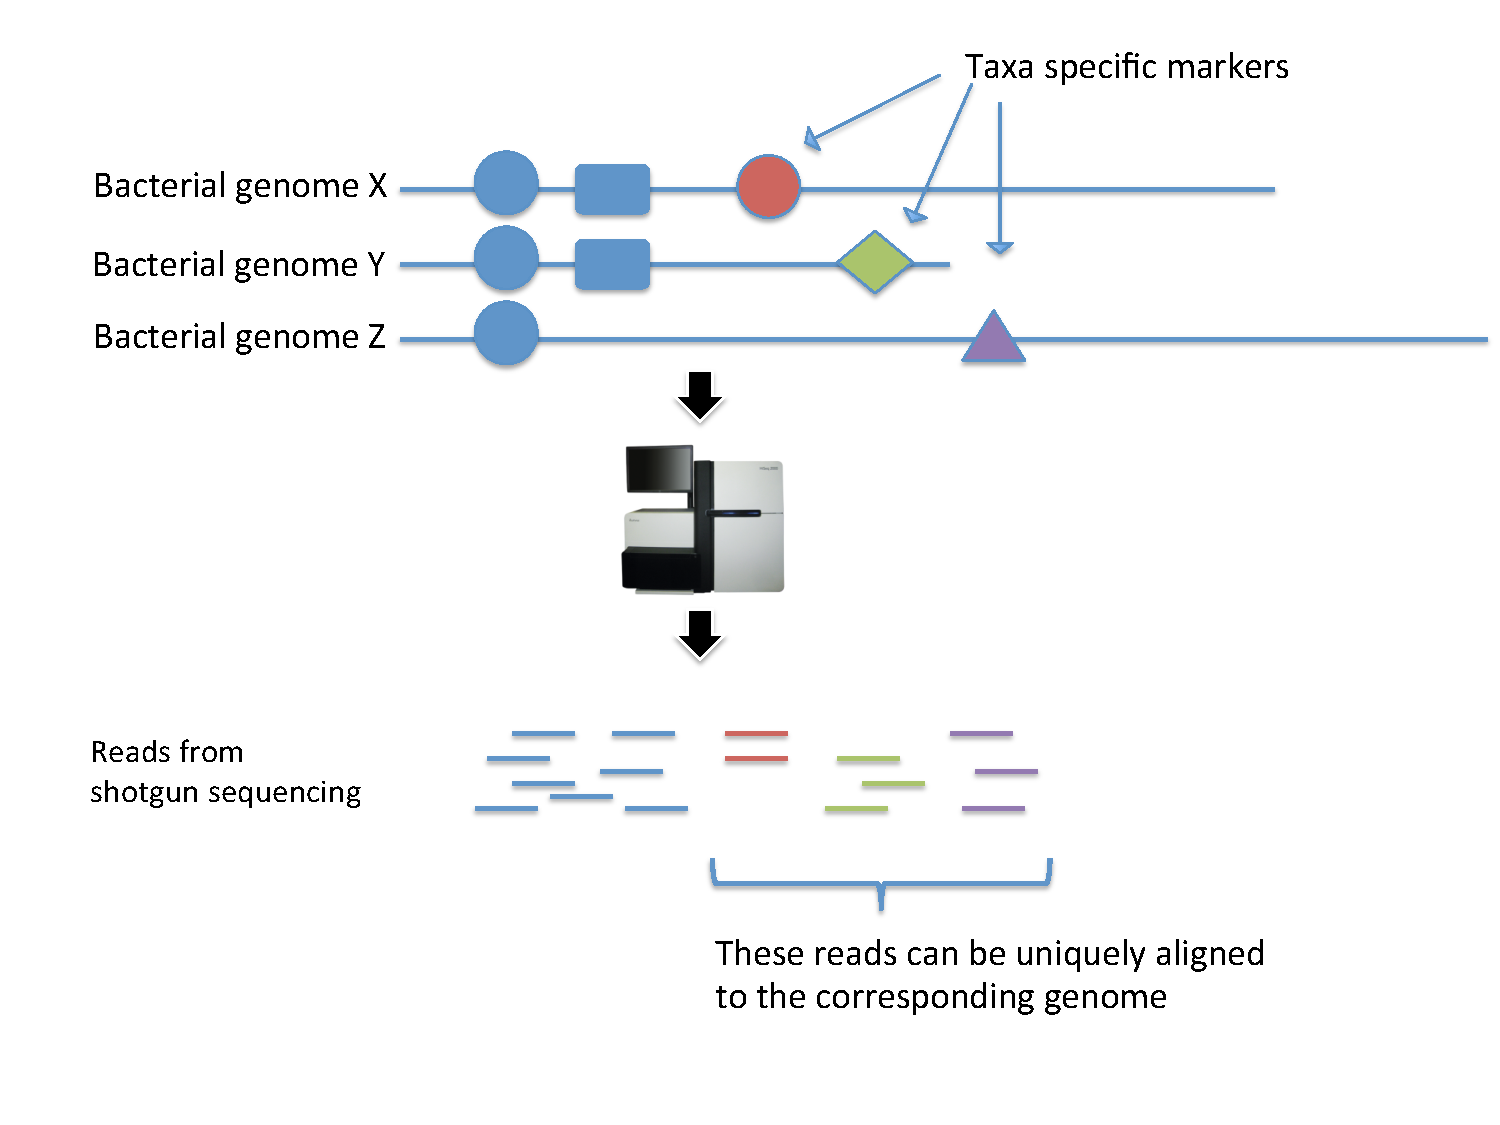
\includegraphics[scale=0.55,trim=0 0 0 0,clip]{Figure/F11_MetaPhlAn.pdf}
		\caption[An illustration of marker-based analysis strategy  for shotgun metagenomic data]{An illustration of marker-based analysis strategy  for shotgun metagenomic data. Taxa specific markers are identified by comparing known microbial genomes from public databases. Those taxa specific markers are then used as the references for alignment. Reads that fail to be aligned to the markers are discarded. Reads that can be aligned are used for quantifying microbial abundance.} \label{F11_MetaPhlAn}
	\end{center}
\end{figure}


Alternatively, shotgun sequencing of metagenomes, which sequences all genome sequences presented in the sample instead of just one marker gene, provides a more comprehensive approach to study human microbiome. This approach provides richer information about the microbial composition and gene functions. However, the analysis for shotgun sequencing data is more challenging than 16S rRNA sequencing data. One  difficulty is how to quantify the microbial abundance. Since the sequencing reads are generated from the whole genomes and microbial genomes share great similarity, it is difficult to uniquely align the reads back to the corresponding reference genomes. This makes the task of abundance quantification quite challenging. Currently, the most widely used strategy is to utilize  marker genes, either universal  markers \citep{Sunagawa:2013if} or taxa specific markers \citep{segata2012metagenomic}. For example, MetaPhlAn compares currently known microbial genomes from public databases and identifies taxa specific markers \citep{segata2012metagenomic}. Those taxa specific markers are then used as the references for alignment. Reads that fail to be aligned to the markers are discarded. Reads that can be aligned are used for quantifying microbial abundance. The marker-based analysis strategy used by MetaPhlAn is demonstrated in Figure~\ref{F11_MetaPhlAn}. 


This dissertation focuses  on statistical and computational methods for analysis of shotgun metagenomic data, motivated by Penn microbiome study of pediatric Crohn's disease. 


\section{Penn microbiome study of pediatric Crohn's disease}
Inflammatory bowel disease (IBD) is a disease involving chronic inflammation of gastrointestinal track. IBD can be categorized by the location of the inflammation into two forms, Crohn's disease (CD) and ulcerative colitis (UC). The symptoms of IBD include severe diarrhea, pain, fatigue and weight loss. The cause of the IBD is not entirely known although it is known to associate with abnormal host immune response. Recent studies show that the gut microbiome may play a role in the IBD onset \citep{gevers2014treatment} but the mechanism is not completely understood. Although treatments for IBD are available, currently there is no effective treatment to cure IBD without remission or relapse. One commonly used treatment is anti tumor necrosis factor (anti-TNF) treatment, which uses antibodies directed against host immune protein tumor necrosis factor $\alpha$ (TNF$\alpha$) to suppress immune response of the host. Anti-TNF treatment is not expected to alter the gut microbiome composition directly and is  reported to have side effects including increased risk of infection \citep{Borrelli:2006tk, Rutgeerts:2012ul}. Another treatment is enteral nutrition treatment, also called diet treatment, which feeds patients with defined formula diet. It possibly alters the gut microbiome composition. Diet treatment avoids immunosuppression but is difficult to maintain a long term effect \citep{Grover:2013dj}. The mechanisms of these treatments are not entirely clear.

\begin{figure}[p]
	\begin{center}
		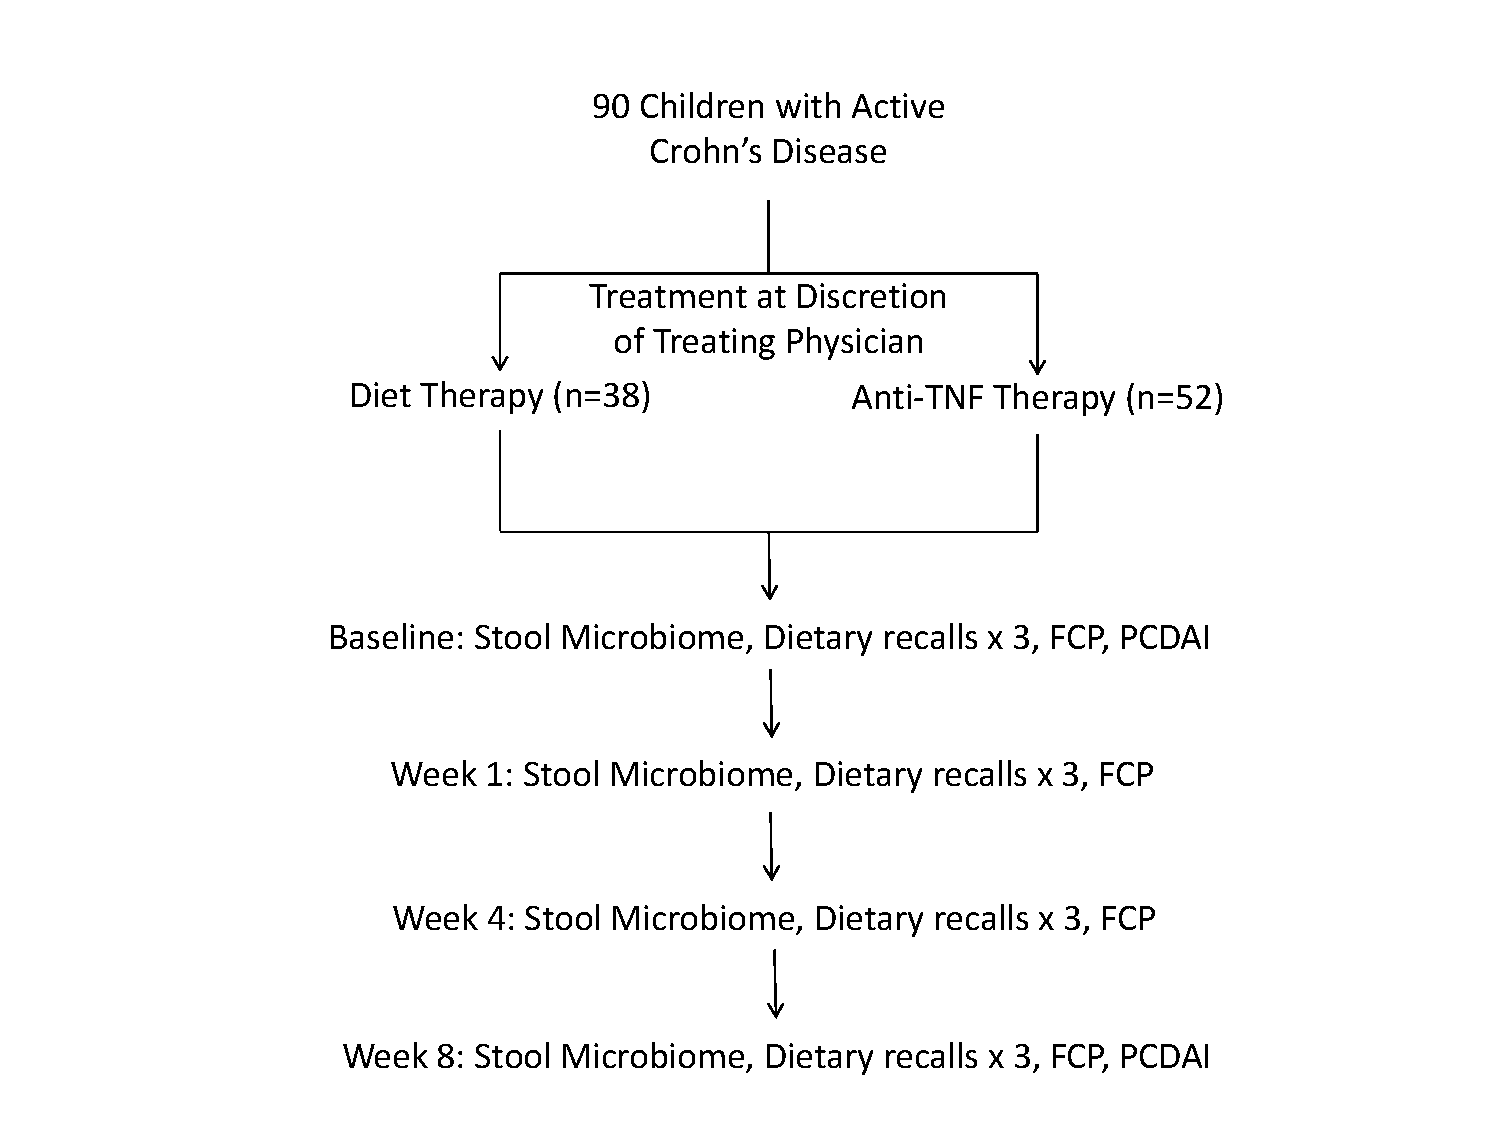
\includegraphics[scale=0.60,trim=40 0 0 0,clip]{Figure/F12_PLEASE_Study.pdf}
		\caption[An illustration of the PLEASE study at University of Pennsylvania.]{An illustration of the Penn Pediatric Longitudinal Study of Enteral Nutrition Therapy and Stool Microbiome Composition (PLEASE) study. This is a collaborative work with Dr. Gary Wu (Department of Gastroenterology), Dr. Rick Bushman (Department of Microbiology), Dr. Jim Lewis (Department of Epidemiology) and people in their research groups. } \label{F12_PLEASE_Study}
	\end{center}
\end{figure}




To improve our understanding of the role of human gut microbiome in Crohn's disease pathogenesis and how microbiome is associated with treatment response, we carried out a microbiome study, Pediatric Longitudinal Study of Enteral Nutrition Therapy and Stool Microbiome Composition (PLEASE)  at University of Pennsylvania (Penn) and The Children's Hospital of Philadelphia (CHOP). This is a collaborative work with Dr. Gary Wu (Department of Gastroenterology), Dr. Rick Bushman (Department of Microbiology), Dr. Jim Lewis (Department of Epidemiology) and people on their teams. The basic study design is illustrated  in Figure~\ref{F12_PLEASE_Study}.  In this study, we recruited a prospective cohort of pediatric Crohn's disease patients (ninety children) and collected their fecal samples as well as clinical data. The patients started therapy with either enteral nutrition or anti-TNF$\alpha$ antibodies (52 anti-TNF; 22 exclusive enteral nutrition [EEN]; 16 partial enteral nutrition with ad lib diet [PEN]). Stool samples were collected at four time points: baseline, 1 week, 4 weeks, and 8 weeks into therapy. We analyzed fecal samples using shotgun metagenomic sequencing approach.


\section{Dissertation organization }

This dissertation is structured as following. Chapter 2 presents the Penn microbiome study of pediatric Crohn's disease. In this project, we collected stool samples and clinical data from a prospective cohort of pediatric Crohn's disease patients, who started therapy with enteral nutrition or anti-TNF$\alpha$ antibodies. The fecal samples were analyzed by shotgun metagenomic sequencing approach. The results reveal the full complement and dynamics of bacteria and fungi during treatment. Bacterial community membership was associated independently with dysbiosis, intestinal inflammation, antibiotic use, and therapy.

Motivated by the problems in real data analysis, this dissertation also presents two statistical models for microbiome data analysis. Chapter 3 presents a multi-sample Poisson model to quantify microbial abundances. One important aspect of metagenomic data analysis is to quantify the bacterial abundances based on the sequencing data. In order to account for certain systematic differences in read coverage along the genomes, we propose a multi-sample Poisson model to quantify microbial abundances based on read counts that are assigned to species-specific taxonomic markers. Our model takes into account the marker-specific effects when normalizing the sequencing count data in order to obtain more accurate quantification of the species abundances.  The estimated maker-specific effects have further biological interpretations. 

Chapter 4 presents  statistical models  for longitudinal microbiome data analysis. A key question in longitudinal microbiome studies is to identify the microbes that are associated with clinical outcomes or environmental factors. A zero-inflated Beta regression model with random-effects (ZIBR) is developed for testing the association between microbial abundance and clinical covariates for longitudinal microbiome data. The model includes a logistic regression component to model presence/absence of a microbe in samples and a Beta regression component to model non-zero microbial abundance, where each component includes a random effect to take into account the correlations among the repeated measurements on the same subject. The statistical methods were evaluated using simulations as well as the real data analysis from Penn microbiome study of pediatric Crohn's disease.

All the analyses included in this dissertation were carried out in a  reproducible research fashion. Chapter 5 briefly demonstrates the examples of reproducible research for the three projects presented in the dissertation.

Finally, Chapter 6  presents conclusions and outline the future research directions. The three projects presented in Chapters 2, 3 and 4 are self-contained. Readers who are interested in individual project can read the corresponding chapter without referring to other ones.



%% --------------- PLEASE -------------------%%
\chpt{Inflammation, Antibiotics, and Diet as Environmental Stressors of the Gut Microbiome in Pediatric Crohn's Disease} \label{chpt2:please}

In the chapter, we present the Penn microbiome study of pediatric Crohn's disease. Dysbiosis, which is signified by abnormal composition of intestinal bacteria, is characteristic of Crohn's disease. Disease treatments include dietary changes and immunosuppressive anti-TNF$\alpha$ antibodies as well as ancillary antibiotic therapy, but their effects on microbiota composition are undetermined. Using shotgun metagenomic sequencing, we analyzed fecal samples from a prospective cohort of pediatric Crohn's disease patients starting therapy with enteral nutrition or anti-TNF$\alpha$ antibodies and reveal the full complement and dynamics of bacteria and fungi during treatment. Bacterial community membership was associated independently with intestinal inflammation, antibiotic use, and therapy. Antibiotic exposure was associated with increased dysbiosis, whereas dysbiosis decreased with reduced intestinal inflammation. Fungal proportions increased with disease and antibiotic use. Dietary therapy had independent and rapid effects on microbiota composition distinct from other stressor-induced changes and effectively reduced inflammation. These findings reveal that dysbiosis results from independent effects of inflammation, diet, and antibiotics and shed light on Crohn disease treatments. The work in this chapter has been published and readers who are interested in this work can refer to \citet{lewis2015inflammation, lee2015comparative}.


This project is a collaborative work with Gary Wu (Department of Gastroenterology), Rick Bushman (Department of Microbiology), Jim Lewis (Department of Epidemiology) and people in their teams. They recruited the subjects, collected samples and clinical data, prepared and sequenced the samples. My role in this project is to analyze the data and generate the report.

\section{Introduction}
The human gut microbiota is densely populated by microbes from all three domains of life together with their viruses \citep{Hoffmann:2013gu,Consortium:2012tm,Minot:2011ez}. Crohn's disease results from a pathologic interaction between the mucosal immune system and the environment, particularly the microbes residing in the gut lumen \citep{Sartor, Sartor:2008cs}, and is characterized by dysbiotic gut bacterial composition \citep{Huttenhower:2014ba, Khor:2011ky, Sartor, Sartor:2008cs}. Numerous human genetic loci encoding proteins involved in host immune responses have been linked to Crohn's disease \citep{Jostins:2012iu}, but the impact of these genes on the dysbiosis associated with Crohn's disease is limited \citep{Knights:2014jta}. Rather, dysbiosis is hypothesized to be a response of the microbes, particularly bacteria, to environmental stressors such as the host inflammatory response \citep{Huttenhower:2014ba} and/or the production of electron acceptors that facilitate anaerobic respiration \citep{Winter:2014ed}. Dysbiosis is commonly characterized by an expansion of Proteobacteria and a decrease in Firmicutes, along with a decrease in community richness \citep{nagalingam2012role}. Much less is known about the responses of other domains of microbial life to environmental stressors. Similarly, it is unknown whether dysbiosis resulting from inflammation is rapidly reversible. Patients with Crohn's disease are exposed to antibiotics and dietary changes that are likely to affect the microbiota, but the influence of these factors and their interactions with each other are incompletely understood. 

Antibiotics are often used as an ancillary therapy for Crohn's disease \citep{Khan:2011vo}. However, the main therapies for Crohn's disease includes episodic or chronic immunosuppression with corticosteroids, antimetabolite agents, or antibodies directed against host immune proteins such as tumor necrosis factor a (anti-TNF) \citep{Borrelli:2006tk, Grover:2013dj, Rutgeerts:2012ul}. The anti-TNF medications are administered parenterally and are not expected to alter the gut microbiota composition directly. An alternative therapy, used predominantly in children, is the defined formula diet, also known as enteral nutrition therapy. Both elemental and polymeric formulae, containing, respectively, amino acids and intact protein, have proved efficacious in treating symptoms and intestinal inflammation in Crohn's disease in addition to supporting nutritional needs for growth and weight maintenance \citep{Borrelli:2006tk,Grover:2013dj}. The efficacy of these diets is greatest when used as the exclusive source of nutrition \citep{Grover:2013dj,lee2015comparative}. Dietary therapy has the advantage of avoiding immunosuppression but is difficult to maintain long term. If the mechanism of action of dietary-based therapies were understood, it might be possible to develop less restrictive diets that deliver the same therapeutic benefit. One hypothesis is that diet therapy alters the composition of the gut microbiota in a manner that contributes to the therapeutic benefit, though data supporting this are limited \citep{Gerasimidis:2014gi,Kaakoush:2015hh}.


We reasoned that longitudinal characterization of the gut microbiome of pediatric Crohn's disease patients initiating therapy would allow us to characterize the concurrent effects of intestinal inflammation, antibiotics, and diet on gut microbial community structure. We conducted a longitudinal study of 90 children with Crohn's disease who were initiating treatment with either a defined formula diet or anti-TNF therapy and compared them to 26 healthy control children. We tracked symptoms, mucosal inflammation, and changes in the gut microbiome over an 8-week study period. The gut microbiome was quantified using shotgun metagenomic DNA sequence analysis of longitudinal samples. Dysbiosis was quantified as the distance of each sample from the centroid of samples from healthy controls. Communities partitioned into two distinct clusters based on the bacterial composition, as seen previously \citep{Frank:2007hn, gevers2014treatment}, one of which overlapped the healthy controls. The dysbiotic community was associated with increases in specific fungi, prior antibiotic therapy, and higher concentration of human DNA in feces. By tracking the microbiota composition over the course of therapy, we found that dysbiosis was reduced in response to decreased bowel inflammation, and that inflammation, antibiotic exposure, and diet independently influenced different taxa. Fungi were elevated with disease and antibiotic use, but diminished with diet therapy. Thus while dysbiosis in the gut is common in Crohn's disease, the response of the gut microbiome depends on the environmental stressor.


\section{Clinical outcomes in patients treated with a defined formula diet versus anti-TNF}
Ninety children initiated one of the study therapies (52 anti-TNF; 22 exclusive enteral nutrition [EEN]; 16 partial enteral nutrition with ad lib diet [PEN]) \citep{lee2015comparative}. EEN- and PEN-treated children consumed approximately 90\% and 53\% of daily calories from dietary formulas, respectively. Inflammation was quantified by measuring fecal calprotectin (FCP). Response to therapy was defined as a reduction of FCP to below 250 mg/g because this measure is associated with diminished mucosal inflammation \citep{Lin:2014hm}. Reduction in FCP below 250 mg/g was more common among those receiving anti-TNF (62\%) and EEN (45\%) than PEN (10\%) \citep{lee2015comparative}.



\section{Microbial community patterns in Crohn's disease and healthy controls}
Adequate stool samples were available from 86 individuals to conduct shotgun metagenomic analysis. Samples were collected at four time points: baseline, 1 week, 4 weeks, and 8 weeks into therapy (Table~\ref{TS1}). We also compared stool samples from 26 healthy children collected in a prior study \citep{wu2011linking} but analyzed by shotgun metagenomic sequencing here. None of the healthy children had received antibiotics in the prior 6 months. DNA was prepared from whole stool, and sequenced using the Illumina HiSeq paired-end method. After filtering out low-quality, human, and contami- nating reads, we were left with $6.5 \times 10^{11}$ bases of microbial DNA sequence for analysis.



We quantified the bacterial taxonomic composition using MetaPhlAn \citep{segata2012metagenomic}. Figure~\ref{Fig21_Microbiome_Cluster_Heatmap} shows a comparison of bacterial lineages in the healthy control subjects and pediatric Crohn's disease cohort prior to initiation of therapy ("baseline" in the below). Figure~\ref{Fig21_Microbiome_Cluster_Heatmap}A shows taxonomic proportions for each sample at baseline with metadata summarized above the heat map (all time points are shown in Figure~\ref{F2S1_heatmap}). 


\begin{figure*}[p]
\centering
{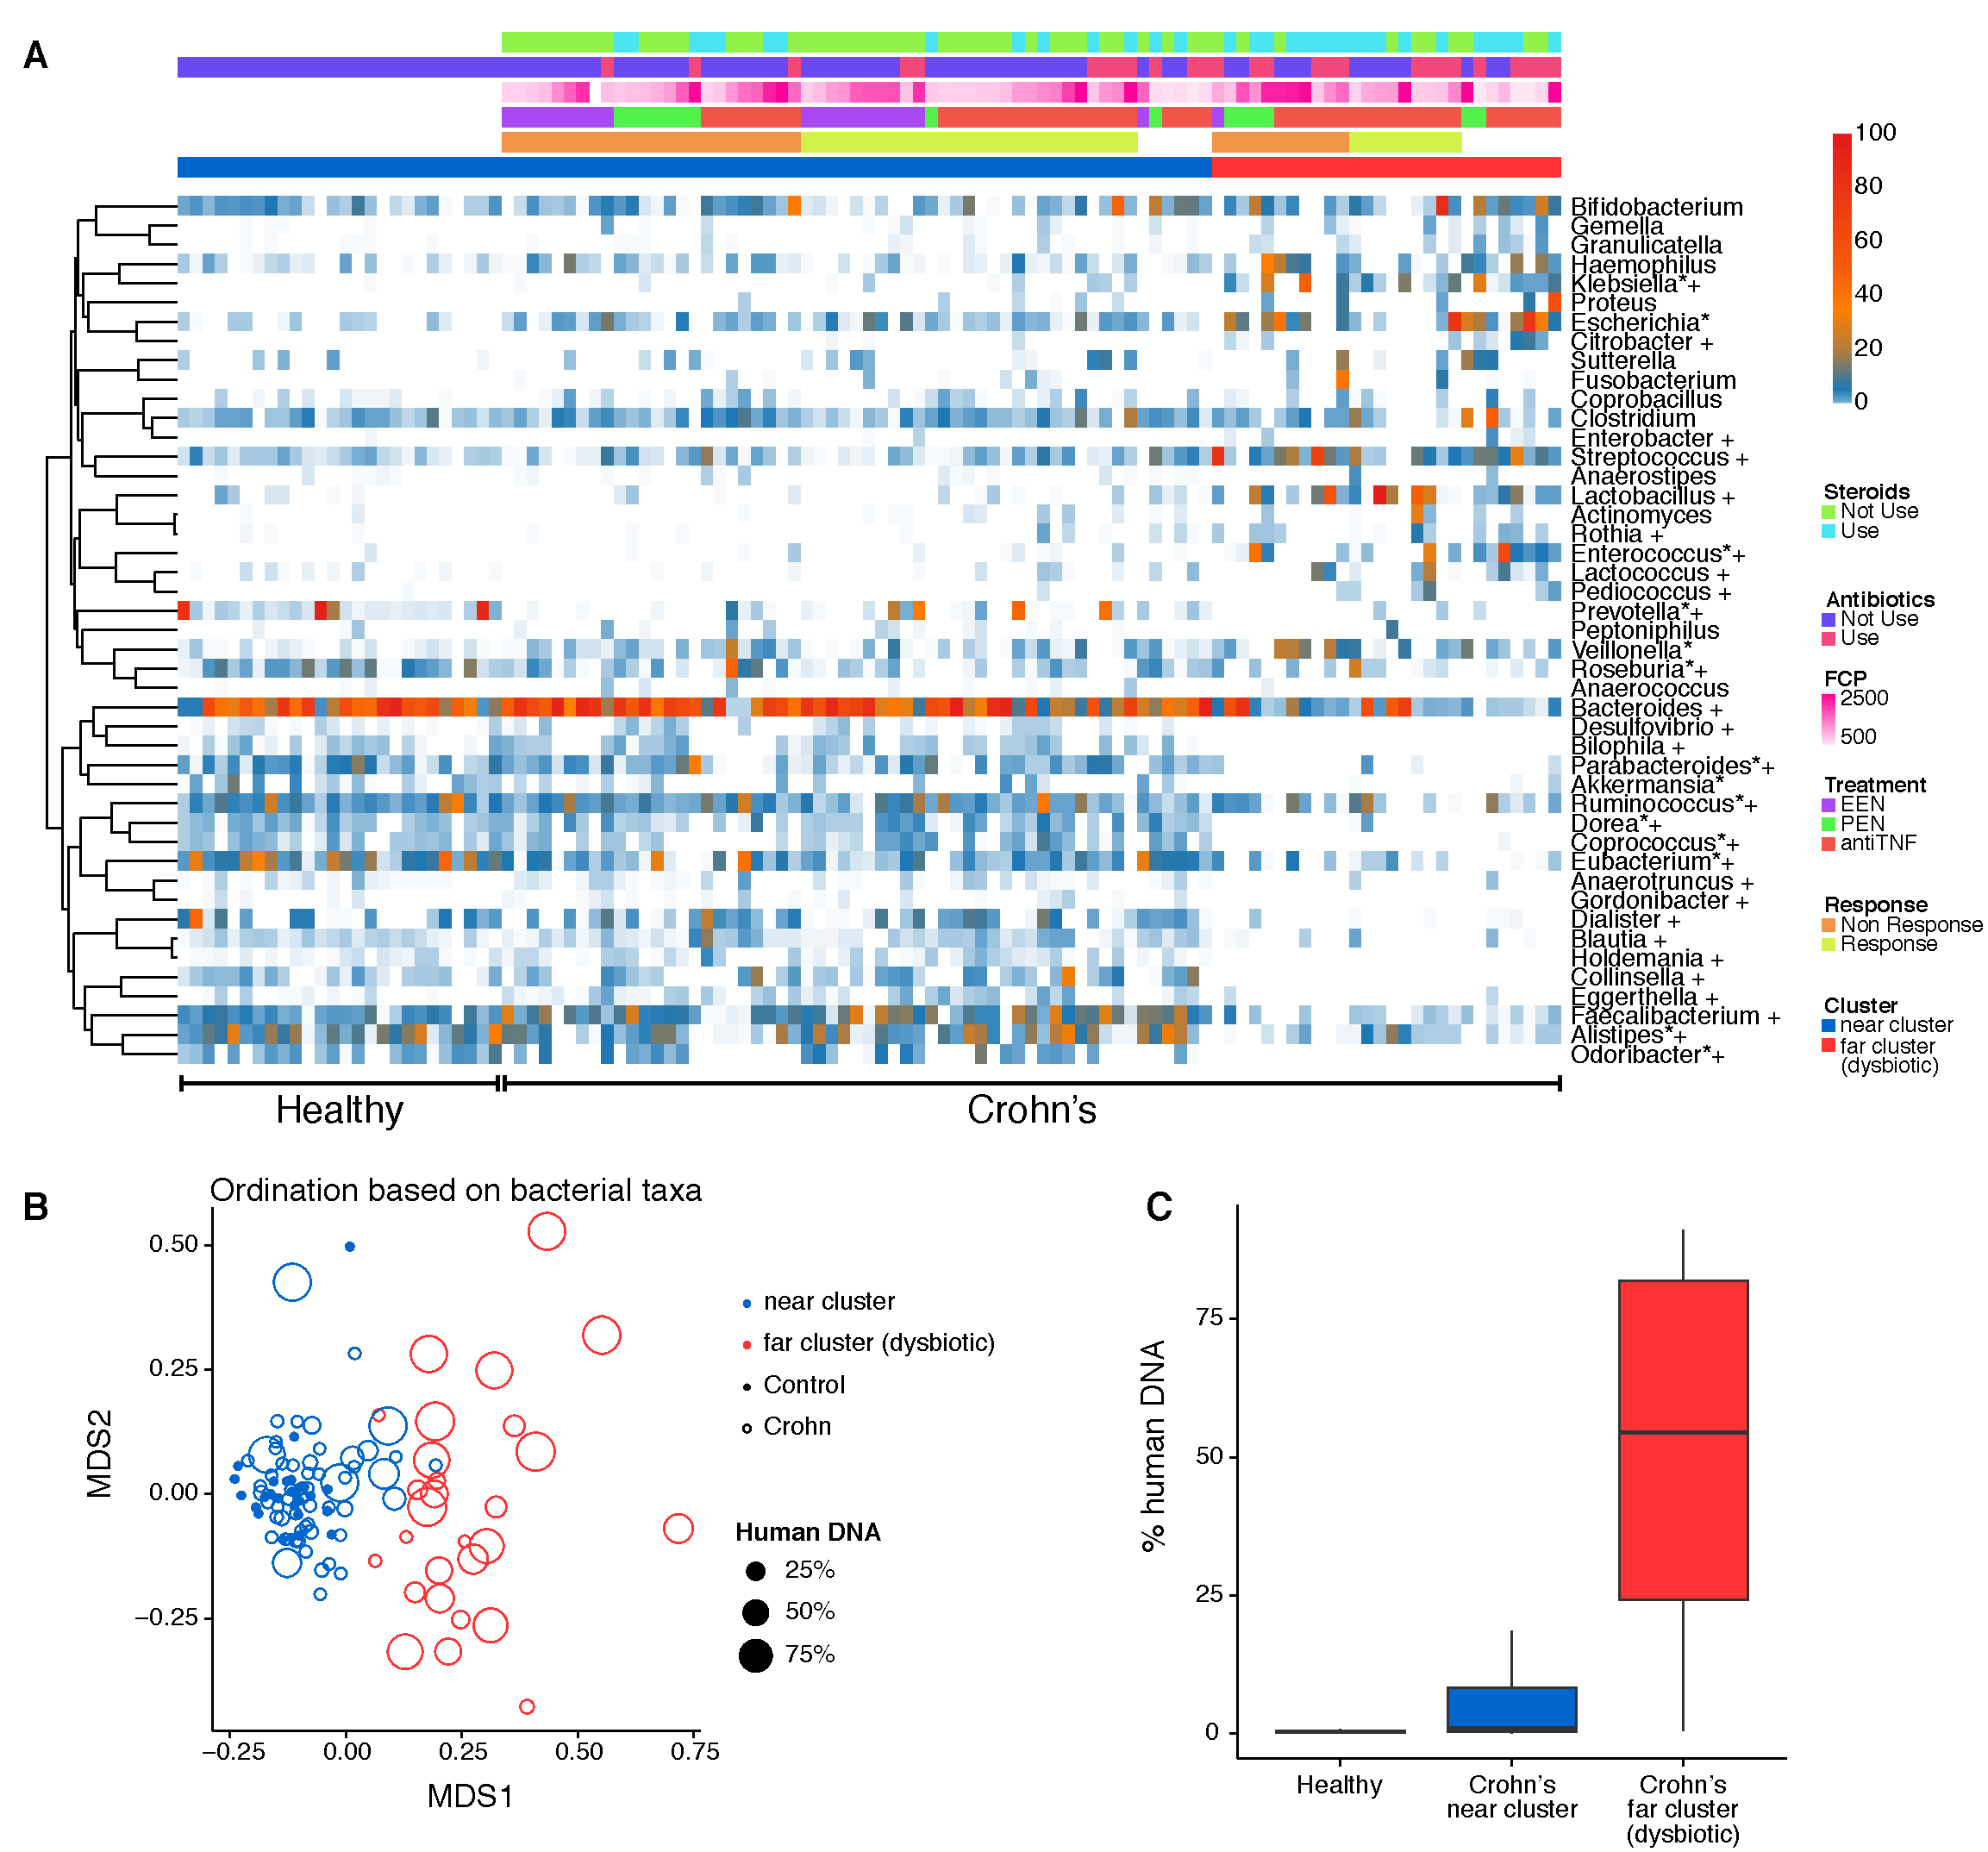
\includegraphics[scale=0.37,trim=0 0 0 0,clip]{Figure/Fig21_Microbiome_Cluster_Heatmap.pdf}}
\caption[Bacterial composition in samples from children with Crohn's disease and healthy controls]{Bacterial composition in samples from children with Crohn's disease and healthy controls. (A) A heatmap demonstrating relative abundance of bacterial taxa prior to therapy according to presence or absence of Crohn's disease, cluster assignment, use of corticosteroids and antibiotics, FCP concentration, and response to therapy. Metadata are indicated by the color code at the top of the figure. White cells indicate missing data. Taxa that were statistically different in abundance between Crohn's disease and healthy controls are identified by *; taxa that were statistically different in abundance between the two Crohn's disease clusters are identified by + (q $<$ 0.05). FCP in this and subsequent figures indicates FCP. Samples were ordered by the metadata (healthy versus Crohn's samples, and cluster 1 versus cluster 2, then other forms of metadata).
(B) MDS analysis of samples from children with Crohn's disease and healthy controls. Bacterial taxa present were quantified by MetaPhlAn, distances were calculated using binary Jaccard Index, and samples were plotted based on MDS. Samples from healthy controls are shown by the filled circles, and Crohn's disease as open circles. Clusters were defined by partitioning around medoids with estimation of number of clusters (PAMK), and are colored blue (healthy associated) and red (dysbiotic). The size of the dot is scaled by the proportion of human DNA in the sample.
(C) Percentage of human DNA reads in each metagenomic sequence sample. Near cluster (blue, associated with healthy controls) and far cluster (red, dysbiotic) refer to the groups shown in (B). }
\label{Fig21_Microbiome_Cluster_Heatmap}
\end{figure*}


\begin{figure*}[p]
\centering
{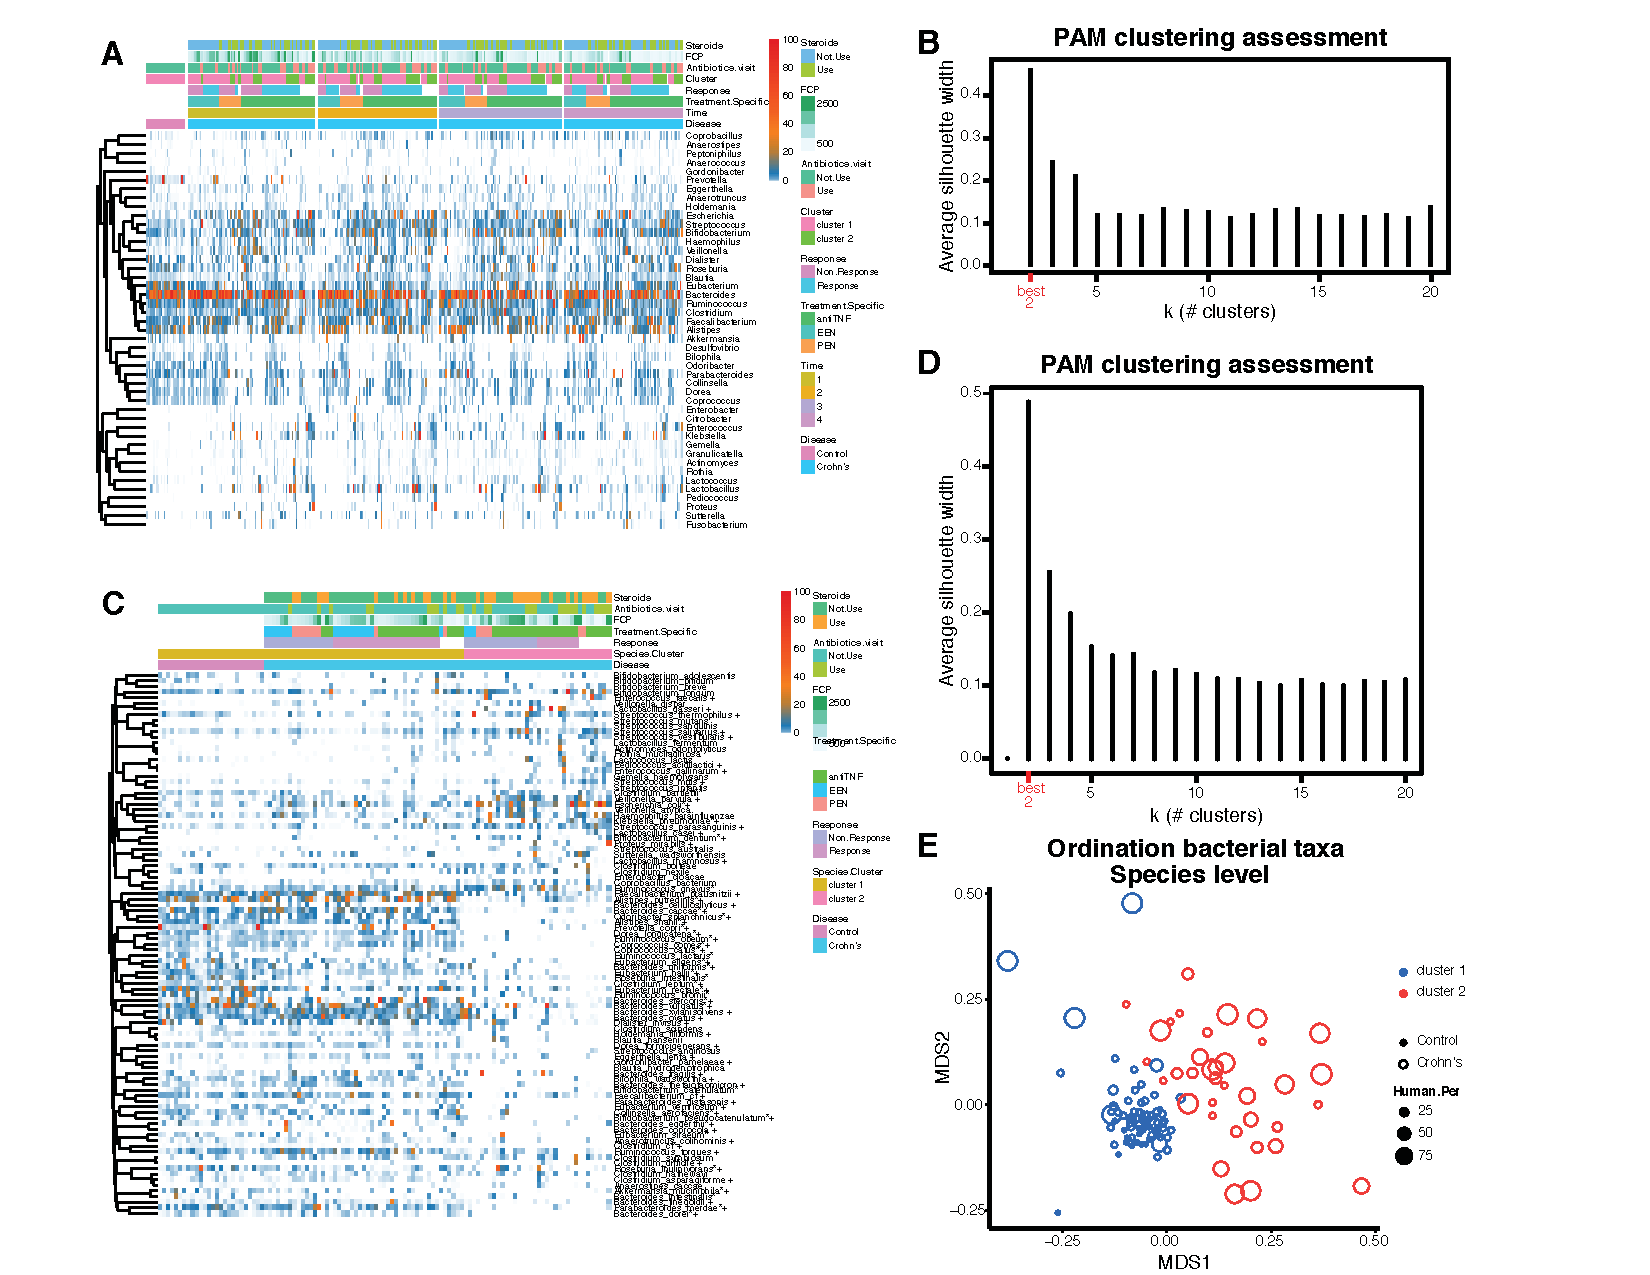
\includegraphics[scale=0.62,trim=20 0 0 0,clip]{Figure/F2S1_heatmap.pdf}}
\caption[Bacterial composition in samples across all time points and analysis on the species level]{Bacterial composition in samples across all time points and analysis on the species level. A) Heat map of genera detected over all time points and samples analyzed. Sample metadata is summarized at the top; a key to the metadata summarized is at the right. B) Silloutte score analysis of clustering by taxonomic composition at the genus level. The analysis specifies two as the optimal number of clusters. Separation is modest, so that data could also be described as a continuum. C) Analysis at the species level. Heat map of taxonomic proportions. Crohn’s disease and healthy controls are identified by *; taxa that were statistically different in abundance between the two Crohn’s disease clusters are identified by + (q$<$0.05). D) PAM analysis of clustering using species-level assignments. E) Ordination showing formation of two clusters using species-level data. }
\label{F2S1_heatmap}
\end{figure*}

\begin{figure*}[p]
\centering
{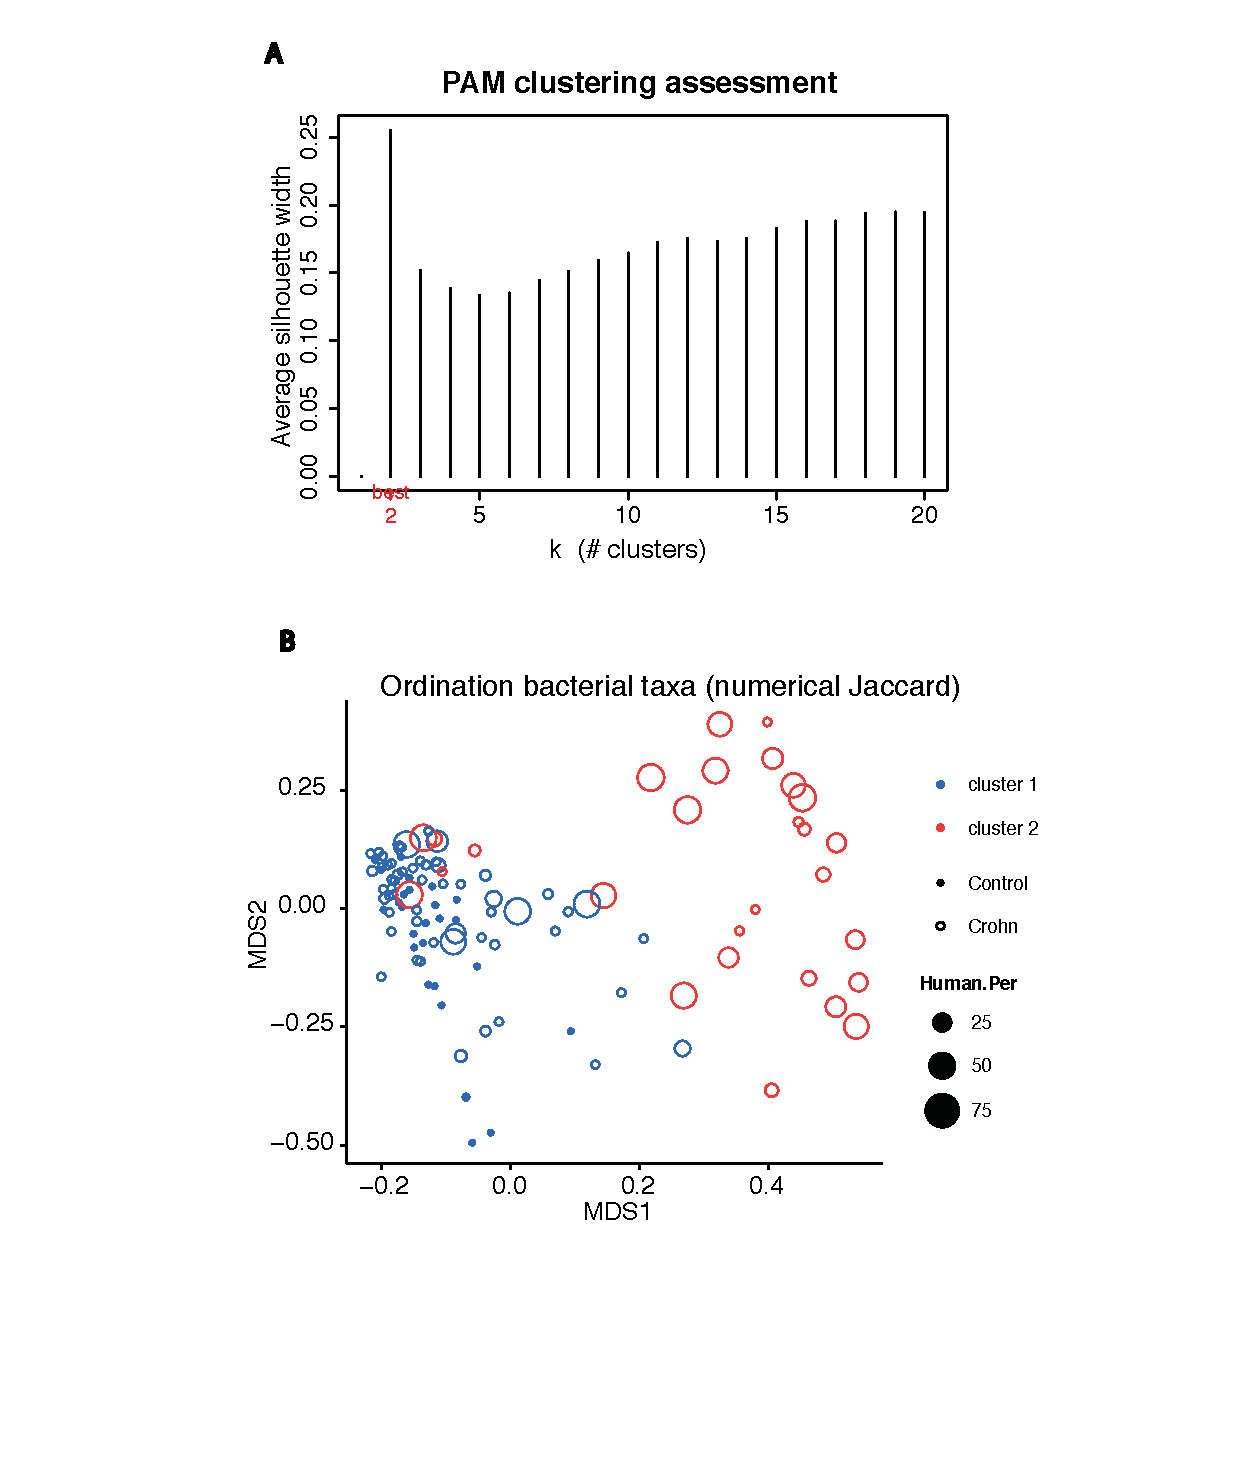
\includegraphics[scale=0.62,trim=50 100 0 0,clip]{Figure/F21_Numerical_Jaccard_MDS_Merge.pdf}}
\caption[PAM and MDS analysis using numerical Jaccard]{PAM and MDS analysis using numerical Jaccard. A)  PAM analysis of clustering  at the genus level with numerical Jaccard.  B) Ordination showing formation of two clusters using numerical Jaccard distance. }
\label{F21_Numerical_Jaccard_MDS_Merge}
\end{figure*}


After filtering out very-low-abundance genera, comparison of median relative abundances showed 14 of 45 genera differed between children with Crohn's disease and healthy controls (FDR controlled p $<$ 0.05 by Wilcoxon rank-sum test; Table~\ref{TS2}). The Crohn's patients had reduced relative abundance of Prevotella, Eubacterium, Odoribacter, Akkermansia, Roseburia, Parabacteroides, Alistipes, Coprococcus, Dorea, and Ruminococcus and increased abundance of Escherichia, Klebsiella, Enterococcus and Veillonella. Random forest was used to identify bacterial lineages that best distinguished healthy children from Crohn's patients with active disease, and predicted Crohn's disease and normal with 86\% prediction accuracy. Mostly similar lineages (Prevotella, Odoribacter, Eubacterium, Escherichia, and Faecalibacterium) were found to distinguish the groups.


Community patterns were analyzed using partitioning around medoids with estimation of number of clusters (PAMK) to find the optimal number of clusters, and visualized after multidimensional scaling (MDS) (Figure~\ref{Fig21_Microbiome_Cluster_Heatmap}B). Samples from patients with active Crohn's disease partitioned into two clusters (Figure~\ref{F2S1_heatmap}B): one that was near to the healthy controls (near cluster) and one that clustered separately (far dysbiotic cluster), paralleling previous studies \citep{Frank:2007hn, gevers2014treatment}. Thirty of 45 genera differed in abundance (q $<$ 0.05) between the two clusters (Table~\ref{TS3}). The far dysbiotic cluster was characterized by an increased relative abundance of Streptococcus, Klebsiella, Lactobacillus and reduced relative abundance of Faecalibacterium, Parabacteroides, Dorea, Blautia, Holdemania, Collinsella, Coprococcus, Odoribater, Prevotella, Bacteroides, Dialister, Eubacterium, Alistipes, and Ruminococcus. Random forest with bacterial abundance had 92\% prediction accuracy for predicting these two clusters. The top five most predictive genera were Blautia, Faecalibacterium, Dialister, Lactobacillus, and Bacteroides. 

To make sure the two-cluster pattern and its correlation with human DNA in the previous analysis is not due to artifacts, we repeated the clustering analysis and  MDS analysis at species level as well as using another distance index, numerical Jaccard distance. The analysis at the species level (Figures~\ref{F2S1_heatmap}C and \ref{F2S1_heatmap}D) and analysis using numerical Jaccard distance (Figures~\ref{F21_Numerical_Jaccard_MDS_Merge}A and \ref{F21_Numerical_Jaccard_MDS_Merge}B) yielded similar conclusions. 


In summary, baseline samples clustered into two groups, with the far dysbiotic cluster being more distant from the healthy controls and characterized by altered bacterial composition and lower diversity.





\section{High levels of human DNA in stool correlated with dysbiosis}
In processing the metagenomic DNA from stool, we observed that the proportion of human DNA varied widely (Figure~\ref{Fig21_Microbiome_Cluster_Heatmap}C). The percentage of human reads was low in the healthy controls (mean = 0.87\%, max = 10.1\%, minimum = 0.05\%) relative to patients with active Crohn's disease (mean = 16.6\%, maximum = 94.2\%, minimum = 0.01\%; $p < 5 \times 10^{-11}$), with over 50\% of the sequence reads mapped to human in 49 Crohn's disease samples. Selected DNA samples were tested for human DNA content using QPCR to detect human beta-tubulin-coding sequences, revealing that the amounts detected were positively correlated with the calls from metagenomic sequencing (r = 0.81 Pearson's correlation, $p = 9.3 \times 10^{-11}$). We hypothesized that the source of human DNA was either epithelial cells or blood shed into feces associated with disease activity.


\section{Analysis of fecal microbial gene pathways}
The gene content of the gut microbiota was compared to assess associations between gene function and dysbiosis (Figure~\ref{F22_Pathway_Cluster_Heatmap}A) using HUMAnN \citep{Abubucker:2012fd} Differences were found between IBD and healthy controls in 42 of 163 pathways examined (Table~\ref{TS4}). Crohn's samples clustered into two groups based on gene pathway data, one of which more closely resembled the healthy controls and one more dysbiotic (Figure~\ref{F22_Pathway_Cluster_Heatmap}B; Table~\ref{TS5}). The clusters separated based on pathway data tracked closely with the near and far clusters defined by bacterial taxonomic representation (Figure~\ref{F22_Pathway_Cluster_Heatmap}B, red and blue colors). 

To guide interpretation, we analyzed the Spearman correlation between bacterial abundance and gene pathway enrichment in these data (Figure~\ref{F2S2_gene_heatmap}A). Pathway data partitioned the bacteria into two notable groups, one including gammaproteobacteria together with Streptococcus and Enterococcus and a second group dominated by Bacteroides and multiple anaerobic Bacteroidetes and Firmicutes typical of healthy gut. Below we propose relationships between specific gene pathways and persistence in the presence of different environmental stressors. However, enrichment may also be due to passenger effects, where outgrowth of specific organisms resulted in enrichment in pathways that were not themselves major contributors to differential fitness. 

Random forest was used to identify those pathways that best discriminated between healthy children and the active Crohn's disease cohort at baseline (Figures~\ref{F22_Pathway_Cluster_Heatmap}C and \ref{F2S2_gene_heatmap}B). Samples membership in the two categories could be predicted with 87\% accuracy using gene pathway data, comparable to the partitioning achieved using bacterial taxonomic data. The top six most notable pathways, higher in the Crohn's samples, were sulfur relay systems, galactose metabolism, biosynthesis of siderophores, glycerolipid metabolism, glutamine/glutamate metabolism, and nitrogen metabolism (Table~\ref{TS4}). Similarly, 94 of 163 gene pathways were differentially abundant between the two clusters, 51 with greater representation in the more dysbiotic far cluster (Table~\ref{TS5}). Random forest using gene pathway abundance had 87\% prediction accuracy for classification of the two bacterial clusters (near and far dysbiotic) defined by taxonomic proportions. The five most predictive pathways were glycerophospholipid metabolism, aminobenzoate degradation, sulfur relay system, and glutathione metabolism, which were increased in the far dysbiotic cluster, and selenocompound metabolism, which was decreased in the far cluster. Thirty-three of 42 pathways that were significantly different between Crohn's disease and healthy controls were also significantly different between the two clusters of Crohn's disease, suggesting that they are related primarily to the composition of the dysbiotic microbiota rather than being intrinsic alterations associated with IBD per se. 


\begin{figure*}[p]
\centering
{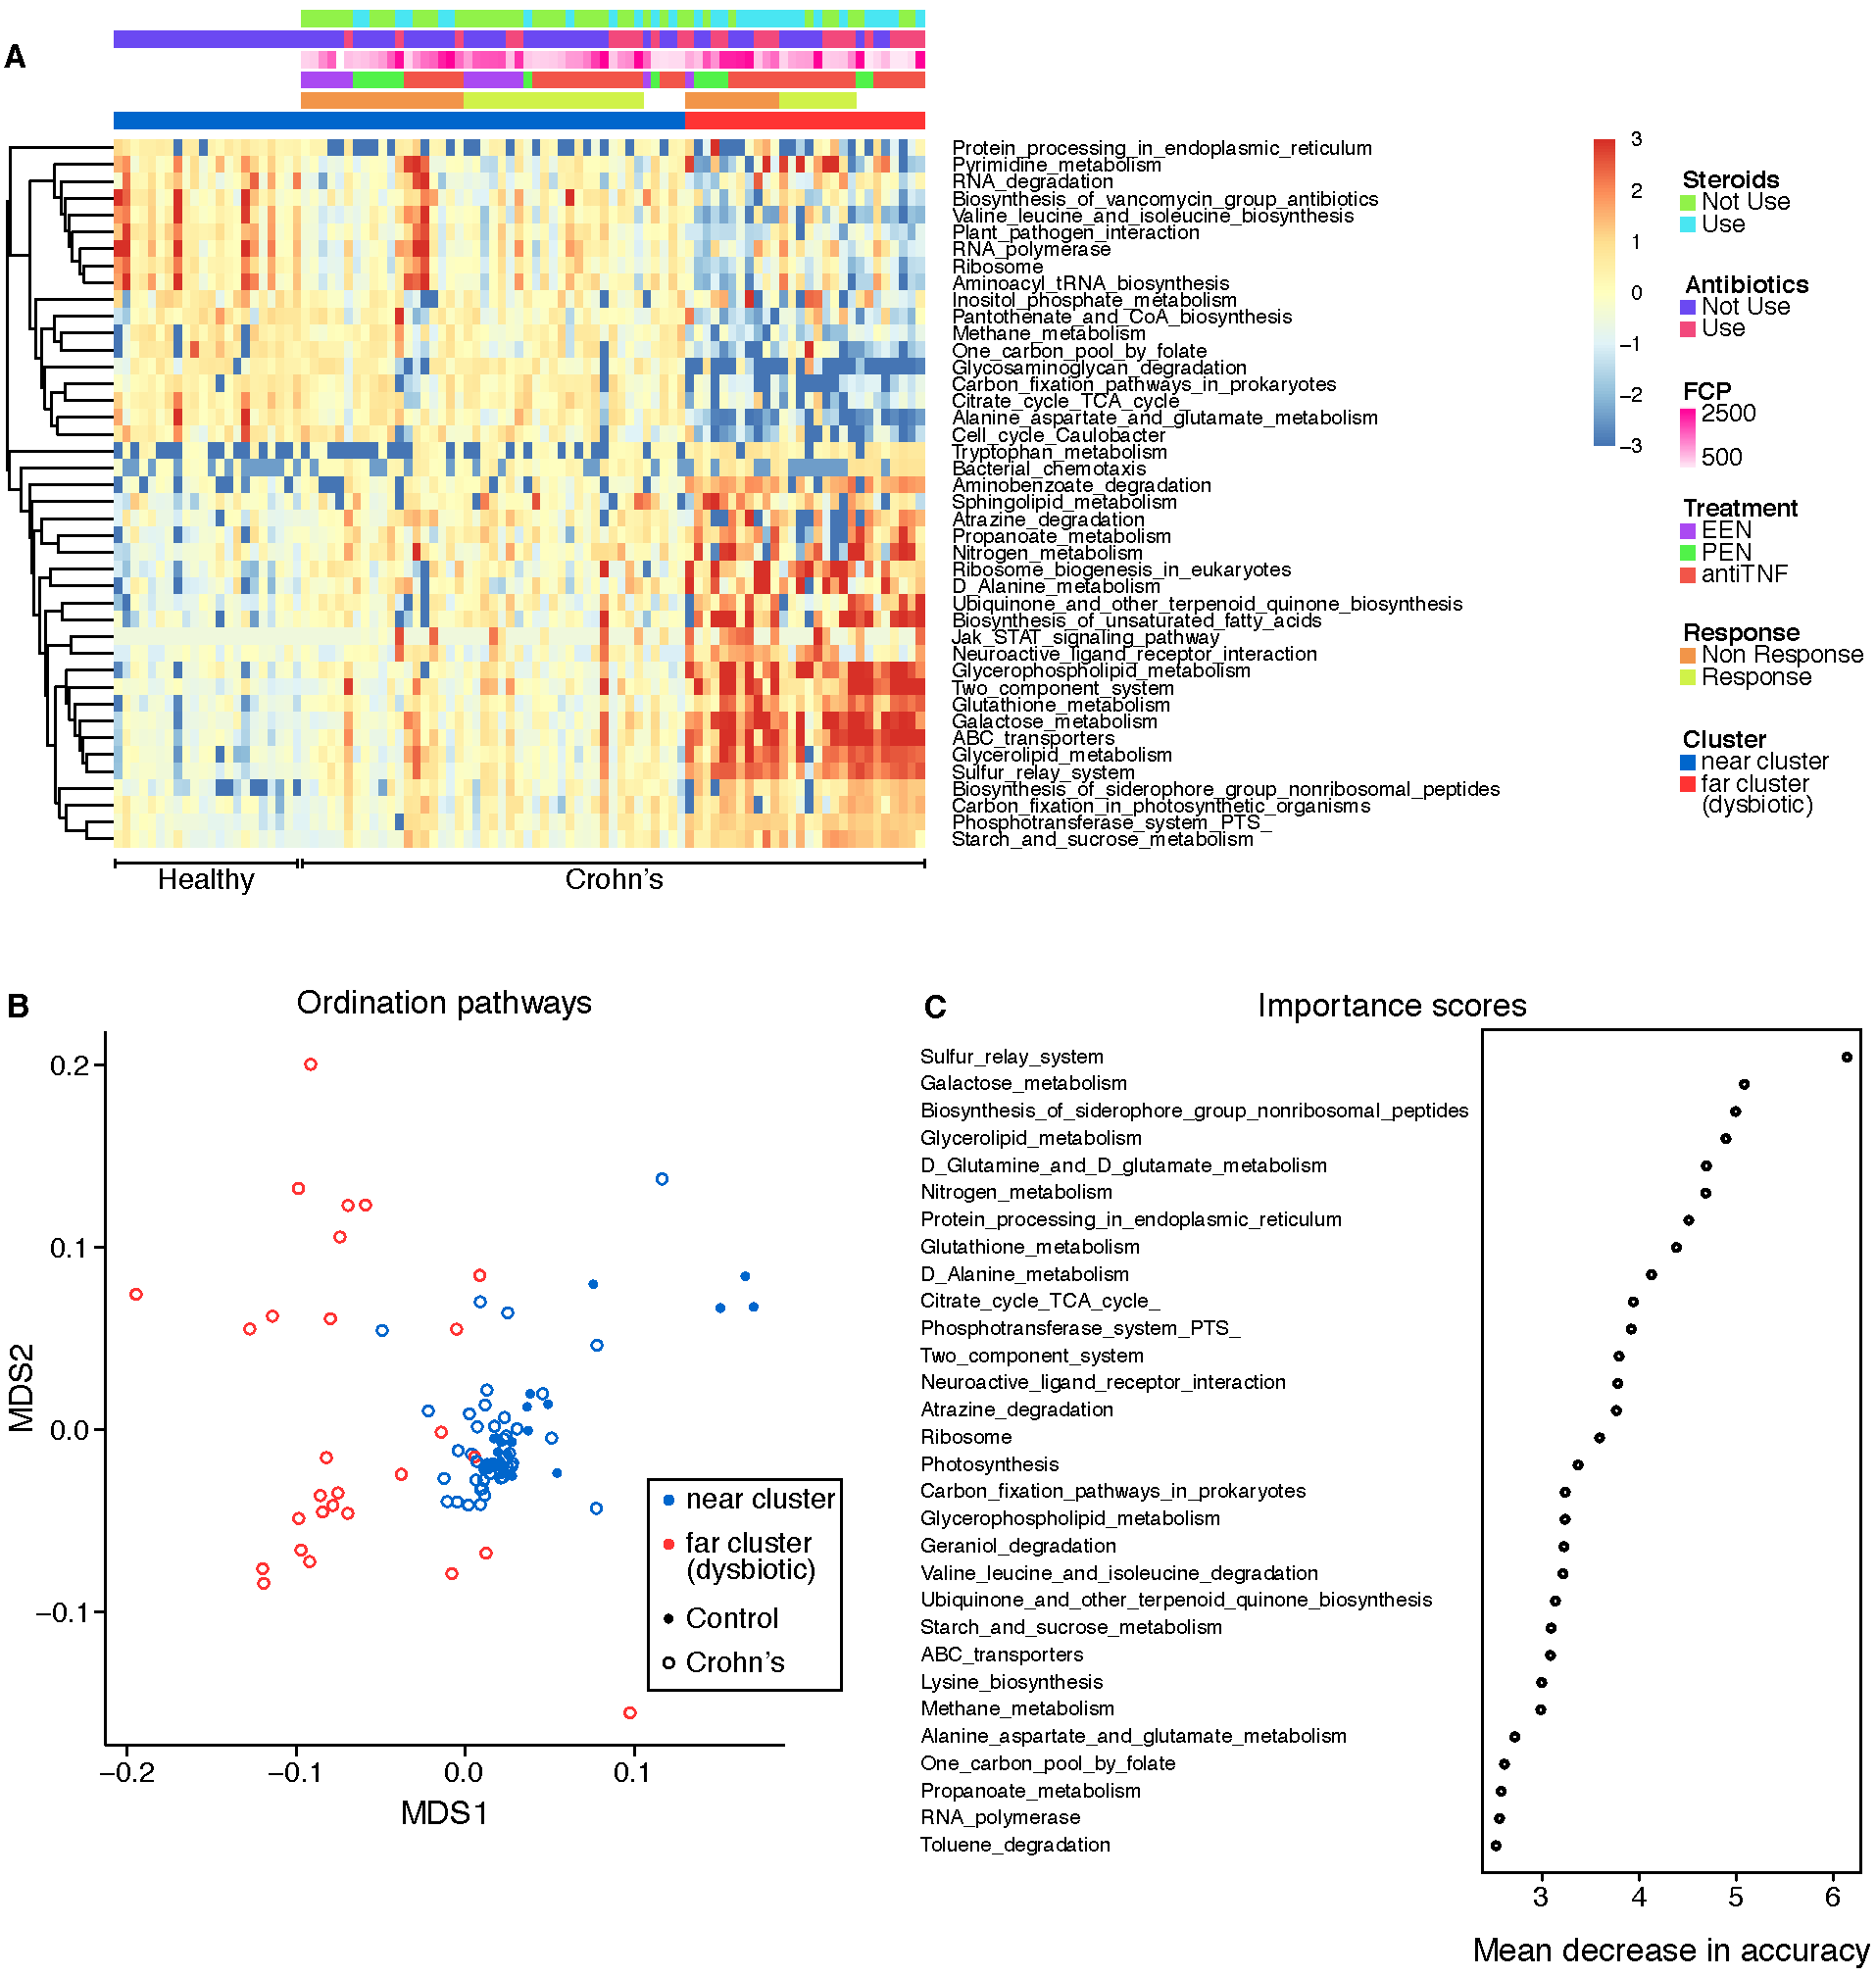
\includegraphics[scale=0.45,trim=0 0 0 0,clip]{Figure/F22_Pathway_Cluster_Heatmap.pdf}}
\caption[Comparison of gene pathways present in samples from Crohn's disease subjects and healthy controls at baseline]{Comparison of gene pathways present in samples from Crohn's disease subjects and healthy controls at baseline assessed by shotgun metagenomics.
(A) Heatmap of pathways that differed significantly (q value $<$ 0.05) between healthy controls and Crohn's disease subjects at baseline. Each row was normalized by z score.
(B) Cluster analysis based on MDS using the pathway data. Colors indicate samples that are members of the near cluster (overlapping healthy controls) or far cluster (dysbiotic) as defined by the analysis of bacterial taxa. Controls are defined by filled circles and Crohn's disease samples by open circles.
(C) Analysis using the machine learning algorithm Random Forest. Gene pathways that most strongly distinguish patients with Crohn's disease from healthy controls were identified. Importance scores were derived from the loss in accuracy measured when each indicated pathway was removed from the analysis. The units on the x axis indicate mean decrease in accuracy. }
\label{F22_Pathway_Cluster_Heatmap}
\end{figure*}




\begin{figure*}[p]
	\centering
	{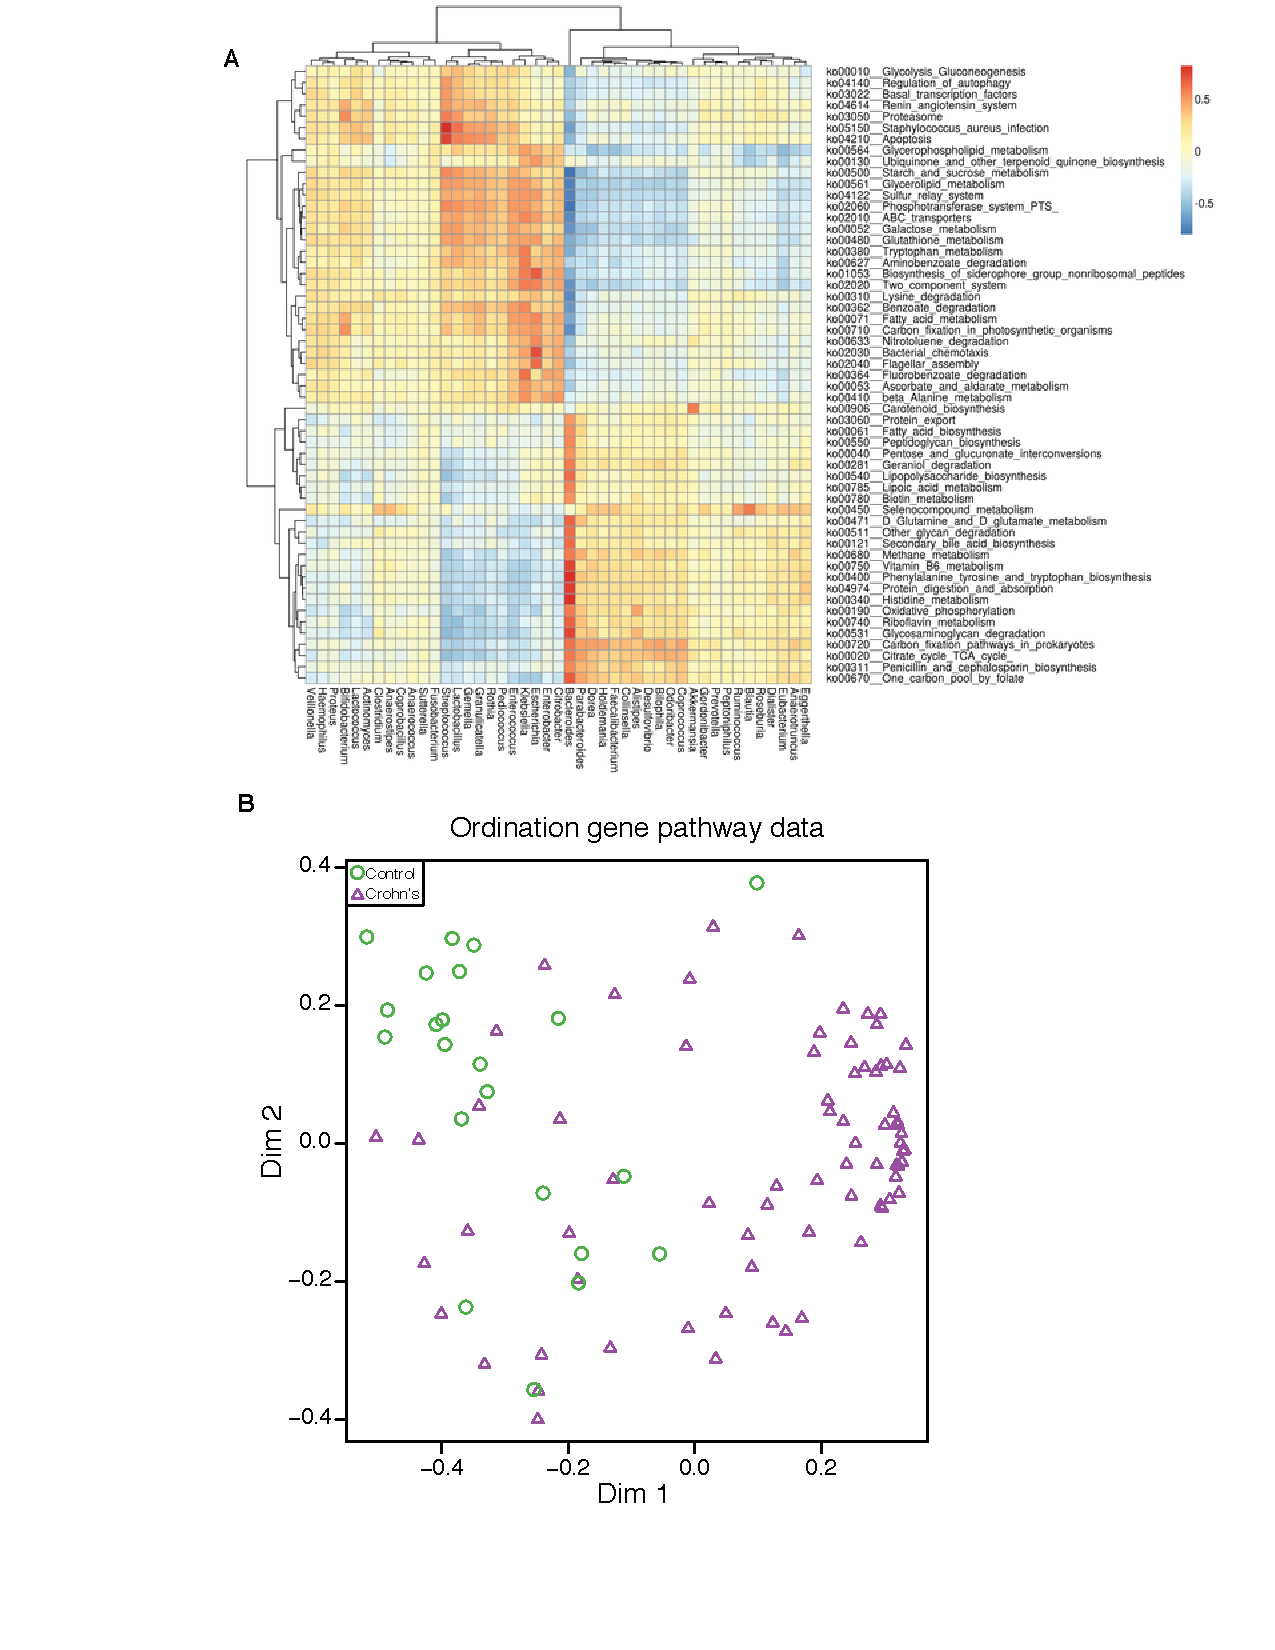
\includegraphics[scale=0.7,trim=0 40 0 0,clip]{Figure/F2S2_gene_heatmap.pdf}}
	\caption[Correlation of bacterial composition and KEGG pathways]{Correlation and ordination analysis of pathway data. A) Correlation of bacterial composition and KEGG pathways. The heat map plots the Spearman correlations among bacteria and pathways. B) Analysis of gene pathway representation in Crohn’s disease patients and healthy controls. MDS analysis of fecal samples clustered by pathway representation. 
	}
	\label{F2S2_gene_heatmap}
\end{figure*}




\section{Fungal community structure} 
We characterized the fungal reads in the metagenomic data by alignment to sequenced fungal genomes, followed by extensive filtering to remove artifacts. Five fungal taxa were detected in the samples—Saccharomyces cerevisiae, Clavispora lusitaniae (also known as Candida lusitaniae), Cyberlindnera jadinii (also known as Pichia jadinii and Candida utiliz), Candida albicans, and Kluyveromyces marxianus. Figure~\ref{F23_Fugus}A shows the representation of fungal taxa in healthy controls and Crohn's disease samples at baseline, and the relationship to metadata. All of the fungal taxa were more represented in the samples from Crohn's disease subjects, particularly those in the more dysbiotic far cluster as defined by the bacterial taxonomic analysis in Figure~\ref (Figures~\ref{F23_Fugus}B-\ref{F23_Fugus}F). Abundance of the different fungi were highly correlated with each other (Spearman correlation 0.66-0.84). Higher fungal proportions in samples also correlated with higher levels of human DNA (Figure~\ref{F23_Fugus}G). Random Forest analysis based on fungal data had 92\% prediction accuracy for classification of normal and baseline Crohn's disease samples. The most predictive fungus was Clavispora lusitaniae. Thus, the five yeasts detected are positively associated with Crohn's disease, particularly in the setting of greater bacterial dysbiosis. Some correlations were observed between bacteria and fungi in the cohort, but these varied between the healthy controls and the two clusters of patients with Crohn's disease (Figures~\ref{F2S3_taxa_fungi_correlation}A-\ref{F2S3_taxa_fungi_correlation}C).


\begin{sidewaysfigure}
\centering
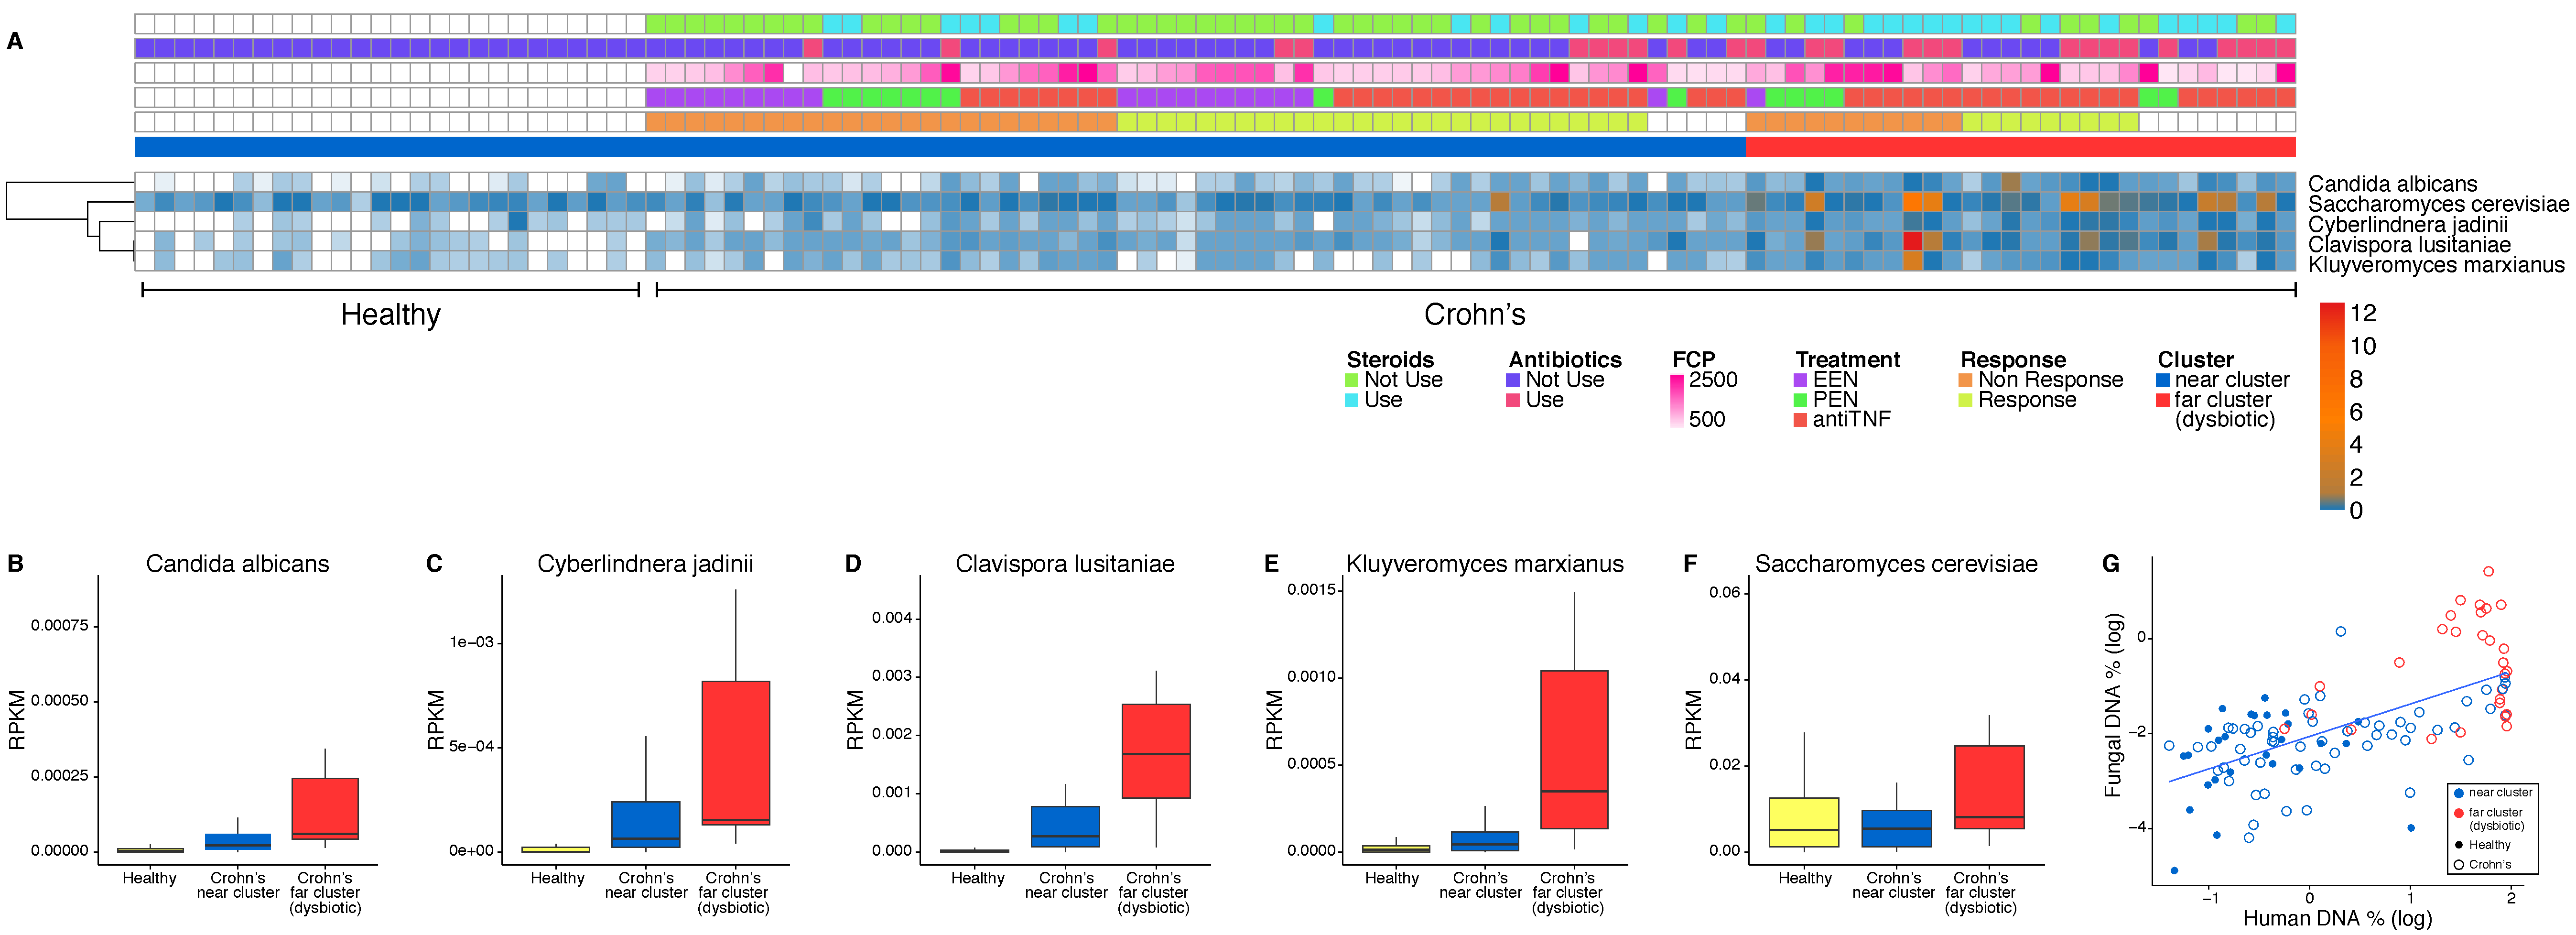
\includegraphics[scale=0.23,trim=0 0 0 0,clip]{Figure/F23_Fugus.pdf}
\caption[Fungal representation in samples from Crohn's disease subjects and healthy controls at baseline]{Fungal representation in samples from Crohn's disease subjects and healthy controls at baseline.
(A) Heatmap summarizing the abundance of fungal taxa present in healthy controls (left side of figure) and children with Crohn's disease (right side of figure). Metadata are indicated by the color code at the top of the figure. White cells indicate missing data.
(B–F) Bar graphs (B)–(F) show the relative abundance of the five main taxa detected. The y axis shows reads per kb of target DNA per million reads in the sample (RPKM).
(G) Graph showing correlation between human DNA \% and fungal DNA \%. Points are colored by membership in the near or far clusters based on the bacterial taxonomic data. Samples from healthy subjects are shown filled and Crohn's disease by open circles. }
\label{F23_Fugus}
\end{sidewaysfigure}




\begin{figure*}[p]
	\centering
	{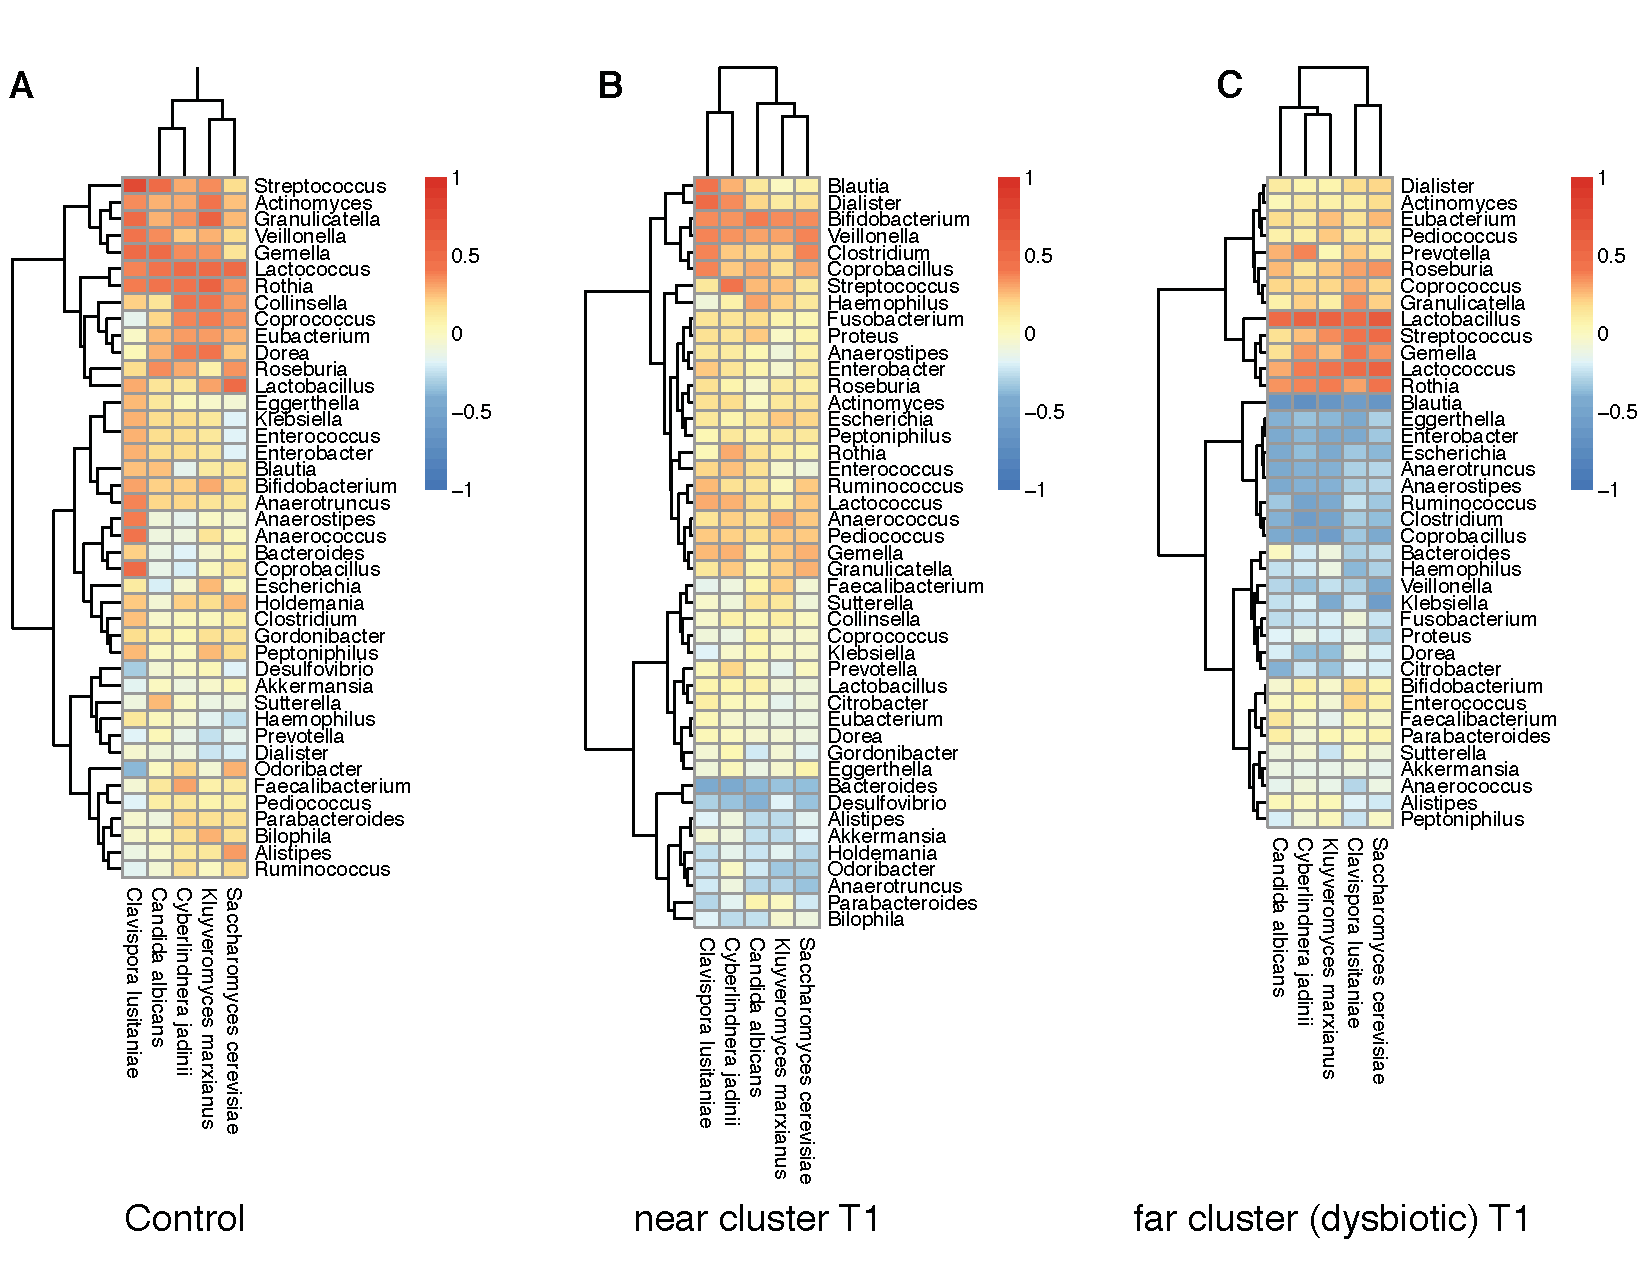
\includegraphics[scale=0.5,trim=0 0 0 0,clip]{Figure/F2S3_taxa_fungi_correlation.pdf}}
	\caption[Correlation of bacterial abundance and fungal abundance at baseline]{Correlation of bacterial abundance and fungal abundance at baseline. Samples studied included A) healthy controls, (B) Crohn’s disease cluster 1 and (C) Crohn’s disease cluster 2. The heat map plots the Spearman correlation for each pair of bacteria and fungi (scale to the right of each panel).
	}
	\label{F2S3_taxa_fungi_correlation}
\end{figure*}



	
\section{Exploring the baseline clusters defined by bacterial abundance in a multivariate model }
We next explored factors associated with membership in the dysbiotic far cluster at baseline (Figure~\ref{Fig21_Microbiome_Cluster_Heatmap}B). In the multivariable model, use of antibiotics within the preceding 6 months, current use of corticosteroids, and abundance of fungi were independently associated with membership in the far cluster. These data indicate that at least part of the previously described dysbiosis in IBD may be due to antibiotic and corticosteroid exposure and that the dysbiosis extends beyond the bacteria to include fungi. 

Given the association with antibiotics, we further defined the bacterial taxa that distinguished Crohn's disease from healthy controls by analyzing only the subset of patients not treated with antibiotics (Table~\ref{TS6}). Separately, we analyzed the association of antibiotic use and taxonomic representation within the Crohn's disease cohort (Table~\ref{TS7}). Bacterial genera associated with Crohn's disease in the absence of antibiotic use were almost completely different from genera associated with antibiotic use in the Crohn's disease cohort (discussed further below). 


\begin{figure*}[p]
\centering
{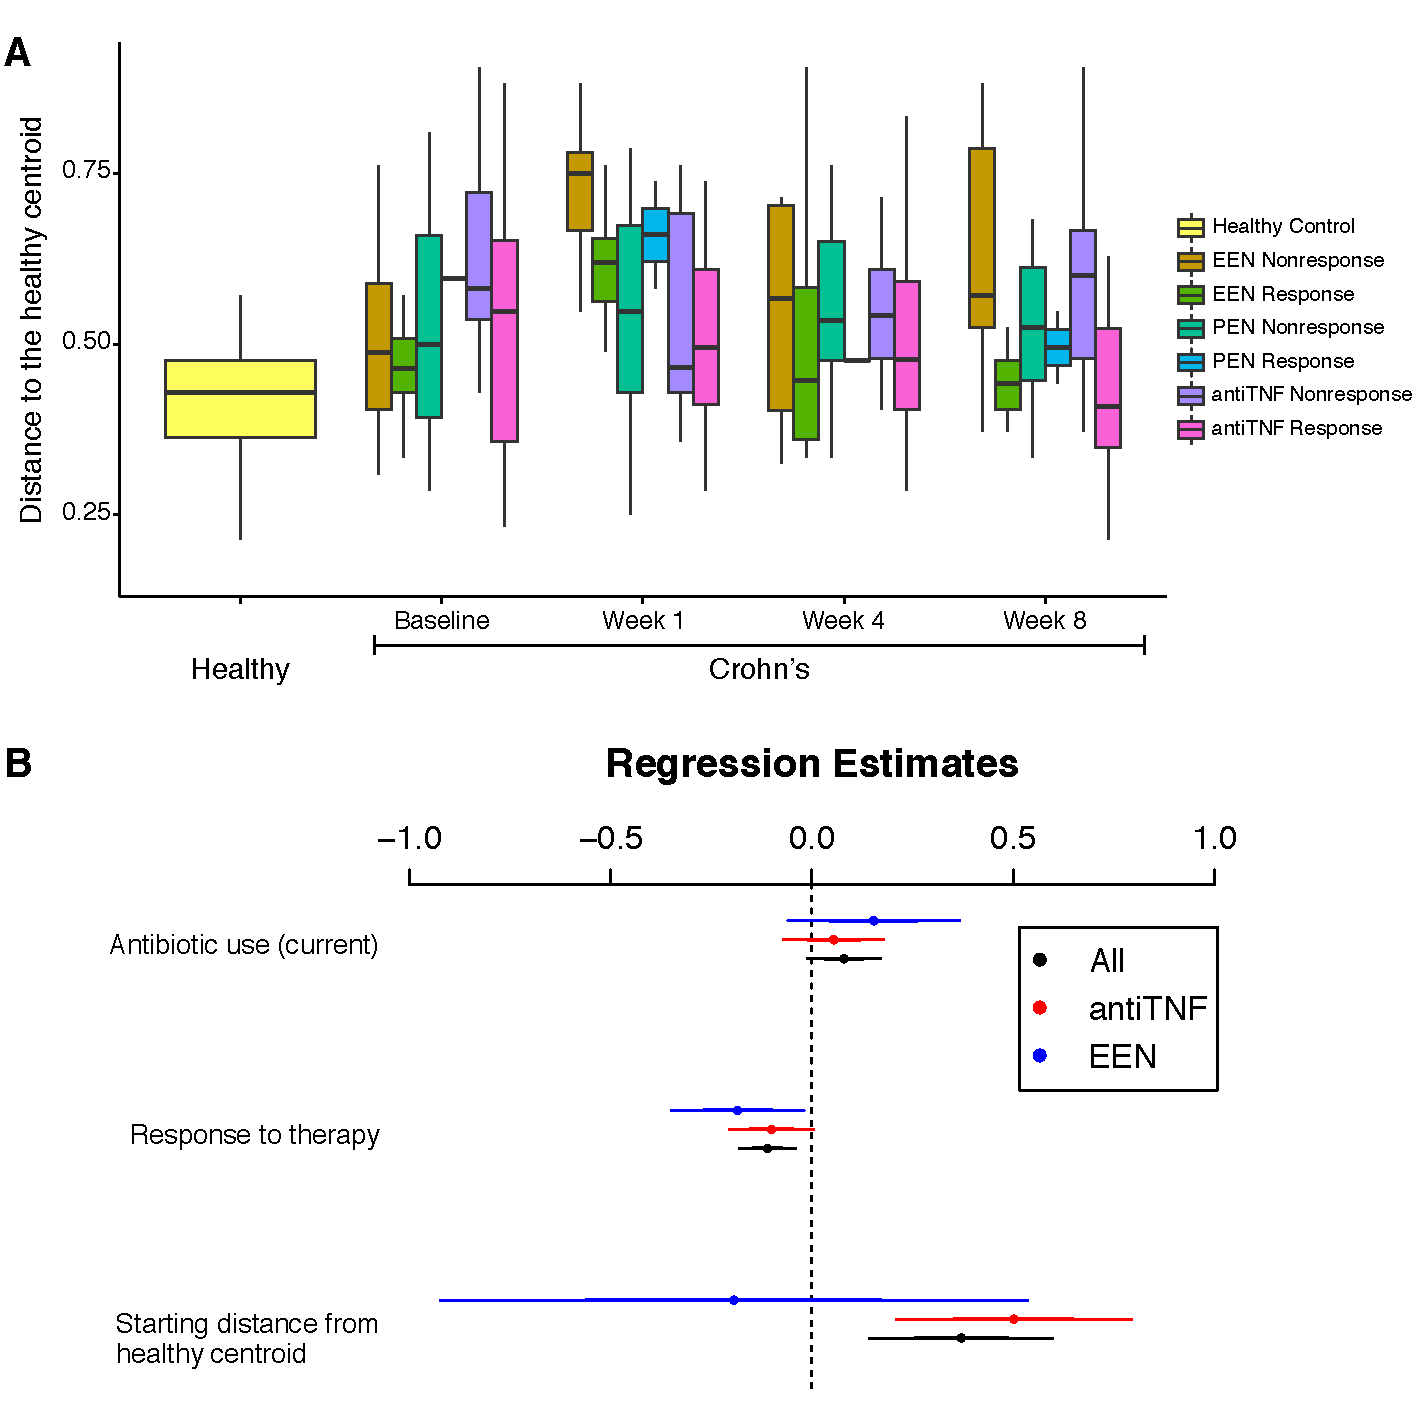
\includegraphics[scale=0.6,trim=0 0 0 0,clip]{Figure/F24_Distance.pdf}}
\caption[Change in the microbiota composition among children with crohn's disease treated with EEN, PEN, and Anti-TNF therapy]{Change in the microbiota composition among children with crohn's disease treated with EEN, PEN, and Anti-TNF therapy.
(A) Characterization of the bacterial taxonomic composition based on distance from the centroid of healthy controls. Boxes show median and first and third quartile. The x axis shows the group and time point, the y axis shows the distance from the centroid of the healthy controls. The groups compared are shown to the right.
(B) Plot of regression coefficients and their confi- dence intervals. The dependent variable used is distance to the healthy centroid. Covariates included antibiotic use, response to therapy defined as reduction in FCP to less than 250 mg/g, and the starting distance from the healthy centroid. Regression coefficients are shown as dots, one SD is shown as the thin lines, and two SDs as the thick lines.
}
\label{F24_Distance}
\end{figure*}




\begin{figure*}[p]
\centering
{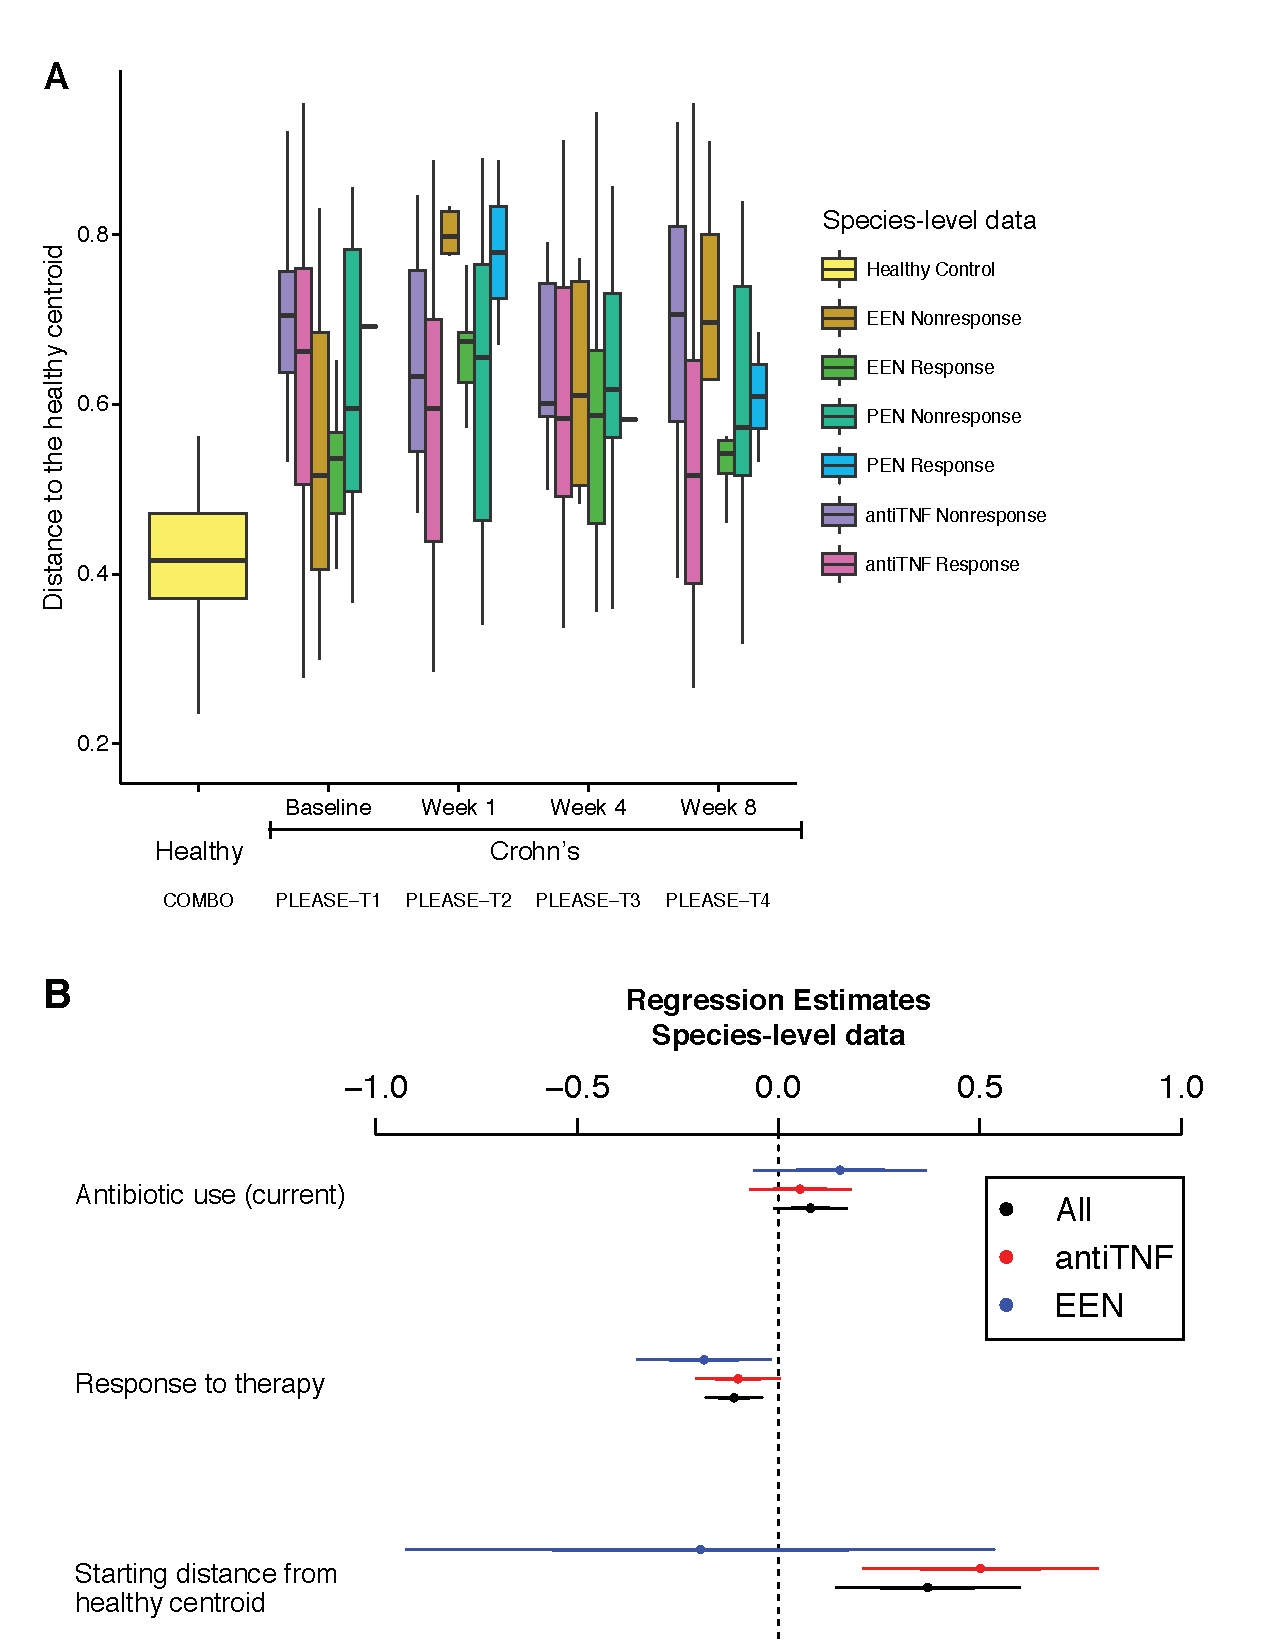
\includegraphics[scale=0.6,trim=0 0 0 0,clip]{Figure/F2S4_distance_species.pdf}}
\caption[Analysis of longitudinal results using species-level data.]{Analysis of longitudinal results using species-level data. A) Analysis based on distance to the centroid of healthy controls. B) Regression analysis of the effects of antibiotics, response, and starting community.
}
\label{F2S4_distance_species}
\end{figure*}



\section{ Clustering did not predict response to therapy }
Rates of response to treatment were not significantly different among patients in the near or far dysbiotic cluster. Twenty-seven patients (53\%) in the near cluster and nine (45\%) patients in the far dysbiotic cluster achieved a reduction in FCP below 250 mg/g (p = 0.60). Among anti-TNF-treated patients the response rates were 66.7\% and 60\%, respectively (p = 0.74). Too few EEN-treated patients were available for meaningful comparison.

\section{ Dynamics of dysbiosis with treatment }
We categorized sequences from each fecal sample by its Jaccard distance from the centroid of the healthy control samples, providing a quantitative measure of dysbiosis, and then analyzed longitudinal dynamics. One of the proposed mechanisms of action of diet-based therapy is to alter the gut microbiota composition. We thus assessed the bacterial composition at baseline and 1 week into therapy (Figure~\ref{F2S4_distance_species}A). The microbiota composition among the EEN-treated group changed within 1 week of therapy, moving significantly farther from centroid of the healthy controls (relative to baseline p = 0.005 overall, p = 0.02 among responders, p = 0.14 among non-responders). One week after initiation of EEN, abundance of 6 of the 40 genera examined were nominally different at a threshold of p = 0.05 (Haemophilus, Alistipes, Streptococcus, Dialister, Dorea, and Gordonibacter; not significant after correction for multiple comparisons; Table~\ref{TS8}). A similar pattern was not seen among the PEN-treated patients (p = 0.83) or anti-TNF-treated patients (p = 0.02, note anti-TNF-treated group moved closer to healthy centroid within 1 week), suggesting that either there is a dose-dependent effect of enteral nutrition or that fully removing regular table food from the diet influences microbiota composition within 1 week. 

We next used linear regression to examine the independent effects of reduction in FCP, antibiotic exposure, and the degree of dysbiosis at baseline on the final state of the microbial community (Figure~\ref{F2S4_distance_species}B). Given the different microbial response to the three therapies during the first week, analyses were conducted combined and stratified by treatment. At the end of the study, responders (i.e., those with reduction in FCP) were closer to the centroid of the healthy controls than nonresponders after adjusting for antibiotic use and initial degree of distance from the centroid (p = 0.003). Similar patterns were seen for anti-TNF therapy (p = 0.06) and EEN (p = 0.06). There were too few responders to PEN for meaningful analysis. Analysis at the species level yielded generally similar results, but with a more pronounced difference in the composition of responders and non-responders to EEN after 1 week of therapy (p = 0.025), a difference that persisted at week 8 (Figures~\ref{F2S4_distance_species}A and \ref{F2S4_distance_species}B). 

The resolution of dysbiosis was not complete among responders. Among the anti-TNF-treated patients who were responders, 11 taxa differed in abundance from healthy controls at baseline (q $<$ 0.05). At the end of follow-up, nine of these taxa (82\%) remained significantly different at a nominal p $<$ 0.05, and six (55\%) were significant at a q $<$ 0.05 (Klebsiella, Prevotella, Escherichia, Odoribacter, Enterococcus, and Fusobacterium). Thus, clinical response was associated with evolution of communities toward healthy structure (Figure~\ref{F2S4_distance_species}B), consistent with the observation that human DNA levels diminished with successful therapy (q = 0.0002; quantile regression), but normal community structure was not usually fully restored (Figure~\ref{F2S4_distance_species}A). This may be due to continuing environmental stress from the host inflammatory response as indicated by mildly elevated FCP despite response to treatment. An analysis at the species level yielded generally similar conclusions (Figures~\ref{F2S4_distance_species}A and \ref{F2S4_distance_species}B). Fungal colonization was not reduced with successful therapy (p = 0.35; quantile regression).

To explore the independent effect of inflammation on the composition of the gut microbiota, we created separate robust quantile (75\%) regression models adjusted for antibiotic use and treatment modality with fold-change in abundance of individual taxa as the dependent variable. Response to therapy defined as final FCP $<$ 250 mg/g was associated with decrease in Actinomyces (p = 0.0002, q = 0.01) and increase in Lactococcus (p = 0.002, q = 0.046) and Roseburia (p = 0.006, q = 0.084). (Table~\ref{TS9}). Multiple gene pathways were also associated with antibiotic use, treatment, and response (Table~\ref{TS10}).

Distinctive responses of genus-level taxa are summarized in Figure~\ref{F25_summary}, which also indicates the time points queried. Specific bacterial lineages showed increases or decreases in abundance associated with (1) health or Crohn's disease at baseline, (2) antibiotic use in the Crohn's disease cohort at baseline, (3) diet therapy in the Crohn's cohort at week 1, and (4) resolution of inflammation (corrected for antibiotic use) in the Crohn's cohort at week 8. 


Distinctive responses were also seen associated with fungal colonization (Figure~\ref{F25_summary}; Table~\ref{TS11}$\sim$\ref{TS14}). At baseline, Candida, Clavispora, Cyberlindnera, and Kluyveromyces were all enriched in Crohn's samples versus healthy controls (Table~\ref{TS11}). Comparisons between antibiotic-treated versus not treated patients showed enrichment of all these fungi plus Saccharomyces as well (Table~\ref{TS12}). In contrast, after one week of diet therapy, Candida, Clavispora, and Cyberlindnera were all reduced in abundance (Table~\ref{TS13}). Similarly, abundance of Clavispora Cyberlindnera, and Kluyveromyces were significantly reduced from baseline to week 8 only in the EEN-treated group (q $<$ 0.05) and not the anti-TNF-treated group. At week 8, overall response to therapy after adjusting for treatment and antibiotic use was not associated with a change in fungal abundance (Table~\ref{TS14}).

\section{ Discussion }
Here we assess the concurrent effects of inflammation, diet, and antibiotic use on the the gut microbiome in pediatric Crohn's disease. The environmental stresses experienced by Crohn's disease patients were associated with changes in microbial taxon- omy that mostly differed among the stressors studied (Figure~\ref{F25_summary}). We observed that patients with Crohn's disease can be categorized into two groups defined by the composition of the bacterial populations, paralleling previous studies based on 16S rRNA gene tag sequencing \citep{Frank:2007hn,gevers2014treatment,Tong:2013bp}. We further showed that dysbiosis involved differences in microbial gene representation, increases in fungal representation, and higher levels of human DNA in stool. Antibiotic exposure, which is common in this population, has also been identified as a risk factor for new onset Crohn's disease \citep{Card:2004tb, Margolis:2010et} and was strongly associated with the dysbiosis observed here. EEN further altered the composition of the gut microbiota, possibly due to elimination of regular table food, despite having a favorable effect on gut inflammation. By our definition, the effect of diet qualifies as dysbiosis, though we note that the changes were distinct from the other stressors studied (Figure~\ref{F25_summary}). Finally, effective therapy with either anti-TNF or EEN reduced, but did not completely eliminate, the dysbiosis present at baseline. Thus, our data demonstrate that diet, antibiotics, and inflammation each independently influence different components of the microbial community. 


\begin{figure*}[p]
\centering
{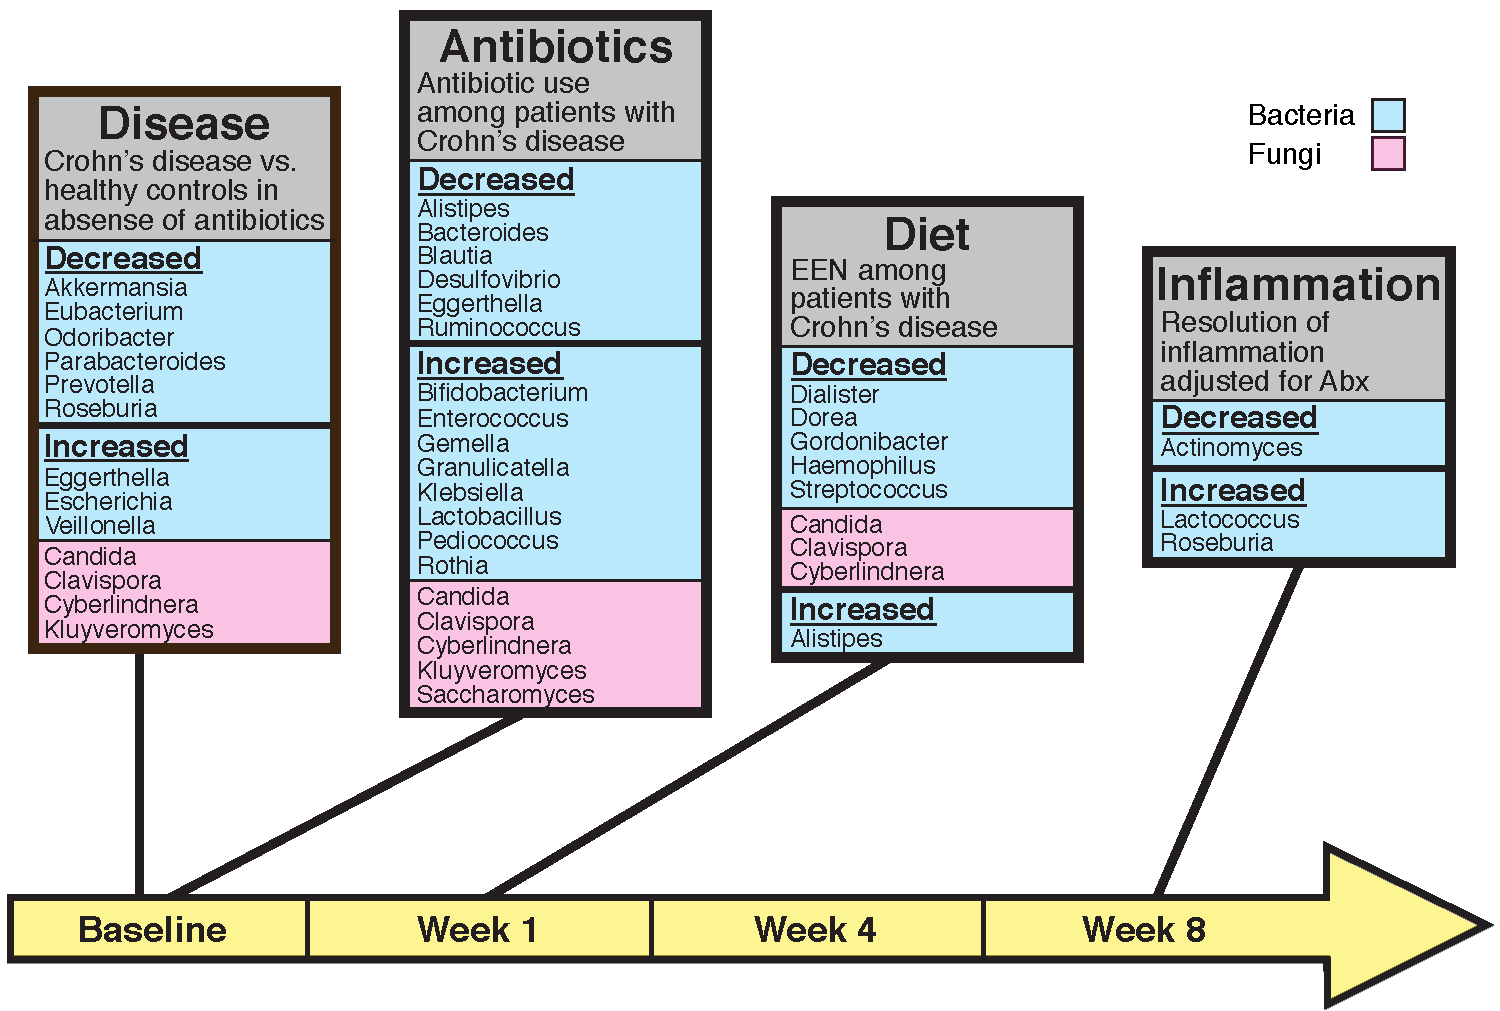
\includegraphics[scale=0.55,trim=0 0 0 0,clip]{Figure/F25_summary.pdf}}
\caption[Bacterial and fungal genera associated with environmental stressors]{Bacterial and fungal genera associated with environmental stressors. Microbial genera are shown that differed in four comparisons: Crohn's disease versus healthy controls at baseline ("Disease"); antibiotic use at baseline in the Crohn's disease cohort ("Antibiotics"); diet (EEN) or anti-TNF therapy at week 1 ("Diet"); and reduction of inflammation or not at the end of the study at week 8 ("Inflammation"). The time line is shown along the bottom (yellow). Baterial lineages are shown in light blue and fungal lineages in pink. Taxa shown were significantly associated after adjustment for multiple comparisons for Crohn’s disease versus healthy controls, for antibiotic use comparisons, and for all fungal comparisons. The bacterial taxa shown for the effect of EEN, and resolution of inflammation were significant at a nominal p value $<$ 0.05 (i.e., without correction for multiple comparisons).

}
\label{F25_summary}
\end{figure*}


We described two clusters of patients based on microbiota composition, though the data can be characterized as either a continuum or a dichotomous grouping. The two clusters were associated with clinical features such as antibiotic use and human DNA but did not appear to predict response to therapy. Thus, the biologic and clinical significance of the clusters remains to be determined.


There were very few taxa whose abundance was associated with more than one stressor. However, the genus Alistipes was increased with EEN but diminished by antibiotic treatment, raising the possibility that antibiotics antagonize the beneficial effects of EEN. 


The independent effects of antibiotics, diet, and inflammation likely reflect different mechanisms. Antibiotics are direct toxins to bacteria and may facilitate outgrowth of fungi. Changes in diet provide novel substrates supporting bacterial growth. Inflammation may select for bacterial taxa able to live in the setting of oxidative stress. The normal oxygen gradient in the colon influences the composition of the gut microbiota with a higher abundance of Proteobacteria in the microaerobic environment of the mucosal surface \citep{Albenberg:2014bp}. Disruption of the epithelium and bleeding due to active Crohn's disease is expected to lead to greater intraluminal oxygen, which in turn would favor outgrowth of taxa belonging to the Proteobacteria phylum. In addition, some Enterobacteriacaea are known to exploit compounds produced during inflammation as terminal electron acceptors, promoting their outgrowth \citep{Winter:2014ed}.


We observed a rapid change in the composition of the gut microbiota within 1 week of initiating EEN, similar to that observed in other small studies of defined formula diets \citep{Gerasimidis:2014gi} and with alterations in whole-food diets \citep{David:2014cl,wu2011linking}. However, this study was unique in the ability to compare PEN to EEN. A similar change in the microbiota was not observed in children receiving PEN, despite administration of nearly the same amount of enteral formula, suggesting that the exclusion of table foods was the primary determinant in changing the gut microbiota and perhaps mediating the increased effectiveness of EEN \citep{lee2015comparative}. After 1 week of EEN, the composition of the microbiota differed between ultimate responders and non-responders, suggesting measures of the microbiota may be used to predict response to therapy. 


Genes from the category "biosynthesis of siderophore group nonribosomal peptides" (Figure~\ref{F22_Pathway_Cluster_Heatmap}A) were more represented in the more dysbiotic far cluster. This may be due to the response of the gut microbiota to blood in the gut lumen, as indicated by the association with human DNA in stool. Siderophores scavenge iron from the environment. Iron has been linked to an invasive phenotype in bacteria, thereby promoting inflammation \citep{Nairz:2010cf}. Thus, blood associated with active IBD may deliver iron to the gut microbiota, promoting dysbiosis. 


The effect of environmental stress on the gut microbiota extends into the Eukaryotic domain. Others have documented increased richness of fungi in patients with Crohn's disease using older methods but have not linked this directly to specific fungi, environmental stressors, or linked changes in the bacterial microbiota \citep{Ott:2008kj, Richard:2015kk}. In a separate study using sequencing of fungal gene tags, we found that Cyberlindnera jadinii (also known as Pichia jadinii or Candida utilis) was proportionally increased in Crohn's patients \citep{Chehoud:2015ga}, confirming the detection of this lineage here. In this study, four of the five fungi detected (Candida, Clavispora, Cyberlindnera, and Kluyveromyces) showed increased representation in Crohn's disease samples at baseline in the absence of antiboitic use. Independently, antibiotic use was also associated with increased colonization by all five fungi. Diet therapy showed the opposite behavior—after 1 week, fungal colonization was diminished (Figure~\ref{F25_summary}). Thus increased fungal colonization is associated independently with disease and antibiotic treatment and diminished with EEN. The reduction with EEN may be a consequence of lower consumption of fungi in food (Saccharomyces and Cyberlindnera are both found in foods), or due to a change in the microbial environment in the gut with EEN, paralleling the change in bacteria. The importance for pathogenesis is unknown, though we note that anti-Saccharomyces antibiodies are used as a biomarker in IBD \citep{Peeters:2001ba, Prideaux:2012kn, Quinton:1998tj}, and fungi have shown to exacerbate colitis in mouse models \citep{Iliev:2012ko}. 

Cyberlindnera and Candida have been positively associated with bacteria including Streptococcus and Lactobacillus. Positive correlation of Candida and Streptococcus has been reported for oral samples from lung transplant recipients \citep{Bittinger:2014hm}, an interaction proposed in medically important mixed biofilms \citep{Metwalli:2013fb}. Possibly antibiotic exposure promotes formation of a mixed community in the inflamed gut, paralleling studies in mice \citep{Dollive:2013cj}. 


The presence of fungi may also have contributed to the metabolic genomic signature associated with IBD (Figures~\ref{F22_Pathway_Cluster_Heatmap}A and \ref{F22_Pathway_Cluster_Heatmap}C). Since bacteria do not have phospholipid membranes as in eukaryotic organisms, it may be that the predominance of genes associated with "glycerolipid metabolism" and "glycerol phospholipid metabolism" (Figure~\ref{F22_Pathway_Cluster_Heatmap}C) in Crohn's disease is due to the abundance of fungi in the dysbiotic far cluster. Indeed, with the exception of actinomycetes group, triacylglycerols in bacteria have rarely been described \citep{Alvarez:2002cy}. These same pathways might also be involved in the catabolism of fatty acid lipids through either peroxisomal or mitochondrial boxidation, again, a feature of eukaryotic organisms like yeast \citep{Strijbis:2010gd} and not bacteria. 


The bacterial microbiota among responders became more similar to the healthy controls than the microbiota of non-responders with both anti-TNF and EEN. Anti-TNF therapy is administered parenterally and is not expected to alter the gut microbiome directly, indicating that dysbiosis is likely a consequence of inflammation. However, the bacterial dysbiosis was only partially resolved among responders, and fungal dysbiosis did not resolve. Perhaps complete resolution would occur with longer follow-up along with a reduction in the stressors to the gut microbiota described here. In turn, complete resolution of bacterial and or fungal dysbiosis might have a favorable impact on Crohn's disease \citep{Rajca:2014bi, Samuel:2010en}.

In conclusion, we document that dysbiosis of Crohn's disease extends beyond bacteria to include fungi. The dysbiosis results from a combination of inflammation, antibiotic exposure, and dietary changes, each exerting different impacts on the gut microbiota composition. EEN caused further departure of the composition of the gut bacteria from the pattern of healthy controls within 1 week, likely due to the elimination of table foods, but was effective in reducing inflammation. The extent of dysbiosis diminished with reduction of inflammation by anti-TNF or EEN, consistent with inflammation contributing directly to the dysbiosis. Gene pathway analysis suggested that the gut microbiota responds to gut environmental stressors through the modification of metabolism. Thus, while dysbiosis in general is common to Crohn's disease, the nature of the dysbiosis is unique to each environmental stressor. Future studies should explore whether these effects interact in ways that influence outcome.







 \newpage
{\footnotesize
\renewcommand{\arraystretch}{0.7} \setlength{\tabcolsep}{3pt}
%\begin{center}
\begin{longtable}{ | r | r | r | r | r | r | r | r | r | r | }
\caption[Metagenomic data sets used in this study]{Metagenomic data sets used in this study.} 
\label{TS1} \\

\hline 
Sample & Subject & Time & Treatment & FCP & Antibiotics & Steroids & Total reads & Human DNA \% & Fungal \%\\
\hline 
\endfirsthead

%\multicolumn{3}{c}%
%{{\bfseries \tablename\ \thetable{} -- continued from previous page}} \\
%\hline \multicolumn{1}{|c|}{\textbf{Time (s)}} &
%\multicolumn{1}{c|}{\textbf{Triple chosen}} &
%\multicolumn{1}{c|}{\textbf{Other feasible triples}} \\ \hline 
%\endhead

%\hline \multicolumn{3}{|r|}{{Continued on next page}} \\ \hline
\endfoot

\hline \hline
\endlastfoot

 
4000 & 4000 & NA & NA & NA & Not.Use & NA & 19515697 & 10.1983 & 0.0001\\ 
4001 & 4001 & NA & NA & NA & Not.Use & NA & 18185930 & 0.5288 & 0.0075\\ 
4002 & 4002 & NA & NA & NA & Not.Use & NA & 27338002 & 0.0985 & 0.0008\\ 
4004 & 4004 & NA & NA & NA & Not.Use & NA & 11092808 & 0.3729 & 0.0036\\ 
4005 & 4005 & NA & NA & NA & Not.Use & NA & 9492196 & 0.6128 & 0.0160\\ 
4006 & 4006 & NA & NA & NA & Not.Use & NA & 23634581 & 1.2993 & 0.0062\\ 
4007 & 4007 & NA & NA & NA & Not.Use & NA & 19368508 & 0.1209 & 0.0001\\ 
4009 & 4009 & NA & NA & NA & Not.Use & NA & 15076205 & 0.5804 & 0.0273\\ 
4010 & 4010 & NA & NA & NA & Not.Use & NA & 15533469 & 3.0424 & 0.0180\\ 
4011 & 4011 & NA & NA & NA & Not.Use & NA & 8136644 & 0.0651 & 0.0002\\ 
4013 & 4013 & NA & NA & NA & Not.Use & NA & 18943086 & 0.0564 & 0.0034\\ 
4014 & 4014 & NA & NA & NA & Not.Use & NA & 15495272 & 0.0458 & 0.0000\\ 
4017 & 4017 & NA & NA & NA & Not.Use & NA & 10603626 & 0.2833 & 0.0243\\ 
4018 & 4018 & NA & NA & NA & Not.Use & NA & 8514099 & 0.2640 & 0.0256\\ 
4019 & 4019 & NA & NA & NA & Not.Use & NA & 36200732 & 0.3610 & 0.0569\\ 
4020 & 4020 & NA & NA & NA & Not.Use & NA & 12334653 & 0.1642 & 0.0015\\ 
4021 & 4021 & NA & NA & NA & Not.Use & NA & 13632049 & 0.0630 & 0.0035\\ 
4022 & 4022 & NA & NA & NA & Not.Use & NA & 13206400 & 0.1255 & 0.0073\\ 
4023 & 4023 & NA & NA & NA & Not.Use & NA & 15064745 & 0.1460 & 0.0087\\ 
4024 & 4024 & NA & NA & NA & Not.Use & NA & 9780269 & 0.3793 & 0.0245\\ 
4025 & 4025 & NA & NA & NA & Not.Use & NA & 12662584 & 0.1160 & 0.0011\\ 
4026 & 4026 & NA & NA & NA & Not.Use & NA & 12604291 & 0.0992 & 0.0127\\ 
4027 & 4027 & NA & NA & NA & Not.Use & NA & 214239 & 0.7977 & 0.0019\\ 
4028 & 4028 & NA & NA & NA & Not.Use & NA & 6426484 & 0.1371 & 0.0338\\ 
4029 & 4029 & NA & NA & NA & Not.Use & NA & 11631985 & 0.4315 & 0.0023\\ 
4030 & 4030 & NA & NA & NA & Not.Use & NA & 14506623 & 2.3105 & 0.0062\\ 
5001-01 & 5001 & 1 & antiTNF & 2137 & Not.Use & Not.Use & 11599370 & 91.0922 & 0.2073\\ 
5001-02 & 5001 & 2 & antiTNF & 607 & Not.Use & Not.Use & 12641013 & 89.3180 & 0.0709\\ 
5001-03 & 5001 & 3 & antiTNF & 867 & Not.Use & Not.Use & 13630280 & 19.6892 & 0.0122\\ 
5001-04 & 5001 & 4 & antiTNF & 557 & Not.Use & Not.Use & 14353075 & 0.8513 & 1.2650\\ 
5002-01 & 5002 & 1 & antiTNF & 2178 & Not.Use & Use & 10400185 & 27.6042 & 0.0135\\ 
5002-02 & 5002 & 2 & antiTNF & 950 & Not.Use & Use & 14497980 & 17.0893 & 0.0105\\ 
5002-03 & 5002 & 3 & antiTNF & 1947 & Not.Use & Use & 16679087 & 88.5445 & 0.0667\\ 
5002-04 & 5002 & 4 & antiTNF & 1880 & Not.Use & Use & 5804379 & 89.5499 & 0.0567\\ 
5003-01 & 5003 & 1 & antiTNF & 1854 & Not.Use & Not.Use & 7241664 & 0.4341 & 0.0085\\ 
5003-02 & 5003 & 2 & antiTNF & 1177 & Not.Use & Not.Use & 10238790 & 4.7584 & 0.0247\\ 
5003-03 & 5003 & 3 & antiTNF & 282 & Not.Use & Not.Use & 12894252 & 0.2021 & 0.0045\\ 
5003-04 & 5003 & 4 & antiTNF & 46 & Not.Use & Not.Use & 14189310 & 0.7290 & 0.0115\\ 
5004-01 & 5004 & 1 & PEN & 1625 & Not.Use & Not.Use & 14242923 & 31.4914 & 0.0106\\ 
5004-02 & 5004 & 2 & PEN & 161 & Not.Use & Not.Use & 9820090 & 0.2262 & 0.0140\\ 
5004-03 & 5004 & 3 & PEN & 1458 & Not.Use & Not.Use & 12543255 & 21.1037 & 0.0090\\ 
5004-04 & 5004 & 4 & PEN & 981 & Not.Use & Not.Use & 16618938 & 0.4540 & 0.0114\\ 
5005-01 & 5005 & 1 & antiTNF & 1896 & Not.Use & Not.Use & NA & NA & NA\\ 
5005-02 & 5005 & 2 & antiTNF & 1800 & Not.Use & Not.Use & NA & NA & NA\\ 
5005-03 & 5005 & 3 & antiTNF & 929 & Not.Use & Not.Use & NA & NA & NA\\ 
5005-04 & 5005 & 4 & antiTNF & NA & NA & Not.Use & NA & NA & NA\\ 
5006-01 & 5006 & 1 & antiTNF & 343 & Not.Use & Not.Use & 17243968 & 0.0406 & 0.0056\\ 
5006-02 & 5006 & 2 & antiTNF & 970 & Not.Use & Not.Use & 3911681 & 0.0669 & 0.0051\\ 
5006-03 & 5006 & 3 & antiTNF & 280 & Not.Use & Not.Use & 13509151 & 0.1451 & 0.0164\\ 
5006-04 & 5006 & 4 & antiTNF & 144 & Not.Use & Not.Use & 15656896 & 0.0257 & 0.0044\\ 
5007-01 & 5007 & 1 & antiTNF & 1374 & Use & Not.Use & 7042144 & 12.3010 & 0.0283\\ 
5007-02 & 5007 & 2 & antiTNF & 213 & Use & Not.Use & 6026836 & 0.7321 & 0.0116\\ 
5007-03 & 5007 & 3 & antiTNF & 228 & Not.Use & Not.Use & 20253427 & 1.3537 & 0.0079\\ 
5007-04 & 5007 & 4 & antiTNF & 631 & Not.Use & Not.Use & 2934904 & 1.5784 & 0.0437\\ 
5008-01 & 5008 & 1 & PEN & 852 & Not.Use & Not.Use & 16003947 & 0.0782 & 0.0052\\ 
5008-02 & 5008 & 2 & PEN & 338 & Not.Use & Not.Use & 8817907 & 0.2731 & 0.0065\\ 
5008-03 & 5008 & 3 & PEN & 332 & Not.Use & Not.Use & 1486829 & 0.5910 & 0.0080\\ 
5008-04 & 5008 & 4 & PEN & NA & Not.Use & Not.Use & 1400790 & 0.5865 & 0.0504\\ 
5010-01 & 5010 & 1 & antiTNF & 1311 & Not.Use & Not.Use & 9617274 & 0.4466 & 0.0067\\ 
5010-02 & 5010 & 2 & antiTNF & 1325 & Not.Use & Not.Use & 1104 & 8.1522 & 0.3945\\ 
5010-03 & 5010 & 3 & antiTNF & 279 & Not.Use & Not.Use & 16091975 & 0.1894 & 0.0065\\ 
5010-04 & 5010 & 4 & antiTNF & 412 & Not.Use & Not.Use & 4913506 & 0.6266 & 0.0127\\ 
5011-01 & 5011 & 1 & PEN & 2144 & Use & Use & 29237981 & 77.0695 & 0.0447\\ 
5011-02 & 5011 & 2 & PEN & 1598 & Use & Use & 20544281 & 53.1918 & 0.0198\\ 
5011-03 & 5011 & 3 & PEN & 482 & Use & Use & 10625712 & 1.8862 & 0.0440\\ 
5011-04 & 5011 & 4 & PEN & 1041 & Use & Use & 10947858 & 0.5956 & 0.0089\\ 
5012-01 & 5012 & 1 & PEN & 461 & Not.Use & Use & 9663238 & 16.2560 & 0.0078\\ 
5012-02 & 5012 & 2 & PEN & 1125 & Not.Use & Use & 3831035 & 0.2822 & 0.0063\\ 
5012-03 & 5012 & 3 & PEN & 2500 & Not.Use & Use & 4837908 & 1.4325 & 0.0088\\ 
5012-04 & 5012 & 4 & PEN & 1129 & Not.Use & Use & 6070173 & 3.2714 & 0.0089\\ 
5013-01 & 5013 & 1 & PEN & 1504 & Not.Use & Not.Use & 8697517 & 0.8142 & 0.0053\\ 
5013-02 & 5013 & 2 & PEN & 372 & Not.Use & Not.Use & 6674500 & 0.1513 & 0.0059\\ 
5013-03 & 5013 & 3 & PEN & 747 & Not.Use & Not.Use & 9299951 & 0.0331 & 0.0062\\ 
5013-04 & 5013 & 4 & PEN & 743 & Not.Use & Not.Use & 12734738 & 0.0226 & 0.0056\\ 
5015-01 & 5015 & 1 & antiTNF & 392 & Use & Use & 7228455 & 0.1064 & 0.0054\\ 
5015-02 & 5015 & 2 & antiTNF & 80 & Use & Use & 6843728 & 0.0121 & 0.0087\\ 
5015-03 & 5015 & 3 & antiTNF & 24 & Use & Use & 7573849 & 0.0220 & 0.0057\\ 
5015-04 & 5015 & 4 & antiTNF & 26 & Use & Use & 8469678 & 0.0231 & 0.0047\\ 
5016-01 & 5016 & 1 & antiTNF & 399 & Use & Use & 2283485 & 59.8309 & 26.6041\\ 
5016-02 & 5016 & 2 & antiTNF & 236 & Use & Use & 3260627 & 22.8888 & 1.3035\\ 
5016-03 & 5016 & 3 & antiTNF & 227 & Use & Use & 4810979 & 0.8761 & 0.0631\\ 
5016-04 & 5016 & 4 & antiTNF & 334 & Not.Use & Use & 6652415 & 0.2547 & 0.0188\\ 
5017-01 & 5017 & 1 & PEN & 379 & Not.Use & Use & 10287120 & 3.7480 & 0.0056\\ 
5017-02 & 5017 & 2 & PEN & 238 & Not.Use & Use & 4845144 & 0.5478 & 0.0073\\ 
5017-03 & 5017 & 3 & PEN & 701 & Not.Use & Use & 6308649 & 0.0573 & 0.0092\\ 
5017-04 & 5017 & 4 & PEN & 690 & Not.Use & Use & 3322423 & 0.1149 & 0.0052\\ 
5018-01 & 5018 & 1 & PEN & 379 & Not.Use & Use & 8195134 & 0.4385 & 0.0109\\ 
5018-02 & 5018 & 2 & PEN & 397 & Not.Use & Use & 58536 & 2.7744 & 0.1933\\ 
5018-03 & 5018 & 3 & PEN & 410 & Not.Use & Use & 6121 & 0.3267 & 0.0983\\ 
5018-04 & 5018 & 4 & PEN & 195 & Not.Use & Use & 12808694 & 0.0201 & 0.0050\\ 
5020-01 & 5020 & 1 & PEN & 47 & Use & Use & 1618940 & 7.7967 & 0.3189\\ 
5020-02 & 5020 & 2 & PEN & 70 & Use & Use & 5165378 & 2.3365 & 0.0175\\ 
5020-03 & 5020 & 3 & PEN & 93 & Use & Use & 7124673 & 1.4249 & 0.0085\\ 
5020-04 & 5020 & 4 & PEN & 110 & Use & Use & 13534664 & 0.0486 & 0.0070\\ 
5022-01 & 5022 & 1 & antiTNF & 1040 & Use & Not.Use & 11047813 & 6.5517 & 0.0096\\ 
5022-02 & 5022 & 2 & antiTNF & 653 & Use & Not.Use & 6130429 & 1.5631 & 0.0083\\ 
5022-03 & 5022 & 3 & antiTNF & 148 & Use & Not.Use & 8780435 & 0.2941 & 0.0081\\ 
5022-04 & 5022 & 4 & antiTNF & 48 & Not.Use & Not.Use & 17211378 & 0.3548 & 0.0654\\ 
5023-01 & 5023 & 1 & antiTNF & 921 & Use & Not.Use & 14356771 & 18.6317 & 0.0120\\ 
5023-02 & 5023 & 2 & antiTNF & 218 & Use & Not.Use & 11397519 & 14.6218 & 0.0385\\ 
5023-03 & 5023 & 3 & antiTNF & 323 & Not.Use & Not.Use & 5671261 & 0.9377 & 0.0186\\ 
5023-04 & 5023 & 4 & antiTNF & 180 & Not.Use & Not.Use & 2679 & 27.0623 & 0.3071\\ 
5025-01 & 5025 & 1 & PEN & NA & Not.Use & Use & NA & NA & NA\\ 
5025-02 & 5025 & 2 & PEN & 457 & Not.Use & Use & 11367288 & 20.5615 & 0.0503\\ 
5025-03 & 5025 & 3 & PEN & 816 & Not.Use & Use & 14894699 & 0.5286 & 0.0756\\ 
5025-04 & 5025 & 4 & PEN & 54 & Not.Use & Use & 7218406 & 0.6819 & 0.0486\\ 
5026-01 & 5026 & 1 & PEN & 961 & Use & Use & 6084502 & 56.7901 & 4.3948\\ 
5026-02 & 5026 & 2 & PEN & 722 & Use & Use & 5818626 & 61.4567 & 0.2509\\ 
5026-03 & 5026 & 3 & PEN & 567 & Use & Use & 8259927 & 30.0102 & 0.1687\\ 
5026-04 & 5026 & 4 & PEN & 365 & Use & Use & 13642402 & 12.7829 & 0.1496\\ 
5027-01 & 5027 & 1 & PEN & 611 & Not.Use & Not.Use & 7596126 & 0.1742 & 0.0128\\ 
5027-02 & 5027 & 2 & PEN & 716 & Not.Use & Not.Use & 8760843 & 0.1641 & 0.0115\\ 
5027-03 & 5027 & 3 & PEN & 466 & Not.Use & Not.Use & 20195710 & 0.2285 & 0.0132\\ 
5027-04 & 5027 & 4 & PEN & 375 & Not.Use & Not.Use & 14403318 & 0.1000 & 0.0121\\ 
5029-01 & 5029 & 1 & antiTNF & 903 & Not.Use & Not.Use & 6004698 & 36.3167 & 0.0483\\ 
5029-02 & 5029 & 2 & antiTNF & 636 & Not.Use & Not.Use & 12741808 & 42.6572 & 0.0299\\ 
5029-03 & 5029 & 3 & antiTNF & 568 & Not.Use & Not.Use & 10820369 & 5.3879 & 0.0732\\ 
5029-04 & 5029 & 4 & antiTNF & 486 & Not.Use & Not.Use & 8918719 & 6.7019 & 0.0391\\ 
5030-01 & 5030 & 1 & antiTNF & 1445 & Not.Use & Not.Use & 8822474 & 86.7239 & 0.1535\\ 
5030-02 & 5030 & 2 & antiTNF & 839 & Not.Use & Not.Use & 13296995 & 2.5554 & 0.0163\\ 
5030-03 & 5030 & 3 & antiTNF & 631 & Not.Use & Not.Use & 8922602 & 54.5344 & 0.2972\\ 
5030-04 & 5030 & 4 & antiTNF & 876 & Not.Use & Not.Use & 9837970 & 10.0054 & 0.0263\\ 
5031-01 & 5031 & 1 & antiTNF & 317 & Use & Not.Use & 20889887 & 79.6034 & 5.2561\\ 
5031-02 & 5031 & 2 & antiTNF & 52 & Use & Not.Use & 25968202 & 9.8291 & 0.3473\\ 
5031-03 & 5031 & 3 & antiTNF & 27 & Use & Not.Use & 6151211 & 31.2159 & 2.0652\\ 
5031-04 & 5031 & 4 & antiTNF & 21 & Use & Not.Use & 4138618 & 20.7082 & 4.4073\\ 
5032-01 & 5032 & 1 & antiTNF & 813 & Not.Use & Not.Use & 2614389 & 86.9049 & 0.1852\\ 
5032-02 & 5032 & 2 & antiTNF & 298 & Not.Use & Not.Use & 3406304 & 70.2177 & 0.0664\\ 
5032-03 & 5032 & 3 & antiTNF & 206 & Not.Use & Not.Use & 6892374 & 89.1729 & 0.1935\\ 
5032-04 & 5032 & 4 & antiTNF & 64 & Not.Use & Not.Use & 18328030 & 0.1624 & 0.0124\\ 
5033-01 & 5033 & 1 & antiTNF & 127 & Not.Use & Not.Use & 6865676 & 4.9233 & 0.0148\\ 
5033-02 & 5033 & 2 & antiTNF & 297 & Not.Use & Not.Use & 19437578 & 0.6928 & 0.0120\\ 
5033-03 & 5033 & 3 & antiTNF & 140 & Not.Use & Not.Use & 7528435 & 0.3262 & 0.0184\\ 
5033-04 & 5033 & 4 & antiTNF & 370 & Not.Use & Not.Use & 9213794 & 0.3658 & 0.0168\\ 
5034-01 & 5034 & 1 & antiTNF & 2500 & Not.Use & Use & 3285312 & 0.1570 & 0.0133\\ 
5034-02 & 5034 & 2 & antiTNF & 494 & Not.Use & Use & 4036397 & 1.7559 & 0.0163\\ 
5034-03 & 5034 & 3 & antiTNF & 2165 & Not.Use & Use & 2297587 & 2.8352 & 0.6844\\ 
5034-04 & 5034 & 4 & antiTNF & 2284 & Not.Use & Use & 5025640 & 75.9482 & 0.0943\\ 
5035-01 & 5035 & 1 & antiTNF & 47 & Use & Not.Use & NA & NA & NA\\ 
5035-02 & 5035 & 2 & antiTNF & 28 & Use & Not.Use & NA & NA & NA\\ 
5035-03 & 5035 & 3 & antiTNF & 20 & Use & Not.Use & NA & NA & NA\\ 
5035-04 & 5035 & 4 & antiTNF & 52 & Use & Not.Use & NA & NA & NA\\ 
5037-01 & 5037 & 1 & PEN & 492 & Not.Use & Not.Use & 74582008 & 7.9909 & 0.0176\\ 
5037-02 & 5037 & 2 & PEN & 2212 & Not.Use & Not.Use & 34438194 & 0.5440 & 0.0183\\ 
5037-03 & 5037 & 3 & PEN & 1014 & Not.Use & Not.Use & 1790636 & 0.3056 & 0.0202\\ 
5037-04 & 5037 & 4 & PEN & 822 & Not.Use & Not.Use & 2152559 & 0.1268 & 0.0137\\ 
5039-01 & 5039 & 1 & PEN & 2500 & Not.Use & Not.Use & 2029437 & 83.5586 & 0.3165\\ 
5039-02 & 5039 & 2 & PEN & 1521 & Not.Use & Not.Use & 8908497 & 72.2014 & 0.0429\\ 
5039-03 & 5039 & 3 & PEN & 1475 & Not.Use & Not.Use & 1962014 & 3.6575 & 0.0187\\ 
5039-04 & 5039 & 4 & PEN & NA & Not.Use & Not.Use & 1029173 & 2.4329 & 0.2934\\ 
5040-01 & 5040 & 1 & antiTNF & 294 & Not.Use & Not.Use & 28075241 & 0.1237 & 0.0017\\ 
5040-02 & 5040 & 2 & antiTNF & 92 & Not.Use & Not.Use & 15463789 & 0.5265 & 0.0224\\ 
5040-03 & 5040 & 3 & antiTNF & 42 & Not.Use & Not.Use & 10911644 & 0.7900 & 0.0819\\ 
5040-04 & 5040 & 4 & antiTNF & 30 & Not.Use & Not.Use & 9808942 & 0.2869 & 0.0262\\ 
5041-01 & 5041 & 1 & antiTNF & 307 & Not.Use & Not.Use & 15150699 & 4.6220 & 0.0094\\ 
5041-02 & 5041 & 2 & antiTNF & 185 & Not.Use & Not.Use & 12355021 & 0.5391 & 0.0003\\ 
5041-03 & 5041 & 3 & antiTNF & 136 & Not.Use & Not.Use & 13562938 & 33.6441 & 0.0087\\ 
5041-04 & 5041 & 4 & antiTNF & 17 & Not.Use & Not.Use & 11522308 & 6.3358 & 0.2214\\ 
5042-01 & 5042 & 1 & antiTNF & 342 & Not.Use & Not.Use & 22535561 & 0.2947 & 0.0005\\ 
5042-02 & 5042 & 2 & antiTNF & 182 & Not.Use & Not.Use & 11828781 & 0.2123 & 0.0022\\ 
5042-03 & 5042 & 3 & antiTNF & 190 & Not.Use & Not.Use & 16371967 & 0.0390 & 0.0004\\ 
5042-04 & 5042 & 4 & antiTNF & 29 & Not.Use & Not.Use & 11444636 & 0.5479 & 0.0068\\ 
5043-01 & 5043 & 1 & PEN & 2400 & Use & Use & 11964783 & 87.5406 & 0.0244\\ 
5043-02 & 5043 & 2 & PEN & 1159 & Use & Use & 682256 & 26.6627 & 0.0751\\ 
5043-03 & 5043 & 3 & PEN & 655 & Not.Use & Use & 19269838 & 0.1763 & 0.0004\\ 
5043-04 & 5043 & 4 & PEN & 500 & Not.Use & Use & 36696745 & 0.4341 & 0.0088\\ 
5044-01 & 5044 & 1 & antiTNF & 254 & Not.Use & Use & 9340353 & 0.8946 & 0.0527\\ 
5044-02 & 5044 & 2 & antiTNF & 479 & Not.Use & Use & 10116721 & 0.7430 & 0.0633\\ 
5044-03 & 5044 & 3 & antiTNF & 354 & Not.Use & Use & 4316774 & 13.8935 & 0.5917\\ 
5044-04 & 5044 & 4 & antiTNF & 475 & Not.Use & Use & 154750 & 2.3444 & 0.0093\\ 
5045-01 & 5045 & 1 & antiTNF & 188 & Use & Not.Use & 17228967 & 0.1411 & 0.0019\\ 
5045-02 & 5045 & 2 & antiTNF & 27 & Use & Not.Use & 12522717 & 0.0783 & 0.0010\\ 
5045-03 & 5045 & 3 & antiTNF & 71 & Use & Not.Use & 16362609 & 0.1187 & 0.0007\\ 
5045-04 & 5045 & 4 & antiTNF & 56 & Use & Not.Use & 10725574 & 0.2865 & 0.0030\\ 
5046-01 & 5046 & 1 & antiTNF & 175 & Not.Use & Use & 13963765 & 0.2269 & 0.0027\\ 
5046-02 & 5046 & 2 & antiTNF & 222 & Not.Use & Use & 10613814 & 0.4613 & 0.0374\\ 
5046-03 & 5046 & 3 & antiTNF & 134 & Not.Use & Use & 9441992 & 0.7746 & 0.0123\\ 
5046-04 & 5046 & 4 & antiTNF & 100 & Not.Use & Use & 1783759 & 4.0816 & 0.1862\\ 
5047-01 & 5047 & 1 & antiTNF & 273 & Not.Use & Use & 10439441 & 2.5958 & 0.0121\\ 
5047-02 & 5047 & 2 & antiTNF & 183 & Not.Use & Use & 11830819 & 1.0136 & 0.0150\\ 
5047-03 & 5047 & 3 & antiTNF & 117 & Not.Use & Use & 17854757 & 1.0251 & 0.0108\\ 
5047-04 & 5047 & 4 & antiTNF & 117 & Not.Use & Use & 12678606 & 1.7812 & 0.0142\\ 
5048-01 & 5048 & 1 & antiTNF & 2500 & Use & Use & 26280822 & 62.4157 & 0.0334\\ 
5048-02 & 5048 & 2 & antiTNF & 742 & Use & Use & 12088681 & 1.8644 & 0.0273\\ 
5048-03 & 5048 & 3 & antiTNF & 135 & Use & Use & 13577418 & 40.8145 & 0.0123\\ 
5048-04 & 5048 & 4 & antiTNF & 54 & Use & Use & 8808904 & 3.1827 & 0.1859\\ 
5049-01 & 5049 & 1 & antiTNF & 2500 & Use & Use & 19127324 & 90.2792 & 0.0255\\ 
5049-02 & 5049 & 2 & antiTNF & 643 & Use & Use & 9370287 & 26.8775 & 0.1222\\ 
5049-03 & 5049 & 3 & antiTNF & 1358 & Use & Use & 15969824 & 81.9447 & 1.8719\\ 
5049-04 & 5049 & 4 & antiTNF & 16 & Use & Use & 18801031 & 90.8234 & 0.0325\\ 
5050-01 & 5050 & 1 & antiTNF & 475 & Not.Use & Not.Use & 16382545 & 0.3588 & 0.0005\\ 
5050-02 & 5050 & 2 & antiTNF & 979 & Not.Use & Not.Use & 20773901 & 0.3808 & 0.0012\\ 
5050-03 & 5050 & 3 & antiTNF & 448 & Not.Use & Not.Use & 15406882 & 0.2307 & 0.0034\\ 
5050-04 & 5050 & 4 & antiTNF & 16 & Not.Use & Not.Use & 11691584 & 4.9108 & 0.0013\\ 
5051-01 & 5051 & 1 & antiTNF & 580 & Use & Not.Use & NA & NA & NA\\ 
5051-02 & 5051 & 2 & antiTNF & 668 & Use & Not.Use & NA & NA & NA\\ 
5051-03 & 5051 & 3 & antiTNF & NA & NA & Not.Use & NA & NA & NA\\ 
5051-04 & 5051 & 4 & antiTNF & NA & NA & Not.Use & NA & NA & NA\\ 
5052-01 & 5052 & 1 & antiTNF & 1160 & Not.Use & Not.Use & 10729210 & 1.7819 & 0.0039\\ 
5052-02 & 5052 & 2 & antiTNF & 308 & Not.Use & Not.Use & 12617073 & 0.8202 & 0.0427\\ 
5052-03 & 5052 & 3 & antiTNF & 150 & Not.Use & Not.Use & 11124443 & 1.1617 & 0.0185\\ 
5052-04 & 5052 & 4 & antiTNF & 168 & Not.Use & Not.Use & 8205232 & 0.2485 & 0.0059\\ 
5053-01 & 5053 & 1 & antiTNF & 48 & Use & Not.Use & 11655187 & 0.5663 & 0.0127\\ 
5053-02 & 5053 & 2 & antiTNF & 23 & Use & Not.Use & 1556543 & 3.2316 & 0.0767\\ 
5053-03 & 5053 & 3 & antiTNF & 38 & Use & Not.Use & 951941 & 17.6339 & 1.0188\\ 
5053-04 & 5053 & 4 & antiTNF & 19 & Use & Not.Use & 17667128 & 13.3496 & 0.0324\\ 
5054-01 & 5054 & 1 & antiTNF & 1368 & Use & Use & 20599524 & 77.2987 & 0.0532\\ 
5054-02 & 5054 & 2 & antiTNF & 1078 & Use & Use & 10007742 & 52.2793 & 0.0239\\ 
5054-03 & 5054 & 3 & antiTNF & 193 & Use & Use & 4333465 & 48.7428 & 0.7540\\ 
5054-04 & 5054 & 4 & antiTNF & 490 & Use & Use & 25145577 & 73.6434 & 0.2921\\ 
5055-01 & 5055 & 1 & antiTNF & 368 & Use & Not.Use & 8681705 & 49.0373 & 5.2491\\ 
5055-02 & 5055 & 2 & antiTNF & 73 & Use & Not.Use & 9604775 & 18.3173 & 5.0463\\ 
5055-03 & 5055 & 3 & antiTNF & 38 & Use & Not.Use & 3292776 & 35.3810 & 4.1493\\ 
5055-04 & 5055 & 4 & antiTNF & 39 & Not.Use & Not.Use & 8298968 & 1.7126 & 0.1305\\ 
5056-01 & 5056 & 1 & antiTNF & 283 & Not.Use & Not.Use & 7468825 & 0.9790 & 0.0268\\ 
5056-02 & 5056 & 2 & antiTNF & 129 & Not.Use & Not.Use & 8007527 & 0.4084 & 0.0303\\ 
5056-03 & 5056 & 3 & antiTNF & 17 & Not.Use & Not.Use & 10081004 & 0.6913 & 0.0454\\ 
5056-04 & 5056 & 4 & antiTNF & 16 & Not.Use & Not.Use & 7765830 & 0.9182 & 0.0567\\ 
5057-01 & 5057 & 1 & antiTNF & 519 & Not.Use & Use & 10010582 & 50.2020 & 3.6336\\ 
5057-02 & 5057 & 2 & antiTNF & 224 & Not.Use & Use & 14875277 & 2.0396 & 0.0241\\ 
5057-03 & 5057 & 3 & antiTNF & 231 & Use & Use & 4960112 & 36.0512 & 0.8362\\ 
5057-04 & 5057 & 4 & antiTNF & 363 & Use & Use & 7121858 & 27.9359 & 1.6837\\ 
5058-01 & 5058 & 1 & antiTNF & 836 & Not.Use & Use & 8585750 & 0.3260 & 0.0025\\ 
5058-02 & 5058 & 2 & antiTNF & 877 & Not.Use & Use & 8512412 & 0.6551 & 0.0172\\ 
5058-03 & 5058 & 3 & antiTNF & 466 & Not.Use & Use & 12885140 & 0.8309 & 0.0019\\ 
5058-04 & 5058 & 4 & antiTNF & 123 & Not.Use & Use & 12382956 & 5.0393 & 0.0079\\ 
5060-01 & 5060 & 1 & antiTNF & 425 & Use & Use & 4288336 & 52.0995 & 1.1957\\ 
5060-02 & 5060 & 2 & antiTNF & 78 & Use & Use & 9491463 & 20.7642 & 0.6907\\ 
5060-03 & 5060 & 3 & antiTNF & 130 & Not.Use & Use & 7310082 & 8.9870 & 0.0919\\ 
5060-04 & 5060 & 4 & antiTNF & 121 & Not.Use & Use & 10794119 & 28.4916 & 0.1761\\ 
5062-01 & 5062 & 1 & antiTNF & 798 & Not.Use & Use & 3459317 & 25.2335 & 3.1291\\ 
5062-02 & 5062 & 2 & antiTNF & 203 & Use & Use & 1757490 & 46.1353 & 5.1693\\ 
5062-03 & 5062 & 3 & antiTNF & 85 & Use & Use & 755656 & 15.1018 & 19.1166\\ 
5062-04 & 5062 & 4 & antiTNF & 54 & Use & Use & 4497065 & 7.2661 & 1.2707\\ 
5063-01 & 5063 & 1 & PEN & 172 & Use & Use & 10318180 & 1.2774 & 0.0624\\ 
5063-02 & 5063 & 2 & PEN & 158 & Use & Use & 13526973 & 14.3750 & 0.0138\\ 
5063-03 & 5063 & 3 & PEN & 84 & Not.Use & Use & 14747059 & 0.2094 & 0.0038\\ 
5063-04 & 5063 & 4 & PEN & 74 & Not.Use & Use & 15650715 & 0.0577 & 0.0074\\ 
5064-01 & 5064 & 1 & antiTNF & 699 & Not.Use & Use & 520057 & 1.2668 & 0.0997\\ 
5064-02 & 5064 & 2 & antiTNF & 339 & Not.Use & Use & 20474996 & 0.2343 & 0.1254\\ 
5064-03 & 5064 & 3 & antiTNF & 81 & Not.Use & Use & 19988863 & 0.4344 & 0.0191\\ 
5064-04 & 5064 & 4 & antiTNF & 38 & Not.Use & Use & 17830015 & 0.0992 & 0.0834\\ 
5065-01 & 5065 & 1 & antiTNF & 380 & Not.Use & Use & 19071529 & 1.1641 & 0.0021\\ 
5065-02 & 5065 & 2 & antiTNF & 194 & Not.Use & Use & 6819408 & 11.3097 & 0.3539\\ 
5065-03 & 5065 & 3 & antiTNF & 126 & Not.Use & Use & 7132053 & 1.7060 & 0.0471\\ 
5065-04 & 5065 & 4 & antiTNF & 358 & Not.Use & Use & 15010026 & 10.6716 & 0.0042\\ 
5066-01 & 5066 & 1 & PEN & 443 & Not.Use & Use & 11802820 & 0.7348 & 0.0017\\ 
5066-02 & 5066 & 2 & PEN & 1004 & Use & Use & 12546644 & 31.2232 & 0.0038\\ 
5066-03 & 5066 & 3 & PEN & 632 & Use & Use & 17429771 & 0.5105 & 0.0008\\ 
5066-04 & 5066 & 4 & PEN & 445 & Use & Use & 29377003 & 0.0201 & 0.0003\\ 
6001-01 & 6001 & 1 & EEN & 1794 & Not.Use & Not.Use & NA & NA & NA\\ 
6001-02 & 6001 & 2 & EEN & 449 & Not.Use & Not.Use & NA & NA & NA\\ 
6001-03 & 6001 & 3 & EEN & NA & NA & Not.Use & NA & NA & NA\\ 
6001-04 & 6001 & 4 & EEN & NA & NA & Not.Use & NA & NA & NA\\ 
6002-01 & 6002 & 1 & EEN & 691 & Use & Not.Use & 18661884 & 84.9108 & 0.6220\\ 
6002-02 & 6002 & 2 & EEN & 1321 & Use & Not.Use & 13855279 & 83.9704 & 0.0946\\ 
6002-03 & 6002 & 3 & EEN & 1346 & Use & Not.Use & 14209761 & 84.7150 & 0.1053\\ 
6002-04 & 6002 & 4 & EEN & 1210 & Use & Not.Use & 15344664 & 85.9156 & 0.1137\\ 
6003-01 & 6003 & 1 & antiTNF & 991 & Use & Use & 1670817 & 31.4838 & 6.5578\\ 
6003-02 & 6003 & 2 & antiTNF & 517 & Use & Use & 3255045 & 15.6346 & 1.0363\\ 
6003-03 & 6003 & 3 & antiTNF & 531 & Use & Use & 18212281 & 17.9231 & 0.5162\\ 
6003-04 & 6003 & 4 & antiTNF & 502 & Use & Use & 5771672 & 3.2941 & 0.0851\\ 
6004-01 & 6004 & 1 & EEN & 809 & Not.Use & Not.Use & 14204898 & 0.2059 & 0.0047\\ 
6004-02 & 6004 & 2 & EEN & NA & NA & Not.Use & 19749554 & 9.3484 & 0.0010\\ 
6004-03 & 6004 & 3 & EEN & 199 & Not.Use & Not.Use & 5809845 & 0.9170 & 0.5613\\ 
6004-04 & 6004 & 4 & EEN & 219 & Not.Use & Not.Use & NA & NA & NA\\ 
6005-01 & 6005 & 1 & EEN & 1012 & Not.Use & Not.Use & 6120699 & 0.2283 & 0.0125\\ 
6005-02 & 6005 & 2 & EEN & 330 & Not.Use & Not.Use & 11508967 & 0.1478 & 0.0174\\ 
6005-03 & 6005 & 3 & EEN & 1093 & Not.Use & Not.Use & 8606902 & 0.3453 & 0.0126\\ 
6005-04 & 6005 & 4 & EEN & 441 & Not.Use & Not.Use & 15175 & 0.9094 & 0.0133\\ 
6006-01 & 6006 & 1 & antiTNF & 2500 & Not.Use & Use & 13532231 & 87.7866 & 0.0230\\ 
6006-02 & 6006 & 2 & antiTNF & 2500 & Not.Use & Use & 3671574 & 84.0176 & 0.0317\\ 
6006-03 & 6006 & 3 & antiTNF & 2500 & Not.Use & Use & 10928439 & 90.8406 & 0.0226\\ 
6006-04 & 6006 & 4 & antiTNF & 16 & Not.Use & Use & 12552758 & 94.2589 & 0.0819\\ 
6007-01 & 6007 & 1 & antiTNF & 546 & Use & Use & 4249 & 57.4253 & 0.0000\\ 
6007-02 & 6007 & 2 & antiTNF & 98 & Use & Use & 8479546 & 6.7026 & 0.7450\\ 
6007-03 & 6007 & 3 & antiTNF & 36 & Use & Use & 9627614 & 2.2279 & 0.3213\\ 
6007-04 & 6007 & 4 & antiTNF & 91 & Not.Use & Use & 18525468 & 1.1944 & 0.0091\\ 
6008-01 & 6008 & 1 & antiTNF & 199 & Use & Not.Use & 1902553 & 20.7997 & 1.6046\\ 
6008-02 & 6008 & 2 & antiTNF & 199 & Not.Use & Not.Use & 6770155 & 35.1753 & 0.0425\\ 
6008-03 & 6008 & 3 & antiTNF & 17 & Not.Use & Not.Use & 5628751 & 0.4224 & 0.0132\\ 
6008-04 & 6008 & 4 & antiTNF & 19 & Not.Use & Not.Use & 23137720 & 3.1322 & 0.0092\\ 
6009-01 & 6009 & 1 & EEN & 1515 & Not.Use & Not.Use & 14863813 & 8.9481 & 0.0073\\ 
6009-02 & 6009 & 2 & EEN & 1086 & Not.Use & Not.Use & 17363653 & 8.6932 & 0.0004\\ 
6009-03 & 6009 & 3 & EEN & 242 & Not.Use & Not.Use & 19188962 & 15.7104 & 0.0005\\ 
6009-04 & 6009 & 4 & EEN & NA & NA & Not.Use & NA & NA & NA\\ 
6010-01 & 6010 & 1 & EEN & 918 & Not.Use & Not.Use & 44127513 & 0.2510 & 0.0001\\ 
6010-02 & 6010 & 2 & EEN & 273 & Not.Use & Not.Use & 19486594 & 0.5433 & 0.0001\\ 
6010-03 & 6010 & 3 & EEN & 43 & Not.Use & Not.Use & 89293 & 7.3959 & 0.0048\\ 
6010-04 & 6010 & 4 & EEN & 35 & Not.Use & Not.Use & 10393217 & 0.4857 & 0.0001\\ 
6011-01 & 6011 & 1 & antiTNF & 2378 & Not.Use & Use & 23183241 & 90.5083 & 0.0144\\ 
6011-02 & 6011 & 2 & antiTNF & 1382 & Not.Use & Use & 25267759 & 82.4781 & 0.2980\\ 
6011-03 & 6011 & 3 & antiTNF & 2500 & Not.Use & Use & 12676781 & 85.6631 & 0.0287\\ 
6011-04 & 6011 & 4 & antiTNF & 1140 & Not.Use & Use & 21923207 & 87.3108 & 0.0078\\ 
6012-01 & 6012 & 1 & antiTNF & 230 & Not.Use & Use & 11975200 & 1.0505 & 0.0252\\ 
6012-02 & 6012 & 2 & antiTNF & 174 & Not.Use & Use & 9209099 & 0.5301 & 0.0789\\ 
6012-03 & 6012 & 3 & antiTNF & 75 & Not.Use & Use & 5008100 & 1.2725 & 0.1110\\ 
6012-04 & 6012 & 4 & antiTNF & 230 & Not.Use & Use & 6906076 & 3.3363 & 0.2561\\ 
6013-01 & 6013 & 1 & antiTNF & 864 & Not.Use & Not.Use & 15919643 & 1.4215 & 0.0018\\ 
6013-02 & 6013 & 2 & antiTNF & 240 & Not.Use & Not.Use & 5806078 & 1.6179 & 0.0706\\ 
6013-03 & 6013 & 3 & antiTNF & 192 & Not.Use & Not.Use & 7348649 & 61.6686 & 0.0643\\ 
6013-04 & 6013 & 4 & antiTNF & 42 & Not.Use & Not.Use & 19462064 & 0.2437 & 0.0090\\ 
6014-01 & 6014 & 1 & antiTNF & 1060 & Use & Not.Use & 11906592 & 61.4327 & 0.9244\\ 
6014-02 & 6014 & 2 & antiTNF & 414 & Use & Not.Use & 2887799 & 16.2758 & 1.1956\\ 
6014-03 & 6014 & 3 & antiTNF & 144 & Use & Not.Use & 2952235 & 5.5858 & 0.4023\\ 
6014-04 & 6014 & 4 & antiTNF & 58 & Use & Not.Use & 2671818 & 19.4958 & 2.0387\\ 
6015-01 & 6015 & 1 & antiTNF & 2208 & Not.Use & Use & 5690989 & 81.4385 & 0.0858\\ 
6015-02 & 6015 & 2 & antiTNF & 678 & Not.Use & Use & 1973933 & 65.2522 & 0.1263\\ 
6015-03 & 6015 & 3 & antiTNF & 1607 & Not.Use & Use & 6798449 & 74.0633 & 0.0715\\ 
6015-04 & 6015 & 4 & antiTNF & 1792 & Use & Use & 4771585 & 82.3619 & 0.0456\\ 
6016-01 & 6016 & 1 & antiTNF & 1032 & Not.Use & Use & 19949172 & 2.0520 & 1.4388\\ 
6016-02 & 6016 & 2 & antiTNF & 609 & Not.Use & Use & 16032025 & 3.3823 & 0.0363\\ 
6016-03 & 6016 & 3 & antiTNF & 123 & Not.Use & Use & 5836698 & 0.4512 & 0.0177\\ 
6016-04 & 6016 & 4 & antiTNF & 101 & Not.Use & Use & 17553659 & 0.3665 & 0.0019\\ 
6017-01 & 6017 & 1 & EEN & 1440 & Not.Use & Not.Use & 852489 & 2.3844 & 0.0113\\ 
6017-02 & 6017 & 2 & EEN & 369 & Not.Use & Not.Use & 3589285 & 0.1113 & 0.0001\\ 
6017-03 & 6017 & 3 & EEN & 299 & Not.Use & Not.Use & 4277065 & 0.0733 & 0.0002\\ 
6017-04 & 6017 & 4 & EEN & 221 & Not.Use & Not.Use & 5119242 & 0.2982 & 0.0025\\ 
6018-01 & 6018 & 1 & antiTNF & 44 & Use & Use & 6415400 & 28.2901 & 1.4109\\ 
6018-02 & 6018 & 2 & antiTNF & 154 & Use & Use & 9850573 & 4.4017 & 0.2150\\ 
6018-03 & 6018 & 3 & antiTNF & 26 & Use & Use & 2236450 & 7.0074 & 1.0101\\ 
6018-04 & 6018 & 4 & antiTNF & 47 & Use & Use & 9885877 & 5.9078 & 0.5652\\ 
6019-01 & 6019 & 1 & EEN & 1471 & Not.Use & Not.Use & 2432256 & 37.8718 & 0.0028\\ 
6019-02 & 6019 & 2 & EEN & 462 & Not.Use & Not.Use & 7647697 & 2.2209 & 0.0001\\ 
6019-03 & 6019 & 3 & EEN & 313 & Not.Use & Not.Use & 28110772 & 0.1449 & 0.0005\\ 
6019-04 & 6019 & 4 & EEN & 252 & Not.Use & Not.Use & 17403470 & 0.5008 & 0.0059\\ 
7001-01 & 7001 & 1 & EEN & 353 & Not.Use & Not.Use & 8504313 & 0.2609 & 0.0104\\ 
7001-02 & 7001 & 2 & EEN & 1175 & Not.Use & Not.Use & 9971 & 0.0602 & NA\\ 
7001-03 & 7001 & 3 & EEN & 464 & Not.Use & Not.Use & 613 & 7.6672 & 5.3004\\ 
7001-04 & 7001 & 4 & EEN & 299 & Not.Use & Not.Use & 637 & 1.7268 & 0.3195\\ 
7002-01 & 7002 & 1 & EEN & 276 & Not.Use & Not.Use & 12059720 & 0.4252 & 0.0069\\ 
7002-02 & 7002 & 2 & EEN & 349 & Not.Use & Not.Use & 7918822 & 0.1227 & 0.0076\\ 
7002-03 & 7002 & 3 & EEN & 235 & Not.Use & Not.Use & 18394580 & 0.1549 & 0.0060\\ 
7002-04 & 7002 & 4 & EEN & 371 & Not.Use & Not.Use & 696 & 1.8678 & 1.1713\\ 
7003-01 & 7003 & 1 & EEN & NA & Not.Use & Not.Use & 11681940 & 1.0765 & 0.0180\\ 
7003-02 & 7003 & 2 & EEN & 1508 & Not.Use & Not.Use & 5719 & 18.1500 & 0.0855\\ 
7003-03 & 7003 & 3 & EEN & 456 & Not.Use & Not.Use & 5049 & 2.2579 & 0.0000\\ 
7003-04 & 7003 & 4 & EEN & 661 & Not.Use & Not.Use & 3491497 & 0.1763 & 0.0113\\ 
7004-01 & 7004 & 1 & EEN & 445 & Use & Not.Use & 15804800 & 1.3306 & 0.0069\\ 
7004-02 & 7004 & 2 & EEN & 469 & Use & Not.Use & 21004602 & 0.0209 & 0.0049\\ 
7004-03 & 7004 & 3 & EEN & 163 & Not.Use & Not.Use & 3643098 & 0.6667 & 0.0159\\ 
7004-04 & 7004 & 4 & EEN & 100 & Not.Use & Not.Use & 27190000 & 1.1843 & 0.0299\\ 
7005-01 & 7005 & 1 & EEN & 1599 & Not.Use & Not.Use & 14316873 & 82.7166 & 0.0881\\ 
7005-02 & 7005 & 2 & EEN & NA & Not.Use & Not.Use & 37769211 & 88.9530 & 0.0648\\ 
7005-03 & 7005 & 3 & EEN & 448 & Not.Use & Not.Use & 15758259 & 1.2466 & 0.0086\\ 
7005-04 & 7005 & 4 & EEN & 69 & Not.Use & Not.Use & 22079179 & 0.1590 & 0.0051\\ 
7006-01 & 7006 & 1 & EEN & 1651 & Not.Use & Not.Use & 12612386 & 56.8051 & 0.0844\\ 
7006-02 & 7006 & 2 & EEN & 421 & Not.Use & Not.Use & 3875110 & 2.1418 & 0.0229\\ 
7006-03 & 7006 & 3 & EEN & 473 & Not.Use & Not.Use & 7228815 & 0.6281 & 0.0136\\ 
7006-04 & 7006 & 4 & EEN & 236 & Not.Use & Not.Use & 12437406 & 0.3912 & 0.0128\\ 
7007-01 & 7007 & 1 & antiTNF & 2500 & Not.Use & Not.Use & 5508692 & 87.8428 & 0.1150\\ 
7007-02 & 7007 & 2 & antiTNF & 651 & Not.Use & Not.Use & 8810984 & 27.2283 & 0.2776\\ 
7007-03 & 7007 & 3 & antiTNF & 245 & Not.Use & Not.Use & 7624761 & 11.9533 & 0.0286\\ 
7007-04 & 7007 & 4 & antiTNF & 201 & Not.Use & Not.Use & 13295616 & 1.0704 & 0.1387\\ 
7008-01 & 7008 & 1 & EEN & 494 & Not.Use & Not.Use & 32781369 & 9.9260 & 0.0006\\ 
7008-02 & 7008 & 2 & EEN & 268 & Not.Use & Not.Use & 313413 & 1.7756 & 0.0006\\ 
7008-03 & 7008 & 3 & EEN & 194 & Not.Use & Not.Use & 28265182 & 0.0788 & 0.0000\\ 
7008-04 & 7008 & 4 & EEN & 231 & Not.Use & Not.Use & 31358441 & 0.2927 & 0.0000\\ 
7009-01 & 7009 & 1 & EEN & 474 & Not.Use & Not.Use & 28587266 & 0.2790 & 0.0001\\ 
7009-02 & 7009 & 2 & EEN & 385 & Not.Use & Not.Use & 1916 & 1.0960 & 0.1055\\ 
7009-03 & 7009 & 3 & EEN & 700 & Not.Use & Not.Use & 5361 & 0.7834 & 0.0000\\ 
7009-04 & 7009 & 4 & EEN & 281 & Not.Use & Not.Use & 46558 & 0.9343 & 0.0000\\ 
7010-01 & 7010 & 1 & EEN & 283 & Not.Use & Not.Use & 38228169 & 0.5912 & 0.0002\\ 
7010-02 & 7010 & 2 & EEN & 2295 & Not.Use & Not.Use & 2400 & 1.0417 & 0.0842\\ 
7010-03 & 7010 & 3 & EEN & NA & NA & Not.Use & 6495 & 2.8176 & 0.0000\\ 
7010-04 & 7010 & 4 & EEN & 420 & Not.Use & Not.Use & 7328679 & 0.0734 & 0.0000\\ 
7011-01 & 7011 & 1 & EEN & 332 & Not.Use & Not.Use & 21679852 & 0.1591 & 0.0010\\ 
7011-02 & 7011 & 2 & EEN & 671 & Not.Use & Not.Use & 25946 & 1.2565 & 0.0312\\ 
7011-03 & 7011 & 3 & EEN & 175 & Not.Use & Not.Use & 186894 & 0.4430 & 0.0000\\ 
7011-04 & 7011 & 4 & EEN & 111 & Use & Not.Use & 109801 & 0.3570 & 0.0018\\ 
7012-01 & 7012 & 1 & EEN & 473 & Use & Not.Use & 7954988 & 3.5370 & 0.0171\\ 
7012-02 & 7012 & 2 & EEN & 1364 & Use & Not.Use & 164001 & 2.7244 & 0.0614\\ 
7012-03 & 7012 & 3 & EEN & 669 & Use & Not.Use & 6483922 & 4.4896 & 0.0005\\ 
7012-04 & 7012 & 4 & EEN & NA & NA & Not.Use & NA & NA & NA\\ 
7013-01 & 7013 & 1 & EEN & 1584 & Not.Use & Not.Use & 19105139 & 0.3070 & 0.0144\\ 
7013-02 & 7013 & 2 & EEN & 1080 & Use & Not.Use & 7120769 & 0.5818 & 0.0004\\ 
7013-03 & 7013 & 3 & EEN & 372 & Not.Use & Not.Use & 20111907 & 0.3094 & 0.0000\\ 
7013-04 & 7013 & 4 & EEN & 83 & Not.Use & Not.Use & 2784797 & 0.3882 & 0.0014\\ 
7014-01 & 7014 & 1 & EEN & 1997 & Not.Use & Not.Use & 22609213 & 0.9397 & 0.0002\\ 
7014-02 & 7014 & 2 & EEN & 1997 & Not.Use & Not.Use & 61657 & 1.0672 & 0.0033\\ 
7014-03 & 7014 & 3 & EEN & 1123 & Not.Use & Not.Use & 500128 & 3.9754 & 0.0004\\ 
7014-04 & 7014 & 4 & EEN & NA & NA & Not.Use & NA & NA & NA\\ 
7015-01 & 7015 & 1 & EEN & 1968 & Use & Not.Use & 7997853 & 10.0875 & 0.0132\\ 
7015-02 & 7015 & 2 & EEN & 1003 & Use & Not.Use & 208338 & 0.3677 & 0.0289\\ 
7015-03 & 7015 & 3 & EEN & 459 & Use & Not.Use & 14720924 & 0.2664 & 0.0003\\ 
7015-04 & 7015 & 4 & EEN & 202 & Use & Not.Use & 1365117 & 1.8486 & 0.0054
\end{longtable}
%\end{center}
}





\newpage
{\footnotesize
\renewcommand{\arraystretch}{0.7} \setlength{\tabcolsep}{3pt}
%\begin{center}
\begin{longtable}{ | l | r | r | r | r | r | r  | }
\caption[Proportional abundance of bacteria (genus level) among children with Crohn’s disease and healthy controls]{Proportional abundance of bacteria (genus level) among children with Crohn’s disease and healthy controls.} 
\label{TS2} \\


\hline
\multicolumn{3}{|c|}{} & \multicolumn{2}{c}{Control group}
& \multicolumn{2}{|c|}{Crohn's disease}\\
\hline 
Taxa & Wilcoxon P value & Wilcoxon Q value & Median abundance & Present\% & Median abundance & Present\% \\ 
\hline 
\endfirsthead

%\multicolumn{3}{c}%
%{{\bfseries \tablename\ \thetable{} -- continued from previous page}} \\
%\hline \multicolumn{1}{|c|}{\textbf{Time (s)}} &
%\multicolumn{1}{c|}{\textbf{Triple chosen}} &
%\multicolumn{1}{c|}{\textbf{Other feasible triples}} \\ \hline 
%\endhead

%\hline \multicolumn{3}{|r|}{{Continued on next page}} \\ \hline
\endfoot

\hline 
\endlastfoot




Prevotella & 2.41E-08 & 1.08E-06 & 0.056 & 0.96 & 0 & 0.33 \\ 
Eubacterium & 1.52E-06 & 3.43E-05 & 6.8 & 1 & 0.27 & 0.76 \\ 
Escherichia & 2.43E-05 & 3.64E-04 & 0 & 0.42 & 0.49 & 0.8 \\ 
Odoribacter & 5.65E-05 & 5.89E-04 & 0.52 & 0.81 & 0 & 0.28 \\ 
Akkermansia & 6.54E-05 & 5.89E-04 & 0.047 & 0.62 & 0 & 0.22 \\ 
Roseburia & 9.76E-05 & 7.32E-04 & 1 & 0.96 & 0.024 & 0.65 \\ 
Parabacteroides & 1.19E-03 & 7.62E-03 & 1.7 & 0.96 & 0.049 & 0.62 \\ 
Alistipes & 1.40E-03 & 7.85E-03 & 7.3 & 1 & 0.33 & 0.84 \\ 
Coprococcus & 2.41E-03 & 1.20E-02 & 0.28 & 0.81 & 0 & 0.42 \\ 
Klebsiella & 2.77E-03 & 1.25E-02 & 0 & 0.038 & 0 & 0.33 \\ 
Dorea & 4.79E-03 & 1.80E-02 & 0.44 & 0.88 & 0.031 & 0.54 \\ 
Veillonella & 4.79E-03 & 1.80E-02 & 0.0071 & 0.69 & 0.058 & 0.75 \\ 
Enterococcus & 6.01E-03 & 2.08E-02 & 0 & 0.038 & 0 & 0.31 \\ 
Ruminococcus & 1.01E-02 & 3.23E-02 & 3.5 & 1 & 1.1 & 0.88 \\ 
Collinsella & 1.95E-02 & 5.84E-02 & 0.15 & 0.81 & 0 & 0.41 \\ 
Fusobacterium & 2.84E-02 & 8.00E-02 & 0 & 0 & 0 & 0.16 \\ 
Citrobacter & 4.46E-02 & 1.18E-01 & 0 & 0 & 0 & 0.14 \\ 
Bilophila & 5.44E-02 & 1.25E-01 & 0.024 & 0.69 & 0 & 0.39 \\ 
Lactobacillus & 5.40E-02 & 1.25E-01 & 0 & 0.23 & 0 & 0.41 \\ 
Proteus & 5.57E-02 & 1.25E-01 & 0 & 0 & 0 & 0.13 \\ 
Desulfovibrio & 7.28E-02 & 1.49E-01 & 0.006 & 0.58 & 0 & 0.31 \\ 
Anaerotruncus & 7.26E-02 & 1.49E-01 & 0.0047 & 0.65 & 0 & 0.39 \\ 
Rothia & 8.15E-02 & 1.59E-01 & 0 & 0.12 & 0 & 0.26 \\ 
Blautia & 8.87E-02 & 1.66E-01 & 0.068 & 0.92 & 0.034 & 0.69 \\ 
Eggerthella & 1.07E-01 & 1.92E-01 & 0 & 0.38 & 0 & 0.47 \\ 
Actinomyces & 1.31E-01 & 2.26E-01 & 0 & 0.077 & 0 & 0.2 \\ 
Gemella & 1.43E-01 & 2.38E-01 & 0 & 0.15 & 0 & 0.27 \\ 
Streptococcus & 2.06E-01 & 3.31E-01 & 0.14 & 0.96 & 0.39 & 0.88 \\ 
Granulicatella & 2.38E-01 & 3.69E-01 & 0 & 0.23 & 0 & 0.31 \\ 
Holdemania & 2.64E-01 & 3.95E-01 & 0.013 & 0.69 & 0 & 0.45 \\ 
Haemophilus & 3.49E-01 & 5.07E-01 & 0.024 & 0.69 & 0.028 & 0.69 \\ 
Bacteroides & 4.25E-01 & 5.26E-01 & 43 & 1 & 33 & 0.99 \\ 
Sutterella & 4.10E-01 & 5.26E-01 & 0 & 0.19 & 0 & 0.26 \\ 
Dialister & 4.13E-01 & 5.26E-01 & 0.027 & 0.58 & 0.0049 & 0.55 \\ 
Coprobacillus & 4.01E-01 & 5.26E-01 & 0 & 0.38 & 0 & 0.44 \\ 
Enterobacter & 4.33E-01 & 5.26E-01 & 0 & 0.038 & 0 & 0.082 \\ 
Pediococcus & 4.24E-01 & 5.26E-01 & 0 & 0.038 & 0 & 0.082 \\ 
Lactococcus & 4.51E-01 & 5.35E-01 & 0 & 0.38 & 0 & 0.26 \\ 
Peptoniphilus & 5.41E-01 & 6.24E-01 & 0 & 0.12 & 0 & 0.16 \\ 
Clostridium & 5.84E-01 & 6.58E-01 & 0.36 & 0.96 & 0.55 & 0.88 \\ 
Gordonibacter & 7.68E-01 & 8.43E-01 & 0 & 0.19 & 0 & 0.22 \\ 
Bifidobacterium & 8.70E-01 & 9.21E-01 & 0.7 & 0.88 & 0.54 & 0.81 \\ 
Anaerostipes & 8.88E-01 & 9.21E-01 & 0 & 0.23 & 0 & 0.21 \\ 
Anaerococcus & 9.01E-01 & 9.21E-01 & 0 & 0.12 & 0 & 0.12 \\ 
Faecalibacterium & 9.22E-01 & 9.22E-01 & 2.4 & 0.96 & 1.9 & 0.85

\end{longtable}
%\end{center}
}






\newpage
{\footnotesize
	\renewcommand{\arraystretch}{0.7} \setlength{\tabcolsep}{3pt}
	%\begin{center}
	\begin{longtable}{ | l | r | r | r | r | r | r  | }
		\caption[Proportional abundance of bacteria (genus level) among children with Crohn’s disease stratified by clusters in relation to distance from microbiota composition of healthy controls.]{Proportional abundance of bacteria (genus level) among children with Crohn’s disease stratified by clusters in relation to distance from microbiota composition of healthy controls.} 
		\label{TS3} \\
		
		\hline
		\multicolumn{3}{|c|}{} & \multicolumn{2}{c}{Near cluster}
		& \multicolumn{2}{|c|}{Far cluster}\\
		\hline 
		Taxa & Wilcoxon P value & Wilcoxon Q value & Median abundance & Present\% & Median abundance & Present\% \\ 
		\hline 
		\endfirsthead
		
		%\multicolumn{3}{c}%
		%{{\bfseries \tablename\ \thetable{} -- continued from previous page}} \\
		%\hline \multicolumn{1}{|c|}{\textbf{Time (s)}} &
		%\multicolumn{1}{c|}{\textbf{Triple chosen}} &
		%\multicolumn{1}{c|}{\textbf{Other feasible triples}} \\ \hline 
		%\endhead
		
		%\hline \multicolumn{3}{|r|}{{Continued on next page}} \\ \hline
		\endfoot
		
		\hline 
		\endlastfoot
		
		
		
		
		Faecalibacterium & 7.29E-09 & 2.11E-07 & 8.5 & 0.96 & 0.039 & 0.61 \\ 
		Parabacteroides & 9.36E-09 & 2.11E-07 & 0.48 & 0.86 & 0 & 0.14 \\ 
		Dorea & 2.24E-08 & 2.52E-07 & 0.14 & 0.77 & 0 & 0.071 \\ 
		Blautia & 2.01E-08 & 2.52E-07 & 0.055 & 0.93 & 0 & 0.21 \\ 
		Holdemania & 4.99E-08 & 4.49E-07 & 0.017 & 0.67 & 0 & 0 \\ 
		Lactobacillus & 6.08E-08 & 4.56E-07 & 0 & 0.25 & 1.1 & 0.75 \\ 
		Bacteroides & 1.30E-07 & 7.34E-07 & 54 & 1 & 0.94 & 0.96 \\ 
		Klebsiella & 1.25E-07 & 7.34E-07 & 0 & 0.16 & 0.13 & 0.68 \\ 
		Collinsella & 2.92E-07 & 1.46E-06 & 0.13 & 0.61 & 0 & 0 \\ 
		Coprococcus & 7.23E-07 & 3.25E-06 & 0.078 & 0.61 & 0 & 0.036 \\ 
		Bilophila & 8.92E-07 & 3.65E-06 & 0.052 & 0.58 & 0 & 0 \\ 
		Dialister & 9.88E-07 & 3.70E-06 & 0.36 & 0.72 & 0 & 0.21 \\ 
		Eggerthella & 1.31E-06 & 4.54E-06 & 0.03 & 0.67 & 0 & 0.071 \\ 
		Eubacterium & 1.34E-05 & 4.32E-05 & 0.56 & 0.89 & 0.00087 & 0.5 \\ 
		Enterococcus & 1.52E-05 & 4.55E-05 & 0 & 0.18 & 0.019 & 0.57 \\ 
		Streptococcus & 2.54E-05 & 7.15E-05 & 0.058 & 0.88 & 4.9 & 0.89 \\ 
		Desulfovibrio & 3.10E-05 & 8.21E-05 & 0 & 0.46 & 0 & 0 \\ 
		Odoribacter & 7.79E-05 & 1.95E-04 & 0 & 0.42 & 0 & 0 \\ 
		Anaerotruncus & 1.82E-04 & 4.31E-04 & 0.0011 & 0.54 & 0 & 0.071 \\ 
		Alistipes & 2.10E-04 & 4.73E-04 & 1.7 & 0.89 & 0.048 & 0.71 \\ 
		Citrobacter & 4.97E-04 & 1.06E-03 & 0 & 0.053 & 0 & 0.32 \\ 
		Gordonibacter & 6.64E-04 & 1.36E-03 & 0 & 0.33 & 0 & 0 \\ 
		Ruminococcus & 9.88E-04 & 1.93E-03 & 1.4 & 0.98 & 0.19 & 0.68 \\ 
		Pediococcus & 1.76E-03 & 3.30E-03 & 0 & 0.018 & 0 & 0.21 \\ 
		Prevotella & 4.26E-03 & 7.66E-03 & 0 & 0.44 & 0 & 0.11 \\ 
		Rothia & 4.75E-03 & 8.23E-03 & 0 & 0.18 & 0 & 0.43 \\ 
		Lactococcus & 1.94E-02 & 3.23E-02 & 0 & 0.19 & 0 & 0.39 \\ 
		Enterobacter & 2.29E-02 & 3.68E-02 & 0 & 0.035 & 0 & 0.18 \\ 
		Roseburia & 2.72E-02 & 4.22E-02 & 0.054 & 0.74 & 0 & 0.46 \\ 
		Peptoniphilus & 3.40E-02 & 5.09E-02 & 0 & 0.23 & 0 & 0.036 \\ 
		Anaerostipes & 4.88E-02 & 7.09E-02 & 0 & 0.28 & 0 & 0.071 \\ 
		Akkermansia & 5.29E-02 & 7.44E-02 & 0 & 0.28 & 0 & 0.11 \\ 
		Clostridium & 5.81E-02 & 7.92E-02 & 0.7 & 0.96 & 0.23 & 0.71 \\ 
		Granulicatella & 7.11E-02 & 9.41E-02 & 0 & 0.26 & 0 & 0.39 \\ 
		Gemella & 1.03E-01 & 1.29E-01 & 0 & 0.23 & 0 & 0.36 \\ 
		Anaerococcus & 1.03E-01 & 1.29E-01 & 0 & 0.16 & 0 & 0.036 \\ 
		Escherichia & 1.09E-01 & 1.33E-01 & 0.3 & 0.86 & 3.3 & 0.68 \\ 
		Bifidobacterium & 2.21E-01 & 2.62E-01 & 0.42 & 0.82 & 1.9 & 0.79 \\ 
		Proteus & 2.42E-01 & 2.79E-01 & 0 & 0.11 & 0 & 0.18 \\ 
		Veillonella & 3.49E-01 & 3.92E-01 & 0.057 & 0.81 & 0.31 & 0.64 \\ 
		Haemophilus & 3.91E-01 & 4.29E-01 & 0.027 & 0.75 & 0.18 & 0.57 \\ 
		Coprobacillus & 4.67E-01 & 5.00E-01 & 0 & 0.47 & 0 & 0.36 \\ 
		Actinomyces & 6.16E-01 & 6.44E-01 & 0 & 0.19 & 0 & 0.21 \\ 
		Fusobacterium & 7.78E-01 & 7.95E-01 & 0 & 0.16 & 0 & 0.18 \\ 
		Sutterella & 8.32E-01 & 8.32E-01 & 0 & 0.26 & 0 & 0.25
		
	\end{longtable}
	%\end{center}
}






\newpage
{\footnotesize
	%\setlength\tabcolsep{2pt}
	\renewcommand{\arraystretch}{0.8} \setlength{\tabcolsep}{1pt}
	%\begin{center}
	\begin{longtable}{ | l | r | r | r | r | r | r  | }
		\caption[Proportional abundance of microbial gene pathways comparing children with Crohn’s disease and healthy controls.]{Proportional abundance of microbial gene pathways comparing children with Crohn’s disease and healthy controls.} 
		\label{TS4} \\
		
		\hline
		\multicolumn{3}{|c|}{} & \multicolumn{2}{c}{Near cluster}
		& \multicolumn{2}{|c|}{Far cluster}\\
		\hline 
		& Wilcoxon & Wilcoxon & Median& Present & Median &  Present\\ 
		Pathway & P value & Q value & abundance & \% & abundance & \% \\ 
		\hline 
		\endfirsthead
		
		%\multicolumn{3}{c}%
		%{{\bfseries \tablename\ \thetable{} -- continued from previous page}} \\
		%\hline \multicolumn{1}{|c|}{\textbf{Time (s)}} &
		%\multicolumn{1}{c|}{\textbf{Triple chosen}} &
		%\multicolumn{1}{c|}{\textbf{Other feasible triples}} \\ \hline 
		%\endhead
		
		%\hline \multicolumn{3}{|r|}{{Continued on next page}} \\ \hline
		\endfoot
		
		\hline 
		\endlastfoot
		
		
		
		
		ko01053 Biosynthesis of siderophore group nonribosomal peptides & 2.68E-07 & 2.18E-05 & 6.00E-04 & 0.77 & 0.025 & 0.96\\ 
		ko04122 Sulfur relay system & 1.56E-07 & 2.18E-05 & 0.31 & 1 & 0.55 & 1\\ 
		ko02010 ABC transporters & 6.96E-07 & 3.78E-05 & 0.31 & 1 & 0.43 & 1\\ 
		ko02060 Phosphotransferase system PTS  & 1.43E-06 & 3.96E-05 & 0.0059 & 1 & 0.22 & 0.99\\ 
		ko03010 Ribosome & 1.63E-06 & 3.96E-05 & 3 & 1 & 2.3 & 1\\ 
		ko00052 Galactose metabolism & 1.70E-06 & 3.96E-05 & 0.59 & 1 & 0.72 & 1\\ 
		ko00480 Glutathione metabolism & 1.36E-06 & 3.96E-05 & 0.65 & 1 & 0.78 & 1\\ 
		ko04626 Plant pathogen interaction & 3.12E-06 & 6.36E-05 & 0.31 & 1 & 0.18 & 1\\ 
		ko00473 D Alanine metabolism & 4.78E-06 & 8.65E-05 & 0.92 & 1 & 1.2 & 1\\ 
		ko02020 Two component system & 1.51E-05 & 2.46E-04 & 0.16 & 1 & 0.22 & 1\\ 
		ko00130 Ubiquinone and other terpenoid quinone biosynthesis & 2.95E-05 & 4.37E-04 & 0.47 & 1 & 0.61 & 1\\ 
		ko00561 Glycerolipid metabolism & 3.51E-05 & 4.77E-04 & 0.23 & 0.95 & 0.3 & 0.99\\ 
		ko00564 Glycerophospholipid metabolism & 4.01E-05 & 5.03E-04 & 0.41 & 1 & 0.48 & 1\\ 
		ko03008 Ribosome biogenesis in eukaryotes & 5.86E-05 & 6.82E-04 & 0.058 & 1 & 0.072 & 1\\ 
		ko00020 Citrate cycle TCA cycle  & 9.47E-05 & 1.03E-03 & 1.9 & 1 & 1.6 & 0.99\\ 
		ko04141 Protein processing in endoplasmic reticulum & 1.87E-04 & 1.90E-03 & 0.037 & 0.91 & 0.021 & 0.71\\ 
		ko00290 Valine leucine and isoleucine biosynthesis & 2.93E-04 & 2.81E-03 & 3.9 & 1 & 3.5 & 1\\ 
		ko00910 Nitrogen metabolism & 3.13E-04 & 2.84E-03 & 0.73 & 1 & 0.78 & 1\\ 
		ko01040 Biosynthesis of unsaturated fatty acids & 3.65E-04 & 2.97E-03 & 0.18 & 0.95 & 0.21 & 0.96\\ 
		ko00640 Propanoate metabolism & 3.59E-04 & 2.97E-03 & 0.68 & 1 & 0.78 & 0.96\\ 
		ko00250 Alanine aspartate and glutamate metabolism & 6.09E-04 & 4.51E-03 & 2.7 & 1 & 2.5 & 0.97\\ 
		ko00970 Aminoacyl tRNA biosynthesis & 6.09E-04 & 4.51E-03 & 2.9 & 1 & 2.5 & 1\\ 
		ko00627 Aminobenzoate degradation & 6.84E-04 & 4.85E-03 & 0.072 & 0.77 & 0.11 & 0.85\\ 
		ko02030 Bacterial chemotaxis & 1.00E-03 & 6.80E-03 & 0 & 0.45 & 0.045 & 0.68\\ 
		ko04112 Cell cycle Caulobacter & 1.52E-03 & 9.59E-03 & 1.2 & 1 & 1.1 & 1\\ 
		ko00791 Atrazine degradation & 1.53E-03 & 9.59E-03 & 0.0043 & 0.95 & 0.014 & 0.88\\ 
		ko00720 Carbon fixation pathways in prokaryotes & 1.85E-03 & 1.11E-02 & 1.9 & 0.95 & 1.6 & 0.84\\ 
		ko03020 RNA polymerase & 2.37E-03 & 1.38E-02 & 0.9 & 1 & 0.76 & 1\\ 
		ko04630 Jak STAT signaling pathway & 3.03E-03 & 1.70E-02 & 0 & 0 & 0 & 0.32\\ 
		ko00670 One carbon pool by folate & 3.55E-03 & 1.93E-02 & 2.5 & 1 & 2.2 & 0.99\\ 
		ko00500 Starch and sucrose metabolism & 4.20E-03 & 2.20E-02 & 0.67 & 1 & 0.83 & 1\\ 
		ko00770 Pantothenate and CoA biosynthesis & 4.32E-03 & 2.20E-02 & 2.1 & 1 & 2 & 1\\ 
		ko00380 Tryptophan metabolism & 5.58E-03 & 2.76E-02 & 0 & 0.45 & 0.19 & 0.67\\ 
		ko00600 Sphingolipid metabolism & 5.83E-03 & 2.77E-02 & 0.17 & 1 & 0.21 & 0.92\\ 
		ko04080 Neuroactive ligand receptor interaction & 5.96E-03 & 2.77E-02 & 7.70E-06 & 0.77 & 4.20E-05 & 0.75\\ 
		ko01055 Biosynthesis of vancomycin group antibiotics & 7.61E-03 & 3.45E-02 & 3.6 & 1 & 2.9 & 0.99\\ 
		ko00562 Inositol phosphate metabolism & 1.01E-02 & 4.45E-02 & 0.37 & 1 & 0.32 & 0.95\\ 
		ko00710 Carbon fixation in photosynthetic organisms & 1.04E-02 & 4.45E-02 & 0.0058 & 1 & 0.014 & 0.96\\ 
		ko03018 RNA degradation & 1.15E-02 & 4.80E-02 & 0.81 & 1 & 0.79 & 1\\ 
		ko00240 Pyrimidine metabolism & 1.18E-02 & 4.80E-02 & 1.5 & 1 & 1.4 & 1\\ 
		ko00680 Methane metabolism & 1.24E-02 & 4.92E-02 & 0.63 & 1 & 0.58 & 1\\ 
		ko00531 Glycosaminoglycan degradation & 1.27E-02 & 4.92E-02 & 0.24 & 1 & 0.13 & 0.93\\ 
		ko00740 Riboflavin metabolism & 1.40E-02 & 5.31E-02 & 1.5 & 1 & 1.3 & 1\\ 
		ko00430 Taurine and hypotaurine metabolism & 1.56E-02 & 5.52E-02 & 0 & 0.32 & 0.91 & 0.67\\ 
		ko00350 Tyrosine metabolism & 1.53E-02 & 5.52E-02 & 0.41 & 0.77 & 0.43 & 0.82\\ 
		ko00330 Arginine and proline metabolism & 1.51E-02 & 5.52E-02 & 0.94 & 1 & 0.91 & 1\\ 
		ko00071 Fatty acid metabolism & 1.78E-02 & 6.16E-02 & 0.19 & 1 & 0.23 & 0.85\\ 
		ko03320 PPAR signaling pathway & 1.92E-02 & 6.51E-02 & 0 & 0.091 & 0 & 0.33\\ 
		ko03060 Protein export & 2.26E-02 & 7.51E-02 & 1.6 & 1 & 1.4 & 1\\ 
		ko00053 Ascorbate and aldarate metabolism & 2.47E-02 & 7.91E-02 & 0.12 & 1 & 0.22 & 0.96\\ 
		ko04514 Cell adhesion molecules CAMs  & 2.47E-02 & 7.91E-02 & 0 & 0.045 & 0 & 0.26\\ 
		ko00280 Valine leucine and isoleucine degradation & 3.31E-02 & 1.04E-01 & 0.44 & 1 & 0.47 & 0.97\\ 
		ko00760 Nicotinate and nicotinamide metabolism & 3.69E-02 & 1.06E-01 & 1.2 & 1 & 1.3 & 1\\ 
		ko00195 Photosynthesis & 3.66E-02 & 1.06E-01 & 0.0018 & 0.95 & 0.00019 & 0.62\\ 
		ko00534 Glycosaminoglycan biosynthesis heparan sulfate & 3.54E-02 & 1.06E-01 & 0 & 0 & 0 & 0.18\\ 
		ko00410 beta Alanine metabolism & 3.54E-02 & 1.06E-01 & 0 & 0 & 0 & 0.18\\ 
		ko00983 Drug metabolism other enzymes & 3.59E-02 & 1.06E-01 & 0.0094 & 0.95 & 0.0046 & 0.77\\ 
		ko00623 Toluene degradation & 3.87E-02 & 1.09E-01 & 0 & 0.45 & 0.00027 & 0.55\\ 
		ko00364 Fluorobenzoate degradation & 4.44E-02 & 1.21E-01 & 0 & 0 & 0 & 0.16\\ 
		ko02040 Flagellar assembly & 4.38E-02 & 1.21E-01 & 0.026 & 0.95 & 0.049 & 0.95\\ 
		ko00906 Carotenoid biosynthesis & 4.54E-02 & 1.21E-01 & 6.10E-05 & 0.5 & 0 & 0.27\\ 
		ko05150 Staphylococcus aureus infection & 5.38E-02 & 1.42E-01 & 0.0011 & 1 & 0.0038 & 0.9\\ 
		ko00450 Selenocompound metabolism & 5.66E-02 & 1.45E-01 & 1.8 & 0.95 & 1.8 & 0.9\\ 
		ko00590 Arachidonic acid metabolism & 5.80E-02 & 1.45E-01 & 0 & 0.14 & 0 & 0.33\\ 
		ko00310 Lysine degradation & 5.73E-02 & 1.45E-01 & 0.095 & 1 & 0.14 & 1\\ 
		ko04650 Natural killer cell mediated cytotoxicity & 6.97E-02 & 1.67E-01 & 0 & 0 & 0 & 0.14\\ 
		ko00601 Glycosphingolipid biosynthesis lacto and neolacto series & 6.97E-02 & 1.67E-01 & 0 & 0 & 0 & 0.14\\ 
		ko00633 Nitrotoluene degradation & 6.85E-02 & 1.67E-01 & 0.016 & 1 & 0.047 & 0.92\\ 
		ko00362 Benzoate degradation & 7.83E-02 & 1.83E-01 & 0.00075 & 0.86 & 0.002 & 0.75\\ 
		ko04146 Peroxisome & 7.87E-02 & 1.83E-01 & 0.045 & 0.82 & 0.058 & 0.79\\ 
		ko00520 Amino sugar and nucleotide sugar metabolism & 8.46E-02 & 1.94E-01 & 1.1 & 1 & 1.1 & 1\\ 
		ko00621 Dioxin degradation & 8.65E-02 & 1.96E-01 & 0 & 0.091 & 0 & 0.25\\ 
		ko00900 Terpenoid backbone biosynthesis & 9.28E-02 & 2.07E-01 & 1 & 1 & 1.1 & 1\\ 
		ko00281 Geraniol degradation & 1.02E-01 & 2.26E-01 & 0.38 & 0.95 & 0.47 & 0.88\\ 
		ko04950 Maturity onset diabetes of the young & 1.09E-01 & 2.37E-01 & 0 & 0 & 0 & 0.11\\ 
		ko00660 C5 Branched dibasic acid metabolism & 1.15E-01 & 2.47E-01 & 2.2 & 1 & 2.1 & 0.95\\ 
		ko00550 Peptidoglycan biosynthesis & 1.17E-01 & 2.48E-01 & 1.8 & 1 & 1.9 & 1\\ 
		ko00190 Oxidative phosphorylation & 1.22E-01 & 2.51E-01 & 0.74 & 1 & 0.71 & 1\\ 
		ko00624 Polycyclic aromatic hydrocarbon degradation & 1.21E-01 & 2.51E-01 & 0 & 0.045 & 0 & 0.18\\ 
		ko04810 Regulation of actin cytoskeleton & 1.29E-01 & 2.63E-01 & 0 & 0.36 & 0 & 0.45\\ 
		ko04145 Phagosome & 1.35E-01 & 2.66E-01 & 0 & 0.23 & 0 & 0.36\\ 
		ko00620 Pyruvate metabolism & 1.33E-01 & 2.66E-01 & 1.5 & 1 & 1.5 & 1\\ 
		ko00650 Butanoate metabolism & 1.35E-01 & 2.66E-01 & 0.8 & 1 & 0.83 & 1\\ 
		ko00750 Vitamin B6 metabolism & 1.73E-01 & 3.35E-01 & 1.9 & 1 & 1.9 & 1\\ 
		ko04974 Protein digestion and absorption & 1.93E-01 & 3.40E-01 & 0.069 & 1 & 0.066 & 0.97\\ 
		ko03440 Homologous recombination & 1.78E-01 & 3.40E-01 & 1.4 & 1 & 1.4 & 1\\ 
		ko00730 Thiamine metabolism & 1.90E-01 & 3.40E-01 & 1.6 & 1 & 1.6 & 1\\ 
		ko04512 ECM receptor interaction & 1.91E-01 & 3.40E-01 & 0 & 0.045 & 0 & 0.15\\ 
		ko00312 beta Lactam resistance & 1.86E-01 & 3.40E-01 & 0 & 0.045 & 0 & 0.15\\ 
		ko04614 Renin angiotensin system & 1.83E-01 & 3.40E-01 & 0 & 0.27 & 0 & 0.44\\ 
		ko04330 Notch signaling pathway & 1.92E-01 & 3.40E-01 & 0 & 0.45 & 0 & 0.49\\ 
		ko00140 Steroid hormone biosynthesis & 1.96E-01 & 3.40E-01 & 0 & 0.18 & 0 & 0.29\\ 
		ko04310 Wnt signaling pathway & 1.95E-01 & 3.40E-01 & 0 & 0.27 & 0 & 0.36\\ 
		ko04150 mTOR signaling pathway & 1.91E-01 & 3.40E-01 & 0 & 0.14 & 0 & 0.26\\ 
		ko00311 Penicillin and cephalosporin biosynthesis & 2.08E-01 & 3.58E-01 & 0.14 & 1 & 0.072 & 0.88\\ 
		ko04621 NOD like receptor signaling pathway & 2.11E-01 & 3.58E-01 & 0 & 0.091 & 0 & 0.19\\ 
		ko00830 Retinol metabolism & 2.16E-01 & 3.62E-01 & 0 & 0.045 & 0 & 0.14\\ 
		ko00920 Sulfur metabolism & 2.46E-01 & 3.97E-01 & 1.2 & 0.95 & 1.1 & 0.97\\ 
		ko00300 Lysine biosynthesis & 2.42E-01 & 3.97E-01 & 1.7 & 1 & 1.7 & 1\\ 
		ko00790 Folate biosynthesis & 2.46E-01 & 3.97E-01 & 1.2 & 1 & 1.3 & 1\\ 
		ko03430 Mismatch repair & 2.46E-01 & 3.97E-01 & 1.5 & 1 & 1.5 & 1\\ 
		ko00960 Tropane piperidine and pyridine alkaloid biosynthesis & 2.51E-01 & 4.00E-01 & 0 & 0.14 & 0 & 0.055\\ 
		ko03013 RNA transport & 2.53E-01 & 4.01E-01 & 0.054 & 1 & 0.058 & 1\\ 
		ko00860 Porphyrin and chlorophyll metabolism & 2.61E-01 & 4.09E-01 & 0.34 & 1 & 0.35 & 1\\ 
		ko00930 Caprolactam degradation & 2.70E-01 & 4.19E-01 & 0 & 0 & 0 & 0.055\\ 
		ko00062 Fatty acid elongation in mitochondria & 2.78E-01 & 4.27E-01 & 0 & 0.045 & 0 & 0.12\\ 
		ko00565 Ether lipid metabolism & 2.88E-01 & 4.38E-01 & 0 & 0.091 & 0 & 0.18\\ 
		ko00270 Cysteine and methionine metabolism & 2.96E-01 & 4.46E-01 & 1.3 & 1 & 1.4 & 1\\ 
		ko00540 Lipopolysaccharide biosynthesis & 3.04E-01 & 4.55E-01 & 1.6 & 1 & 1.6 & 0.97\\ 
		ko04111 Cell cycle yeast & 3.12E-01 & 4.63E-01 & 0.00026 & 0.91 & 0.00025 & 0.89\\ 
		ko03030 DNA replication & 3.25E-01 & 4.78E-01 & 1.2 & 1 & 1.2 & 1\\ 
		ko03050 Proteasome & 3.38E-01 & 4.92E-01 & 0.00066 & 0.95 & 0.00093 & 0.84\\ 
		ko00100 Steroid biosynthesis & 3.46E-01 & 5.00E-01 & 0.00079 & 0.86 & 0.00023 & 0.67\\ 
		ko00521 Streptomycin biosynthesis & 3.57E-01 & 5.10E-01 & 1.6 & 1 & 1.6 & 1\\ 
		ko00513 Various types of N glycan biosynthesis & 3.62E-01 & 5.14E-01 & 1.30E-05 & 0.5 & 4.00E-05 & 0.55\\ 
		ko00230 Purine metabolism & 3.66E-01 & 5.14E-01 & 1.1 & 1 & 1.1 & 1\\ 
		ko00051 Fructose and mannose metabolism & 3.80E-01 & 5.29E-01 & 1.5 & 1 & 1.5 & 1\\ 
		ko00363 Bisphenol degradation & 3.87E-01 & 5.34E-01 & 0 & 0.18 & 0 & 0.096\\ 
		ko00471 D Glutamine and D glutamate metabolism & 3.99E-01 & 5.47E-01 & 2.6 & 1 & 2.6 & 1\\ 
		ko00630 Glyoxylate and dicarboxylate metabolism & 4.09E-01 & 5.56E-01 & 0.89 & 1 & 0.9 & 1\\ 
		ko00072 Synthesis and degradation of ketone bodies & 4.46E-01 & 5.86E-01 & 0 & 0 & 0 & 0.027\\ 
		ko00260 Glycine serine and threonine metabolism & 4.45E-01 & 5.86E-01 & 1.4 & 1 & 1.4 & 1\\ 
		ko00591 Linoleic acid metabolism & 4.46E-01 & 5.86E-01 & 0 & 0 & 0 & 0.027\\ 
		ko00903 Limonene and pinene degradation & 4.46E-01 & 5.86E-01 & 0 & 0 & 0 & 0.027\\ 
		ko00780 Biotin metabolism & 4.51E-01 & 5.88E-01 & 1.3 & 1 & 1.3 & 1\\ 
		ko05120 Epithelial cell signaling in Helicobacter pylori infection & 4.56E-01 & 5.90E-01 & 0.097 & 1 & 0.093 & 0.99\\ 
		ko00010 Glycolysis Gluconeogenesis & 4.61E-01 & 5.92E-01 & 1.5 & 1 & 1.4 & 1\\ 
		ko00400 Phenylalanine tyrosine and tryptophan biosynthesis & 4.67E-01 & 5.94E-01 & 1.4 & 1 & 1.4 & 1\\ 
		ko00121 Secondary bile acid biosynthesis & 4.83E-01 & 6.10E-01 & 1.9 & 1 & 1.9 & 0.97\\ 
		ko04020 Calcium signaling pathway & 4.96E-01 & 6.18E-01 & 0 & 0.091 & 0 & 0.14\\ 
		ko03420 Nucleotide excision repair & 4.94E-01 & 6.18E-01 & 0.73 & 1 & 0.73 & 1\\ 
		ko03410 Base excision repair & 5.17E-01 & 6.38E-01 & 1.2 & 1 & 1.1 & 1\\ 
		ko00040 Pentose and glucuronate interconversions & 5.22E-01 & 6.40E-01 & 1.3 & 1 & 1.3 & 1\\ 
		ko04120 Ubiquitin mediated proteolysis & 5.26E-01 & 6.40E-01 & 0.00023 & 0.86 & 0.00013 & 0.75\\ 
		ko00340 Histidine metabolism & 5.46E-01 & 6.59E-01 & 1.5 & 1 & 1.5 & 1\\ 
		ko00061 Fatty acid biosynthesis & 5.52E-01 & 6.61E-01 & 1.6 & 1 & 1.6 & 1\\ 
		ko00510 N Glycan biosynthesis & 5.60E-01 & 6.66E-01 & 0.0044 & 0.95 & 0.0039 & 0.85\\ 
		ko00626 Naphthalene degradation & 5.86E-01 & 6.92E-01 & 0 & 0.045 & 0 & 0.082\\ 
		ko05322 Systemic lupus erythematosus & 5.97E-01 & 7.00E-01 & 0 & 0.32 & 0 & 0.33\\ 
		ko05130 Pathogenic Escherichia coli infection & 6.09E-01 & 7.07E-01 & 0 & 0.18 & 0 & 0.21\\ 
		ko04210 Apoptosis & 6.12E-01 & 7.07E-01 & 0.00026 & 0.68 & 0.00013 & 0.67\\ 
		ko00360 Phenylalanine metabolism & 6.24E-01 & 7.17E-01 & 0.42 & 1 & 0.42 & 0.97\\ 
		ko00785 Lipoic acid metabolism & 6.43E-01 & 7.33E-01 & 1.9 & 1 & 1.7 & 0.99\\ 
		ko00361 Chlorocyclohexane and chlorobenzene degradation & 6.68E-01 & 7.51E-01 & 0 & 0.045 & 0 & 0.068\\ 
		ko05143 African trypanosomiasis & 6.68E-01 & 7.51E-01 & 0 & 0.045 & 0 & 0.068\\ 
		ko03070 Bacterial secretion system & 7.08E-01 & 7.90E-01 & 0.74 & 1 & 0.7 & 0.99\\ 
		ko00030 Pentose phosphate pathway & 7.21E-01 & 7.99E-01 & 1.9 & 1 & 1.9 & 1\\ 
		ko00440 Phosphonate and phosphinate metabolism & 7.34E-01 & 8.09E-01 & 0.31 & 1 & 0.31 & 1\\ 
		ko03015 mRNA surveillance pathway & 7.68E-01 & 8.40E-01 & 5.10E-05 & 0.68 & 1.90E-05 & 0.52\\ 
		ko03450 Non homologous end joining & 7.77E-01 & 8.44E-01 & 2.40E-05 & 0.5 & 0 & 0.45\\ 
		ko04962 Vasopressin regulated water reabsorption & 8.04E-01 & 8.66E-01 & 0 & 0.27 & 0 & 0.25\\ 
		ko00625 Chloroalkane and chloroalkene degradation & 8.08E-01 & 8.66E-01 & 0 & 0.091 & 0 & 0.068\\ 
		ko00603 Glycosphingolipid biosynthesis globo series & 8.37E-01 & 8.92E-01 & 0 & 0.045 & 0 & 0.055\\ 
		ko00511 Other glycan degradation & 8.56E-01 & 9.07E-01 & 0.84 & 1 & 0.84 & 1\\ 
		ko00908 Zeatin biosynthesis & 8.77E-01 & 9.23E-01 & 0.54 & 1 & 0.51 & 0.99\\ 
		ko04113 Meiosis yeast & 8.97E-01 & 9.38E-01 & 3.00E-04 & 0.82 & 0.00015 & 0.71\\ 
		ko00563 Glycosylphosphatidylinositol GPI anchor biosynthesis & 9.07E-01 & 9.42E-01 & 0.00038 & 0.77 & 0.00018 & 0.66\\ 
		ko04140 Regulation of autophagy & 9.31E-01 & 9.48E-01 & 2.00E-04 & 0.73 & 9.20E-05 & 0.53\\ 
		ko00514 Other types of O glycan biosynthesis & 9.20E-01 & 9.48E-01 & 5.40E-05 & 0.68 & 2.60E-05 & 0.58\\ 
		ko04011 MAPK signaling pathway yeast & 9.25E-01 & 9.48E-01 & 0.00026 & 0.82 & 0.00024 & 0.7\\ 
		ko03022 Basal transcription factors & 9.43E-01 & 9.55E-01 & 0.00028 & 0.77 & 2.00E-04 & 0.66\\ 
		ko00592 alpha Linolenic acid metabolism & 9.49E-01 & 9.55E-01 & 0 & 0.045 & 0 & 0.041\\ 
		ko04130 SNARE interactions in vesicular transport & 9.60E-01 & 9.60E-01 & 0.00034 & 0.64 & 0.00012 & 0.58
		
	\end{longtable}
	%\end{center}
}






\newpage
{\scriptsize
	%\setlength\tabcolsep{2pt}
	\renewcommand{\arraystretch}{0.8} \setlength{\tabcolsep}{1pt}
	%\begin{center}
	\begin{longtable}{ | l | r | r | r | r | r | r  | }
		\caption[Proportional abundance of microbial gene pathways among children with Crohn’s disease]{Proportional abundance of microbial gene pathways among children with Crohn’s disease. Samples were separated into two clusters using data on the microbiota composition.} 
		\label{TS5} \\
		
		\hline
		\multicolumn{3}{|c|}{} & \multicolumn{2}{c}{Near cluster}
		& \multicolumn{2}{|c|}{Far cluster}\\
		\hline 
		& Wilcoxon & Wilcoxon & Median& Present & Median &  Present\\ 
		Pathway & P value & Q value & abundance & \% & abundance & \% \\ 
		\hline 
		\endfirsthead
		
		%\multicolumn{3}{c}%
		%{{\bfseries \tablename\ \thetable{} -- continued from previous page}} \\
		%\hline \multicolumn{1}{|c|}{\textbf{Time (s)}} &
		%\multicolumn{1}{c|}{\textbf{Triple chosen}} &
		%\multicolumn{1}{c|}{\textbf{Other feasible triples}} \\ \hline 
		%\endhead
		
		%\hline \multicolumn{3}{|r|}{{Continued on next page}} \\ \hline
		\endfoot
		
		\hline 
		\endlastfoot
		
		
		
		
		ko00564 Glycerophospholipid metabolism & 3.01E-16 & 4.91E-14 & 0.43 & 1 & 0.75 & 1 \\ 
		ko02060 Phosphotransferase system PTS  & 1.62E-12 & 1.15E-10 & 0.021 & 0.98 & 1.3 & 1 \\ 
		ko02010 ABC transporters & 2.12E-12 & 1.15E-10 & 0.35 & 1 & 0.8 & 1 \\ 
		ko00052 Galactose metabolism & 9.75E-12 & 2.65E-10 & 0.63 & 1 & 1.2 & 1 \\ 
		ko00480 Glutathione metabolism & 6.73E-12 & 2.65E-10 & 0.74 & 1 & 1.1 & 1 \\ 
		ko04122 Sulfur relay system & 9.75E-12 & 2.65E-10 & 0.38 & 1 & 1.3 & 1 \\ 
		ko00561 Glycerolipid metabolism & 2.59E-10 & 5.28E-09 & 0.25 & 1 & 0.63 & 0.96 \\ 
		ko02020 Two component system & 2.59E-10 & 5.28E-09 & 0.18 & 1 & 0.42 & 1 \\ 
		ko00250 Alanine aspartate and glutamate metabolism & 3.66E-10 & 6.63E-09 & 2.7 & 1 & 1.8 & 0.93 \\ 
		ko00400 Phenylalanine tyrosine and tryptophan biosynthesis & 2.77E-09 & 4.51E-08 & 1.5 & 1 & 0.96 & 1 \\ 
		ko00720 Carbon fixation pathways in prokaryotes & 3.04E-09 & 4.51E-08 & 1.8 & 0.96 & 1.3 & 0.64 \\ 
		ko00500 Starch and sucrose metabolism & 3.66E-09 & 4.97E-08 & 0.7 & 1 & 1.2 & 1 \\ 
		ko00680 Methane metabolism & 4.39E-09 & 5.51E-08 & 0.6 & 1 & 0.52 & 1 \\ 
		ko00520 Amino sugar and nucleotide sugar metabolism & 7.54E-09 & 8.19E-08 & 1.1 & 1 & 1.3 & 1 \\ 
		ko00340 Histidine metabolism & 7.54E-09 & 8.19E-08 & 1.6 & 1 & 0.89 & 1 \\ 
		ko04120 Ubiquitin mediated proteolysis & 3.60E-08 & 3.67E-07 & 3.70E-05 & 0.62 & 0.01 & 0.96 \\ 
		ko00627 Aminobenzoate degradation & 6.13E-08 & 5.88E-07 & 0.083 & 0.82 & 0.25 & 0.89 \\ 
		ko00450 Selenocompound metabolism & 7.70E-08 & 6.76E-07 & 1.9 & 0.98 & 1.5 & 0.79 \\ 
		ko00740 Riboflavin metabolism & 7.88E-08 & 6.76E-07 & 1.4 & 1 & 0.92 & 1 \\ 
		ko00380 Tryptophan metabolism & 8.33E-08 & 6.79E-07 & 0.14 & 0.53 & 0.31 & 0.89 \\ 
		ko00750 Vitamin B6 metabolism & 1.71E-07 & 1.33E-06 & 1.9 & 1 & 1.4 & 1 \\ 
		ko00020 Citrate cycle TCA cycle  & 4.16E-07 & 3.08E-06 & 1.7 & 1 & 1.4 & 0.96 \\ 
		ko00670 One carbon pool by folate & 5.16E-07 & 3.66E-06 & 2.4 & 1 & 1.9 & 0.96 \\ 
		ko04112 Cell cycle Caulobacter & 6.86E-07 & 4.66E-06 & 1.1 & 1 & 0.96 & 1 \\ 
		ko00531 Glycosaminoglycan degradation & 1.04E-06 & 6.76E-06 & 0.2 & 0.98 & 0.0035 & 0.86 \\ 
		ko03008 Ribosome biogenesis in eukaryotes & 1.20E-06 & 7.50E-06 & 0.067 & 1 & 0.093 & 1 \\ 
		ko04140 Regulation of autophagy & 1.42E-06 & 8.59E-06 & 0 & 0.36 & 0.0044 & 0.82 \\ 
		ko00260 Glycine serine and threonine metabolism & 3.04E-06 & 1.74E-05 & 1.4 & 1 & 1.3 & 1 \\ 
		ko04330 Notch signaling pathway & 3.09E-06 & 1.74E-05 & 0 & 0.31 & 0.0012 & 0.79 \\ 
		ko04626 Plant pathogen interaction & 3.24E-06 & 1.76E-05 & 0.22 & 1 & 0.12 & 1 \\ 
		ko04974 Protein digestion and absorption & 4.46E-06 & 2.34E-05 & 0.073 & 1 & 0.01 & 0.93 \\ 
		ko04111 Cell cycle yeast & 1.52E-05 & 7.77E-05 & 0.00013 & 0.84 & 0.0039 & 0.96 \\ 
		ko01040 Biosynthesis of unsaturated fatty acids & 3.91E-05 & 1.93E-04 & 0.2 & 0.98 & 0.36 & 0.93 \\ 
		ko05150 Staphylococcus aureus infection & 4.73E-05 & 2.27E-04 & 0.0012 & 0.91 & 0.026 & 0.89 \\ 
		ko04310 Wnt signaling pathway & 5.48E-05 & 2.55E-04 & 0 & 0.2 & 0.00028 & 0.61 \\ 
		ko00513 Various types of N glycan biosynthesis & 6.47E-05 & 2.93E-04 & 0 & 0.42 & 0.001 & 0.75 \\ 
		ko03015 mRNA surveillance pathway & 7.05E-05 & 3.10E-04 & 0 & 0.38 & 0.00064 & 0.75 \\ 
		ko00311 Penicillin and cephalosporin biosynthesis & 7.58E-05 & 3.25E-04 & 0.13 & 0.93 & 0.012 & 0.79 \\ 
		ko00660 C5 Branched dibasic acid metabolism & 8.25E-05 & 3.36E-04 & 2.2 & 0.98 & 1.9 & 0.89 \\ 
		ko00514 Other types of O glycan biosynthesis & 8.25E-05 & 3.36E-04 & 0 & 0.47 & 0.00092 & 0.75 \\ 
		ko00290 Valine leucine and isoleucine biosynthesis & 8.95E-05 & 3.56E-04 & 3.7 & 1 & 2.6 & 1 \\ 
		ko00511 Other glycan degradation & 9.94E-05 & 3.86E-04 & 0.89 & 1 & 0.53 & 1 \\ 
		ko00310 Lysine degradation & 1.10E-04 & 4.18E-04 & 0.11 & 1 & 0.29 & 1 \\ 
		ko00330 Arginine and proline metabolism & 1.50E-04 & 5.54E-04 & 0.92 & 1 & 0.86 & 1 \\ 
		ko01053 Biosynthesis of siderophore group nonribosomal peptides & 1.55E-04 & 5.60E-04 & 0.0097 & 1 & 0.11 & 0.89 \\ 
		ko03010 Ribosome & 1.74E-04 & 6.03E-04 & 2.5 & 1 & 1.8 & 1 \\ 
		ko03022 Basal transcription factors & 1.72E-04 & 6.03E-04 & 6.50E-05 & 0.58 & 0.0049 & 0.79 \\ 
		ko00770 Pantothenate and CoA biosynthesis & 2.84E-04 & 9.63E-04 & 2 & 1 & 1.8 & 1 \\ 
		ko00650 Butanoate metabolism & 2.98E-04 & 9.90E-04 & 0.81 & 1 & 0.92 & 1 \\ 
		ko03440 Homologous recombination & 3.12E-04 & 1.02E-03 & 1.4 & 1 & 1.5 & 1 \\ 
		ko00010 Glycolysis Gluconeogenesis & 3.27E-04 & 1.05E-03 & 1.4 & 1 & 1.5 & 1 \\ 
		ko04810 Regulation of actin cytoskeleton & 3.86E-04 & 1.21E-03 & 0 & 0.31 & 2.00E-04 & 0.68 \\ 
		ko00190 Oxidative phosphorylation & 4.34E-04 & 1.33E-03 & 0.74 & 1 & 0.62 & 1 \\ 
		ko00362 Benzoate degradation & 5.11E-04 & 1.54E-03 & 0.00074 & 0.76 & 0.23 & 0.75 \\ 
		ko03320 PPAR signaling pathway & 5.75E-04 & 1.70E-03 & 0 & 0.2 & 7.50E-05 & 0.54 \\ 
		ko04011 MAPK signaling pathway yeast & 7.35E-04 & 2.14E-03 & 8.10E-05 & 0.64 & 0.0018 & 0.79 \\ 
		ko00062 Fatty acid elongation in mitochondria & 7.60E-04 & 2.17E-03 & 0 & 0.022 & 0 & 0.29 \\ 
		ko05130 Pathogenic Escherichia coli infection & 7.85E-04 & 2.21E-03 & 0 & 0.089 & 0 & 0.39 \\ 
		ko04080 Neuroactive ligand receptor interaction & 8.11E-04 & 2.24E-03 & 2.10E-05 & 0.71 & 0.00079 & 0.82 \\ 
		ko04962 Vasopressin regulated water reabsorption & 8.96E-04 & 2.39E-03 & 0 & 0.13 & 0 & 0.43 \\ 
		ko04130 SNARE interactions in vesicular transport & 8.90E-04 & 2.39E-03 & 0 & 0.49 & 0.0017 & 0.71 \\ 
		ko00300 Lysine biosynthesis & 1.06E-03 & 2.79E-03 & 1.7 & 1 & 1.5 & 1 \\ 
		ko00621 Dioxin degradation & 1.23E-03 & 3.19E-03 & 0 & 0.13 & 0 & 0.43 \\ 
		ko00970 Aminoacyl tRNA biosynthesis & 1.69E-03 & 4.30E-03 & 2.6 & 1 & 2.2 & 1 \\ 
		ko00364 Fluorobenzoate degradation & 2.57E-03 & 6.41E-03 & 0 & 0.067 & 0 & 0.32 \\ 
		ko00710 Carbon fixation in photosynthetic organisms & 2.59E-03 & 6.41E-03 & 0.0063 & 1 & 0.037 & 0.89 \\ 
		ko00563 Glycosylphosphatidylinositol GPI anchor biosynthesis & 2.76E-03 & 6.72E-03 & 1.00E-04 & 0.62 & 0.0021 & 0.71 \\ 
		ko03070 Bacterial secretion system & 3.73E-03 & 8.68E-03 & 0.69 & 1 & 0.85 & 0.96 \\ 
		ko00350 Tyrosine metabolism & 3.65E-03 & 8.68E-03 & 0.42 & 0.82 & 0.49 & 0.82 \\ 
		ko00471 D Glutamine and D glutamate metabolism & 3.73E-03 & 8.68E-03 & 2.9 & 1 & 2.2 & 1 \\ 
		ko00590 Arachidonic acid metabolism & 3.90E-03 & 8.95E-03 & 0 & 0.2 & 0.0035 & 0.54 \\ 
		ko04113 Meiosis yeast & 4.33E-03 & 9.80E-03 & 9.20E-05 & 0.71 & 0.0037 & 0.71 \\ 
		ko00195 Photosynthesis & 4.88E-03 & 1.08E-02 & 6.50E-05 & 0.58 & 0.0019 & 0.68 \\ 
		ko03050 Proteasome & 4.89E-03 & 1.08E-02 & 0.00046 & 0.82 & 0.0051 & 0.86 \\ 
		ko00473 D Alanine metabolism & 5.04E-03 & 1.09E-02 & 1.2 & 1 & 1.4 & 1 \\ 
		ko00130 Ubiquinone and other terpenoid quinone biosynthesis & 8.62E-03 & 1.82E-02 & 0.6 & 1 & 0.76 & 1 \\ 
		ko03013 RNA transport & 8.62E-03 & 1.82E-02 & 0.054 & 1 & 0.061 & 1 \\ 
		ko04210 Apoptosis & 9.51E-03 & 1.99E-02 & 8.10E-05 & 0.64 & 0.0037 & 0.71 \\ 
		ko00121 Secondary bile acid biosynthesis & 1.02E-02 & 2.10E-02 & 2 & 1 & 0.8 & 0.93 \\ 
		ko05322 Systemic lupus erythematosus & 1.05E-02 & 2.13E-02 & 0 & 0.24 & 0 & 0.46 \\ 
		ko00270 Cysteine and methionine metabolism & 1.13E-02 & 2.28E-02 & 1.4 & 1 & 1.3 & 1 \\ 
		ko00040 Pentose and glucuronate interconversions & 1.21E-02 & 2.41E-02 & 1.3 & 1 & 1.1 & 1 \\ 
		ko00100 Steroid biosynthesis & 1.28E-02 & 2.51E-02 & 1.00E-04 & 0.64 & 0.0023 & 0.71 \\ 
		ko04150 mTOR signaling pathway & 1.41E-02 & 2.73E-02 & 0 & 0.18 & 0 & 0.39 \\ 
		ko00640 Propanoate metabolism & 1.45E-02 & 2.78E-02 & 0.76 & 1 & 0.85 & 0.89 \\ 
		ko01055 Biosynthesis of vancomycin group antibiotics & 1.52E-02 & 2.89E-02 & 3 & 1 & 2.6 & 0.96 \\ 
		ko00053 Ascorbate and aldarate metabolism & 1.64E-02 & 3.08E-02 & 0.19 & 1 & 0.45 & 0.89 \\ 
		ko00730 Thiamine metabolism & 1.90E-02 & 3.53E-02 & 1.6 & 1 & 1.5 & 1 \\ 
		ko03450 Non homologous end joining & 2.10E-02 & 3.84E-02 & 0 & 0.4 & 0.00023 & 0.54 \\ 
		ko04650 Natural killer cell mediated cytotoxicity & 2.45E-02 & 4.39E-02 & 0 & 0.067 & 0 & 0.25 \\ 
		ko04950 Maturity onset diabetes of the young & 2.45E-02 & 4.39E-02 & 0 & 0.044 & 0 & 0.21 \\ 
		ko04630 Jak STAT signaling pathway & 2.57E-02 & 4.55E-02 & 0 & 0.22 & 0 & 0.46 \\ 
		ko00601 Glycosphingolipid biosynthesis lacto and neolacto series & 2.70E-02 & 4.70E-02 & 0 & 0.067 & 0 & 0.25 \\ 
		ko00592 alpha Linolenic acid metabolism & 2.71E-02 & 4.70E-02 & 0 & 0 & 0 & 0.11 \\ 
		ko00230 Purine metabolism & 3.09E-02 & 5.31E-02 & 1.1 & 1 & 1.2 & 1 \\ 
		ko00071 Fatty acid metabolism & 3.13E-02 & 5.31E-02 & 0.21 & 0.96 & 0.45 & 0.68 \\ 
		ko00633 Nitrotoluene degradation & 3.58E-02 & 5.98E-02 & 0.037 & 0.98 & 0.098 & 0.82 \\ 
		ko04020 Calcium signaling pathway & 3.60E-02 & 5.98E-02 & 0 & 0.067 & 0 & 0.25 \\ 
		ko05120 Epithelial cell signaling in Helicobacter pylori infection & 3.68E-02 & 6.06E-02 & 0.096 & 1 & 0.08 & 0.96 \\ 
		ko02040 Flagellar assembly & 3.79E-02 & 6.17E-02 & 0.039 & 0.98 & 0.15 & 0.89 \\ 
		ko00534 Glycosaminoglycan biosynthesis heparan sulfate & 4.04E-02 & 6.52E-02 & 0 & 0.11 & 0 & 0.29 \\ 
		ko00600 Sphingolipid metabolism & 4.71E-02 & 7.52E-02 & 0.2 & 0.89 & 0.24 & 0.96 \\ 
		ko04146 Peroxisome & 5.07E-02 & 8.02E-02 & 0.055 & 0.78 & 0.073 & 0.82 \\ 
		ko04145 Phagosome & 5.23E-02 & 8.19E-02 & 0 & 0.29 & 0 & 0.46 \\ 
		ko00625 Chloroalkane and chloroalkene degradation & 5.36E-02 & 8.32E-02 & 0 & 0.022 & 0 & 0.14 \\ 
		ko00410 beta Alanine metabolism & 5.57E-02 & 8.56E-02 & 0 & 0.11 & 0 & 0.29 \\ 
		ko00072 Synthesis and degradation of ketone bodies & 7.42E-02 & 1.12E-01 & 0 & 0 & 0 & 0.071 \\ 
		ko00903 Limonene and pinene degradation & 7.42E-02 & 1.12E-01 & 0 & 0 & 0 & 0.071 \\ 
		ko00430 Taurine and hypotaurine metabolism & 8.42E-02 & 1.26E-01 & 1.1 & 0.64 & 0.86 & 0.71 \\ 
		ko00281 Geraniol degradation & 8.54E-02 & 1.27E-01 & 0.49 & 0.98 & 0.45 & 0.71 \\ 
		ko00785 Lipoic acid metabolism & 9.90E-02 & 1.45E-01 & 1.9 & 1 & 1.6 & 0.96 \\ 
		ko00830 Retinol metabolism & 1.13E-01 & 1.64E-01 & 0 & 0.089 & 0 & 0.21 \\ 
		ko00860 Porphyrin and chlorophyll metabolism & 1.17E-01 & 1.68E-01 & 0.34 & 1 & 0.42 & 1 \\ 
		ko00540 Lipopolysaccharide biosynthesis & 1.19E-01 & 1.70E-01 & 1.6 & 1 & 1.5 & 0.93 \\ 
		ko00624 Polycyclic aromatic hydrocarbon degradation & 1.48E-01 & 2.09E-01 & 0 & 0.13 & 0 & 0.25 \\ 
		ko00051 Fructose and mannose metabolism & 1.49E-01 & 2.09E-01 & 1.5 & 1 & 1.4 & 1 \\ 
		ko00626 Naphthalene degradation & 1.56E-01 & 2.18E-01 & 0 & 0.044 & 0 & 0.14 \\ 
		ko00910 Nitrogen metabolism & 1.59E-01 & 2.19E-01 & 0.77 & 1 & 0.87 & 1 \\ 
		ko02030 Bacterial chemotaxis & 1.61E-01 & 2.21E-01 & 0.043 & 0.76 & 0.16 & 0.57 \\ 
		ko00061 Fatty acid biosynthesis & 1.84E-01 & 2.50E-01 & 1.6 & 1 & 1.5 & 1 \\ 
		ko04512 ECM receptor interaction & 1.86E-01 & 2.51E-01 & 0 & 0.11 & 0 & 0.21 \\ 
		ko04614 Renin angiotensin system & 2.18E-01 & 2.91E-01 & 0 & 0.38 & 2.40E-05 & 0.54 \\ 
		ko00521 Streptomycin biosynthesis & 2.42E-01 & 3.21E-01 & 1.6 & 1 & 1.4 & 1 \\ 
		ko00360 Phenylalanine metabolism & 2.79E-01 & 3.66E-01 & 0.43 & 1 & 0.36 & 0.93 \\ 
		ko00550 Peptidoglycan biosynthesis & 2.81E-01 & 3.66E-01 & 1.9 & 1 & 1.7 & 1 \\ 
		ko04514 Cell adhesion molecules CAMs  & 2.83E-01 & 3.66E-01 & 0 & 0.22 & 0 & 0.32 \\ 
		ko00630 Glyoxylate and dicarboxylate metabolism & 2.86E-01 & 3.67E-01 & 0.92 & 1 & 0.83 & 1 \\ 
		ko00780 Biotin metabolism & 2.91E-01 & 3.70E-01 & 1.4 & 1 & 1.3 & 1 \\ 
		ko04621 NOD like receptor signaling pathway & 2.94E-01 & 3.71E-01 & 0 & 0.16 & 0 & 0.25 \\ 
		ko03430 Mismatch repair & 2.96E-01 & 3.71E-01 & 1.5 & 1 & 1.5 & 1 \\ 
		ko00760 Nicotinate and nicotinamide metabolism & 3.23E-01 & 4.02E-01 & 1.3 & 1 & 1.3 & 1 \\ 
		ko00565 Ether lipid metabolism & 3.63E-01 & 4.48E-01 & 0 & 0.16 & 0 & 0.21 \\ 
		ko00791 Atrazine degradation & 3.73E-01 & 4.48E-01 & 0.011 & 0.98 & 0.03 & 0.71 \\ 
		ko00790 Folate biosynthesis & 3.76E-01 & 4.48E-01 & 1.3 & 1 & 1.3 & 1 \\ 
		ko03020 RNA polymerase & 3.76E-01 & 4.48E-01 & 0.77 & 1 & 0.73 & 1 \\ 
		ko00908 Zeatin biosynthesis & 3.76E-01 & 4.48E-01 & 0.52 & 1 & 0.49 & 0.96 \\ 
		ko00280 Valine leucine and isoleucine degradation & 3.76E-01 & 4.48E-01 & 0.48 & 0.98 & 0.45 & 0.96 \\ 
		ko00623 Toluene degradation & 4.08E-01 & 4.82E-01 & 0.0012 & 0.67 & 0 & 0.36 \\ 
		ko00562 Inositol phosphate metabolism & 4.24E-01 & 4.86E-01 & 0.32 & 0.96 & 0.29 & 0.93 \\ 
		ko05143 African trypanosomiasis & 4.22E-01 & 4.86E-01 & 0 & 0.089 & 0 & 0.036 \\ 
		ko00030 Pentose phosphate pathway & 4.20E-01 & 4.86E-01 & 1.9 & 1 & 1.9 & 1 \\ 
		ko00983 Drug metabolism other enzymes & 4.21E-01 & 4.86E-01 & 0.0046 & 0.87 & 0.0029 & 0.61 \\ 
		ko03410 Base excision repair & 4.67E-01 & 5.32E-01 & 1.1 & 1 & 1.1 & 1 \\ 
		ko00620 Pyruvate metabolism & 4.88E-01 & 5.52E-01 & 1.5 & 1 & 1.5 & 1 \\ 
		ko00312 beta Lactam resistance & 5.12E-01 & 5.75E-01 & 0 & 0.18 & 0 & 0.11 \\ 
		ko00900 Terpenoid backbone biosynthesis & 5.46E-01 & 6.10E-01 & 1.1 & 1 & 1.1 & 1 \\ 
		ko00140 Steroid hormone biosynthesis & 5.80E-01 & 6.43E-01 & 0 & 0.31 & 0 & 0.25 \\ 
		ko00240 Pyrimidine metabolism & 5.84E-01 & 6.44E-01 & 1.4 & 1 & 1.4 & 1 \\ 
		ko00930 Caprolactam degradation & 5.95E-01 & 6.51E-01 & 0 & 0.044 & 0 & 0.071 \\ 
		ko00363 Bisphenol degradation & 6.02E-01 & 6.54E-01 & 0 & 0.11 & 0 & 0.071 \\ 
		ko03060 Protein export & 6.08E-01 & 6.56E-01 & 1.4 & 1 & 1.4 & 1 \\ 
		ko00603 Glycosphingolipid biosynthesis globo series & 6.15E-01 & 6.59E-01 & 0 & 0.067 & 0 & 0.036 \\ 
		ko04141 Protein processing in endoplasmic reticulum & 6.26E-01 & 6.66E-01 & 0.024 & 0.62 & 0.014 & 0.86 \\ 
		ko03420 Nucleotide excision repair & 6.48E-01 & 6.86E-01 & 0.73 & 1 & 0.78 & 1 \\ 
		ko00440 Phosphonate and phosphinate metabolism & 6.64E-01 & 6.99E-01 & 0.32 & 1 & 0.29 & 1 \\ 
		ko00960 Tropane piperidine and pyridine alkaloid biosynthesis & 6.77E-01 & 7.07E-01 & 0 & 0.044 & 0 & 0.071 \\ 
		ko00510 N Glycan biosynthesis & 6.87E-01 & 7.13E-01 & 0.004 & 0.93 & 0.0038 & 0.71 \\ 
		ko00591 Linoleic acid metabolism & 7.33E-01 & 7.56E-01 & 0 & 0.022 & 0 & 0.036 \\ 
		ko03030 DNA replication & 7.82E-01 & 7.97E-01 & 1.2 & 1 & 1.2 & 1 \\ 
		ko00906 Carotenoid biosynthesis & 7.78E-01 & 7.97E-01 & 0 & 0.29 & 0 & 0.25 \\ 
		ko00920 Sulfur metabolism & 8.43E-01 & 8.53E-01 & 1.1 & 1 & 1.1 & 0.93 \\ 
		ko00361 Chlorocyclohexane and chlorobenzene degradation & 9.07E-01 & 9.13E-01 & 0 & 0.067 & 0 & 0.071 \\ 
		ko03018 RNA degradation & 9.33E-01 & 9.33E-01 & 0.79 & 1 & 0.79 & 1
		
	\end{longtable}
	%\end{center}
}







\newpage
{\footnotesize
	\renewcommand{\arraystretch}{0.7} \setlength{\tabcolsep}{3pt}
	%\begin{center}
	\begin{longtable}{ | l | r | r | r | r | r | r  | }
		\caption[Proportional abundance of bacteria (genus level) among children with Crohn’s disease and healthy controls excluding patients with antibiotic use]{Proportional abundance of bacteria (genus level) among children with Crohn’s disease and healthy controls excluding patients with antibiotic use.} 
		\label{TS6} \\
		
		\hline
		\multicolumn{3}{|c|}{} & \multicolumn{2}{c}{Control group}
		& \multicolumn{2}{|c|}{Crohn's disease}\\
		\hline 
		Taxa & Wilcoxon P value & Wilcoxon Q value & Median abundance & Present\% & Median abundance & Present\% \\ 
		\hline 
		\endfirsthead
		
		%\multicolumn{3}{c}%
		%{{\bfseries \tablename\ \thetable{} -- continued from previous page}} \\
		%\hline \multicolumn{1}{|c|}{\textbf{Time (s)}} &
		%\multicolumn{1}{c|}{\textbf{Triple chosen}} &
		%\multicolumn{1}{c|}{\textbf{Other feasible triples}} \\ \hline 
		%\endhead
		
		%\hline \multicolumn{3}{|r|}{{Continued on next page}} \\ \hline
		\endfoot
		
		\hline 
		\endlastfoot
		
		
		
		
		Prevotella & 2.80E-08 & 1.26E-06 & 0.056 & 0.96 & 0 & 0.34 \\ 
		Escherichia & 1.59E-05 & 2.71E-04 & 0 & 0.42 & 0.41 & 0.86 \\ 
		Eubacterium & 1.81E-05 & 2.71E-04 & 6.8 & 1 & 0.27 & 0.79 \\ 
		Veillonella & 4.44E-04 & 5.00E-03 & 0.0071 & 0.69 & 0.066 & 0.84 \\ 
		Akkermansia & 8.45E-04 & 7.61E-03 & 0.047 & 0.62 & 0 & 0.26 \\ 
		Roseburia & 1.17E-03 & 8.79E-03 & 1 & 0.96 & 0.044 & 0.69 \\ 
		Odoribacter & 1.43E-03 & 9.18E-03 & 0.52 & 0.81 & 0 & 0.33 \\ 
		Parabacteroides & 1.83E-03 & 1.03E-02 & 1.7 & 0.96 & 0.07 & 0.67 \\ 
		Eggerthella & 7.65E-03 & 3.83E-02 & 0 & 0.38 & 0.018 & 0.6 \\ 
		Coprococcus & 1.48E-02 & 6.68E-02 & 0.28 & 0.81 & 0 & 0.48 \\ 
		Klebsiella & 1.64E-02 & 6.70E-02 & 0 & 0.038 & 0 & 0.26 \\ 
		Fusobacterium & 1.87E-02 & 7.00E-02 & 0 & 0 & 0 & 0.19 \\ 
		Dorea & 2.89E-02 & 1.00E-01 & 0.44 & 0.88 & 0.1 & 0.66 \\ 
		Lactococcus & 4.13E-02 & 1.28E-01 & 0 & 0.38 & 0 & 0.16 \\ 
		Enterococcus & 4.26E-02 & 1.28E-01 & 0 & 0.038 & 0 & 0.22 \\ 
		Alistipes & 4.67E-02 & 1.31E-01 & 7.3 & 1 & 1.5 & 0.88 \\ 
		Collinsella & 5.65E-02 & 1.50E-01 & 0.15 & 0.81 & 0 & 0.45 \\ 
		Citrobacter & 9.31E-02 & 2.33E-01 & 0 & 0 & 0 & 0.1 \\ 
		Ruminococcus & 1.27E-01 & 2.88E-01 & 3.5 & 1 & 1.4 & 0.91 \\ 
		Proteus & 1.28E-01 & 2.88E-01 & 0 & 0 & 0 & 0.086 \\ 
		Clostridium & 1.40E-01 & 3.00E-01 & 0.36 & 0.96 & 0.68 & 0.97 \\ 
		Coprobacillus & 2.26E-01 & 4.61E-01 & 0 & 0.38 & 0 & 0.48 \\ 
		Haemophilus & 2.67E-01 & 5.23E-01 & 0.024 & 0.69 & 0.033 & 0.74 \\ 
		Bilophila & 2.94E-01 & 5.37E-01 & 0.024 & 0.69 & 0 & 0.45 \\ 
		Faecalibacterium & 3.00E-01 & 5.37E-01 & 2.4 & 0.96 & 4.5 & 0.88 \\ 
		Actinomyces & 3.10E-01 & 5.37E-01 & 0 & 0.077 & 0 & 0.16 \\ 
		Anaerotruncus & 3.78E-01 & 6.31E-01 & 0.0047 & 0.65 & 0 & 0.47 \\ 
		Peptoniphilus & 3.96E-01 & 6.36E-01 & 0 & 0.12 & 0 & 0.19 \\ 
		Rothia & 4.20E-01 & 6.51E-01 & 0 & 0.12 & 0 & 0.17 \\ 
		Bacteroides & 4.36E-01 & 6.54E-01 & 43 & 1 & 53 & 1 \\ 
		Blautia & 4.64E-01 & 6.57E-01 & 0.068 & 0.92 & 0.04 & 0.81 \\ 
		Bifidobacterium & 4.67E-01 & 6.57E-01 & 0.7 & 0.88 & 0.29 & 0.81 \\ 
		Desulfovibrio & 5.25E-01 & 7.07E-01 & 0.006 & 0.58 & 0 & 0.4 \\ 
		Gordonibacter & 5.34E-01 & 7.07E-01 & 0 & 0.19 & 0 & 0.26 \\ 
		Dialister & 5.59E-01 & 7.18E-01 & 0.027 & 0.58 & 0.0051 & 0.57 \\ 
		Lactobacillus & 5.86E-01 & 7.32E-01 & 0 & 0.23 & 0 & 0.28 \\ 
		Sutterella & 6.02E-01 & 7.32E-01 & 0 & 0.19 & 0 & 0.24 \\ 
		Streptococcus & 7.02E-01 & 8.31E-01 & 0.14 & 0.96 & 0.083 & 0.83 \\ 
		Gemella & 7.49E-01 & 8.64E-01 & 0 & 0.15 & 0 & 0.17 \\ 
		Enterobacter & 7.93E-01 & 8.86E-01 & 0 & 0.038 & 0 & 0.052 \\ 
		Granulicatella & 8.07E-01 & 8.86E-01 & 0 & 0.23 & 0 & 0.22 \\ 
		Holdemania & 8.68E-01 & 9.30E-01 & 0.013 & 0.69 & 0.0038 & 0.53 \\ 
		Anaerococcus & 9.04E-01 & 9.46E-01 & 0 & 0.12 & 0 & 0.12 \\ 
		Anaerostipes & 9.32E-01 & 9.53E-01 & 0 & 0.23 & 0 & 0.22 \\ 
		Pediococcus & 9.64E-01 & 9.64E-01 & 0 & 0.038 & 0 & 0.034
		
	\end{longtable}
	%\end{center}
}






\newpage
{\footnotesize
	\renewcommand{\arraystretch}{0.7} \setlength{\tabcolsep}{3pt}
	%\begin{center}
	\begin{longtable}{ | l | r | r | r | r | r | r  | }
		\caption[Proportional abundance of bacteria (genus level) among children with Crohn’s disease  with and without antibiotic use]{Proportional abundance of bacteria (genus level) among children with Crohn’s disease with and without antibiotic use.} 
		\label{TS7} \\
		
		\hline
		\multicolumn{3}{|c|}{} & \multicolumn{2}{c}{Without Antibiotics}
		& \multicolumn{2}{|c|}{With Antibiotics}\\
		\hline 
		Taxa & Wilcoxon P value & Wilcoxon Q value & Median abundance & Present\% & Median abundance & Present\% \\ 
		\hline 
		\endfirsthead
		
		%\multicolumn{3}{c}%
		%{{\bfseries \tablename\ \thetable{} -- continued from previous page}} \\
		%\hline \multicolumn{1}{|c|}{\textbf{Time (s)}} &
		%\multicolumn{1}{c|}{\textbf{Triple chosen}} &
		%\multicolumn{1}{c|}{\textbf{Other feasible triples}} \\ \hline 
		%\endhead
		
		%\hline \multicolumn{3}{|r|}{{Continued on next page}} \\ \hline
		\endfoot
		
		\hline 
		\endlastfoot
		
		
		
		
		Bacteroides & 8.44E-05 & 1.27E-03 & 53 & 1 & 4.3 & 0.96 \\ 
		Streptococcus & 5.60E-05 & 1.27E-03 & 0.083 & 0.83 & 2.3 & 1 \\ 
		Lactobacillus & 5.97E-05 & 1.27E-03 & 0 & 0.28 & 0.3 & 0.7 \\ 
		Ruminococcus & 1.36E-03 & 1.02E-02 & 1.4 & 0.91 & 0.37 & 0.81 \\ 
		Lactococcus & 1.04E-03 & 1.02E-02 & 0 & 0.16 & 0 & 0.48 \\ 
		Gemella & 1.25E-03 & 1.02E-02 & 0 & 0.17 & 0 & 0.48 \\ 
		Enterococcus & 2.21E-03 & 1.42E-02 & 0 & 0.22 & 0 & 0.48 \\ 
		Blautia & 4.19E-03 & 1.88E-02 & 0.04 & 0.81 & 0 & 0.44 \\ 
		Eggerthella & 3.73E-03 & 1.88E-02 & 0.018 & 0.6 & 0 & 0.19 \\ 
		Rothia & 3.89E-03 & 1.88E-02 & 0 & 0.17 & 0 & 0.44 \\ 
		Alistipes & 5.41E-03 & 2.03E-02 & 1.5 & 0.88 & 0.072 & 0.74 \\ 
		Desulfovibrio & 5.39E-03 & 2.03E-02 & 0 & 0.4 & 0 & 0.11 \\ 
		Granulicatella & 1.04E-02 & 3.59E-02 & 0 & 0.22 & 0 & 0.48 \\ 
		Clostridium & 1.28E-02 & 3.95E-02 & 0.68 & 0.97 & 0.13 & 0.7 \\ 
		Klebsiella & 1.32E-02 & 3.95E-02 & 0 & 0.26 & 0 & 0.48 \\ 
		Bifidobacterium & 1.49E-02 & 4.20E-02 & 0.29 & 0.81 & 2.3 & 0.81 \\ 
		Pediococcus & 1.61E-02 & 4.27E-02 & 0 & 0.034 & 0 & 0.19 \\ 
		Holdemania & 2.37E-02 & 5.92E-02 & 0.0038 & 0.53 & 0 & 0.26 \\ 
		Dorea & 2.64E-02 & 6.26E-02 & 0.1 & 0.66 & 0 & 0.3 \\ 
		Anaerotruncus & 3.24E-02 & 7.30E-02 & 0 & 0.47 & 0 & 0.22 \\ 
		Veillonella & 4.95E-02 & 1.06E-01 & 0.066 & 0.84 & 0.019 & 0.56 \\ 
		Proteus & 5.83E-02 & 1.19E-01 & 0 & 0.086 & 0 & 0.22 \\ 
		Bilophila & 6.37E-02 & 1.25E-01 & 0 & 0.45 & 0 & 0.26 \\ 
		Faecalibacterium & 7.16E-02 & 1.34E-01 & 4.5 & 0.88 & 0.35 & 0.78 \\ 
		Citrobacter & 8.49E-02 & 1.53E-01 & 0 & 0.1 & 0 & 0.22 \\ 
		Actinomyces & 9.38E-02 & 1.62E-01 & 0 & 0.16 & 0 & 0.3 \\ 
		Enterobacter & 1.32E-01 & 2.21E-01 & 0 & 0.052 & 0 & 0.15 \\ 
		Roseburia & 1.57E-01 & 2.53E-01 & 0.044 & 0.69 & 0.0042 & 0.56 \\ 
		Odoribacter & 1.70E-01 & 2.55E-01 & 0 & 0.33 & 0 & 0.19 \\ 
		Coprococcus & 1.67E-01 & 2.55E-01 & 0 & 0.48 & 0 & 0.3 \\ 
		Coprobacillus & 2.37E-01 & 3.44E-01 & 0 & 0.48 & 0 & 0.33 \\ 
		Akkermansia & 2.60E-01 & 3.55E-01 & 0 & 0.26 & 0 & 0.15 \\ 
		Gordonibacter & 2.60E-01 & 3.55E-01 & 0 & 0.26 & 0 & 0.15 \\ 
		Peptoniphilus & 3.31E-01 & 4.38E-01 & 0 & 0.19 & 0 & 0.11 \\ 
		Eubacterium & 3.64E-01 & 4.68E-01 & 0.27 & 0.79 & 0.16 & 0.7 \\ 
		Sutterella & 3.94E-01 & 4.93E-01 & 0 & 0.24 & 0 & 0.3 \\ 
		Fusobacterium & 4.17E-01 & 5.08E-01 & 0 & 0.19 & 0 & 0.11 \\ 
		Collinsella & 4.88E-01 & 5.78E-01 & 0 & 0.45 & 0 & 0.33 \\ 
		Parabacteroides & 5.16E-01 & 5.91E-01 & 0.07 & 0.67 & 0.023 & 0.52 \\ 
		Dialister & 5.33E-01 & 5.91E-01 & 0.0051 & 0.57 & 0.0036 & 0.52 \\ 
		Anaerostipes & 5.39E-01 & 5.91E-01 & 0 & 0.22 & 0 & 0.19 \\ 
		Haemophilus & 5.59E-01 & 5.99E-01 & 0.033 & 0.74 & 0.022 & 0.59 \\ 
		Escherichia & 6.73E-01 & 7.05E-01 & 0.41 & 0.86 & 0.73 & 0.67 \\ 
		Prevotella & 9.77E-01 & 9.80E-01 & 0 & 0.34 & 0 & 0.3 \\ 
		Anaerococcus & 9.80E-01 & 9.80E-01 & 0 & 0.12 & 0 & 0.11
		
	\end{longtable}
	%\end{center}
}









\newpage
{\footnotesize
	\renewcommand{\arraystretch}{0.7} \setlength{\tabcolsep}{3pt}
	%\begin{center}
	\begin{longtable}{ | l | r | r | r | r | r | r  | }
		\caption[ Proportional abundance of bacteria (genus level) among children with Crohn’s disease before (T1) and 1 week after starting EEN (T2) ]{ Proportional abundance of bacteria (genus level) among children with Crohn’s disease before (T1) and 1 week after starting EEN (T2).	} 
		\label{TS8} \\
		
		%\hline
		%\multicolumn{3}{|c|}{} & \multicolumn{2}{c}{Near cluster}
		%& \multicolumn{2}{|c|}{Far cluster}\\
		\hline 
		& T1  median& T2  median & Wilcoxon signed  & Wilcoxon signed \\ 
		Taxa & abundance & abundance & rank P value & rank Q value \\
		\hline 
		\endfirsthead
		
		%\multicolumn{3}{c}%
		%{{\bfseries \tablename\ \thetable{} -- continued from previous page}} \\
		%\hline \multicolumn{1}{|c|}{\textbf{Time (s)}} &
		%\multicolumn{1}{c|}{\textbf{Triple chosen}} &
		%\multicolumn{1}{c|}{\textbf{Other feasible triples}} \\ \hline 
		%\endhead
		
		%\hline \multicolumn{3}{|r|}{{Continued on next page}} \\ \hline
		\endfoot
		
		\hline 
		\endlastfoot
		
	
		   Haemophilus & 0.005 & 0.000 & 0.009 & 0.232 \\ 
		   Alistipes & 2.675 & 10.809 & 0.011 & 0.232 \\ 
		   Dialister & 0.005 & 0.000 & 0.025 & 0.258 \\ 
		   Streptococcus & 0.027 & 0.000 & 0.025 & 0.258 \\ 
		   Dorea & 0.204 & 0.059 & 0.031 & 0.258 \\ 
		   Gordonibacter & 0.000 & 0.000 & 0.036 & 0.258 \\ 
		   Veillonella & 0.019 & 0.000 & 0.068 & 0.411 \\ 
		   Coprococcus & 0.110 & 0.000 & 0.083 & 0.411 \\ 
		   Odoribacter & 0.000 & 0.000 & 0.093 & 0.411 \\ 
		   Prevotella & 0.000 & 0.000 & 0.108 & 0.411 \\ 
		   Parabacteroides & 0.477 & 1.172 & 0.117 & 0.411 \\ 
		   Faecalibacterium & 8.843 & 2.192 & 0.124 & 0.411 \\ 
		   Escherichia & 0.168 & 0.376 & 0.124 & 0.411 \\ 
		   Eubacterium & 1.347 & 0.223 & 0.151 & 0.465 \\ 
		   Actinomyces & 0.000 & 0.000 & 0.181 & 0.498 \\ 
		   Gemella & 0.000 & 0.000 & 0.201 & 0.498 \\ 
		   Enterobacter & 0.000 & 0.000 & 0.205 & 0.498 \\ 
		   Klebsiella & 0.000 & 0.000 & 0.208 & 0.498 \\ 
		   Clostridium & 0.390 & 0.434 & 0.229 & 0.503 \\ 
		   Bilophila & 0.111 & 0.000 & 0.234 & 0.503 \\ 
		   Eggerthella & 0.013 & 0.000 & 0.359 & 0.665 \\ 
		   Rothia & 0.000 & 0.000 & 0.371 & 0.665 \\ 
		   Anaerococcus & 0.000 & 0.000 & 0.371 & 0.665 \\ 
		   Citrobacter & 0.000 & 0.000 & 0.371 & 0.665 \\ 
		   Anaerotruncus & 0.001 & 0.000 & 0.415 & 0.713 \\ 
		   Bifidobacterium & 0.058 & 0.000 & 0.477 & 0.751 \\ 
		   Bacteroides & 59.073 & 41.885 & 0.489 & 0.751 \\ 
		   Ruminococcus & 2.400 & 2.047 & 0.489 & 0.751 \\ 
		   Roseburia & 0.106 & 0.017 & 0.572 & 0.848 \\ 
		   Collinsella & 0.079 & 0.018 & 0.624 & 0.894 \\ 
		   Akkermansia & 0.000 & 0.000 & 0.675 & 0.936 \\ 
		   Desulfovibrio & 0.000 & 0.000 & 0.787 & 0.998 \\ 
		   Sutterella & 0.000 & 0.000 & 0.789 & 0.998 \\ 
		   Granulicatella & 0.000 & 0.000 & 0.789 & 0.998 \\ 
		   Coprobacillus & 0.000 & 0.000 & 0.834 & 1.000 \\ 
		   Holdemania & 0.015 & 0.000 & 0.838 & 1.000 \\ 
		   Blautia & 0.035 & 0.039 & 1.000 & 1.000 \\ 
		   Lactococcus & 0.000 & 0.000 & 1.000 & 1.000 \\ 
		   Lactobacillus & 0.000 & 0.000 & 1.000 & 1.000 \\ 
		   Anaerostipes & 0.000 & 0.000 & 1.000 & 1.000 \\ 
		   Peptoniphilus & 0.000 & 0.000 & 1.000 & 1.000 \\ 
		   Enterococcus & 0.000 & 0.000 & 1.000 & 1.000 \\ 
		   Fusobacterium & 0.000 & 0.000 & 1.000 & 1.000 \\ 
		   Pediococcus & 0.000 & 0.000 & NA & NA \\ 
		   Proteus & 0.000 & 0.000 & NA & NA
		
	\end{longtable}
	%\end{center}
}









\newpage
{\scriptsize
	\begin{landscape}
	\renewcommand{\arraystretch}{0.7} \setlength{\tabcolsep}{3pt}
	%\begin{center}
	\begin{longtable}{ | l | r | r | r | r | r | r  | r | r | r | r | r | r  | r  |}
		\caption[Quantile regression model of log fold change in 75th percentile of bacterial proportional abundance by response to therapy and treatment, adjusted for antibiotic use (fold change week 8/baseline)]{Quantile regression model of log fold change in 75th percentile of bacterial proportional abundance by response to therapy and treatment, adjusted for antibiotic use (fold change week 8/baseline).} 
		\label{TS9} \\
		
		%\hline
		%\multicolumn{3}{|c|}{} & \multicolumn{2}{c}{Without Antibiotics}
		%& \multicolumn{2}{|c|}{With Antibiotics}\\
		&  &	 &	Anti-TNF   & &	 &	  &	Anti-TNF & && 	& Anti-TNF  & 	&   \\
		
		&  &	PEN vs EEN &	vs EEN  &	Antibiotic &	Response &	 PEN vs EEN  &	vs EEN &	Antibiotic&	Response& PEN vs EEN	& vs EEN & 	Antibiotic	& Response  \\
		
		& Intercept & (reference) &	(reference) &	use & to therapy &(reference) &(reference) &	use &to therapy	&(reference)	& (reference)& use	& to therapy  \\
		\hline 
		Taxa & coef & β coef & β coef & coef & coef & P value & P value & P value & P value & Q value & Q value & Q value & Q value \\ 
		\hline 
		\endfirsthead
		
		%\multicolumn{3}{c}%
		%{{\bfseries \tablename\ \thetable{} -- continued from previous page}} \\
		%\hline \multicolumn{1}{|c|}{\textbf{Time (s)}} &
		%\multicolumn{1}{c|}{\textbf{Triple chosen}} &
		%\multicolumn{1}{c|}{\textbf{Other feasible triples}} \\ \hline 
		%\endhead
		
		%\hline \multicolumn{3}{|r|}{{Continued on next page}} \\ \hline
		\endfoot
		
		\hline 
		\endlastfoot
		
		
		Actinomyces & 3.35 & 0.00 & 0.00 & 0.00 & -3.35 & 1.0000 & 1.0000 & 1.0000 & 0.0002 & 1.0000 & 1.0000 & 1.0000 & 0.0099 \\ 
		Lactococcus & 1.94 & -1.94 & -1.94 & 0.00 & 3.27 & 0.2504 & 0.2116 & 1.0000 & 0.0022 & 0.8441 & 0.8272 & 1.0000 & 0.0455 \\ 
		Roseburia & 0.00 & 0.80 & 0.00 & 1.57 & 4.55 & 0.6837 & 1.0000 & 0.2613 & 0.0061 & 1.0000 & 1.0000 & 0.5913 & 0.0838 \\ 
		Streptococcus & 2.73 & -0.31 & -1.56 & -2.63 & 1.93 & 0.8677 & 0.0942 & 0.0033 & 0.0982 & 1.0000 & 0.4500 & 0.0797 & 0.9489 \\ 
		Blautia & 2.49 & -0.69 & -0.18 & -1.56 & 2.22 & 0.3730 & 0.8831 & 0.1159 & 0.1481 & 1.0000 & 1.0000 & 0.4091 & 0.9489 \\ 
		Dialister & 0.00 & 1.09 & 1.25 & -1.09 & 1.95 & 0.5760 & 0.3139 & 0.2961 & 0.1482 & 1.0000 & 0.9249 & 0.5994 & 0.9489 \\ 
		Desulfovibrio & 0.00 & 0.00 & 0.00 & 0.00 & 0.83 & 1.0000 & 1.0000 & 1.0000 & 0.1620 & 1.0000 & 1.0000 & 1.0000 & 0.9489 \\ 
		Escherichia & 2.50 & -2.50 & -0.30 & 0.66 & -1.54 & 0.1161 & 0.8559 & 0.4471 & 0.2252 & 0.5110 & 1.0000 & 0.7708 & 1.0000 \\ 
		Lactobacillus & 1.44 & -0.03 & 3.09 & 0.00 & -1.44 & 0.9857 & 0.0466 & 1.0000 & 0.2605 & 1.0000 & 0.2507 & 1.0000 & 1.0000 \\ 
		Coprococcus & 2.61 & -1.92 & -0.94 & -0.69 & -0.98 & 0.2267 & 0.5479 & 0.1120 & 0.3021 & 0.8314 & 1.0000 & 0.4091 & 1.0000 \\ 
		Clostridium & 3.15 & -1.28 & -2.18 & -1.70 & 0.73 & 0.1859 & 0.0009 & 0.0074 & 0.3520 & 0.7436 & 0.0196 & 0.0797 & 1.0000 \\ 
		Bifidobacterium & 2.50 & 0.02 & 0.19 & -0.48 & 1.20 & 0.9921 & 0.8911 & 0.6608 & 0.4115 & 1.0000 & 1.0000 & 1.0000 & 1.0000 \\ 
		Klebsiella & 6.67 & -6.67 & -6.67 & 1.97 & 0.89 & 0.0010 & 0.0000 & 0.2953 & 0.4132 & 0.0222 & 0.0011 & 0.5994 & 1.0000 \\ 
		Granulicatella & 2.53 & -2.53 & -1.00 & -1.43 & 0.72 & 0.0300 & 0.3441 & 0.0480 & 0.4173 & 0.2201 & 0.9249 & 0.3637 & 1.0000 \\ 
		Eubacterium & 0.39 & 1.17 & 0.60 & -0.99 & 1.16 & 0.5822 & 0.6045 & 0.6145 & 0.4193 & 1.0000 & 1.0000 & 1.0000 & 1.0000 \\ 
		Anaerostipes & 4.29 & -0.89 & 0.00 & -3.41 & -0.89 & 0.5514 & 1.0000 & 0.0073 & 0.4664 & 1.0000 & 1.0000 & 0.0797 & 1.0000 \\ 
		Parabacteroides & 2.77 & -2.05 & 0.08 & -0.72 & -0.84 & 0.0866 & 0.9292 & 0.2505 & 0.4745 & 0.5110 & 1.0000 & 0.5913 & 1.0000 \\ 
		Coprobacillus & 8.12 & -5.51 & -5.81 & -1.35 & -0.96 & 0.0035 & 0.0022 & 0.2216 & 0.4861 & 0.0518 & 0.0320 & 0.5913 & 1.0000 \\ 
		Gordonibacter & -0.53 & 0.53 & 0.65 & 0.00 & 0.53 & 0.8390 & 0.4224 & 1.0000 & 0.5015 & 1.0000 & 1.0000 & 1.0000 & 1.0000 \\ 
		Collinsella & 0.70 & 0.00 & 0.70 & -0.70 & -0.70 & 1.0000 & 0.5151 & 0.3229 & 0.5182 & 1.0000 & 1.0000 & 0.6038 & 1.0000 \\ 
		Bacteroides & 0.04 & 0.12 & -0.18 & -0.14 & 0.20 & 0.7631 & 0.6812 & 0.7758 & 0.5319 & 1.0000 & 1.0000 & 1.0000 & 1.0000 \\ 
		Dorea & 0.83 & 0.32 & 0.00 & -0.83 & 0.57 & 0.8245 & 1.0000 & 0.3067 & 0.5367 & 1.0000 & 1.0000 & 0.5994 & 1.0000 \\ 
		Faecalibacterium & 0.61 & 0.45 & 1.57 & -1.84 & 0.63 & 0.7997 & 0.3397 & 0.0596 & 0.6344 & 1.0000 & 0.9249 & 0.3637 & 1.0000 \\ 
		Ruminococcus & 3.65 & -2.90 & -1.98 & -1.28 & -0.38 & 0.0001 & 0.0225 & 0.1662 & 0.6534 & 0.0063 & 0.1495 & 0.5088 & 1.0000 \\ 
		Anaerotruncus & 2.10 & 1.94 & 2.11 & -2.43 & 0.32 & 0.1075 & 0.1724 & 0.0678 & 0.7929 & 0.5110 & 0.7414 & 0.3637 & 1.0000 \\ 
		Alistipes & 2.40 & 1.09 & -0.52 & -1.21 & -0.22 & 0.5920 & 0.7131 & 0.0074 & 0.7976 & 1.0000 & 1.0000 & 0.0797 & 1.0000 \\ 
		Haemophilus & -1.34 & 1.34 & 1.93 & 3.17 & 0.14 & 0.4729 & 0.2573 & 0.1219 & 0.8970 & 1.0000 & 0.8711 & 0.4091 & 1.0000 \\ 
		Anaerococcus & 0.69 & 0.00 & 0.00 & -0.69 & 0.06 & 1.0000 & 1.0000 & 0.1775 & 0.9225 & 1.0000 & 1.0000 & 0.5088 & 1.0000 \\ 
		Veillonella & -0.03 & 0.03 & 0.10 & 1.82 & 0.03 & 0.9881 & 0.9532 & 0.2490 & 0.9685 & 1.0000 & 1.0000 & 0.5913 & 1.0000 \\ 
		Prevotella & 0.00 & 0.00 & 0.00 & 0.00 & 0.00 & 1.0000 & 1.0000 & 1.0000 & 1.0000 & 1.0000 & 1.0000 & 1.0000 & 1.0000 \\ 
		Akkermansia & 4.72 & -3.96 & -4.72 & 7.63 & 0.00 & 0.1147 & 0.0243 & 0.0547 & 1.0000 & 0.5110 & 0.1495 & 0.3637 & 1.0000 \\ 
		Bilophila & 0.46 & 0.31 & -0.46 & 0.00 & 0.00 & 0.7329 & 0.5982 & 1.0000 & 1.0000 & 1.0000 & 1.0000 & 1.0000 & 1.0000 \\ 
		Sutterella & 0.00 & 0.00 & 0.00 & 0.00 & 0.00 & 1.0000 & 1.0000 & 1.0000 & 1.0000 & 1.0000 & 1.0000 & 1.0000 & 1.0000 \\ 
		Eggerthella & 0.00 & 0.61 & 0.00 & 0.00 & 0.00 & 0.7453 & 1.0000 & 1.0000 & 1.0000 & 1.0000 & 1.0000 & 1.0000 & 1.0000 \\ 
		Holdemania & 1.03 & -0.01 & -0.01 & -1.02 & 0.00 & 0.9931 & 0.9912 & 0.1237 & 1.0000 & 1.0000 & 1.0000 & 0.4091 & 1.0000 \\ 
		Gemella & 0.88 & -0.88 & 0.41 & 0.00 & 0.00 & 0.4379 & 0.6958 & 1.0000 & 1.0000 & 1.0000 & 1.0000 & 1.0000 & 1.0000 \\ 
		Peptoniphilus & 0.00 & 0.00 & 0.00 & 0.00 & 0.00 & 1.0000 & 1.0000 & 1.0000 & 1.0000 & 1.0000 & 1.0000 & 1.0000 & 1.0000 \\ 
		Rothia & 0.00 & 0.00 & 0.00 & 0.00 & 0.00 & 1.0000 & 1.0000 & 1.0000 & 1.0000 & 1.0000 & 1.0000 & 1.0000 & 1.0000 \\ 
		Enterococcus & 0.00 & 0.00 & 0.00 & 1.99 & 0.00 & 1.0000 & 1.0000 & 0.4482 & 1.0000 & 1.0000 & 1.0000 & 0.7708 & 1.0000 \\ 
		Pediococcus & 0.00 & 0.00 & 0.00 & 3.23 & 0.00 & 1.0000 & 1.0000 & 0.0761 & 1.0000 & 1.0000 & 1.0000 & 0.3637 & 1.0000 \\ 
		Citrobacter & 1.08 & -1.08 & -1.08 & 0.00 & 0.00 & 0.2686 & 0.2634 & 1.0000 & 1.0000 & 0.8441 & 0.8711 & 1.0000 & 1.0000 \\ 
		Odoribacter & 1.63 & -1.63 & -1.63 & 0.00 & 0.00 & 0.0132 & 0.0102 & 1.0000 & NA & 0.1452 & 0.0881 & 1.0000 & NA \\ 
		Enterobacter & 3.70 & -3.70 & -3.70 & 0.00 & 0.00 & 0.0264 & 0.0050 & 1.0000 & NA & 0.2201 & 0.0535 & 1.0000 & NA \\ 
		Fusobacterium & 0.00 & 0.00 & 0.00 & 0.00 & 0.00 & NA & NA & NA & NA & NA & NA & NA & NA \\ 
		Proteus & 0.00 & 0.00 & 0.00 & 0.00 & 0.00 & 1.000 & NA & NA & NA & 1 & NA & NA & NA
		
	\end{longtable}
	%\end{center}
	\end{landscape}
}







\newpage
{\tiny
	\begin{landscape}
		\renewcommand{\arraystretch}{0.7} \setlength{\tabcolsep}{3pt}
		%\begin{center}
		\begin{longtable}{ | l | r | r | r | r | r | r  | r | r | r | r | r | r  | r  |}
			\caption[Quantile regression model of log fold change in 75th percentile of gene pathway proportional abundance by response to therapy and treatment, adjusted for antibiotic use (fold change week 8/baseline)]{Quantile regression model of log fold change in 75th percentile of gene pathway proportional abundance by response to therapy and treatment, adjusted for antibiotic use (fold change week 8/baseline).} 
			\label{TS10} \\
			
			%\hline
			%\multicolumn{3}{|c|}{} & \multicolumn{2}{c}{Without Antibiotics}
			%& \multicolumn{2}{|c|}{With Antibiotics}\\
			&  &	 &	Anti-TNF   & &	 &	  &	Anti-TNF & && 	& Anti-TNF  & 	&   \\
			
			&  &	PEN vs EEN &	vs EEN  &	Antibiotic &	Response &	 PEN vs EEN  &	vs EEN &	Antibiotic&	Response& PEN vs EEN	& vs EEN & 	Antibiotic	& Response  \\
			
			& Intercept & (reference) &	(reference) &	use & to therapy &(reference) &(reference) &	use &to therapy	&(reference)	& (reference)& use	& to therapy  \\
			\hline 
			Taxa & coef & β coef & β coef & coef & coef & P value & P value & P value & P value & Q value & Q value & Q value & Q value \\ 
			\hline 
			\endfirsthead
			
			%\multicolumn{3}{c}%
			%{{\bfseries \tablename\ \thetable{} -- continued from previous page}} \\
			%\hline \multicolumn{1}{|c|}{\textbf{Time (s)}} &
			%\multicolumn{1}{c|}{\textbf{Triple chosen}} &
			%\multicolumn{1}{c|}{\textbf{Other feasible triples}} \\ \hline 
			%\endhead
			
			%\hline \multicolumn{3}{|r|}{{Continued on next page}} \\ \hline
			\endfoot
			
			\hline 
			\endlastfoot
			
			ko03018  RNA degradation & 0.06 & 0.02 & 0.03 & 0.01 & -0.07 & 0.3714 & 0.2037 & 0.5810 & 0.0000 & 1.0000 & 0.9048 & 1.0000 & 0.0042 \\ 
			ko00650  Butanoate metabolism & 0.14 & -0.10 & 0.07 & -0.05 & -0.16 & 0.0928 & 0.1643 & 0.4057 & 0.0029 & 0.7616 & 0.8272 & 1.0000 & 0.1275 \\ 
			ko04145  Phagosome & 4.39 & -1.74 & 0.00 & 0.00 & -4.39 & 0.5092 & 1.0000 & 1.0000 & 0.0030 & 1.0000 & 1.0000 & 1.0000 & 0.1275 \\ 
			ko00910  Nitrogen metabolism & 0.14 & -0.10 & 0.03 & 0.04 & -0.13 & 0.2133 & 0.6723 & 0.3074 & 0.0033 & 0.8756 & 1.0000 & 1.0000 & 0.1275 \\ 
			ko00623  Toluene degradation & 5.55 & -3.85 & 0.98 & -1.70 & -4.21 & 0.1743 & 0.6066 & 0.3629 & 0.0124 & 0.7902 & 1.0000 & 1.0000 & 0.3806 \\ 
			ko03013  RNA transport & 0.16 & -0.13 & -0.16 & -0.11 & 0.24 & 0.1797 & 0.1307 & 0.2177 & 0.0210 & 0.7902 & 0.8097 & 1.0000 & 0.5035 \\ 
			ko00440  Phosphonate and phosphinate metabolism & -0.23 & 0.00 & 0.16 & 0.11 & 0.51 & 0.9833 & 0.3737 & 0.7240 & 0.0274 & 1.0000 & 0.9775 & 1.0000 & 0.5035 \\ 
			ko00520  Amino sugar and nucleotide sugar metabolism & 0.07 & -0.01 & 0.00 & -0.02 & -0.06 & 0.8932 & 0.9163 & 0.5186 & 0.0279 & 1.0000 & 1.0000 & 1.0000 & 0.5035 \\ 
			ko00630  Glyoxylate and dicarboxylate metabolism & 0.28 & -0.28 & 0.08 & 0.12 & -0.27 & 0.0462 & 0.3887 & 0.3822 & 0.0323 & 0.7588 & 0.9775 & 1.0000 & 0.5035 \\ 
			ko00620  Pyruvate metabolism & 0.05 & -0.02 & 0.02 & 0.05 & -0.04 & 0.2889 & 0.3488 & 0.1120 & 0.0329 & 0.9748 & 0.9775 & 1.0000 & 0.5035 \\ 
			ko00062  Fatty acid elongation in mitochondria & 0.00 & 0.00 & 0.00 & 0.28 & 1.02 & 1.0000 & 1.0000 & 0.6521 & 0.0425 & 1.0000 & 1.0000 & 1.0000 & 0.5137 \\ 
			ko00480  Glutathione metabolism & 0.37 & -0.24 & -0.28 & 0.18 & -0.10 & 0.0280 & 0.0040 & 0.0053 & 0.0499 & 0.7057 & 0.3017 & 0.2097 & 0.5137 \\ 
			ko00500  Starch and sucrose metabolism & 0.21 & -0.10 & -0.07 & 0.04 & -0.11 & 0.3819 & 0.4152 & 0.4763 & 0.0521 & 1.0000 & 0.9951 & 1.0000 & 0.5137 \\ 
			ko04962  Vasopressin regulated water reabsorption & 0.00 & 0.00 & 0.00 & 0.00 & 2.07 & 1.0000 & 1.0000 & 1.0000 & 0.0556 & 1.0000 & 1.0000 & 1.0000 & 0.5137 \\ 
			ko00564  Glycerophospholipid metabolism & 0.22 & -0.05 & -0.04 & 0.06 & -0.17 & 0.6854 & 0.6599 & 0.4442 & 0.0564 & 1.0000 & 1.0000 & 1.0000 & 0.5137 \\ 
			ko02010  ABC transporters & 0.31 & -0.15 & -0.12 & 0.24 & -0.23 & 0.4349 & 0.4052 & 0.0171 & 0.0572 & 1.0000 & 0.9867 & 0.3863 & 0.5137 \\ 
			ko00280  Valine leucine and isoleucine degradation & 0.05 & -0.02 & 0.08 & -0.06 & 0.15 & 0.8542 & 0.3402 & 0.3245 & 0.0583 & 1.0000 & 0.9775 & 1.0000 & 0.5137 \\ 
			ko05130  Pathogenic Escherichia coli infection & 0.00 & 0.00 & 0.06 & 2.36 & 2.60 & 1.0000 & 0.9605 & 0.1386 & 0.0604 & 1.0000 & 1.0000 & 1.0000 & 0.5137 \\ 
			ko00130  Ubiquinone and other terpenoid quinone biosynthesis & 0.34 & -0.32 & 0.12 & 0.01 & -0.25 & 0.0115 & 0.3667 & 0.9647 & 0.0680 & 0.3584 & 0.9775 & 1.0000 & 0.5215 \\ 
			ko01053  Biosynthesis of siderophore group nonribosomal peptides & 3.40 & -1.77 & -0.67 & 2.03 & -2.36 & 0.4256 & 0.6463 & 0.1418 & 0.0685 & 1.0000 & 1.0000 & 1.0000 & 0.5215 \\ 
			ko00360  Phenylalanine metabolism & 0.69 & -0.63 & 0.18 & -0.04 & -0.62 & 0.3946 & 0.8143 & 0.9553 & 0.0716 & 1.0000 & 1.0000 & 1.0000 & 0.5215 \\ 
			ko00330  Arginine and proline metabolism & 0.02 & -0.01 & 0.11 & -0.01 & -0.05 & 0.7635 & 0.0000 & 0.9238 & 0.0807 & 1.0000 & 0.0062 & 1.0000 & 0.5497 \\ 
			ko02040  Flagellar assembly & 2.11 & -1.46 & 0.01 & 1.54 & -1.79 & 0.2885 & 0.9941 & 0.1563 & 0.0826 & 0.9748 & 1.0000 & 1.0000 & 0.5497 \\ 
			ko00052  Galactose metabolism & 0.23 & -0.10 & -0.04 & 0.05 & -0.17 & 0.4136 & 0.7014 & 0.4684 & 0.1035 & 1.0000 & 1.0000 & 1.0000 & 0.6365 \\ 
			ko00790  Folate biosynthesis & 0.10 & -0.02 & -0.06 & 0.03 & 0.12 & 0.8778 & 0.6240 & 0.8004 & 0.1048 & 1.0000 & 1.0000 & 1.0000 & 0.6365 \\ 
			ko00053  Ascorbate and aldarate metabolism & 2.14 & -1.40 & -0.47 & 0.70 & -1.12 & 0.0778 & 0.5442 & 0.4235 & 0.1102 & 0.7588 & 1.0000 & 1.0000 & 0.6365 \\ 
			ko04120  Ubiquitin mediated proteolysis & 3.22 & 0.02 & -2.74 & -0.37 & 1.33 & 0.9927 & 0.0650 & 0.6968 & 0.1123 & 1.0000 & 0.6809 & 1.0000 & 0.6365 \\ 
			ko04974  Protein digestion and absorption & 0.84 & -0.67 & -0.23 & 0.67 & -0.48 & 0.1311 & 0.3362 & 0.1751 & 0.1197 & 0.7902 & 0.9775 & 1.0000 & 0.6527 \\ 
			ko00240  Pyrimidine metabolism & 0.02 & 0.07 & -0.03 & 0.05 & 0.03 & 0.1676 & 0.1508 & 0.2176 & 0.1237 & 0.7902 & 0.8272 & 1.0000 & 0.6527 \\ 
			ko04140  Regulation of autophagy & 0.13 & -0.13 & 0.57 & 0.85 & 2.06 & 0.9351 & 0.7164 & 0.5291 & 0.1374 & 1.0000 & 1.0000 & 1.0000 & 0.6638 \\ 
			ko00121  Secondary bile acid biosynthesis & 0.97 & -0.51 & -0.06 & 0.30 & -0.70 & 0.4446 & 0.8926 & 0.6866 & 0.1385 & 1.0000 & 1.0000 & 1.0000 & 0.6638 \\ 
			ko00710  Carbon fixation in photosynthetic organisms & 1.91 & -2.45 & -0.16 & 0.53 & -1.41 & 0.0647 & 0.8718 & 0.5466 & 0.1393 & 0.7588 & 1.0000 & 1.0000 & 0.6638 \\ 
			ko01040  Biosynthesis of unsaturated fatty acids & 0.50 & -0.32 & 0.04 & 0.02 & -0.25 & 0.1362 & 0.8476 & 0.9081 & 0.1505 & 0.7902 & 1.0000 & 1.0000 & 0.6638 \\ 
			ko02020  Two component system & 0.37 & -0.27 & -0.12 & 0.19 & -0.25 & 0.4396 & 0.6769 & 0.3703 & 0.1532 & 1.0000 & 1.0000 & 1.0000 & 0.6638 \\ 
			ko00290  Valine leucine and isoleucine biosynthesis & 0.15 & -0.10 & 0.02 & 0.08 & -0.10 & 0.3381 & 0.7909 & 0.4419 & 0.1612 & 1.0000 & 1.0000 & 1.0000 & 0.6638 \\ 
			ko00020  Citrate cycle TCA cycle  & 0.14 & -0.10 & 0.11 & 0.16 & -0.15 & 0.2318 & 0.2579 & 0.1513 & 0.1633 & 0.9090 & 0.9498 & 1.0000 & 0.6638 \\ 
			ko03008  Ribosome biogenesis in eukaryotes & 0.42 & -0.26 & -0.27 & -0.16 & -0.10 & 0.0924 & 0.0502 & 0.0639 & 0.1692 & 0.7616 & 0.6809 & 0.8482 & 0.6638 \\ 
			ko00908  Zeatin biosynthesis & 0.07 & -0.07 & 0.07 & -0.09 & 0.16 & 0.5806 & 0.5451 & 0.4355 & 0.1721 & 1.0000 & 1.0000 & 1.0000 & 0.6638 \\ 
			ko00061  Fatty acid biosynthesis & 0.03 & -0.03 & 0.03 & -0.01 & 0.10 & 0.6574 & 0.6906 & 0.8483 & 0.1727 & 1.0000 & 1.0000 & 1.0000 & 0.6638 \\ 
			ko00730  Thiamine metabolism & 0.07 & -0.02 & 0.01 & 0.00 & -0.04 & 0.6487 & 0.8596 & 0.9839 & 0.1746 & 1.0000 & 1.0000 & 1.0000 & 0.6638 \\ 
			ko00250  Alanine aspartate and glutamate metabolism & 0.06 & -0.01 & 0.06 & 0.00 & -0.06 & 0.8861 & 0.1257 & 0.9340 & 0.1808 & 1.0000 & 0.8097 & 1.0000 & 0.6638 \\ 
			ko00300  Lysine biosynthesis & 0.03 & -0.02 & 0.06 & 0.08 & -0.04 & 0.6705 & 0.0453 & 0.0017 & 0.1822 & 1.0000 & 0.6809 & 0.0906 & 0.6638 \\ 
			ko04130  SNARE interactions in vesicular transport & 1.50 & -1.50 & -0.21 & 0.14 & 1.03 & 0.1440 & 0.8319 & 0.9196 & 0.2061 & 0.7902 & 1.0000 & 1.0000 & 0.7104 \\ 
			ko03070  Bacterial secretion system & 0.24 & -0.06 & -0.02 & -0.01 & -0.15 & 0.7604 & 0.8923 & 0.9270 & 0.2062 & 1.0000 & 1.0000 & 1.0000 & 0.7104 \\ 
			ko00310  Lysine degradation & 0.79 & -0.85 & 0.38 & -0.02 & -0.43 & 0.1039 & 0.4469 & 0.9573 & 0.2089 & 0.7902 & 1.0000 & 1.0000 & 0.7104 \\ 
			ko00531  Glycosaminoglycan degradation & 1.99 & -1.51 & 0.13 & 2.11 & -1.38 & 0.2034 & 0.8513 & 0.0124 & 0.2138 & 0.8575 & 1.0000 & 0.3270 & 0.7111 \\ 
			ko00770  Pantothenate and CoA biosynthesis & 0.04 & 0.00 & 0.03 & 0.02 & -0.03 & 0.9120 & 0.1633 & 0.5644 & 0.2211 & 1.0000 & 0.8272 & 1.0000 & 0.7181 \\ 
			ko05322  Systemic lupus erythematosus & 3.62 & -2.46 & 0.57 & -2.46 & -1.17 & 0.1232 & 0.7140 & 0.1282 & 0.2306 & 0.7902 & 1.0000 & 1.0000 & 0.7181 \\ 
			ko00760  Nicotinate and nicotinamide metabolism & 0.13 & -0.07 & -0.05 & 0.03 & -0.07 & 0.2624 & 0.2537 & 0.5082 & 0.2311 & 0.9303 & 0.9498 & 1.0000 & 0.7181 \\ 
			ko02060  Phosphotransferase system PTS  & 2.98 & -2.66 & -1.90 & 0.51 & -1.19 & 0.1111 & 0.1249 & 0.4383 & 0.2347 & 0.7902 & 0.8097 & 1.0000 & 0.7181 \\ 
			ko00270  Cysteine and methionine metabolism & 0.05 & -0.02 & 0.00 & 0.05 & -0.03 & 0.5982 & 0.8736 & 0.5310 & 0.2680 & 1.0000 & 1.0000 & 1.0000 & 0.7751 \\ 
			ko00561  Glycerolipid metabolism & 0.41 & -0.32 & -0.17 & 0.09 & -0.14 & 0.0671 & 0.0901 & 0.3962 & 0.2681 & 0.7588 & 0.7561 & 1.0000 & 0.7751 \\ 
			ko00633  Nitrotoluene degradation & 1.53 & -1.42 & 0.45 & 1.97 & -1.14 & 0.3095 & 0.7146 & 0.1577 & 0.2685 & 1.0000 & 1.0000 & 1.0000 & 0.7751 \\ 
			ko00660  C5 Branched dibasic acid metabolism & 0.03 & -0.03 & 0.12 & 0.03 & -0.06 & 0.7832 & 0.0834 & 0.8392 & 0.2819 & 1.0000 & 0.7410 & 1.0000 & 0.7897 \\ 
			ko03410  Base excision repair & 0.03 & 0.00 & -0.03 & 0.00 & 0.02 & 0.9262 & 0.5355 & 0.9871 & 0.2890 & 1.0000 & 1.0000 & 1.0000 & 0.7897 \\ 
			ko00071  Fatty acid metabolism & 0.41 & -0.22 & 0.47 & -0.15 & -0.30 & 0.4358 & 0.0768 & 0.6317 & 0.2891 & 1.0000 & 0.7247 & 1.0000 & 0.7897 \\ 
			ko00010  Glycolysis Gluconeogenesis & 0.09 & 0.01 & -0.04 & 0.03 & -0.03 & 0.8951 & 0.2461 & 0.5169 & 0.3003 & 1.0000 & 0.9498 & 1.0000 & 0.8060 \\ 
			ko04080  Neuroactive ligand receptor interaction & 2.50 & -3.40 & -1.95 & -0.32 & 0.89 & 0.0004 & 0.0061 & 0.7488 & 0.3128 & 0.0310 & 0.3068 & 1.0000 & 0.8251 \\ 
			ko00100  Steroid biosynthesis & 2.46 & -1.58 & -0.24 & 2.57 & 1.35 & 0.5472 & 0.9332 & 0.0464 & 0.3357 & 1.0000 & 1.0000 & 0.8147 & 0.8693 \\ 
			ko00785  Lipoic acid metabolism & 0.19 & -0.22 & -0.17 & 0.31 & 0.14 & 0.3474 & 0.3722 & 0.1435 & 0.3432 & 1.0000 & 0.9775 & 1.0000 & 0.8693 \\ 
			ko03320  PPAR signaling pathway & 0.00 & 0.00 & 1.06 & -1.06 & 1.06 & 1.0000 & 0.3454 & 0.3680 & 0.3466 & 1.0000 & 0.9775 & 1.0000 & 0.8693 \\ 
			ko00473  D Alanine metabolism & 0.09 & -0.04 & -0.12 & 0.10 & 0.05 & 0.8511 & 0.1842 & 0.2788 & 0.3633 & 1.0000 & 0.8478 & 1.0000 & 0.8966 \\ 
			ko04614  Renin angiotensin system & 3.84 & -1.75 & -2.16 & -0.80 & -0.88 & 0.4113 & 0.1219 & 0.5267 & 0.3810 & 1.0000 & 0.8097 & 1.0000 & 0.9170 \\ 
			ko04626  Plant pathogen interaction & 0.44 & -0.13 & -0.14 & 0.39 & -0.17 & 0.6501 & 0.5695 & 0.1287 & 0.3836 & 1.0000 & 1.0000 & 1.0000 & 0.9170 \\ 
			ko03060  Protein export & 0.08 & 0.05 & -0.07 & 0.00 & 0.06 & 0.6549 & 0.2192 & 0.9473 & 0.4228 & 1.0000 & 0.9196 & 1.0000 & 0.9831 \\ 
			ko03450  Non homologous end joining & 0.00 & 0.00 & 0.78 & 1.99 & 1.20 & 1.0000 & 0.7446 & 0.1623 & 0.4301 & 1.0000 & 1.0000 & 1.0000 & 0.9831 \\ 
			ko04210  Apoptosis & 4.41 & -4.14 & -1.66 & -0.35 & 0.98 & 0.0003 & 0.2183 & 0.7621 & 0.4305 & 0.0310 & 0.9196 & 1.0000 & 0.9831 \\ 
			ko03022  Basal transcription factors & 0.00 & 0.00 & 1.81 & 0.56 & 0.93 & 1.0000 & 0.3499 & 0.7378 & 0.4459 & 1.0000 & 0.9775 & 1.0000 & 1.0000 \\ 
			ko04122  Sulfur relay system & 0.34 & -0.44 & -0.04 & 0.00 & -0.14 & 0.1261 & 0.8427 & 0.9874 & 0.4806 & 0.7902 & 1.0000 & 1.0000 & 1.0000 \\ 
			ko00030  Pentose phosphate pathway & 0.11 & -0.06 & -0.09 & 0.01 & -0.02 & 0.5484 & 0.2507 & 0.9351 & 0.4863 & 1.0000 & 0.9498 & 1.0000 & 1.0000 \\ 
			ko00471  D Glutamine and D glutamate metabolism & 0.11 & -0.07 & 0.02 & 0.03 & -0.11 & 0.6831 & 0.7244 & 0.7665 & 0.4913 & 1.0000 & 1.0000 & 1.0000 & 1.0000 \\ 
			ko00511  Other glycan degradation & 0.27 & -0.26 & -0.04 & 0.58 & -0.10 & 0.1677 & 0.8112 & 0.0199 & 0.5001 & 0.7902 & 1.0000 & 0.3921 & 1.0000 \\ 
			ko00860  Porphyrin and chlorophyll metabolism & 0.31 & -0.41 & 0.06 & 0.04 & -0.07 & 0.0058 & 0.5761 & 0.8593 & 0.5069 & 0.2804 & 1.0000 & 1.0000 & 1.0000 \\ 
			ko05150  Staphylococcus aureus infection & 3.88 & -3.01 & -2.28 & -0.70 & 0.81 & 0.1484 & 0.1635 & 0.5255 & 0.5101 & 0.7902 & 0.8272 & 1.0000 & 1.0000 \\ 
			ko00040  Pentose and glucuronate interconversions & 0.10 & -0.08 & 0.07 & 0.16 & -0.06 & 0.5557 & 0.3949 & 0.2366 & 0.5144 & 1.0000 & 0.9775 & 1.0000 & 1.0000 \\ 
			ko02030  Bacterial chemotaxis & 2.95 & -2.05 & 0.45 & -0.70 & -0.70 & 0.2408 & 0.6504 & 0.6779 & 0.5157 & 0.9090 & 1.0000 & 1.0000 & 1.0000 \\ 
			ko00780  Biotin metabolism & 0.32 & -0.36 & -0.13 & 0.03 & -0.09 & 0.0890 & 0.4638 & 0.8593 & 0.5300 & 0.7616 & 1.0000 & 1.0000 & 1.0000 \\ 
			ko03430  Mismatch repair & 0.02 & 0.00 & -0.01 & 0.00 & 0.03 & 0.9741 & 0.8469 & 0.9762 & 0.5365 & 1.0000 & 1.0000 & 1.0000 & 1.0000 \\ 
			ko00680  Methane metabolism & 0.04 & 0.00 & -0.01 & 0.02 & 0.03 & 0.9457 & 0.8201 & 0.4719 & 0.5475 & 1.0000 & 1.0000 & 1.0000 & 1.0000 \\ 
			ko01055  Biosynthesis of vancomycin group antibiotics & 0.27 & -0.07 & 0.31 & 0.02 & -0.09 & 0.5946 & 0.0377 & 0.8730 & 0.5504 & 1.0000 & 0.6809 & 1.0000 & 1.0000 \\ 
			ko00521  Streptomycin biosynthesis & 0.08 & 0.03 & 0.10 & -0.03 & -0.05 & 0.7585 & 0.3036 & 0.6062 & 0.5545 & 1.0000 & 0.9775 & 1.0000 & 1.0000 \\ 
			ko00600  Sphingolipid metabolism & 0.84 & -0.82 & -0.58 & -0.17 & 0.06 & 0.4529 & 0.5944 & 0.6536 & 0.5570 & 1.0000 & 1.0000 & 1.0000 & 1.0000 \\ 
			ko00562  Inositol phosphate metabolism & 0.15 & 0.04 & 0.31 & -0.13 & -0.18 & 0.8901 & 0.3812 & 0.7130 & 0.5660 & 1.0000 & 0.9775 & 1.0000 & 1.0000 \\ 
			ko00340  Histidine metabolism & 0.06 & -0.09 & 0.04 & 0.32 & -0.05 & 0.3543 & 0.6491 & 0.0002 & 0.5768 & 1.0000 & 1.0000 & 0.0323 & 1.0000 \\ 
			ko03020  RNA polymerase & 0.15 & 0.05 & -0.05 & 0.04 & -0.03 & 0.4556 & 0.2907 & 0.2499 & 0.5830 & 1.0000 & 0.9754 & 1.0000 & 1.0000 \\ 
			ko00051  Fructose and mannose metabolism & 0.10 & -0.05 & 0.01 & -0.04 & -0.03 & 0.7672 & 0.8069 & 0.6849 & 0.6221 & 1.0000 & 1.0000 & 1.0000 & 1.0000 \\ 
			ko03030  DNA replication & 0.07 & -0.02 & -0.06 & -0.01 & -0.01 & 0.6804 & 0.1853 & 0.9015 & 0.6251 & 1.0000 & 0.8478 & 1.0000 & 1.0000 \\ 
			ko00190  Oxidative phosphorylation & 0.05 & -0.04 & 0.02 & 0.00 & -0.02 & 0.8404 & 0.9318 & 0.9602 & 0.6320 & 1.0000 & 1.0000 & 1.0000 & 1.0000 \\ 
			ko04810  Regulation of actin cytoskeleton & 0.00 & 0.00 & 1.37 & -0.45 & 0.45 & 1.0000 & 0.2884 & 0.7471 & 0.6427 & 1.0000 & 0.9754 & 1.0000 & 1.0000 \\ 
			ko03050  Proteasome & 0.23 & 2.19 & 2.14 & 0.15 & 0.81 & 0.2456 & 0.3070 & 0.8968 & 0.6535 & 0.9090 & 0.9775 & 1.0000 & 1.0000 \\ 
			ko00400  Phenylalanine tyrosine and tryptophan biosynthesis & -0.06 & 0.05 & 0.12 & 0.20 & 0.03 & 0.5383 & 0.0962 & 0.2406 & 0.6703 & 1.0000 & 0.7642 & 1.0000 & 1.0000 \\ 
			ko00450  Selenocompound metabolism & 0.02 & -0.01 & 0.14 & 0.02 & -0.04 & 0.8575 & 0.1606 & 0.9383 & 0.6709 & 1.0000 & 0.8272 & 1.0000 & 1.0000 \\ 
			ko00970  Aminoacyl tRNA biosynthesis & 0.13 & -0.03 & 0.02 & 0.10 & -0.03 & 0.8603 & 0.7629 & 0.3750 & 0.6759 & 1.0000 & 1.0000 & 1.0000 & 1.0000 \\ 
			ko00514  Other types of O glycan biosynthesis & 1.53 & -1.53 & 0.71 & 0.50 & 0.42 & 0.1824 & 0.5869 & 0.6582 & 0.6995 & 0.7902 & 1.0000 & 1.0000 & 1.0000 \\ 
			ko00906  Carotenoid biosynthesis & 0.00 & 1.59 & 0.00 & 2.77 & 0.36 & 0.1651 & 1.0000 & 0.0618 & 0.7083 & 0.7902 & 1.0000 & 0.8482 & 1.0000 \\ 
			ko00230  Purine metabolism & 0.04 & 0.03 & -0.03 & 0.02 & -0.01 & 0.4503 & 0.1341 & 0.6821 & 0.7171 & 1.0000 & 0.8097 & 1.0000 & 1.0000 \\ 
			ko00550  Peptidoglycan biosynthesis & 0.13 & -0.10 & -0.04 & -0.03 & -0.04 & 0.5310 & 0.7172 & 0.7581 & 0.7250 & 1.0000 & 1.0000 & 1.0000 & 1.0000 \\ 
			ko04330  Notch signaling pathway & 3.19 & -3.19 & -0.44 & -0.88 & 0.30 & 0.0337 & 0.7755 & 0.3821 & 0.7537 & 0.7057 & 1.0000 & 1.0000 & 1.0000 \\ 
			ko00900  Terpenoid backbone biosynthesis & 0.11 & -0.09 & -0.07 & 0.01 & -0.01 & 0.1219 & 0.1787 & 0.7425 & 0.7742 & 0.7902 & 0.8478 & 1.0000 & 1.0000 \\ 
			ko00983  Drug metabolism other enzymes & 2.06 & -0.99 & 1.57 & -2.06 & 0.41 & 0.5413 & 0.2875 & 0.2903 & 0.7826 & 1.0000 & 0.9754 & 1.0000 & 1.0000 \\ 
			ko04146  Peroxisome & 0.55 & -0.45 & -0.42 & 0.10 & 0.08 & 0.3415 & 0.3651 & 0.7026 & 0.7846 & 1.0000 & 0.9775 & 1.0000 & 1.0000 \\ 
			ko00740  Riboflavin metabolism & 0.18 & -0.17 & 0.28 & -0.04 & -0.06 & 0.5064 & 0.2657 & 0.8129 & 0.7887 & 1.0000 & 0.9552 & 1.0000 & 1.0000 \\ 
			ko00510  N Glycan biosynthesis & 0.86 & -0.48 & 0.16 & 0.40 & -0.18 & 0.5555 & 0.8418 & 0.5918 & 0.7973 & 1.0000 & 1.0000 & 1.0000 & 1.0000 \\ 
			ko00791  Atrazine degradation & 1.18 & -0.85 & 0.14 & 2.10 & -0.37 & 0.5523 & 0.9173 & 0.1728 & 0.7979 & 1.0000 & 1.0000 & 1.0000 & 1.0000 \\ 
			ko04141  Protein processing in endoplasmic reticulum & 9.57 & -4.86 & -0.25 & -9.21 & 0.78 & 0.2937 & 0.9181 & 0.0007 & 0.8018 & 0.9748 & 1.0000 & 0.0568 & 1.0000 \\ 
			ko03420  Nucleotide excision repair & 0.04 & -0.04 & 0.00 & 0.07 & 0.01 & 0.4453 & 0.9346 & 0.0644 & 0.8164 & 1.0000 & 1.0000 & 0.8482 & 1.0000 \\ 
			ko03440  Homologous recombination & 0.03 & -0.02 & -0.02 & 0.04 & 0.01 & 0.7430 & 0.5348 & 0.4025 & 0.8213 & 1.0000 & 1.0000 & 1.0000 & 1.0000 \\ 
			ko05120  Epithelial cell signaling in Helicobacter pylori infection & 0.01 & 0.03 & 0.05 & 0.09 & 0.03 & 0.8307 & 0.6715 & 0.7368 & 0.8306 & 1.0000 & 1.0000 & 1.0000 & 1.0000 \\ 
			ko00281  Geraniol degradation & 0.16 & -0.11 & 0.54 & -0.05 & -0.15 & 0.8724 & 0.5492 & 0.9448 & 0.8514 & 1.0000 & 1.0000 & 1.0000 & 1.0000 \\ 
			ko00627  Aminobenzoate degradation & 4.53 & -4.38 & -4.22 & -0.29 & 0.18 & 0.0733 & 0.0649 & 0.5789 & 0.8789 & 0.7588 & 0.6809 & 1.0000 & 1.0000 \\ 
			ko03010  Ribosome & 0.09 & 0.39 & 0.05 & 0.06 & -0.02 & 0.0072 & 0.5633 & 0.6763 & 0.8815 & 0.2804 & 1.0000 & 1.0000 & 1.0000 \\ 
			ko00640  Propanoate metabolism & 0.03 & -0.05 & 0.05 & 0.06 & -0.01 & 0.4832 & 0.4975 & 0.5610 & 0.8828 & 1.0000 & 1.0000 & 1.0000 & 1.0000 \\ 
			ko04111  Cell cycle yeast & 0.28 & 0.85 & 0.68 & 0.80 & 0.15 & 0.6148 & 0.6913 & 0.4925 & 0.8889 & 1.0000 & 1.0000 & 1.0000 & 1.0000 \\ 
			ko00350  Tyrosine metabolism & 0.77 & -0.64 & -0.69 & 0.03 & -0.02 & 0.0362 & 0.0222 & 0.8371 & 0.8963 & 0.7057 & 0.6809 & 1.0000 & 1.0000 \\ 
			ko00362  Benzoate degradation & 2.97 & 0.93 & -0.82 & 1.85 & -0.29 & 0.7630 & 0.6949 & 0.4258 & 0.8987 & 1.0000 & 1.0000 & 1.0000 & 1.0000 \\ 
			ko00563  Glycosylphosphatidylinositol GPI anchor biosynthesis & 1.28 & -0.12 & 1.29 & 1.43 & -0.14 & 0.9346 & 0.3931 & 0.3810 & 0.8987 & 1.0000 & 0.9775 & 1.0000 & 1.0000 \\ 
			ko00750  Vitamin B6 metabolism & 0.04 & -0.04 & 0.00 & 0.06 & -0.01 & 0.5884 & 0.9847 & 0.6642 & 0.9004 & 1.0000 & 1.0000 & 1.0000 & 1.0000 \\ 
			ko00720  Carbon fixation pathways in prokaryotes & 0.03 & -0.01 & 0.06 & 0.68 & -0.02 & 0.9167 & 0.7223 & 0.0721 & 0.9114 & 1.0000 & 1.0000 & 0.8768 & 1.0000 \\ 
			ko04011  MAPK signaling pathway yeast & 3.22 & -2.76 & -1.16 & 0.47 & 0.13 & 0.2348 & 0.5346 & 0.7981 & 0.9370 & 0.9090 & 1.0000 & 1.0000 & 1.0000 \\ 
			ko00260  Glycine serine and threonine metabolism & 0.02 & 0.01 & 0.00 & 0.07 & 0.00 & 0.7157 & 0.9619 & 0.2364 & 0.9429 & 1.0000 & 1.0000 & 1.0000 & 1.0000 \\ 
			ko04113  Meiosis yeast & 3.05 & -2.57 & -1.31 & 0.16 & 0.06 & 0.3602 & 0.6263 & 0.8724 & 0.9509 & 1.0000 & 1.0000 & 1.0000 & 1.0000 \\ 
			ko00670  One carbon pool by folate & 0.08 & -0.02 & -0.04 & -0.05 & 0.00 & 0.8444 & 0.6137 & 0.3380 & 0.9581 & 1.0000 & 1.0000 & 1.0000 & 1.0000 \\ 
			ko00430  Taurine and hypotaurine metabolism & -0.01 & 0.06 & 0.74 & 0.01 & 0.01 & 0.7298 & 0.0660 & 0.9577 & 0.9657 & 1.0000 & 0.6809 & 1.0000 & 1.0000 \\ 
			ko00920  Sulfur metabolism & 0.04 & -0.06 & 0.21 & 0.03 & 0.00 & 0.4190 & 0.0676 & 0.8458 & 0.9774 & 1.0000 & 0.6809 & 1.0000 & 1.0000 \\ 
			ko04112  Cell cycle Caulobacter & 0.00 & 0.02 & 0.06 & 0.01 & 0.00 & 0.8466 & 0.2281 & 0.8375 & 0.9852 & 1.0000 & 0.9308 & 1.0000 & 1.0000 \\ 
			ko00311  Penicillin and cephalosporin biosynthesis & 0.21 & -0.25 & 1.01 & 1.39 & 0.00 & 0.8338 & 0.3282 & 0.1651 & 0.9971 & 1.0000 & 0.9775 & 1.0000 & 1.0000 \\ 
			ko00540  Lipopolysaccharide biosynthesis & 0.09 & 0.02 & 0.15 & 2.48 & 0.00 & 0.9748 & 0.8136 & 0.0089 & 0.9973 & 1.0000 & 1.0000 & 0.2799 & 1.0000 \\ 
			ko00565  Ether lipid metabolism & 0.00 & 0.00 & 0.00 & 0.00 & 0.00 & NA & NA & 1.0000 & 1.0000 & NA & NA & 1.0000 & 1.0000 \\ 
			ko00601  Glycosphingolipid biosynthesis lacto and neolacto series & 0.00 & 0.00 & 0.00 & 0.00 & 0.00 & 1.0000 & 1.0000 & 1.0000 & 1.0000 & 1.0000 & 1.0000 & 1.0000 & 1.0000 \\ 
			ko00195  Photosynthesis & 0.00 & 0.00 & 1.34 & 0.55 & 0.00 & 1.0000 & 0.1128 & 0.5990 & 1.0000 & 1.0000 & 0.8097 & 1.0000 & 1.0000 \\ 
			ko00590  Arachidonic acid metabolism & 0.35 & -0.35 & -0.35 & 0.00 & 0.00 & 0.8969 & 0.8941 & 1.0000 & 1.0000 & 1.0000 & 1.0000 & 1.0000 & 1.0000 \\ 
			ko00380  Tryptophan metabolism & 8.27 & -8.27 & -8.13 & -0.04 & 0.00 & 0.0693 & 0.0480 & 0.9647 & 1.0000 & 0.7588 & 0.6809 & 1.0000 & 1.0000 \\ 
			ko00625  Chloroalkane and chloroalkene degradation & 0.00 & 0.00 & 0.00 & 0.00 & 0.00 & 1.0000 & NA & 1.0000 & 1.0000 & 1.0000 & NA & 1.0000 & 1.0000 \\ 
			ko00624  Polycyclic aromatic hydrocarbon degradation & 0.04 & -0.04 & -0.04 & 0.00 & 0.00 & 0.9575 & 0.9454 & 1.0000 & 1.0000 & 1.0000 & 1.0000 & 1.0000 & 1.0000 \\ 
			ko00626  Naphthalene degradation & 0.00 & 0.00 & 0.00 & 0.00 & 0.00 & 1.0000 & NA & 1.0000 & 1.0000 & 1.0000 & NA & 1.0000 & 1.0000 \\ 
			ko00621  Dioxin degradation & 4.60 & -4.60 & -4.60 & 0.00 & 0.00 & 0.1717 & 0.0495 & 1.0000 & 1.0000 & 0.7902 & 0.6809 & 1.0000 & 1.0000 \\ 
			ko00534  Glycosaminoglycan biosynthesis heparan sulfate & 0.00 & 0.00 & 0.00 & 0.00 & 0.00 & 1.0000 & 1.0000 & 1.0000 & 1.0000 & 1.0000 & 1.0000 & 1.0000 & 1.0000 \\ 
			ko00364  Fluorobenzoate degradation & 0.00 & 0.00 & 0.00 & 0.00 & 0.00 & 1.0000 & 1.0000 & 1.0000 & 1.0000 & 1.0000 & 1.0000 & 1.0000 & 1.0000 \\ 
			ko04512  ECM receptor interaction & 0.00 & 0.00 & 0.00 & 0.00 & 0.00 & 1.0000 & 1.0000 & 1.0000 & 1.0000 & 1.0000 & 1.0000 & 1.0000 & 1.0000 \\ 
			ko03015  mRNA surveillance pathway & 1.78 & -1.78 & 1.00 & -0.66 & 0.00 & 0.2506 & 0.5323 & 0.5443 & 1.0000 & 0.9090 & 1.0000 & 1.0000 & 1.0000 \\ 
			ko05143  African trypanosomiasis & 0.00 & 0.00 & 0.00 & 0.00 & 0.00 & 1.0000 & 1.0000 & 1.0000 & 1.0000 & 1.0000 & 1.0000 & 1.0000 & 1.0000 \\ 
			ko04020  Calcium signaling pathway & 0.00 & 0.00 & 0.00 & 0.00 & 0.00 & 1.0000 & 1.0000 & 1.0000 & 1.0000 & 1.0000 & 1.0000 & 1.0000 & 1.0000 \\ 
			ko00410  beta Alanine metabolism & 0.00 & 0.00 & 0.24 & 0.00 & 0.00 & 1.0000 & 0.6731 & 1.0000 & 1.0000 & 1.0000 & 1.0000 & 1.0000 & 1.0000 \\ 
			ko04621  NOD like receptor signaling pathway & 0.00 & 0.00 & 0.00 & 0.00 & 0.00 & 1.0000 & 1.0000 & 1.0000 & 1.0000 & 1.0000 & 1.0000 & 1.0000 & 1.0000 \\ 
			ko00513  Various types of N glycan biosynthesis & 2.78 & -2.78 & -1.18 & 1.17 & 0.00 & 0.1412 & 0.5460 & 0.5280 & 1.0000 & 0.7902 & 1.0000 & 1.0000 & 1.0000 \\ 
			ko00830  Retinol metabolism & 0.00 & 0.00 & 0.00 & 0.00 & 0.00 & 1.0000 & 1.0000 & 1.0000 & 1.0000 & 1.0000 & 1.0000 & 1.0000 & 1.0000 \\ 
			ko04630  Jak STAT signaling pathway & 2.30 & -2.30 & -2.30 & 0.86 & 0.00 & 0.0605 & 0.0635 & 0.4608 & 1.0000 & 0.7588 & 0.6809 & 1.0000 & 1.0000 \\ 
			ko00140  Steroid hormone biosynthesis & 0.00 & 0.00 & 0.00 & 0.00 & 0.00 & 1.0000 & 1.0000 & 1.0000 & 1.0000 & 1.0000 & 1.0000 & 1.0000 & 1.0000 \\ 
			ko04514  Cell adhesion molecules CAMs  & 0.00 & 0.00 & 0.00 & 0.00 & 0.00 & 1.0000 & 1.0000 & 1.0000 & 1.0000 & 1.0000 & 1.0000 & 1.0000 & 1.0000 \\ 
			ko04950  Maturity onset diabetes of the young & 0.00 & 0.00 & 0.00 & 0.00 & 0.00 & 1.0000 & 1.0000 & 1.0000 & 1.0000 & 1.0000 & 1.0000 & 1.0000 & 1.0000 \\ 
			ko04310  Wnt signaling pathway & 0.00 & 0.00 & 0.00 & 0.00 & 0.00 & 1.0000 & 1.0000 & 1.0000 & 1.0000 & 1.0000 & 1.0000 & 1.0000 & 1.0000 \\ 
			ko04150  mTOR signaling pathway & 0.00 & 0.00 & 0.00 & 0.00 & 0.00 & 1.0000 & 1.0000 & 1.0000 & 1.0000 & 1.0000 & 1.0000 & 1.0000 & 1.0000 \\ 
			ko00930  Caprolactam degradation & 0.00 & 0.00 & 0.00 & 0.00 & 0.00 & 1.0000 & NA & NA & 1.0000 & 1.0000 & NA & NA & 1.0000 \\ 
			ko00072  Synthesis and degradation of ketone bodies & 0.00 & 0.00 & 0.00 & 0.00 & 0.00 & 1.0000 & NA & 1.0000 & NA & 1.0000 & NA & 1.0000 & NA \\ 
			ko04650  Natural killer cell mediated cytotoxicity & 0.00 & 0.00 & 0.00 & 0.00 & 0.00 & 1.0000 & NA & 1.0000 & NA & 1.0000 & NA & 1.0000 & NA \\ 
			ko00592  alpha Linolenic acid metabolism & 0.00 & 0.00 & 0.00 & 0.00 & 0.00 & NA & NA & 1.0000 & NA & NA & NA & 1.0000 & NA \\ 
			ko00361  Chlorocyclohexane and chlorobenzene degradation & 0.00 & 0.00 & 0.00 & 0.00 & 0.00 & 1.0000 & 1.0000 & NA & NA & 1.0000 & 1.0000 & NA & NA \\ 
			ko00591  Linoleic acid metabolism & 0.00 & 0.00 & 0.00 & 0.00 & 0.00 & NA & NA & 1.0000 & NA & NA & NA & 1.0000 & NA \\ 
			ko00363  Bisphenol degradation & 0.00 & 0.00 & 0.00 & 0.00 & 0.00 & NA & NA & NA & NA & NA & NA & NA & NA \\ 
			ko00903  Limonene and pinene degradation & 0.00 & 0.00 & 0.00 & 0.00 & 0.00 & NA & NA & 1.0000 & NA & NA & NA & 1.0000 & NA \\ 
			ko00312  beta Lactam resistance & 5.21 & -5.21 & -5.21 & 0.00 & 0.00 & 0.0588 & 0.0588 & 1.0000 & NA & 0.7588 & 0.6809 & 1.0000 & NA \\ 
			ko00960  Tropane piperidine and pyridine alkaloid biosynthesis & 0.00 & 0.00 & 0.00 & 0.00 & 0.00 & NA & NA & NA & NA & NA & NA & NA & NA \\ 
			ko00603  Glycosphingolipid biosynthesis globo series & 0.00 & 0.00 & 0.00 & 0.00 & 0.00 & NA & NA & NA & NA & NA & NA & NA & NA
			
		\end{longtable}
		%\end{center}
	\end{landscape}
}




\newpage
{\footnotesize
	\renewcommand{\arraystretch}{0.7} \setlength{\tabcolsep}{3pt}
	%\begin{center}
	\begin{longtable}{ | l | r | r | r | r | r | r  | }
		\caption[Proportional abundance of fungi among children with Crohn’s disease and healthy controls excluding patients with antibiotic use]{Proportional abundance of fungi among children with Crohn’s disease and healthy controls excluding patients with antibiotic use.} 
		\label{TS11} \\
		
		\hline
		\multicolumn{3}{|c|}{} & \multicolumn{2}{c}{Control group}
		& \multicolumn{2}{|c|}{Crohn's disease}\\
		\hline 
		 & Wilcoxon & Wilcoxon & Median  & Present\% & Median  & Present\% \\ 
		Fungi &  P value & Q value &  abundance & Present\% &  abundance & Present\% \\ 
		\hline 
		\endfirsthead
		
		%\multicolumn{3}{c}%
		%{{\bfseries \tablename\ \thetable{} -- continued from previous page}} \\
		%\hline \multicolumn{1}{|c|}{\textbf{Time (s)}} &
		%\multicolumn{1}{c|}{\textbf{Triple chosen}} &
		%\multicolumn{1}{c|}{\textbf{Other feasible triples}} \\ \hline 
		%\endhead
		
		%\hline \multicolumn{3}{|r|}{{Continued on next page}} \\ \hline
		\endfoot
		
		\hline 
		\endlastfoot
		
		
		
		Candida albicans  &  1.66E-05  &  2.77E-05  &  1.90E-06  &  0.5  &  2.80E-05  &  0.88 \\ 
		Clavispora lusitaniae  &  7.46E-12  &  3.73E-11  &  4.40E-06  &  0.5  &  0.00048  &  1 \\ 
		Cyberlindnera jadinii  &  1.89E-06  &  4.73E-06  &  5.50E-06  &  0.5  &  0.00012  &  0.91 \\ 
		Kluyveromyces marxianus  &  4.72E-04  &  5.90E-04  &  1.30E-05  &  0.58  &  5.90E-05  &  0.83 \\ 
		Saccharomyces cerevisiae  &  2.40E-01  &  2.40E-01  &  0.0051  &  1  &  0.0063  &  1
		
	\end{longtable}
	%\end{center}
}





{\footnotesize
	\renewcommand{\arraystretch}{0.7} \setlength{\tabcolsep}{3pt}
	%\begin{center}
	\begin{longtable}{ | l | r | r | r | r | r | r  | }
		\caption[Proportional abundance of fungi among children with Crohn’s disease  with and without antibiotic use]{Proportional abundance of fungi among children with Crohn’s disease  with and without antibiotic use.} 
		\label{TS12} \\
		
		\hline
		\multicolumn{3}{|c|}{} & \multicolumn{2}{c}{Without Antibiotics}
		& \multicolumn{2}{|c|}{With Antibiotics}\\
		\hline 
		& Wilcoxon & Wilcoxon & Median  & Present\% & Median  & Present\% \\ 
		Fungi &  P value & Q value &  abundance & Present\% &  abundance & Present\% \\ 
			\hline 
		\endfirsthead
		
		%\multicolumn{3}{c}%
		%{{\bfseries \tablename\ \thetable{} -- continued from previous page}} \\
		%\hline \multicolumn{1}{|c|}{\textbf{Time (s)}} &
		%\multicolumn{1}{c|}{\textbf{Triple chosen}} &
		%\multicolumn{1}{c|}{\textbf{Other feasible triples}} \\ \hline 
		%\endhead
		
		%\hline \multicolumn{3}{|r|}{{Continued on next page}} \\ \hline
		\endfoot
		
		\hline 
		\endlastfoot
		
		
		
		Candida albicans & 1.24E-05 & 3.11E-05 & 2.80E-05 & 0.88 & 0.0012 & 1 \\ 
		Clavispora lusitaniae & 1.40E-04 & 1.87E-04 & 0.00048 & 1 & 0.007 & 0.96 \\ 
		Cyberlindnera jadinii & 1.04E-05 & 3.11E-05 & 0.00012 & 0.91 & 0.0024 & 1 \\ 
		Kluyveromyces marxianus & 1.49E-04 & 1.87E-04 & 5.90E-05 & 0.83 & 0.0015 & 0.96 \\ 
		Saccharomyces cerevisiae & 8.01E-04 & 8.01E-04 & 0.0063 & 1 & 0.03 & 1
		
	\end{longtable}
	%\end{center}
}




{\footnotesize
	\renewcommand{\arraystretch}{0.7} \setlength{\tabcolsep}{3pt}
	%\begin{center}
	\begin{longtable}{ | l | r | r | r | r | r | r  | }
		\caption[  Proportional abundance of fungi among children with Crohn’s disease before (T1) and 1 week after starting EEN (T2) ]{  Proportional abundance of fungi among children with Crohn’s disease before (T1) and 1 week after starting EEN (T2)	} 
		\label{TS13} \\
		
		%\hline
		%\multicolumn{3}{|c|}{} & \multicolumn{2}{c}{Near cluster}
		%& \multicolumn{2}{|c|}{Far cluster}\\
		\hline 
		& T1  median& T2  median & Wilcoxon signed  & Wilcoxon signed \\ 
		Taxa & abundance & abundance & rank P value & rank Q value \\
		\hline 
		\endfirsthead
		
		%\multicolumn{3}{c}%
		%{{\bfseries \tablename\ \thetable{} -- continued from previous page}} \\
		%\hline \multicolumn{1}{|c|}{\textbf{Time (s)}} &
		%\multicolumn{1}{c|}{\textbf{Triple chosen}} &
		%\multicolumn{1}{c|}{\textbf{Other feasible triples}} \\ \hline 
		%\endhead
		
		%\hline \multicolumn{3}{|r|}{{Continued on next page}} \\ \hline
		\endfoot
		
		\hline 
		\endlastfoot
		
		Candida albicans & 1.19E-05 & 0 & 0.0263 & 0.0439 \\ 
		Clavispora lusitaniae & 0.000326081 & 1.47E-05 & 0.0136 & 0.0439 \\ 
		Cyberlindnera jadinii & 4.59E-05 & 0 & 0.0210 & 0.0439 \\ 
		Kluyveromyces marxianus & 4.22E-05 & 0 & 0.2681 & 0.3351 \\ 
		Saccharomyces cerevisiae & 0.005574747 & 0.006333789 & 0.8695 & 0.8695
		
	\end{longtable}
	%\end{center}
}




\newpage
{\scriptsize
	\begin{landscape}
		\renewcommand{\arraystretch}{0.7} \setlength{\tabcolsep}{3pt}
		%\begin{center}
		\begin{longtable}{ | l | r | r | r | r | r | r  | r | r | r | r | r | r  | r  |}
			\caption[Quantile regression model of log fold change in 75th percentile of fungi proportional abundance by response to therapy and treatment, adjusted for antibiotic use (fold change week 8/baseline).]{Quantile regression model of log fold change in 75th percentile of fungi proportional abundance by response to therapy and treatment, adjusted for antibiotic use (fold change week 8/baseline).} 
			\label{TS14} \\
			
			%\hline
			%\multicolumn{3}{|c|}{} & \multicolumn{2}{c}{Without Antibiotics}
			%& \multicolumn{2}{|c|}{With Antibiotics}\\
			&  &	 &	Anti-TNF   & &	 &	  &	Anti-TNF & && 	& Anti-TNF  & 	&   \\
			
			&  &	PEN vs EEN &	vs EEN  &	Antibiotic &	Response &	 PEN vs EEN  &	vs EEN &	Antibiotic&	Response& PEN vs EEN	& vs EEN & 	Antibiotic	& Response  \\
			
			& Intercept & (reference) &	(reference) &	use & to therapy &(reference) &(reference) &	use &to therapy	&(reference)	& (reference)& use	& to therapy  \\
			\hline 
			Taxa & coef & β coef & β coef & coef & coef & P value & P value & P value & P value & Q value & Q value & Q value & Q value \\ 
			\hline 
			\endfirsthead
			
			%\multicolumn{3}{c}%
			%{{\bfseries \tablename\ \thetable{} -- continued from previous page}} \\
			%\hline \multicolumn{1}{|c|}{\textbf{Time (s)}} &
			%\multicolumn{1}{c|}{\textbf{Triple chosen}} &
			%\multicolumn{1}{c|}{\textbf{Other feasible triples}} \\ \hline 
			%\endhead
			
			%\hline \multicolumn{3}{|r|}{{Continued on next page}} \\ \hline
			\endfoot
			
			\hline 
			\endlastfoot
			
			
		All & 0.8173 & 0.5790 & -0.7486 & -1.1261 & 0.5226 & 0.3756 & 0.3171 & 0.0710 & 0.3523 & 0.3805 & 0.4507 & 0.2777 & 0.5284 \\ Candida.albicans & -0.5396 & 2.2785 & 1.4802 & -0.1986 & -0.3854 & 0.0005 & 0.1088 & 0.7010 & 0.5582 & 0.2176 & 0.0014 & 0.7010 & 0.6699 \\ Clavispora.lusitaniae & -1.5641 & 2.6088 & 1.7964 & -0.4099 & 0.8701 & 0.0000 & 0.0319 & 0.4813 & 0.0990 & 0.1916 & 0.0001 & 0.5776 & 0.5126 \\ Cyberlindnera.jadinii & 0.0000 & 1.7209 & 0.9923 & -0.9099 & 0.4976 & 0.0079 & 0.2371 & 0.1388 & 0.3510 & 0.3557 & 0.0158 & 0.2777 & 0.5284 \\ Kluyveromyces.marxianus & 0.0000 & 0.9160 & 0.6224 & -0.6892 & 0.6892 & 0.0272 & 0.4408 & 0.1080 & 0.1709 & 0.4408 & 0.0407 & 0.2777 & 0.5126 \\ Saccharomyces.cerevisiae & 1.4318 & 0.2841 & -1.3553 & -0.5013 & -0.0293 & 0.6392 & 0.0702 & 0.2689 & 0.9572 & 0.2107 & 0.6392 & 0.4034 & 0.9572
			
		\end{longtable}
		%\end{center}
	\end{landscape}
}







%% --------------- MSSQ -------------------%%
\chpt{A Model-Based  Approach For Species Abundance Quantification Based On Shotgun Metagenomic Data} \label{chpt3:MSSQ}

In this chapter, we propose a multi-sample Poisson model to quantify microbial abundances. One important aspect of metagenomic data analysis is to quantify the bacterial abundances based on the sequencing count data. Existing methods almost always quantify such abundances one sample at a time, which ignore certain systematic differences in read coverage along the genomes due to GC contents, copy number variation and the bacterial origin of replication. In order to account for such differences in read counts, we propose a multi-sample Poisson model to quantify microbial abundances based on read counts that are assigned to species-specific taxonomic markers. Our model takes into account the marker-specific effects when normalizing the sequencing count data in order to obtain more accurate quantification of the species abundances. Compared to currently available methods on simulated data and real data sets, our method has demonstrated an improved accuracy in bacterial abundance quantification, which leads to more biologically interesting results from downstream data analysis. We have implemented this statistical model as an R package MSSQ, which is available on GitHub (https://github.com/chvlyl/MSSQ).


\section{Introduction}
The vast majority of the microorganisms on or in the human body inhabit in the gut. The collective genomes of these microbes are called microbiome. The gut microbiome plays important roles in human metabolism, nutrient intake and energy generation and are associated with many human diseases such as obesity, diabetes, and inflammatory bowel disease (IBD) \citep{Cox:2014hy, lewis2015inflammation, Cho:2012cn}. High-throughput sequencing technologies have been widely used to explore the microbial community in order to understand their roles in human health and diseases. One approach used in microbiome studies is based on 16S ribosomal RNA (rRNA) sequencing, which sequences the 16S rRNA gene to profile the bacterial community. The 16S rRNA gene sequence uniquely exists in prokaryotes and its high variability in microbial genomes can be exploited to identify different microbes. However, the 16S data are limited in discerning the bacterial at the species or strain level. Alternatively, shotgun sequencing of metagenomes, which sequences all genome sequences presented in the sample instead of just one marker gene, provides a more comprehensive approach to study human microbiome. This approach provides richer information about the microbial composition and gene functions. Both approaches are powerful and have been widely used in human microbiome studies \citep{turnbaugh2007human, qin2010human}.

One key problem in analysis of shotgun metagenomic sequencing data is to accurately and efficiently estimate the microbial abundances in the samples. Unlike the 16S rRNA sequencing approach that only involves one marker gene, the shotgun sequencing approach generates millions of reads from potentially all the microbial genomes, which may share great similarity and also distribute unevenly in the sample. Therefore, analysis of shotgun metagenomic data is more complex and requires new statistical models and computational tools. To quantify microbial abundances, the majority of the current methods for metagenomic data analysis first align the sequencing reads to the known microbial genomes by sequence-alignment tools such as BLAST \citep{altschul1990basic} or Bowtie \citep{Langmead:2009wk}. Since the microbial genomes presented in the sample share similarities, it is usually difficult to uniquely align back the sequencing reads that are generated from these similar genome regions. Aligning sequence reads of the whole metagenomes is also computationally demanding since each read has to be aligned to thousands of complete bacterial genomes.

To overcome the problem of read assignment ambiguity and to improve the computational efficiency, \citet{segata2012metagenomic} developed a computationally efficient algorithm, MetaPhlAn, which aligns reads only to the unique clade-specific marker genes that are identified from known microbial genomes and thus allows unambiguous taxonomic assignments. The relative abundances of the bacteria are then quantified only by the read counts that are aligned to these marker genes. However, for a given species, we observed that the reads are not evenly aligned to the markers and this marker-to-marker variability is consistent across all samples. Such a marker-to-marker variability observed can be due to different GC contents, mappability and pos- sible lateral gene transfers. MetaPhlAn ignores such marker effects and simply averages the normalized read counts of each marker to estimate the microbial abundances. Without considering the such marker-specific effects, the abundance estimation can be biased.


Here, we propose a multi-sample species quantification (MSSQ) method based on Poisson model to account for the marker effects for robust estimation of microbial abundances based on shotgun sequencing data. In our proposed method, we develop a Poisson model with additional parameters to handle the marker effects, which are estimated by using multiple samples together. One innovation of our proposed methods is to take into account the systematic bias of the taxonomic markers when estimating the microbial abundances. We evaluate and compare the performances of proposed method with MetaPhlAn, a popular clade-specific maker genes approach for bacterial abundance quantification.



The chapter is organized as follows. Section 2 introduces the multi-sample  Poisson model to account for marker-to-marker variability of the mapped read counts. Section 3 presents the simulation results to evaluate the MSSQ model and to compare it with {\it MetaPhlAn}. Section 4 applies the proposed method to a human gut microbiome data set to quantify the bacterial species  that associated with pediatric Crohn's disease (CD). Finally, we give a brief discussion of the methods and results in Section 5.


\section{A multi-sample Poisson model for species abundance quantification}


Our proposed method is based on the aligning of metagenomic read data into a set of clade-specific marker genes \citep{segata2012metagenomic} or universal marker genes \citep{Sunagawa:2013if}, both have been shown to be effective in quantifying known microorganisms at species-level resolution using shotgun sequencing data. These methods simply average the normalized read counts, which are the read counts normalized by the marker lengths over all the markers to estimate the relative microbial abundances. However, we have observed that the number of aligned reads is not uniformly distributed across the maker genes within the same clade and sample (see Figure~\ref{F31_Marker_Effects} for an illustration of such marker-specific effects). In order to account for such a marker-to-marker variability and to estimate the microbial abundances, we propose a Poisson model for multiple sample analysis of read counts mapped to these marker genes.

\begin{figure*}[htb]
\centering
%\adjustbox{trim={.15\width} {.06\height} {0.1\width} {.06\height},clip}%
{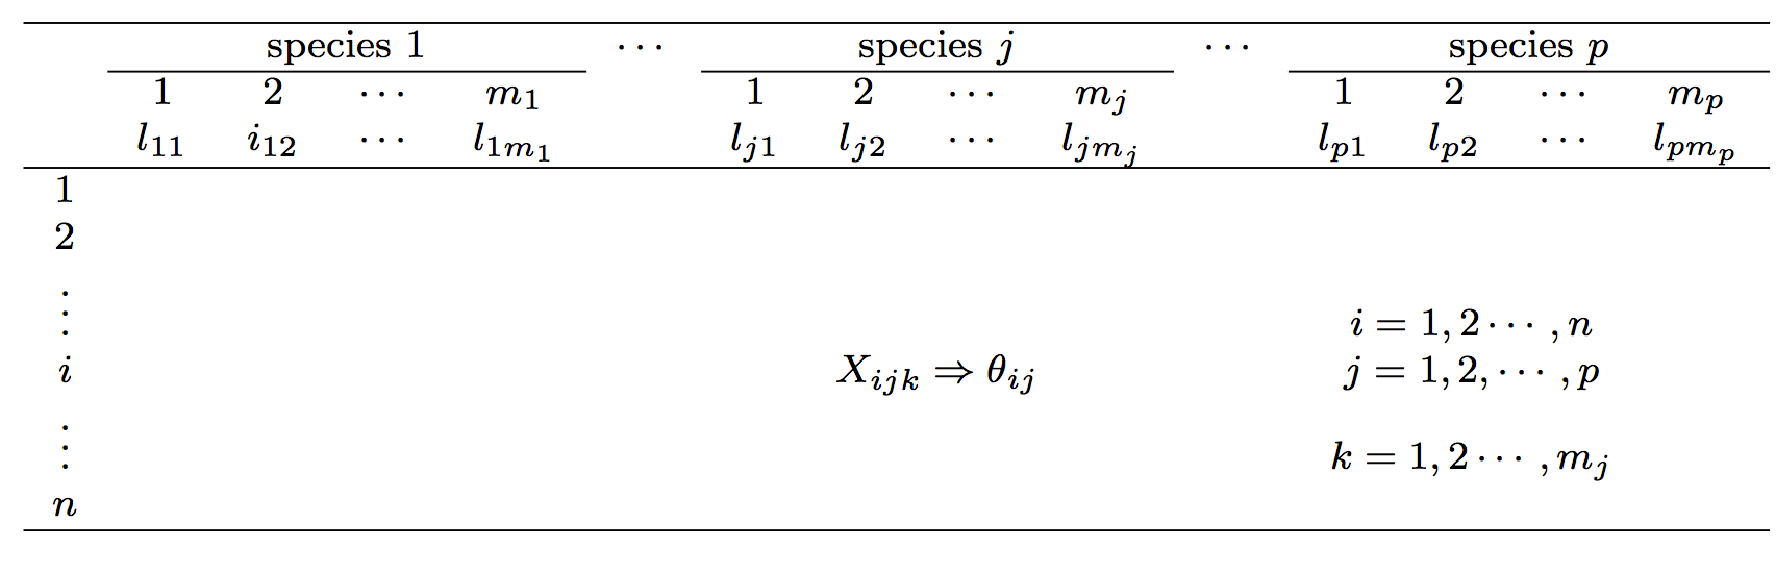
\includegraphics[scale=0.5,trim=0 0 0 0,clip]{Figure/F32_table.pdf}}
\caption[Summary of read count data that aligned to clade-specific markers]{Summary of read count data that aligned to clade-specific markers. The sequencing reads from $n$ metagenomic samples are aligned to a set of $m_j$ clade-specific marker genes for the $i$th species  for a total of $p$ species, where $X_{ijk}$ is  the number of reads that are assigned to the $k$th marker gene of the $j$th species for the $i$th sample.  $\theta_{ij}$ is the relative abundance of $j$th species in the $i$th sample and this is the parameter we want to estimate.}
\label{F32_table}
\end{figure*}


\begin{figure*}[htb]
	\centering
	%\adjustbox{trim={.15\width} {.06\height} {0.1\width} {.06\height},clip}%
	{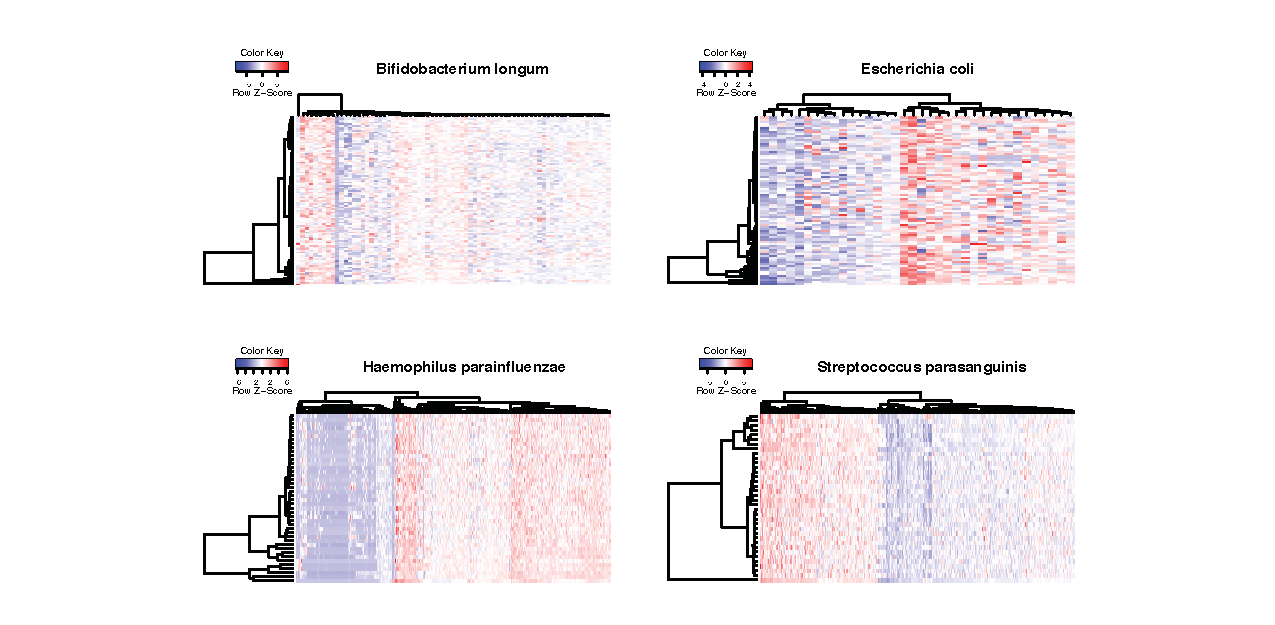
\includegraphics[scale=0.95,trim=80 0 0 0,clip]{Figure/F31_Marker_Effects.pdf}}
	\caption[Marker effects in the shotgun metagenomic data for four bacterial species]{Marker effects in the shotgun metagenomic data for four bacterial species. The raw sequencing reads were first aligned to the taxonomic markers and then normalized as the number of aligned read for each marker divided by marker length and total number of aligned reads for each sample. The normalized data was then clustered and showed in heatmap. The rows are  samples and columns are taxonomic markers from {\it MetaPhlAn}. }
	\label{F31_Marker_Effects}
\end{figure*}



\subsection{A multi-aample Poisson model to account for marker-specific effects}


Consider a metagenomic study with $N$ samples. After the sequencing reads are aligned to sets of clade-specific marker genes, the data can be summarized as a large table of counts as shown in Figure~\ref{F32_table}, where $X_{ijk}$ is  the count data of sequencing reads  for sample $i~(i = 1,2,\ldots,n)$, species $j~(j = 1,2,\ldots,p)$ and marker $k~(k = 1,2,\ldots,m_j)$. 
We model the count data for all species and all samples together and assume that the count  $X_{ijk}$ is generated from the following Poisson model,
\begin{equation*}
X_{ijk} \sim \mbox{Poisson}(\theta_{ij}t_{i}\phi_{jk}l_{jk}),
\end{equation*}
where $\theta_{ij} > 0$ is the relative abundance for the $j$th species in the $i$th sample. In common practice, the bacterial abundance are usually transformed into relative abundances (i.e. the bacterial abundance sum to 100\% in one sample).  We therefore impose that  $\sum_{j=1}^{p} \theta_{ij} = 1$. This constraint also avoids the identifiability issue in the model.  Here $t_i$ is the total read counts for sample $i$ that are mapped to the marker genes and $l_{jk}$ is the  length of the $k$th marker gene for $j$th species. Note that the species may have different number of markers. $t_i$ and $l_{jk}$ are known or can be calculated from the data directly.  The parameters $\phi_{jk} >0 ~(j=1, \cdots, p \textrm{ and } k=1,\cdots, m_j)$ are used to model  the market-specific effects for the set of  marker genes. The marker-specific effect can  be due to different GC contents, mappability and possible lateral gene transfers.  Our model uses data from multiple samples to estimate the marker effects $\phi_{jk}$.  When $\phi_{jk}=1$, our model is a Poisson model without considering the marker effects, which is essentially the approach used by {\it MetaPhlAn}.


\subsection{Model fitting}
We fit the model  and estimate the parameter using the maximum likelihood estimation, where the   likelihood   function is
\begin{align*}
L & = \prod_i\prod_j\prod_k \frac{e^{-\theta_{ij}t_{i}\phi_{jk}l_{jk}}(\theta_{ij}t_{i}\phi_{jk}l_{jk})^{x_{ijk}}}{x_{ijk}!},
\end{align*}
and its logarithm is 
\begin{align*}
\log L =  &  
\sum_i\sum_j\sum_k (-\theta_{ij}t_{i}\phi_{jk}l_{jk}+x_{ijk}log(\theta_{ij}t_{i}\phi_{jk}l_{jk})-log(x_{ijk}!)).
\end{align*}
Estimates $\theta$ and $\phi$ can be obtained iteratively.  We  first estimate all $\theta_{ij}$ by fixing  $\phi_{ik}$ at the current values, 
\begin{align*}
\hat \theta_{ij} = \frac{\sum_kx_{ijk}}{t_{i}\sum_k\phi_{jk}l_{jk}}, 
\end{align*}
and then normalize these values so that $\sum_{j=1}^p\hat{\theta}_{ij}=1$ for $i=1,\cdots, n$.
We estimate all $\phi_{ik}$ by fixing  $\theta_{ij}$ at the current values, 
\begin{align*}
\hat \phi_{ik} = \frac{\sum_ix_{ijk}}{l_{jk}\sum_i\theta_{ij}t_{i}}.
\end{align*}

We iteratively update  $\theta_{ij}$ and $\phi_{ik}$ until convergence. Since the closed-form updating formula are available, the algorithm is very efficient. 




\section{Simulation studies}
%\subsection{Simulation based on the multi-sample Poisson model}
We  first performed  a simulation study to examine the model fitting, where we simulated different sample size $n=(20,50,100)$ and different number of markers $m=(20,50,100)$ per species. In order to mimic the skewed distribution of species abundance in a sample, we simulated $\theta_{ij}$ from a log-normal distribution with $\mu=0$ and $sd=1.5$. The simulated $\theta_{ij}$ were then normalized so that    $\sum_{j=1}^{p} \theta_{ij} = 1$. The scaled marker length $l_{jk}$ and total read counts $t_i$ was simulated uniformly from [0.1,10] and [50,500], respectively. We simulated $\phi_{jk}$ from a log-normal distribution with $\mu=0$ and $sd= 1.5$. We fitted the MSSQ model on the simulated data and  then calculate the average relative difference (AVGRD) for  $\hat\theta$ and $\hat\phi$, which is defined as
$$\frac{1}{n}\sum_i^n \frac{|\theta_{ij}-\hat{\theta}_{ij}|}{\hat{\theta}_{ij}}, \mbox{  }
\frac{1}{m}\sum_k^m \frac{|\phi_{jk}-\hat{\phi}_{jk}|}{\hat{\phi}_{jk}}.
$$ 
The simulations were repeated 1,000 times for each combination of sample size and marker size. The mean and standard error of the AVGRD over 1000 repeated simulations were then calculated and reported.

Table~\ref{MSSQTable1} shows the simulation results. When the number of markers per species is fixed, increasing  sample size improves the estimation accuracy of both $\theta$ and $\phi$. Similarly, when the sample size is fixed, more markers can improve the estimation accuracy of both $\theta$ and $\phi$.

\begin{table}[ht]
	\caption[Parameter estimation for data simulated from the multi-sample Poisson model]{Parameter estimation for data simulated from the multi-sample Poisson model with different sample size $n$ and different marker size $m$.  For each parameter, the mean and standard error (SE) of average relative difference (AVGRD) are calculated based on 1000 replications. For each $n$ and $m$, the first row are estimates for $\theta$; the second row are for $\phi$.   
		\label{MSSQTable1}}
	\begin{center}	\begin{tabular}{lrrrrrrrrrr}
			\hline
			AVGRD& & \multicolumn{2}{c}{$m = 20$} & \multicolumn{2}{c}{$m = 50$}  & \multicolumn{2}{c}{$m = 100$}    \\
			\cline{3-8}
			& & mean & SE & mean & SE & mean &  SE &  \\
			%%%%
			%%%%
			\hline
			%%%%
			$n$=20 & $\theta$ & 0.19 & 0.05 & 0.14 & 0.04 & 0.11 & 0.03  \\
			& $\phi$ & 0.22 & 0.07 & 0.16 & 0.05 & 0.13 & 0.03  \\
			$n$=50 & $\theta$ & 0.09 & 0.02 & 0.07 & 0.01 & 0.06 & 0.01  \\
			& $\phi$ & 0.08 & 0.02 & 0.07 & 0.02 & 0.07 & 0.01  \\
			$n$=100 & $\theta$ & 0.06 & 0.01 & 0.05 & 0.01 & 0.04 & 0.01  \\
			& $\phi$ & 0.04 & 0.01 & 0.04 & 0.01 & 0.04 & 0.01  \\
			
			%%%%%
			%%%%%
			\hline
		\end{tabular}
	\end{center}
\end{table}


We next  studied the effects of allowing the marker-specific effects in the Poisson on species abundance quantification, where we simulated $n=50$ samples and each sample had $p=50$ species.  The true abundance $\theta_{ij}$, the scaled marker length $l_{jk}$ and total read counts $t_i$ were simulated in the  same way  as previously. For each species, the number of markers $m_j$ was uniformly simulated from [10,50]. To mimic  different degrees of marker effects, we simulated $\phi_{jk}$ from a log-normal distribution with $\mu=0$ and $sd=(0, 0.5, 1, 1.5)$ for four different simulation settings, respectively. The simulation setting with log-normal($\mu=0$, $sd=0$) indicates no marker effect in the data and the other three settings indicate increasing marker effects.


We observed that ignoring the marker-specific effects led to large biases in  the estimates of the abundance $\theta_{ij}$, as shown in Figure \ref{F33_2016_02_07_Abundance_Estimation_Scale5_100_Merge} (full-scale in upper panel and zoomed-in to 0-5\% scale in lower panel). When the marker effect increases, the estimated abundance deviated more from the true abundance, where the mean of AVGRD were  0.07, 0.15, 0.28, 0.52.  In contrast, estimates of the relative abundances from MSSQ showed  little biases when there were strong maker-specific effects. The mean of AVGRD were 0.07, 0.09, 0.09, 0.10, respectively. 

\begin{figure*}[ht]
	\centering
	%\adjustbox{trim={.0\width} {.15\height} {.0\width} {.0\height},clip}%
	{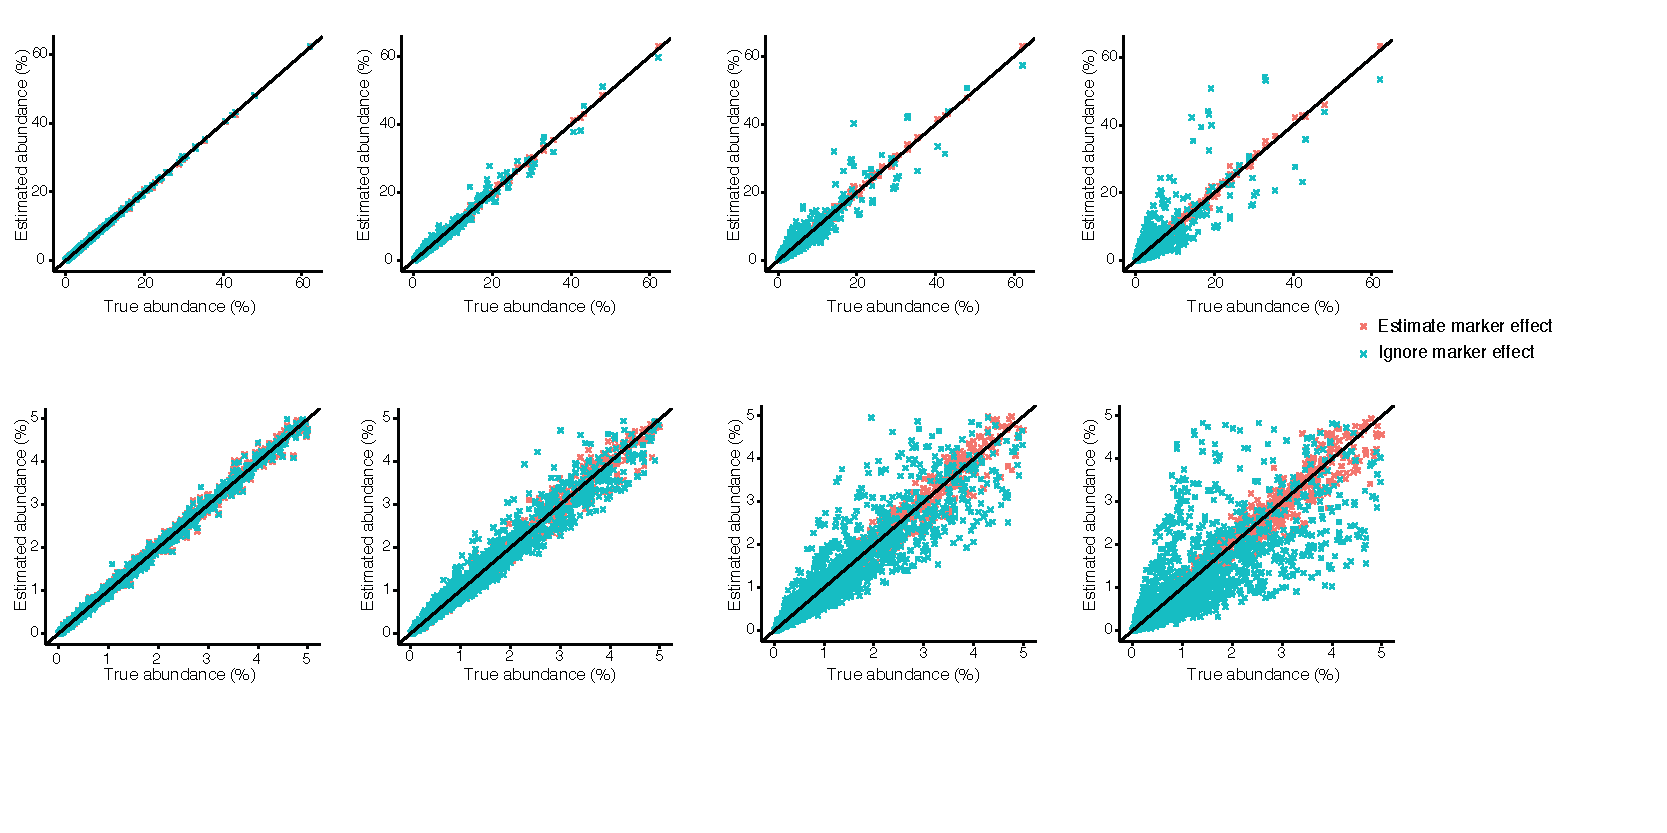
\includegraphics[scale=0.53,trim=0 60 20 0,clip]{Figure/F33_2016_02_07_Abundance_Estimation_Scale5_100_Merge.pdf}}
	\caption[Comparison of relative abundance estimation by MSSQ  with and without estimating marker effect]{Comparison of relative abundance estimation by MSSQ  with and without estimating marker effect ($\phi_{jk}=1$) for four scenarios with increasing marker-specific effects (from left to right). A total of 50 samples, each with 50 species were simulated. Upper panel, full scale; lower panel, zoom-in 0-5\% scale  }
	\label{F33_2016_02_07_Abundance_Estimation_Scale5_100_Merge}
\end{figure*}



\section{Application to the human gut microbiome data}
\label{sec:realdata}
\subsection{Data description and processing} 
We applied MSSQ to a data set of shotgun metagenomic study comparing gut microbiome between healthy children and children with Crohn's disease \citep{lewis2015inflammation,lee2015comparative}. A total of 90 children with  Crohn's disease  and 26 healthy controls were recruited to the study and  provided fecal samples for  shotgun metagenomic sequencing.  DNAs were prepared from whole stool and were sequenced using the Illumina HiSeq paired-end method, resulting in an average number of reads per sample of $11 \times 10^6$ with an average length 100 bases on each end of the paired-end read. We were  interested in quantifying the bacterial abundances and identifying the  bacteria species that show differential abundance between the normal samples and the Crohn's disease samples.


We first aligned the sequencing reads  to the {\it MetaPhlAn} clade specific markers for each of the bacterial species.  In order to compare our method with {\it MetaPhlAn}, we applied the same filtering criteria used by {\it MetaPhlAn}. Specifically,  for each species, we filtered out the upper 10\% percentile of the most abundant markers and lower 10\% percentile least abundant markers. We replaced the read counts of those filtered markers with NAs and our model ignores the NAs in the model fitting procedure. We ran  {\it MetaPhlAn} on the same data set and compare the results with those from MSSQ.


\subsection{Abundance estimation with MSSQ}
After the filtering steps, we applied MSSQ to  quantify the  species abundance from healthy children and those with Crohn's disease separately. MSSQ identified a total of 138 species presented in the control samples and 216 in the disease samples.  {\it MetaPhlAn} identified the same number of species in control and disease samples. 


We then compared the abundance estimation by MSSQ and {\it MetaPhlAn} (Figure~\ref{PLEASE_COMBO_Abundance_Estimation}). When  the marker-specific  effects were excluded from the model, i.e., setting all $\phi_{jk}$=1, as expected, MSSQ resulted in  the same abundance estimate as the {\it MetaPhlAn} for both control and disease samples. When the marker-specific  effects were estimated, MSSQ shows different abundance estimation from  {\it MetaPhlAn}. Overall, we observed that the estimates from both methods were comparable with a Pearson correlation of 0.92 (See Figure \ref{PLEASE_COMBO_Abundance_Estimation} upper panel). However, for low abundant species, a large discrepancies of the estimates were observed (Figure \ref{PLEASE_COMBO_Abundance_Estimation} lower panel).  Due to low read counts to these species, a large variability in these estimates were expected. The overall pattern was similar to our simulation results in Figure \ref{F33_2016_02_07_Abundance_Estimation_Scale5_100_Merge}. We also observed that the differences were greater in disease samples than in the control samples.

\begin{figure}[ht]
\centering
{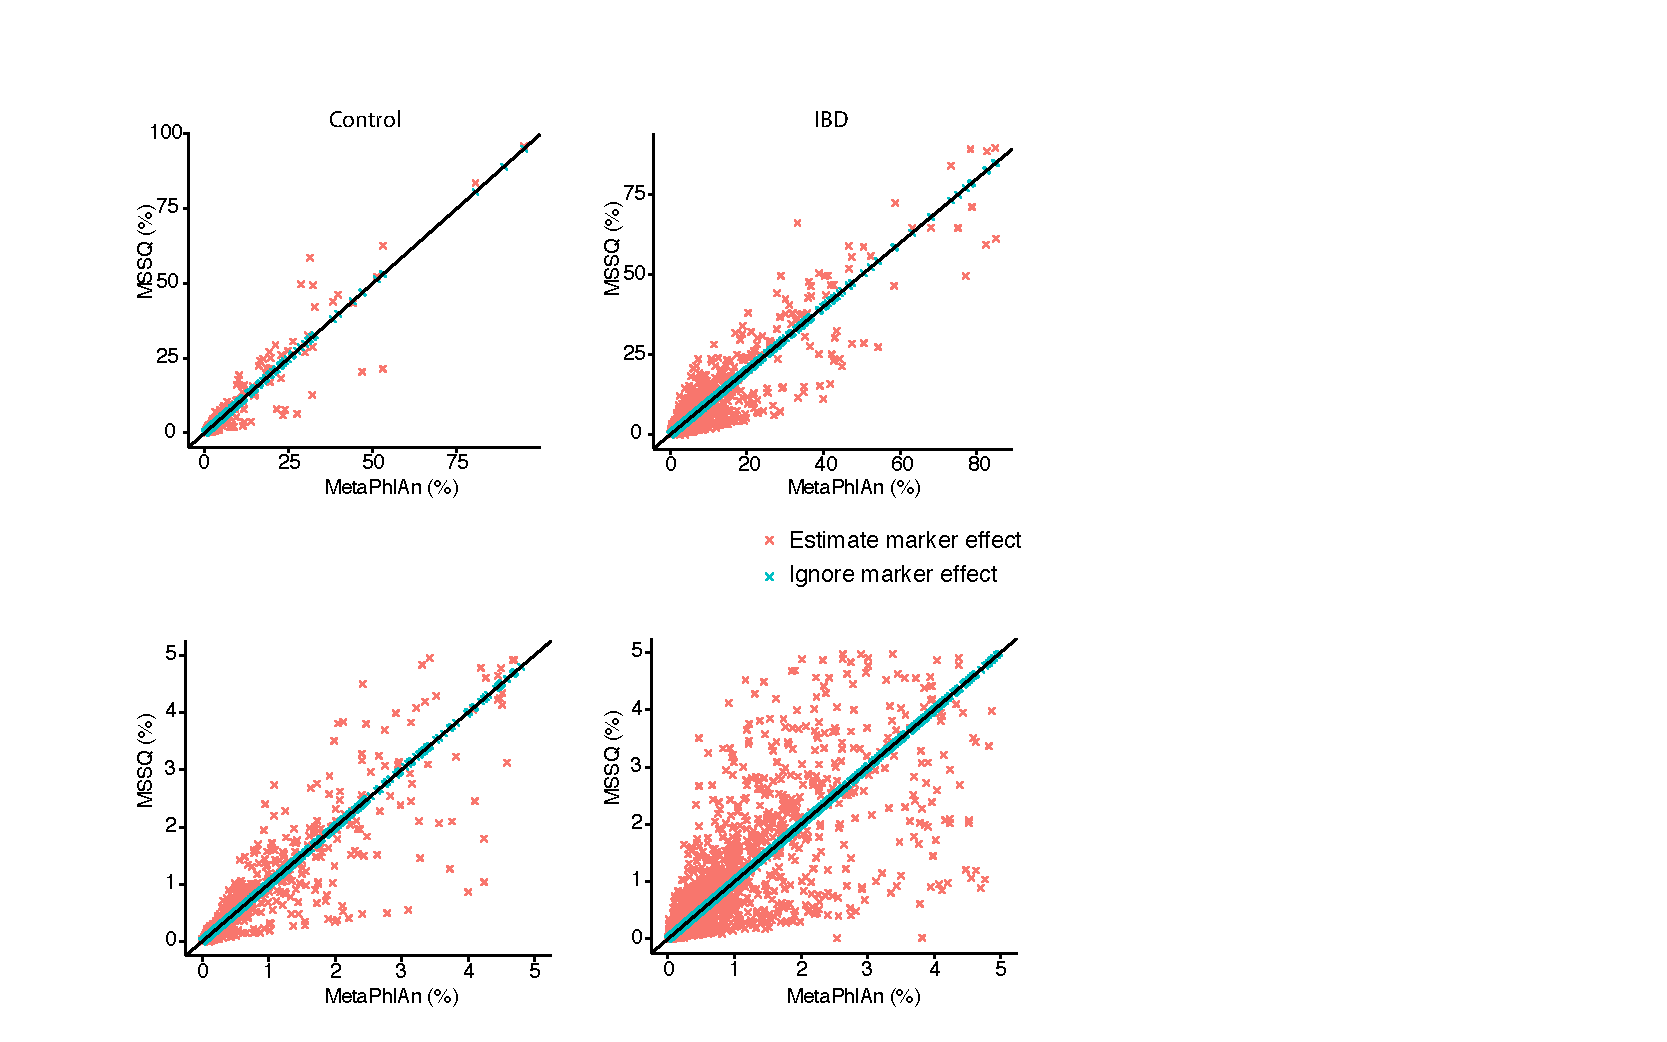
\includegraphics[scale=0.8,trim=20 10 150 0,clip]
{Figure/F34_2016_02_01_PLEASE_COMBO_Abundance_Estimation_Merge.pdf}
}
\caption[Comparison of estimated relative abundances from MSSQ and {\it MetaPhlAn}]{Comparison of estimated relative abundances from MSSQ and {\it MetaPhlAn}. Upper panel: all species; Lower panel: species with abundances $<5\%$. }
\label{PLEASE_COMBO_Abundance_Estimation}
\end{figure}


\subsection{Clustering and differential abundance analysis}
We next evaluated whether the abundance quantification by MSSQ can improve the downstream analysis such as clustering and differential abundance analysis. Before we performed the downstream analysis, we first filtered out the rare species, which is a common pre-processing procedure  often used in the literature \citep{Kostic:2015bh,Romero:2014il,Stein:2013dl}. Particularly, the species with an estimated abundance $< 1\%$ in all the control and disease samples in both MSSQ and {\it MetaPhlAn} estimation were filtered out. After filtering, 136 species were left for following analysis. 

Figure \ref{F35_2016_02_01_Heatmap_Merge} shows the heatmap of the estimated abundances from MSSQ and {\it MetaPhlAn}, where the samples were clustered with  Bray-Curtis distance and the species were clustered based on Pearson's correlations. We observed a clear separation of normal and Crohn's disease gut microbiome samples based on {\it MetaPhlAn} and MSSQ estimation of the species abundances.  However, the clustering results based on the MSSQ estimation show a clearer pattern. 




\begin{figure*}[th]
	\centering
	{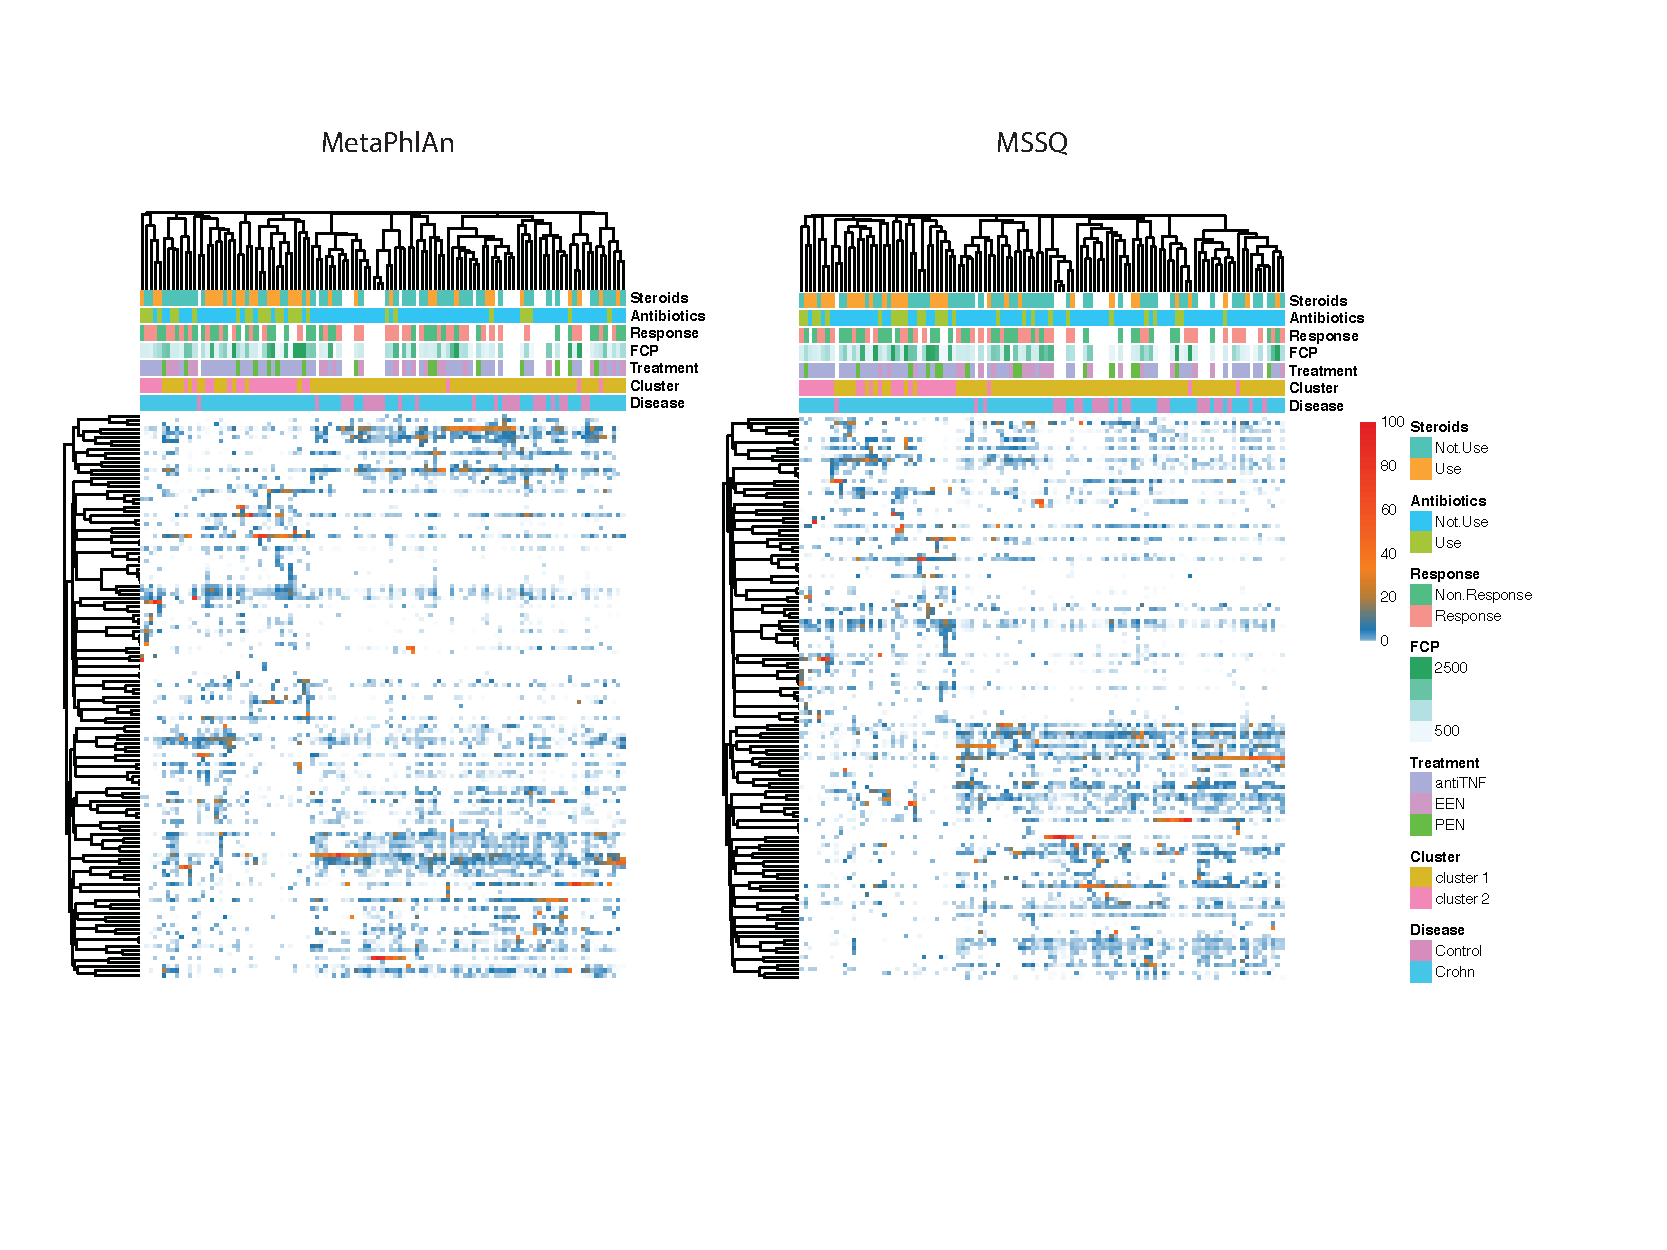
\includegraphics[scale=0.6,trim=30 140 0 0,clip]{Figure/F35_2016_02_01_Heatmap_Merge.pdf}
	}
	\caption[Heatmap of the estimated abundances from MSSQ and {\it MetaPhlAn}]{Heatmap of the estimated abundances from MSSQ and {\it MetaPhlAn} based on analysis of metagenomic data comparing normal samples and those with Crohn's disease.  Clinical meta-data are presented in the top bars. See \cite{lewis2015inflammation} and \cite{lee2015comparative} for details of the clinical meta-data. }
	\label{F35_2016_02_01_Heatmap_Merge}
\end{figure*}


As a comparison, we also tested for differential abundance between control and disease samples for each species using the Wilcoxon rank-sum test. Using these estimated abundance from {\it MetaPhlAn}, Wilcoxon rank-sum test identified 39 differentially abundant species with  FDR adjusted $p$-value $<$ 0.05. Based on the estimated abundance from MSSQ, 41 species were identified to be differentially abundant between control and disease samples, including all 39 differentially abundant species identified based on the {\it MetaPhlAn} estimation. Among the species that are more abundant in Crohn's patients, {\it E. coli, Bacteroides, Enterococcus, Klebsiella}, and {\it  Ruminococcus gnavus} have been reported in literature \citep{Sartor, Liu95}. Among the protective species, {\it Bifidobacterium, Roseburia} and {\it Eubacterium} were also reported in previous studies \citep{manichanh2012gut}. \cite{manichanh2012gut} detected {\it Lactobacillus} as a protective species that was more abundant in normal gut. 

The two species that were only identified when MSSQ was applied include  {\it Coprococcus comes}, which belongs to genera {\it Coprococcus}, and {\it Clostridium symbiosum}. Both  species were reported to be associated with dysbiosis, CD \citep{gevers2014treatment} and UC \citep{du2015development}.  {\it Clostridium symbiosum} has been reported to protect the gut mucosa by producing butyrate \citep{van2013butyrate}.


\subsection{Comparing marker effect in control and disease samples}
Figure~\ref{F33_Marker_Effect_Boxplot} shows the estimated marker effect $\hat{\phi}$ for each species in normal control and disease samples. The dispersion of $\hat{\phi}$ values indicates the marker effects indeed present in the real data. The average dispersion of $\hat{\phi}$ is 43.10 for species in control samples and 729.12 for species in disease samples, where the dispersion was measured by the standard deviation. 

\citet{Korem:2015cv} studied the bacterial growth dynamics using shotgun metagenomic data. They observed that when the bacteria is in replication status, the read coverage is not uniformly distributed across the bacterial genome. They further showed that bacterial growth dynamics are associated with diseases such as diabetes and Crohn's disease. Specifically, they found that the growth dynamics of two bacterial species Bifidobacterium longum and Escherichia coli are associated with Crohn's disease. We are interested to see if our model can capture the bacterial growth dynamics. We examined the estimated marker effects ($\phi$) for those two species between control and Crohn's disease samples in our metagenomic study (Figure~\ref{F36_Science_Five_Species}). We also plotted the estimated marker effects from several non-association species in \citet{Korem:2015cv} as negative control. Interestingly, the marker effects estimated from MSSQ show great difference between control and disease groups. No significant difference is observed for the other negative controls. This result indicate that marker effects ($\phi$) from MSSQ capture the bacterial growth dynamics and the difference in growth rate is associated with disease status. The bacterial relative abundance and growth dynamics are not necessarily correlated. MSSQ captures these two biological features.

\begin{figure*}[p]
	\centering
	{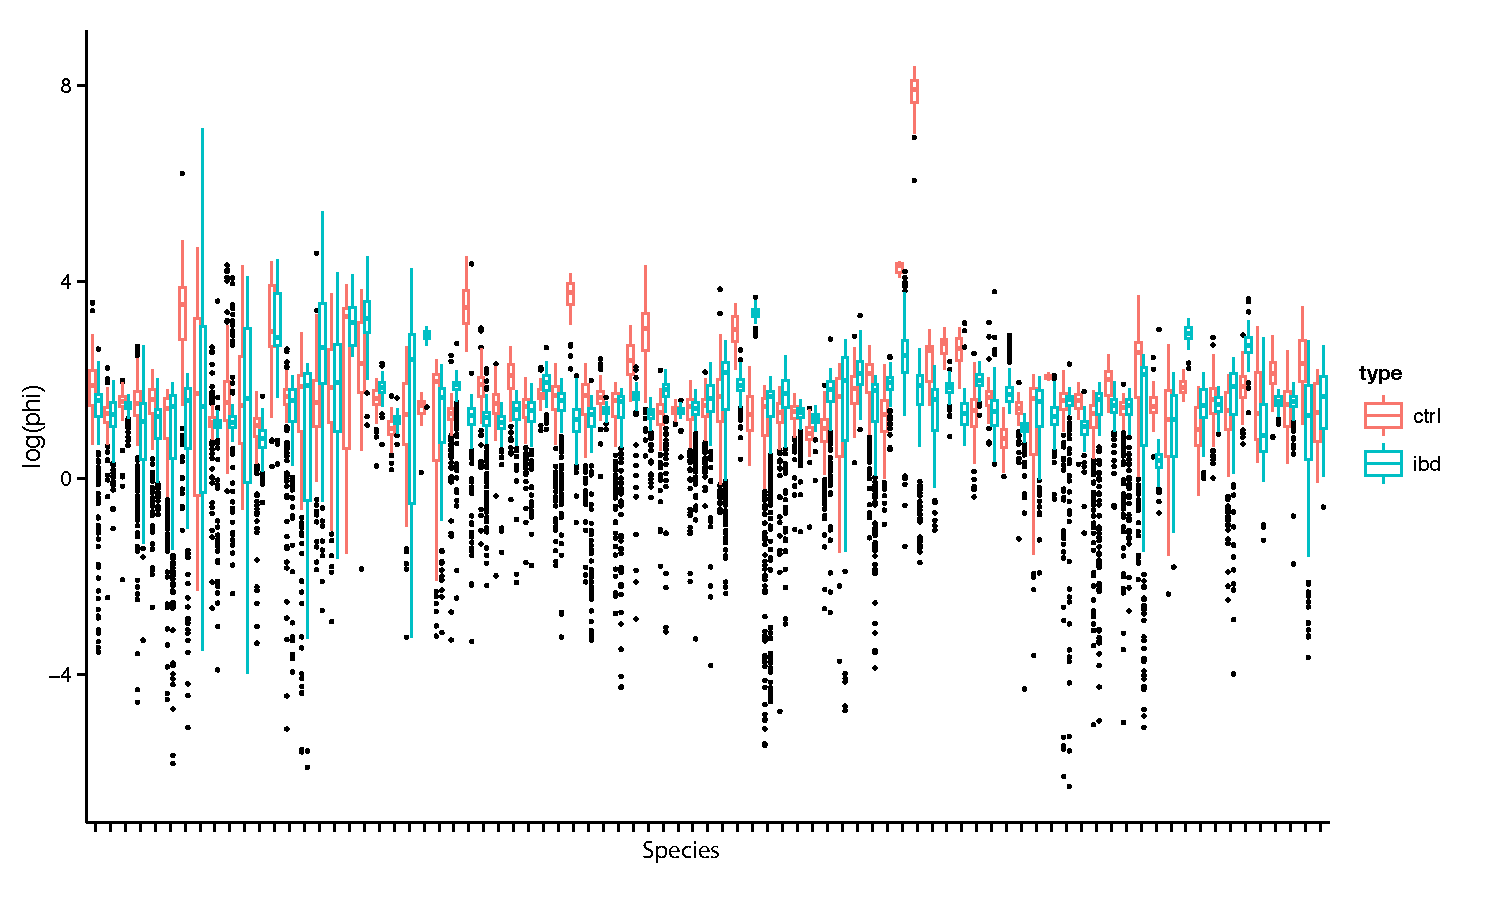
\includegraphics[scale=0.6,trim=0 20 0 0,clip]{Figure/F33_Marker_Effect_Boxplot.pdf}
	}
	\caption[Distribution of estimated marker-specific effects]{Distribution of estimated marker-specific effects for each species in the control samples  (upper panel) and disease samples (lower panel). Each dot represents the estimated $\phi$ with log transformation and each boxplot represents a species.}
	\label{F33_Marker_Effect_Boxplot}
\end{figure*}


\begin{figure*}[p]
	\centering
	%\adjustbox{trim={.0\width} {.0\height} {0.0\width} {.0\height},clip}%
	{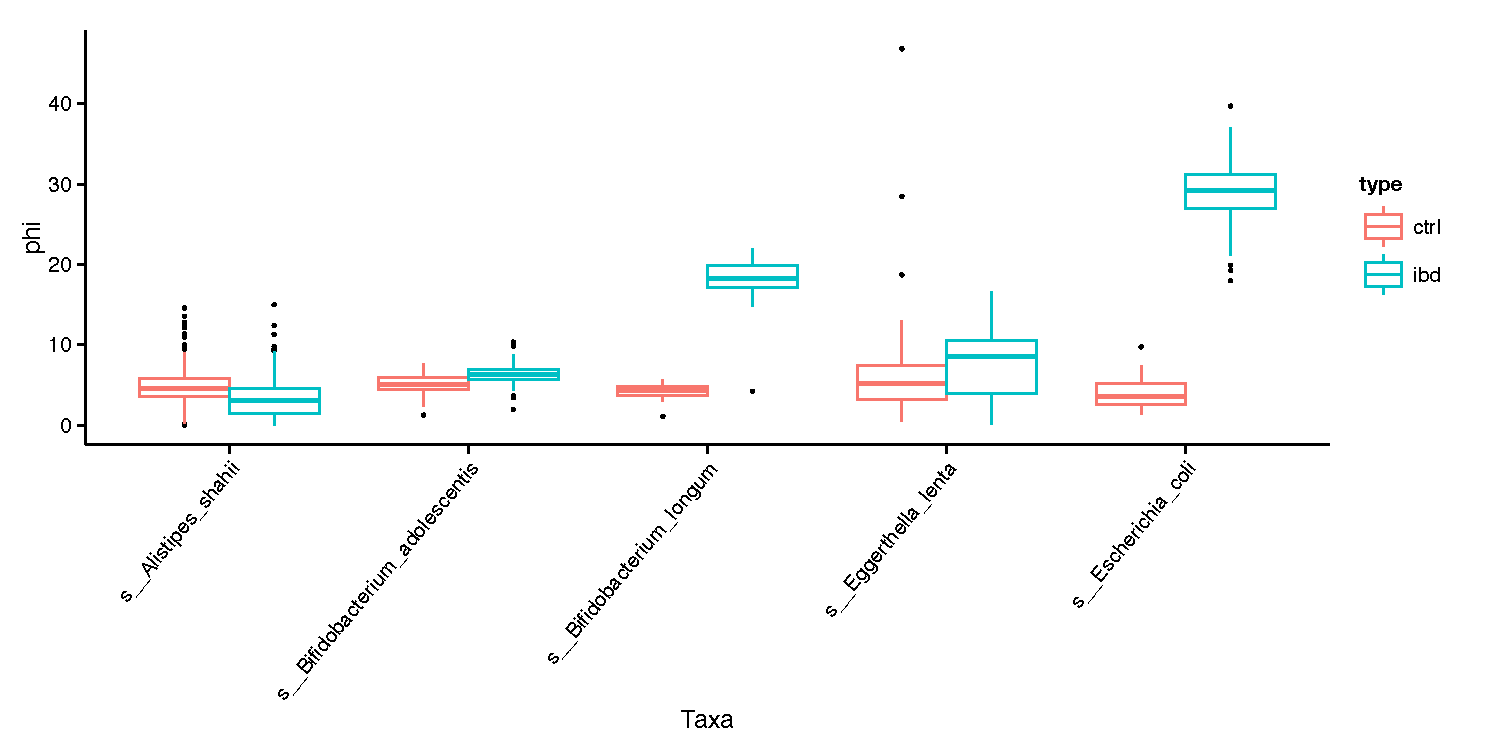
\includegraphics[scale=0.55]{Figure/F36_Science_Five_Species.pdf}
	}
	\caption[MSSQ captures the bacterial growth dynamics]{MSSQ capture the bacterial growth dynamics. \citet{Korem:2015cv} showed the growth dynamics of two bacterial species Bifidobacterium longum and Escherichia coli are associated with Crohn's disease. The estimated marker effects ($\phi$) for those two species between control and Crohn's disease samples in our metagenomic study are plotted. Three non-association species in \citet{Korem:2015cv} are also plotted as negative control.}
	\label{F36_Science_Five_Species}
\end{figure*}




\section{Discussion}
We have proposed a multi-sample Poisson model to quantify the bacterial abundances based on the shotgun metagenomic data.  Our method uses the count data of reads  aligned to clad-specific  marker genes  to quantify  the species abundances,  taking into account the marker effects that are observed in the shotgun sequencing data. In our analysis of real data, we used the marker genes sets used in  {\it MetaPhlAn} package.  Alternatively, one can also use the 40 universal marker genes defined by \cite{Sunagawa:2013if}. It would be interesting to compare whether different marker genes lead to similar species quantification. 
Simulation results indicate that the proposed model-based approach can lead to better quantification of species abundances.

We further demonstrated the proposed methods in an analysis of pediatric gut microbiome to identify the species that are associated with Crohn's disease. The discrepancy of the differential abundant species identified by MSSQ and {\it MetaPhlAn} is due to whether the maker-specific effects are accounted in the estimation. Our simulations have clearly demonstrated the ignoring such marker-specific effects can lead to biased quantification of the species abundances. The marker-specific effects could originates  from different sources. For example, it is well known that the sequencing reads are not uniformly distributed among genomic regions and are correlated with GC contents of the genomic regions \citep{ross2013characterizing}. Further, the copy number variation of the genes can also contribute to the under- or over- presentation of certain gene regions. Sequencing error and alignment error are other potential sources for non-uniform distribution of the reads and may cause the large  marker-to-marker variability we observed in the data. 

In our analysis, we fitted the multi-sample Poisson model for all the species and all the samples simultaneously. Since we do not expect to observe all the species in all the samples,  some regularization on the relative abundance parameter $\theta_{ij}$ may help to improve  the abundance quantification. Finally, it is interesting to establish the asymptotic distribution of the resulting estimates of the relative abundances when both the sample size $n$ and the numbers of marker genes $m_j$ go to infinity. 


%% --------------- ZIBR -------------------%%
\chpt{A two-part mixed-effect model for analyzing longitudinal microbiome compositional data} \label{chpt4:ZIBR}


In this chapter, a statistical model is proposed for longitudinal microbiome data analysis. Longitudinal measurements of microbial communities are commonly obtained in many microbiome studies. A key question in such microbiome studies is to identify the microbes that are associated with clinical outcomes or environmental factors. However, the longitudinal microbiome compositional data are highly skewed, bounded in [0,1), and often sparse with many zeros. In addition, the observations from repeated measures are correlated. A method that takes into account these features is needed for association analysis in longitudinal microbiome data. In this chapter, we propose a two-part zero-inflated Beta regression model with random effects (ZIBR) for testing the association between microbial abundance and clinical covariates for longitudinal microbiome data. The model includes a logistic regression component to model presence/absence of a microbe in samples and a Beta regression component to model non-zero microbial abundance, where each component includes a random effect to take into account the correlations among repeated measurements on the same subject. Both simulation studies and the application to real microbiome data show that ZIBR model outperforms the previously used method. This provides a useful tool for identifying the relevant taxa based on longitudinal or repeated measures in microbiome research.
The model was implemented in R package ZIBR and freely available at https://github.com/chvlyl/ZIBR.



\section{Introduction}
The human microbial communities are associated with many human diseases such as obesity, diabetes and inflammatory bowel disease (IBD) \citep{turnbaugh2006obesity, qin2012metagenome, Kostic:2015bh}. In order to decipher the function and impact of the microbes on the human well-being, two high-throughput sequencing based approaches have been widely used in microbiome studies. One is the 16S ribosomal RNA (rRNA) sequencing approach, which profiles bacterial community by sequencing the 16S rRNA marker gene. Another approach is the shotgun sequencing, which sequences all the microbial genomes presented in the sample, rather than just one marker gene. Both 16S rRNA and shotgun sequencing approaches are quite useful and have been widely applied to human microbiome studies, such as the Human Microbiome Project (HMP) \citep{turnbaugh2007human} and the Metagenomics of the Human Intestinal Tract (MetaHIT) project \citep{qin2010human}. To quantify the microbial abundance, the sequencing reads usually are aligned to some known reference sequences \citep{segata2012metagenomic}. Due to the uneven total sequence counts of samples, the microbial abundance measured in read counts are not comparable across samples. Therefore, it is common that the read counts are normalized to the relative abundance by dividing total sequence counts in the sample so that the relative abundances of all microbes in one sample sum to one \citep{tyler2014analyzing}, resulting in compositional data with lots of zeros. 


It is of great interest to study how microbial abundance changes across time and its association with treatments, clinical outcomes or other covariates. To address this question, many microbiome studies employed the longitudinal study design (for reviews, see \cite{Faust:2015bd, Gonzalez:2012gv, Gerber:2014ca}). For example, \citet{lewis2015inflammation} studied the gut microbiome from pediatric IBD patients during an eight-week treatment. One interesting question in this study is to identify the bacterial taxa that change their abundance under different treatments across time. In another longitudinal microbiome study, \citet{Backhed:2015kc} studied the microbiome change during the first years of newborn babies with different delivery methods and feeding activities. 


Modeling such sparse longitudinal compositional data is challenging for several reasons. First, the microbiome compositional data is non-normally distributed and bounded in [0,1). Methods with normal distributional assumption are not expected to perform well. Second, the microbiome data is often observed with many zeros, which leads to great heterogeneity in the data. Third, in microbiome studies, it is important to adjust for the other covariates/confounders such as patient age or antibiotics use. Therefore, a multivariate regression based method is more preferred than univariate tests such as the t-test or Wilcoxon rank test. Fourth, the repeated measurements in the longitudinal data are correlated, i.e, observations from the same subject across time are not independent. This renders the methods with independence assumption not directly applicable. Ignoring the correlation among repeated measures can lead to incorrect inference. Therefore, taking into account the correlation among repeated measurements is necessary. 


Several methods have been used to analyze the longitudinal data in order to identify the covariate-associated taxa, but with their own limitations. To overcome the issue of non-independence of the data across time points, most of the longitudinal microbiome studies analyzed data at individual time point \citep{Cox:2014hy, arrieta2015early, Rutten:2015bx, Zhou:2015kw, David:2014cl, Schulz:2014fy} or compared two time points but ignored the other time points \citep{Backhed:2015kc, Koren:2012ji}. To take into account the excessive zeros in the data, a two-part test combining a Z-test for testing the proportion of zeros and a Wilcoxon rank-sum test for testing the non-zero values, was developed for identifying differential abundant microbes between two groups \citep{wagner2011application, markle2013sex}. Such tests cannot be applied to longitudinal correlated data and are limited to only two-group comparison. \citet{Romero:2014il} used a zero-inflated Poisson regression model with random effect to take into account the correlations in longitudinal data, but the model can only be applied to count data. A linear mixed effect model with arcsine square root transformation on the microbiome compositional data was used \citep{LaRosa:2014kk, Kostic:2015bh}, however, this method does not explicitly handle the excessive zeros in the data. This motivates us to develop a flexible method that identifies the covariate-associated taxa while handling the features of the microbiome compositional data and jointly modeling data from all time points. 


The focus of this chapter is to develop a statistical model for identifying the bacterial taxa that are associated with covariates while addressing the above limitations. We propose a two-part mixed-effect zero-inflated Beta regression model, which is a mixture of a logistic regression component and a Beta regression component, with the random effects included in the model to allow the correlations between repeated measures. This model takes into account the nature of the microbiome compositional data and also allows for multiple covariates in the regression setting. In addition, the model can jointly analyze data from all the time points. Simulation results show that our method outperforms several previously used methods in terms of increased power in detecting covariate-associated taxa. We apply ZIBR to a real microbiome study and identify several bacterial taxa that are associated with different treatments of inflammatory bowed disease (IBD). ZIBR model was implemented in R package ZIBR and is freely available at https://github.com/chvlyl/ZIBR.


\section{A two-part mixed-effect regression model for longitudinal microbiome data}
To illustrate the features of the sparse compositional data observed  in microbiome studies, Figure \ref{Fig1} shows the distribution of the relative abundance of two bacterial genera from a real microbiome data set from \citet{lewis2015inflammation}.  The data show several important features: (1)  are  bounded in [0,1);  (2) the data highly skewed; (3) the data include  excessive zeros.   In addition, if the microbiome data are measured in a longitudinal study, the repeated measures from the same subjects across time points are expected to be correlated.  In order to identify the microbes that are associated with clinical outcomes, we develop a two-part logistic-Beta regression model with random effects to model such longitudinal data. 

\begin{figure}[!tpb]%figure1
\centerline{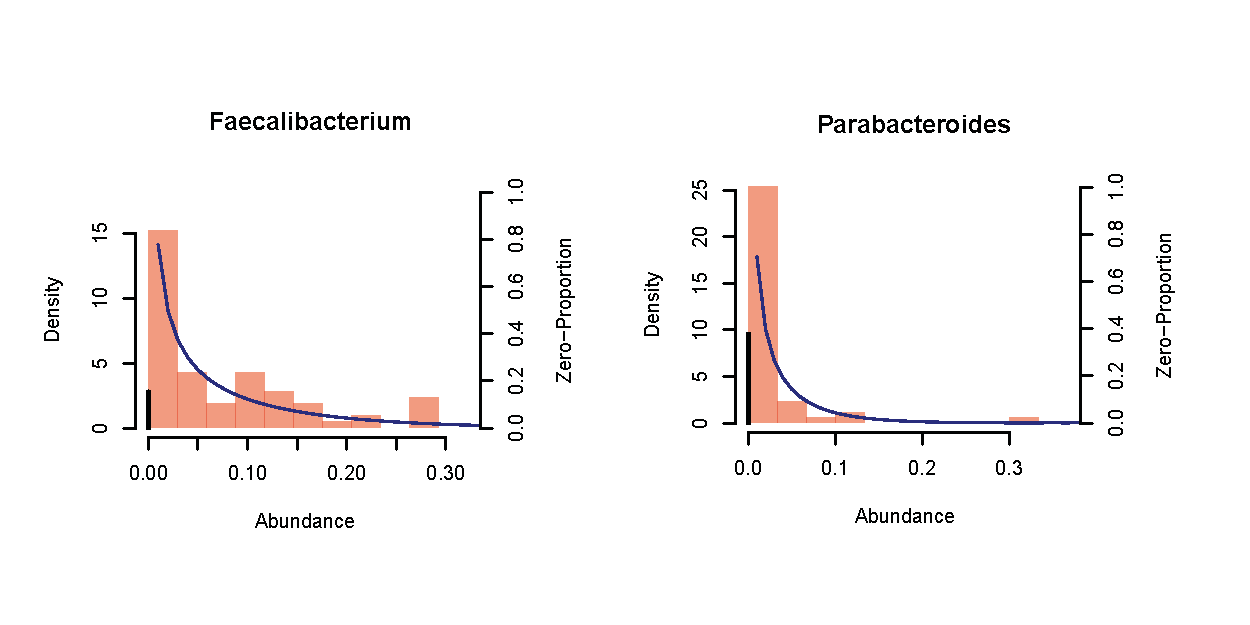
\includegraphics[scale=0.7,trim=0 40 0 0,clip]{Figure/F41_Distribution_of_Real_Data_v3.pdf}}
\caption[Examples of two genera from the real human microbiome data]{Examples of two genera from the real human microbiome data. Red bars represent the density of the non-zero data (left Y axis). Black bars represent the zero proportion (right Y axis). Back curves show  the fit of the non-zero data using a  Beta distribution.}
\label{Fig1}
\end{figure}

Our model considers each taxon separately. For each given bacterial taxon, let $Y_{it}~(i = 1,2,\ldots,N, t= 1,2,\dots,T)$ be its relative abundance for subject $i$ at time $t$, where $0 \le Y_{it} < 1$.   We assume that 
\begin{align}
Y_{it} &\backsim 0 \text{ with probability } 1-p_{it}\\
&\backsim \mbox{Beta}(\mu_{it}\phi,(1-\mu_{it})\phi) \text{ with probability } p_{it},
\end{align}
where the  density function of the Beta distribution is parameterized as
\begin{equation}\label{beta1}
f(y_{it};\mu_{it},\phi) = \frac{ \Gamma(\phi)}{ \Gamma(\mu_{it}\phi)\Gamma((1-\mu_{it})\phi)}y_{it}^{\mu_{it}\phi-1}(1-y_{it})^{(1-\mu_{it})\phi-1}
\end{equation}
with $\mu_{it}$ $(0<\mu_{it}<1)$ and $\phi$ $(\phi>0)$ being  the mean and dispersion parameters of the Beta distribution, respectively. The parameter $p_{it}$ is the probability that the observation $Y_{it}$ is generated from the Beta component. Figure \ref{Fig1}  shows that the Beta distribution fits  the non-zero values of the real data well.  In addition,  we let the probability $p_{it}$ of the logistic component and the mean of the Beta component $\mu_{it}$ depend on the covariates through the logit link function,
\begin{align}
\mbox{logit}(p_{it})&= \log\left(\frac{p_{it}}{1-p_{it}}\right) = X_{it}^T \alpha + a_i,\label{logit1}\\ 
\mbox{logit}(\mu_{it})&= \log \left(\frac{\mu_{it}}{1-\mu_{it}}\right) = Z_{it}^T \beta + b_i,\label{logit2}
\end{align}
where $a_i$ and $b_i$ are the individual-specific random intercepts,  $X_i$ and $Z_i$ are the covariates that can be time-dependent and are  not necessarily  the same, and $\alpha$ and $\beta$ are the corresponding vectors of the regression coefficients. 

This model can be considered as a two-part model with a logistic component and a Beta component. The logistic component  models the presence/absence of the taxon in the samples and the Beta component  models the non-zero abundance of the taxon.  A covariate can  affect the microbiome composition  in two different   ways: (1) it  affects the presence/absence of the taxon in the samples, which is modeled through the logistic regression part in the model; (2) it affects the relative abundance when the taxon presents in the samples. This is modeled by the Beta regression in the model. The data observed are from  a mixture of these two models.  This model is flexible to allow  that the covariates affecting  the presence/absence of the microbial species and the covariates affecting  microbial abundance to be different. 

If the data are measured at repeated times, the responses at different time points within a subject are expected to be correlated. The repeated measures $Y_{it}$ ($t=1,\ldots,T)$ on the same subject $i$ share the same individual-specific values of $a_i$ and $b_i$, which can be used to model such correlations.  We only include the random intercepts in the model since such  simple random intercepts are often adequate in practice \citep{min2005random} to capture the longitudinal correlations.  However, it is easy to extend our model to include   random slops. The random effects are assumed to follow an independent normal distribution, 
\begin{align*}
a_{i}  \sim N(0,\sigma_1^2), \quad 
b_{i} \sim N(0,\sigma_2^2).
\end{align*}


The parameters can be estimated by the standard maximum likelihood estimation (MLE), where  the likelihood function  is given as 
\begin{multline*}
L (\alpha,\beta, \phi, \sigma_1^2, \sigma_2^2)\\
= \prod_{i=1}^{N}\int_{-\infty}^{\infty}\int_{-\infty}^{\infty}  \prod_{t=1}^{T}(1- p_{it})^{I(Y_{it}=0)}[p_{it} f(\mu_{it},\phi)]^{I(Y_{it}>0)} \\
\times  g(a_i,b_i | \sigma_1^2,\sigma_2^2)\, \mathrm{d}a_i\mathrm{d}b_i,
\end{multline*}
where $p_{it}$ and $\mu_{it}$ are defined through the logistic regression models \eqref{logit1}-\eqref{logit2},  $f(\mu_{it},\phi)$ is the Beta density function given in \eqref{beta1} and $g(a_i,b_i | \sigma_1^2,\sigma_2^2)$  is  the product of two normal density functions. 

To evaluate this likelihood function, we first integrate out the unobserved random effects to obtain a marginal likelihood. Since the integrals are analytically intractable, the marginal likelihood does not have a closed-form. We use Gauss-Hermite quadrature to approximate the integral by a finite sum. The MLE of   $(\alpha, \beta, \phi, \sigma_1^2, \sigma_2^2)$ can be obtained numerically.
We use likelihood ratio test  for three  biologically interesting  null hypotheses:
\begin{enumerate}
\item  the covariates are associated  with the bacterial taxon  by affecting its presence or absence, 
$H_0: \alpha_j = 0$; 
\item the taxon  is associated with the covariates by showing different abundances, $H_0:\beta_j = 0$;
\item  the covariates affect the taxon   both in terms of presence/absence and its abundance, $H_0:\alpha_j=0~ and~ \beta_j=0$ for each covariate $X_j$ and $Z_j$.
\end{enumerate}
The $p$ values can be obtained for each of these hypotheses. If the covariate $X$ and $Z$ are the same,  the joint  null is $H_0:\alpha_j=0$ and $\beta_j=0$, which tests the overall association between the covariate and the taxon abundance.  We have implemented this model as an  R package {\it ZIBR}. 



\section{Simulation studies}
To evaluate the performance of our proposed method ZIBR for longitudinal microbiome data, we carried out simulation studies first. We compared our method with linear mixed effect model with arcsine squared root transformation (LMM) on the microbiome abundance as proposed in \cite{LaRosa:2014kk} and \cite{Kostic:2015bh}. We compared ZIBR with LMM since  it was currently the only method that can jointly model data measured over all time points in  longitudinal microbiome studies. 

We first evaluated the type I errors of the two methods. The simulation was carried out with different number of subjects ($N=50,100,150$), each with $T=5$ time points. One binary covariate for both logistic and Beta components was used to mimic the case-control study design, where $X=Z=0$ for $\frac{1}{2}N$ subjects and $X=Z=1$ for the other $\frac{1}{2}N$ subjects. We set the regression coefficients as $\alpha = (0,0)$, $\beta = (-0.5,0)$, the variance of the mixed effect as $\sigma_1 = \sigma_2 = 0.5$ and the dispersion parameter of the Beta distribution as $\phi=5$. These parameters were chosen to mimic parameters estimated based on the real data analyzed in Chapter~\ref{chpt2:please}. The simulations were repeated 10,000 times under each sample size setting. The type I error was calculated with two different nominal levels of 0.01 and 0.05.

The results are shown in Table~\ref{zibrtypeIerror}, indicating that both our proposed method ZIBR and LMM control the type I error reasonably well. We also evaluated  the running time of ZIBR. It took 2.3s, 4.0s, and 7.0s per simulation  to run on a Macbook Pro laptop for sample size of  $N$=50, 100, 150, respectively, indicating that the algorithm is very efficient. 





\begin{table}[t]
\begin{center}
\caption[Type I error for ZIBR and LMM]{Type I error for ZIBR and LMM for $\alpha$-level of 0.05 and 0.01 for various sample sizes. Simulations were repeated 10,000 times.}\label{zibrtypeIerror}
{\begin{tabular}{lcccc}\toprule
& ZIBR & LMM & ZIBR & LMM \\
\cline{2-3}\cline{4-5}
Sample size 	& \multicolumn{2}{ c }{0.001}&\multicolumn{2}{ c }{0.05}\\

$N$=50   &0.013 & 0.0107 & 0.0584 &	0.0484\\
$N$=100  &0.0105 &	0.0096 & 0.0532 &	0.0507\\
$N$=150  &0.0095&	0.001&0.0493	&0.0494\\
\bottomrule
\end{tabular}}{}
\end{center}
\end{table}



We next simulated the data sets to evaluate the power of  ZIBR for identifying  the true association. We simulated 1000 bacterial species, of those, 400 were associated with a binary covariate and the rest, 600, were not associated.  For each species, we simulated $N$=50 subjects with $T$=5 time points for each subject. We simulated the regression coefficients $(\alpha_0,\alpha_1,\beta_0,\beta_1)$ either from a uniform distribution  or set them to zero. Particularly,  they were set to  (1)  $(-0.5, U(0.1,1), -0.5,  U(0.1,1))$ for 100 species; (2) $(0.5, U(-1,-0.1), 0.5,  U(-1,-0.1))$  for 100 species; (3)  $(-0.5, U(0.1,1), 0.5,  U(-1,-0.1))$ for 100 species; (4) 
$(0.5, U(-1,-0.1), -0.5,  U(0.1,1)$ for 100 species; (5) $(0, 0, -0.5, 0)$ for 600 species.  Here scenarios (1) and (2) indicate that the association in the logistic and Beta components have the same direction while scenarios (3) and (4) indicate different directions. Scenario (5) indicates no association  in either logistic or Beta component. We simulated variance of the random effect as $\sigma_1 \sim U(0.1, 1)$, $\sigma_2 \sim U(0.1, 1)$  and Beta dispersion parameter as $\phi \sim U(2,10)$. The performance of ZIBR and LMM were evaluated based on the ROC curve for identifying the covariate-associated species. The ROC and AUC analysis were performed using pROC package in R \citep{Robin:2011fc}. 
The results are shown in Figure \ref{Fig2}.
The AUC for ZIBR is 92.0 compared to 79.1 for LMM, showing a significant difference  ($p< 2.2 \times 10^{-16}$ by DeLong's test). 

\begin{figure}[!tpb]%figure2
\centerline{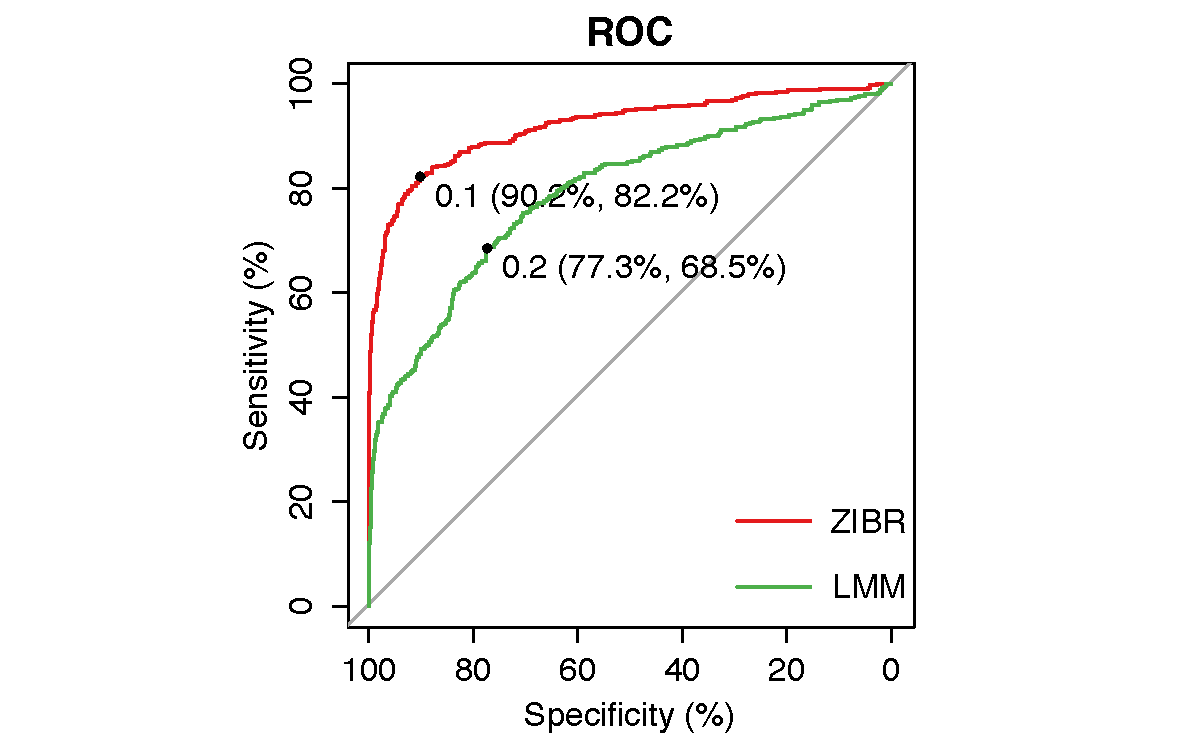
\includegraphics[scale=0.8,trim=0 0 0 0,clip]{Figure/F42_ROC.pdf}}
\caption[ROC curves for identifying association by ZIBR and LMM]{ROC curves for identifying association by ZIBR and LMM, where 1000 species were  simulated and 400 of them had true association with the covariate. The simulations were carried out with $N=50$ subjects and $T=5$ time points for each subject. LMM is the linear mixed effect model with arcsine squared root transformation on the microbial abundance. The best cutoff and the corresponding specificity and sensitivity for each method are indicated, where the best cutoff is defined as the value such that the sum of sensitivity and specificity is the largest.}
\label{Fig2}
\end{figure}

\section{Real data analysis}
We applied ZIBR to a real microbiome study comparing different therapies for pediatric IBD patients \citep{lewis2015inflammation,lee2015comparative}. The study  collected 90 children  with IBD who received one of the three study therapies, including 52 children receiving anti-TNF,
22 receiving exclusive enteral nutrition (EEN) and  16 receiving partial enteral nutrition
with ad lib diet (PEN). Adequate stool samples were available from 86 individuals to
conduct shotgun metagenomic analysis. Gut microbiome samples were
collected at four time points: baseline, 1 week, 4 weeks, and
8 weeks into the therapy.  The bacterial abundances at genus level were  quantified using MetaPhlAn 1.7.6 \citep{segata2012metagenomic}. The low sequencing depth samples and low abundant genus were removed as in \cite{Kostic:2015bh}, \cite{Romero:2014il} and \cite{Stein:2013dl}. After filtering, we had a total of 236 samples with  59 subjects (47 anti-TNF and 12 EEN) and four  time points for each subject as well as 18 most common bacterial genera. Our goal was to identify the bacterial genera that showed overall different abundances over  three time points between  EEN and anti-TNF treatments, adjusting for time effect  and the  abundance at the baseline.  We fitted ZIBR with the baseline abundance, week and treatment as covariates and compared the results  from fitting the linear mixed effect model   \citep{LaRosa:2014kk,Kostic:2015bh} with the same covariates and a subject-specific random effect.   For the LMM, the relative abundance was arcsine squared-root transformed before fitting the model. The linear mixed effect model was fitted using the $lme$ function from $nlme$ package in R. The $p$-values were adjusted using  the Benjamini-Hochberg procedure to control the FDR.  



%%%-------------------------------------------------%%%
%%%------------------------Results------------------%%%
%%%-------------------------------------------------%%%

\begin{table*}[tb]
\begin{center}
\caption[Comparison of results between ZIBR and LMM for four bacterial genera]{Comparison of results between ZIBR and LMM for four bacterial genera, where three covariates, including the baseline abundance, time and treatment, are included in each model. For each genus, the FDR-adjusted $p$-value is shown for each of the three covariates in the model. }\label{tbl2}
\begin{tabular}{lcccccc}
\hline
\multicolumn{1}{l}{} & 	\multicolumn{3}{c}{LMM} & 		\multicolumn{3}{c}{ZIBR}\\		
Species	 &Baseline	&Time	&Treatment &	Baseline&	Time&	Treatment\\
\hline
Lactobacillus&	1.10E-11	&5.68E-02	&4.97E-01	&2.46E-07	&5.38E-01	&9.41E-03\\
Veillonella	&9.04E-07	&8.04E-01	&5.27E-01	&4.81E-07	&9.89E-01	&1.76E-02\\
Collinsella	&2.28E-07	&9.85E-01	&2.91E-01	&6.14E-09	&5.38E-01	&1.57E-02\\
Eubacterium&	1.03E-02&	1.84E-02&	5.04E-02&	1.18E-02&	2.43E-01&	2.67E-02\\
\hline
\end{tabular}
\end{center}
\end{table*}

At FDR=5\%, LMM identified  seven genera, including {\it Ruminococcus}, {\it  Faecalibacterium},  {\it Bifidobacterium}, {\it Dialister}, {\it  Streptococcus}, {\it  Haemophilus} and  {\it  Alistipes}. ZIBR identified all those seven genera and also identified four additional genera, {\it Lactobacillus, Veillonella, Collinsella}, and {\it Eubacterium} (see Figure~\ref{ZibrVenn}). Table \ref{tbl2} shows the FDR-adjusted $p$-value  for each of the three covariates in the model, indicating that the initial abundance of these four genera had large effects for their abundance during the course of the treatment. However, these genera were relatively stable in their abundance during the 8 weeks of treatments. 

After adjusting the baseline abundance, these four genera showed different abundances between anti-TNF and the EEN treatments. 
Figure~\ref{Fig4} shows the abundances of those four genera over time.  {\it Lactobacillus} and {\it Veillonella} were observed more frequently  in the anti-TNF treated group across  different time  points than in the EEN group.  However, no significant difference was observed for the  non-zero abundance when they were observed.   
In contrast, {\it Collinsella} and {\it Eubacterium}  showed  consistent differences across  all three time points in the non-zero abundance but not the frequencies being observed.   Results from ZIBR showed that different treatments led to different  probabilities of observing  {\it Lactobacillus} and {\it Veillonella} (FDR adjusted $p$=0.0049, FDR adjusted $p$=0.0085), but  not   {\it  Collinsella} and {\it Eubacterium} (FDR adjusted $p$=0.299,FDR adjusted $p$=0.50).  In addition, different treatments seemed to  lead to different abundances for  {\it Collinsella} and {\it Eubacterium} (FDR adjusted $p$=0.0254,FDR adjusted $p$=0.0254), but not for  {\it Lactobacillus} and {\it  Veillonella} (FDR adjusted p=0.42, FDR adjusted p=0.93). The advantage of ZIBR is that it considers these two types of differences simultaneously and therefore potentially leads to more power in detecting the differences in abundances between the two treatment groups. 


\begin{figure}[!tpb]%figure3
\centering{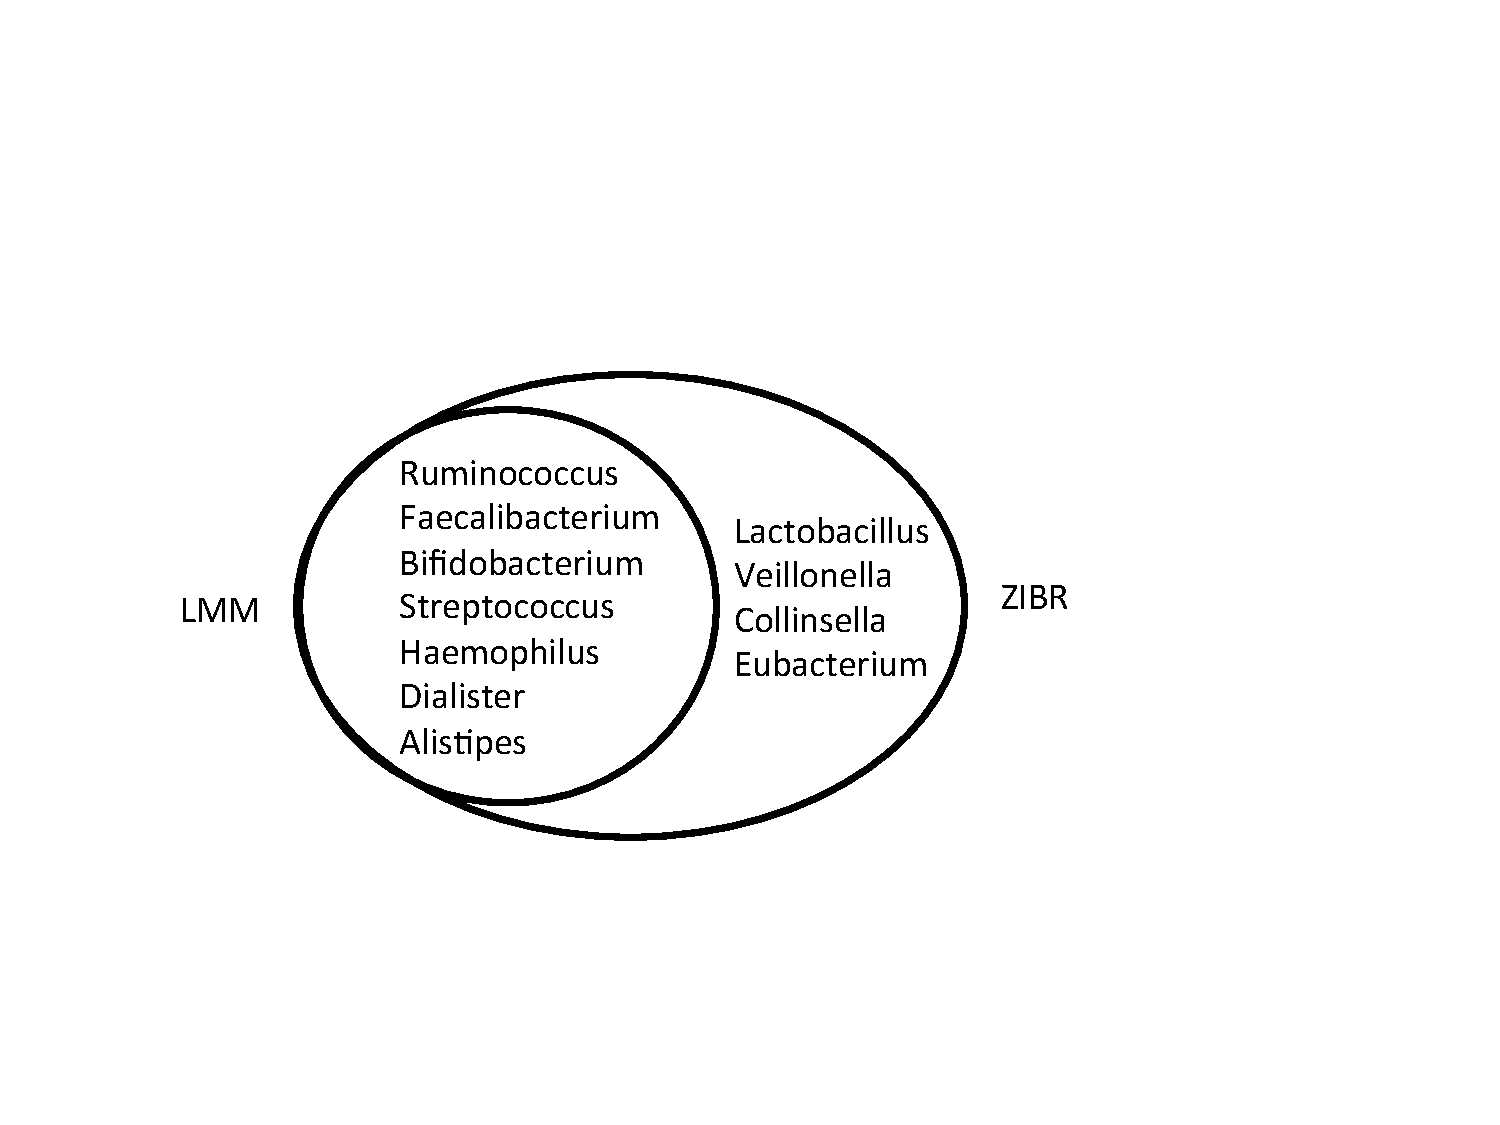
\includegraphics[scale=0.6,trim=20 120 85 150,clip]{Figure/F43_Treatment_Venn.pdf}}
\caption[Bacterial genera that showed  different abundances between anti-TNF and EEN treatments  identified by  ZIBR and LMM]{Bacterial genera that showed  different abundances between anti-TNF and EEN treatments  identified by  ZIBR and LMM after adjusting for the initial abundance.  LMM identified seven genera, which were  also identified by ZIBR. ZIBR  identified additional four genera.}
\label{ZibrVenn}
\end{figure}



\begin{figure}[!tpb]%figure4
\centerline{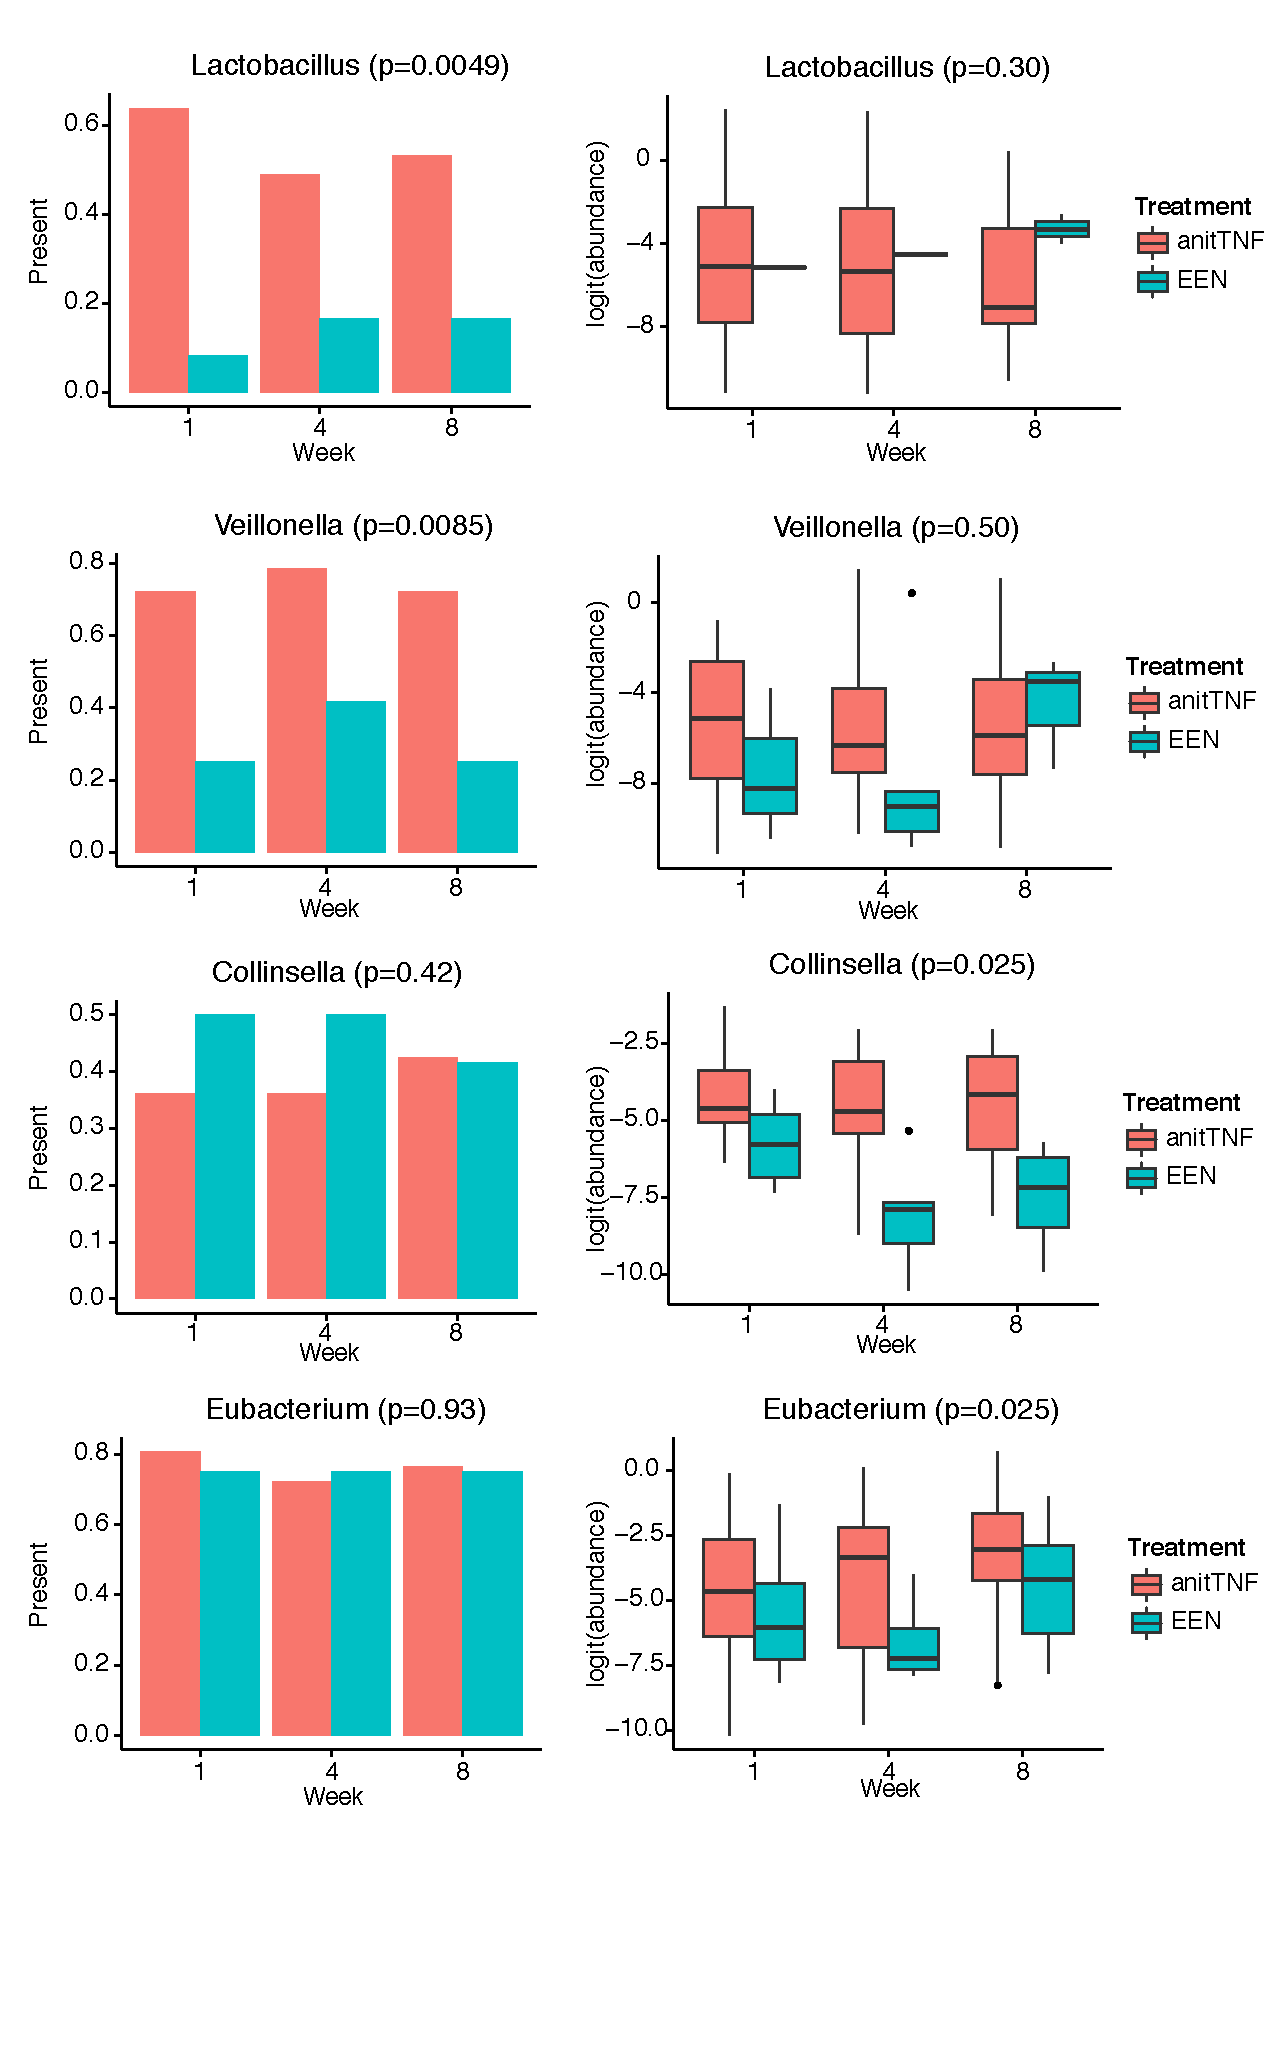
\includegraphics[scale=0.6,trim=0 120 0 0,clip]{Figure/F44_ZIBR_Three_Extra.pdf}}
\caption[Four  genera identified by ZIBR but not by LMM]{Four  genera identified by ZIBR but not by LMM. Left panel shows the percentage of samples in EEN or anti-TNF  groups where the  genus was present. Right panel shows the non-zero abundance in EEN or anti-TNF groups, where the abundances were logit-transformed.}
\label{Fig4}
\end{figure}


\section{Discussion}
We have proposed a two-part mixed-effect model to identify the taxa that are associated with clinical covariates in the longitudinal microbiome studies. Our model takes into account the compositional and sparse nature of the microbiome data as well as the correlation between repeated measures in the longitudinal study.  We  have demonstrated that our proposed model outperforms the commonly  used  linear mixed-effect models.  We  applied our method to the real human microbiome study of  IBD treatment  and identified a number of bacterial genera  that showed different abundances between two commonly used treatments during the eight-week treatment period. 

In our simulations  and analysis of real data, te ZIBR model  involves the same covariates for logistic regressions and Beta regression.  However, our model is more flexible, which  can include  multiple   covariates and different covariates  in two different  components of the model.  Besides identifying bacterial taxa, the model proposed here can also be applied  to identify microbial genes or pathways that show different profiles  in longitudinal microbiome studies.



%% -------------- Reproducible --------------%%
\chpt{Reproducible research}\label{chpt:repro}

The concept of reproducible research has been  advocated by more and more researchers in the scientific community \citep{Peng:2011et, Sandve:2013gh}. The idea of reproducible research is that any computational results the researchers generate, such as numbers, figures, tables, etc., can be re-generated with minimal effort by themselves and other researchers. This is especially necessary for computational and big data research. The computational analysis usually involves  multiple steps of data preprocessing and the statistical models and computational tools used in the analysis often involve many parameters.   The analysis procedure, statistical models and computational tools need to be validated and reproduced by other researchers. 

One interesting and effective  idea in reproducible computational research is to use literate programming. Simply put, literate programming is to organize the code with results and annotations together in just one file. In R, one can generate this type of file with RMarkdown (or knitr) package. In Python, one can do this with IPython Notebook. Since R is mainly used for the analysis in this dissertation,  RMarkdown was used as the tool for reproducible research. The output of RMarkdown reports can be PDF, Word or HTML format. HTML format can be distributed easily so that researchers can view it in the regular web browser.  All the analyses  in this dissertation are reported in HTML format. Figure~\ref{F61_Reproducible_Research} shows an example of the RMarkdown report in HTML format. The code and corresponding results such as figures and tables are integrated together in one report. The code along with the parameters and options are demonstrated above the results. Researchers who want to repeat the analysis can rerun the same code.



\begin{figure*}[p]
	\centering
	{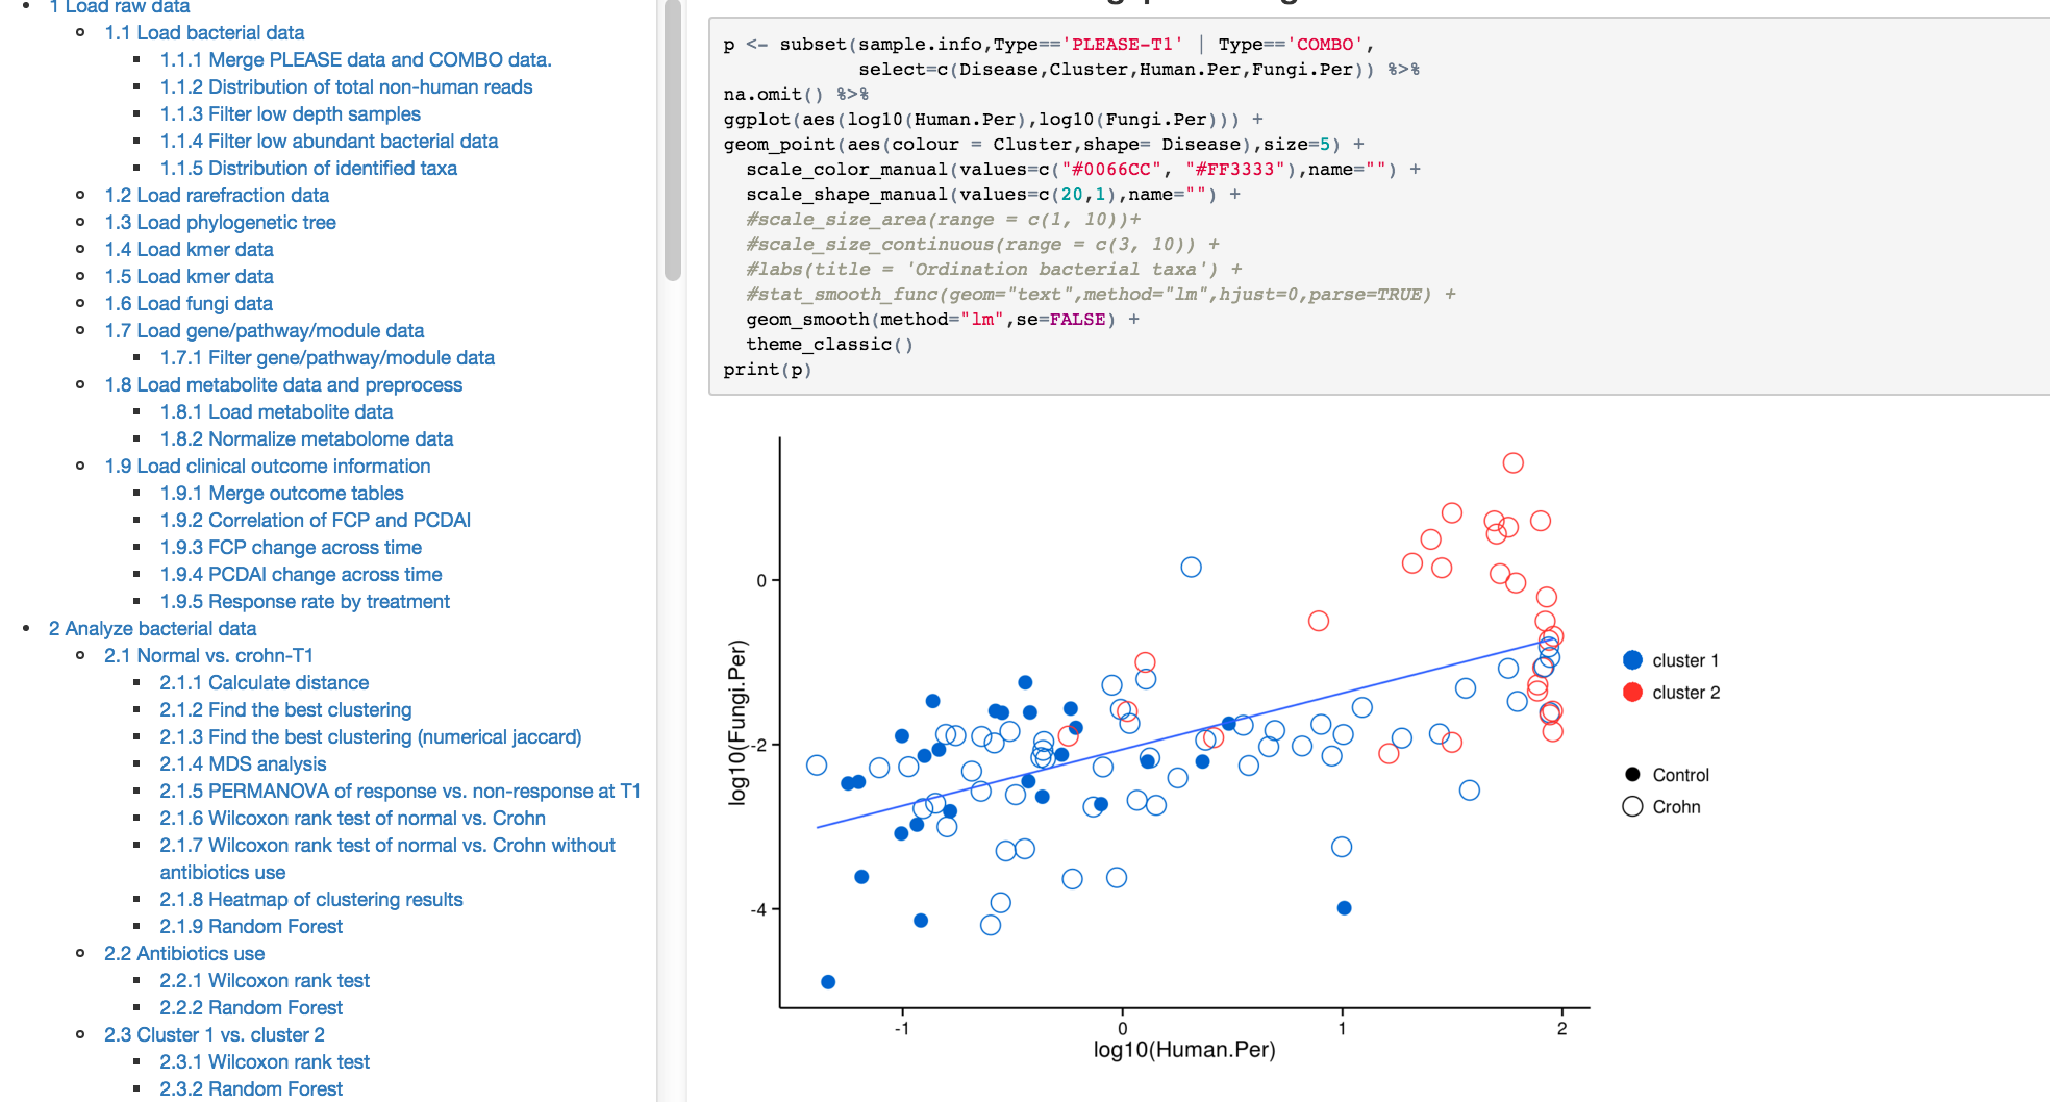
\includegraphics[scale=0.4,trim=0 0 0 0,clip]{Figure/F61_Reproducible_Research.pdf}}
	\caption[An example of RMarkdown report]{An example of Rmarkdown report. The RMarkdown integrates R code, analysis output such as numbers, figures, tables, and annotation text. The analysis in the RMarkdown report is organized and indexed by an index table.  All the analyses included in this dissertation were implemented as RMarkdown reports.
	}
	\label{F61_Reproducible_Research}
\end{figure*}


To make sure that all the statistical models proposed in this dissertation can be easily applied by other researchers in their research, I implemented the statistical models in R packages and made them  available in Github (Figure~\ref{Github_MSSQ}). Github is freely accessible to public users and it is easy to install R package directly from Github. In this way, researchers do not need to implement the proposed statistical models by themselves. Users who identify bugs in the package or have any improvement suggestions can comment on the corresponding  package website. 

\begin{figure*}[p]
	\centering
	{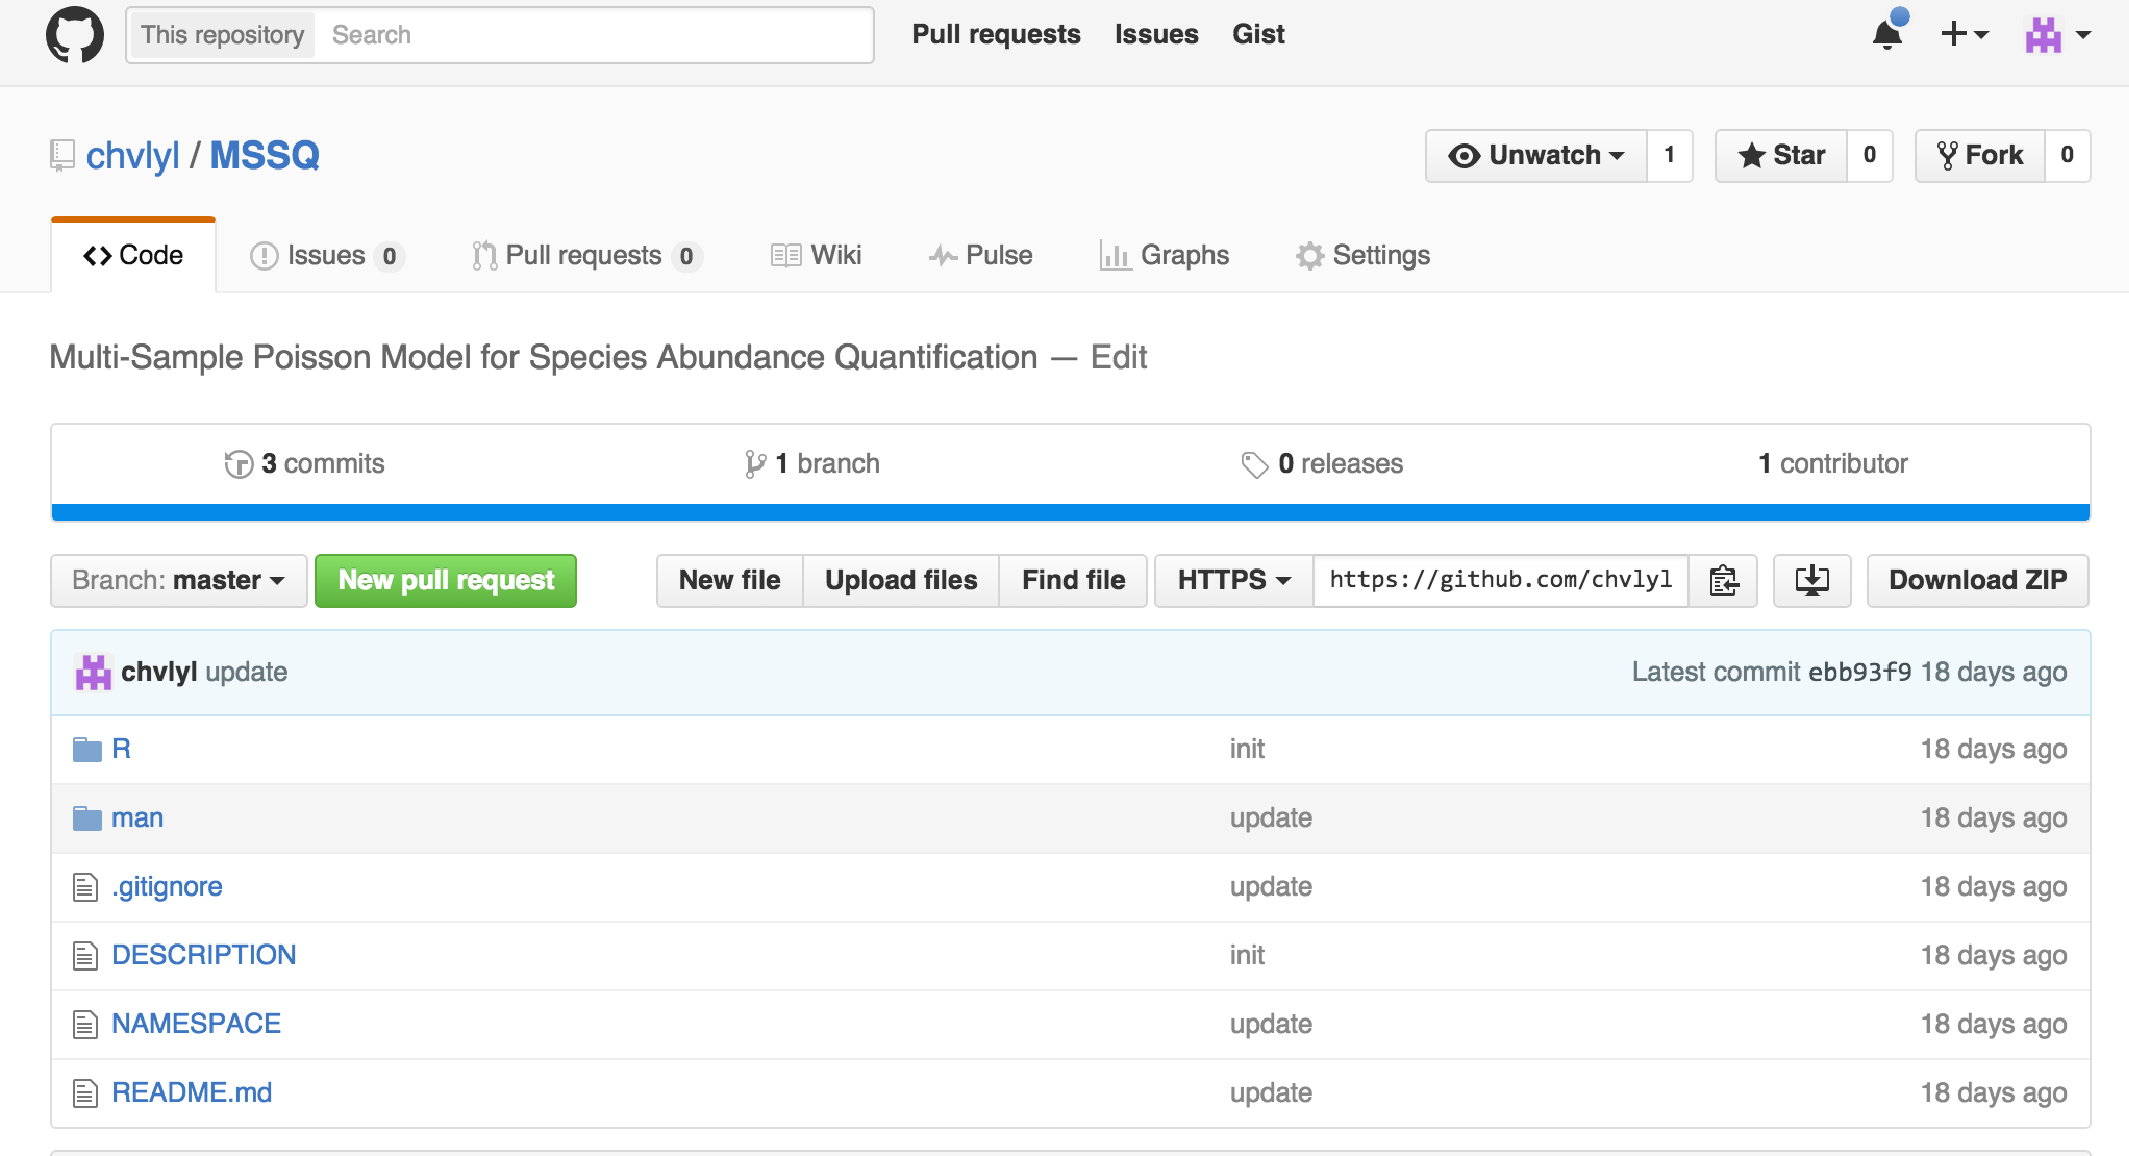
\includegraphics[scale=0.4,trim=0 0 0 0,clip]{Figure/F62_Github_MSSQ1.pdf}
	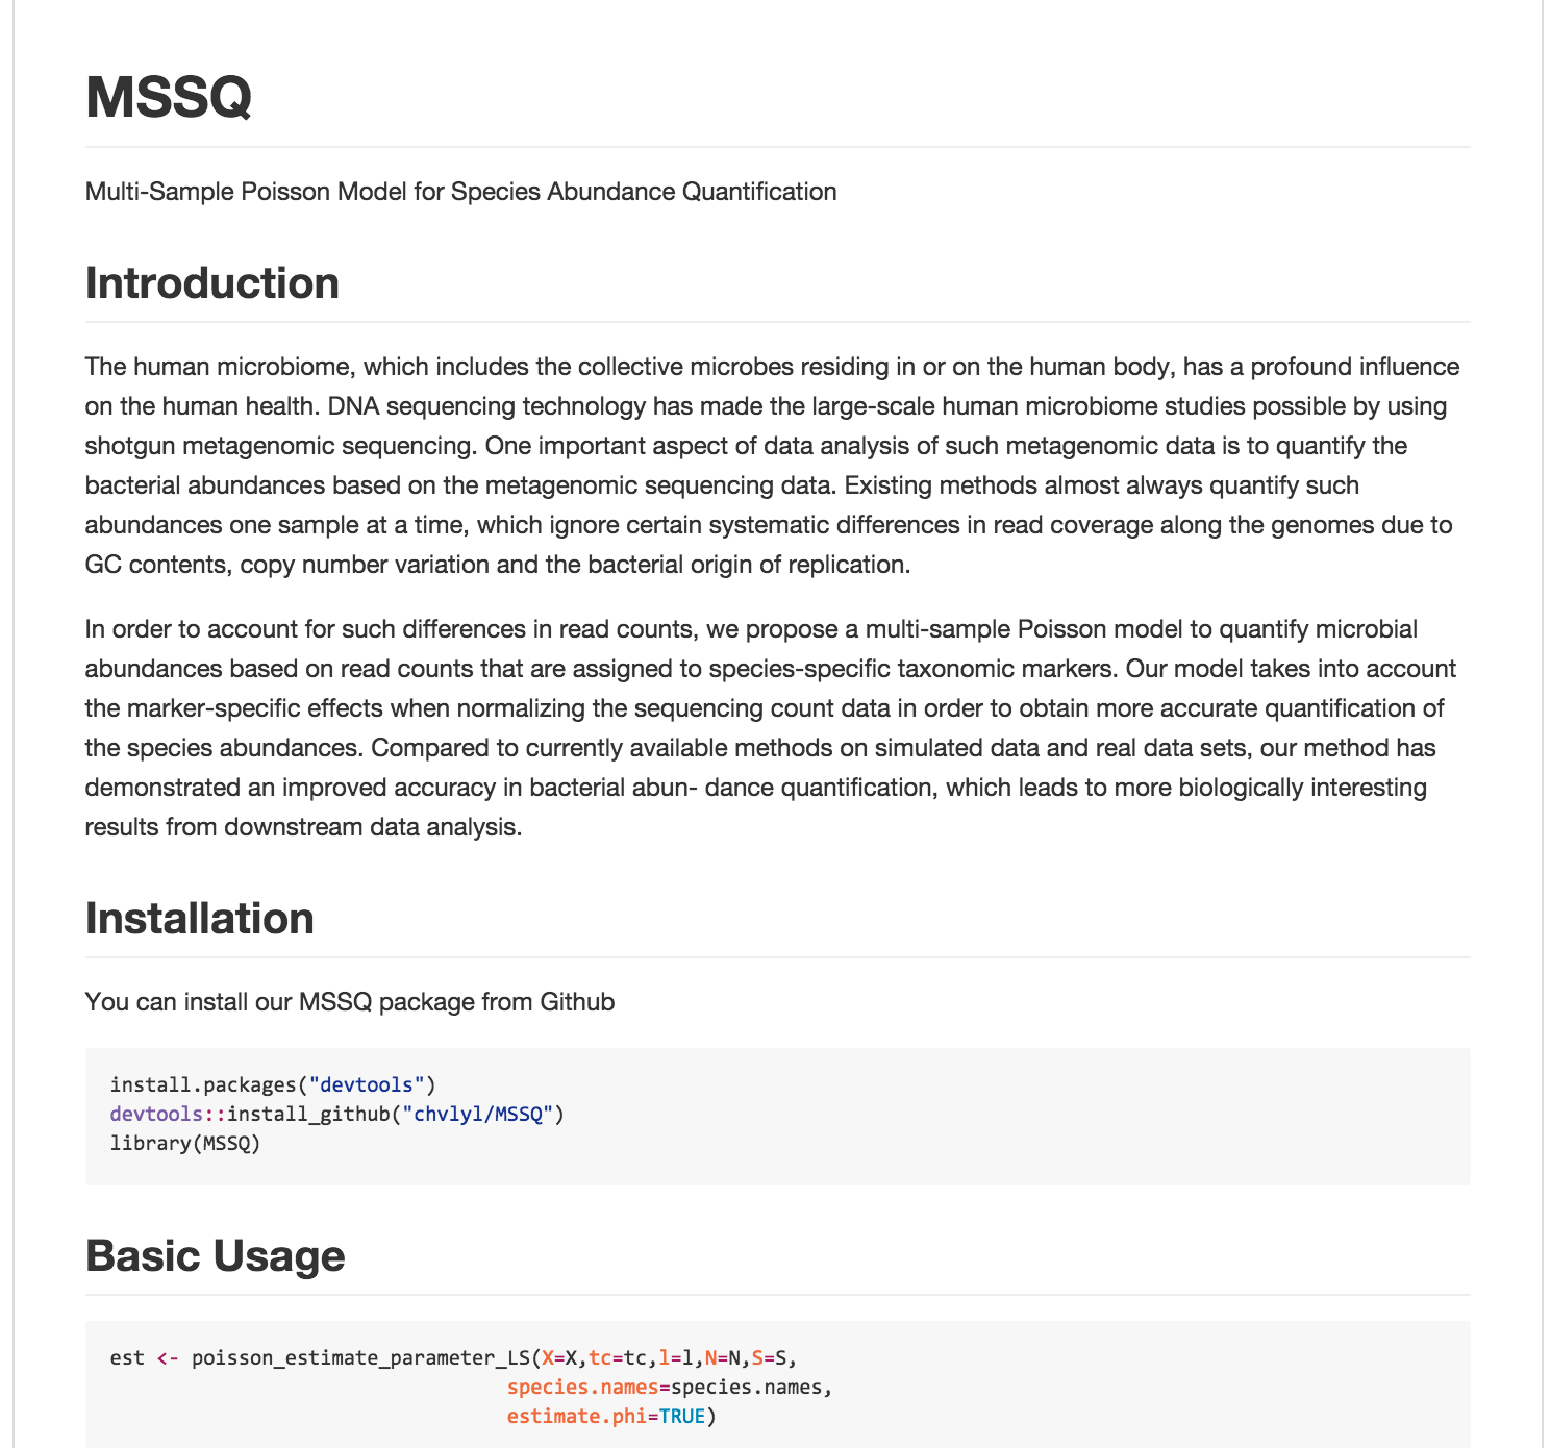
\includegraphics[scale=0.4,trim=0 0 0 0,clip]{Figure/F63_Github_MSSQ2.pdf}
		
	}
	\caption[An example of R packages distributed on Github]{An example of R package MSSQ on Github. Researchers who are interested in using this package can easily install it from Github. All the code are freely available to the public users. An instruction of the package is also included at the main website of this package. Another R package ZIBR introduced in this dissertation was also submitted to Github in a similar fashion.
	}
	\label{Github_MSSQ}
\end{figure*}


Some analyses are also implemented in interactive web applications with R Shiny (Figure~\ref{F64_Shiny}). Users can explore the analyses and results  by simply changing certain parameters. The figures are then  automatically updated. This is especially useful in exploratory statistical analysis that researchers want to investigate  certain  analysis using  different parameter settings.


\begin{figure*}[p]
	\centering
	{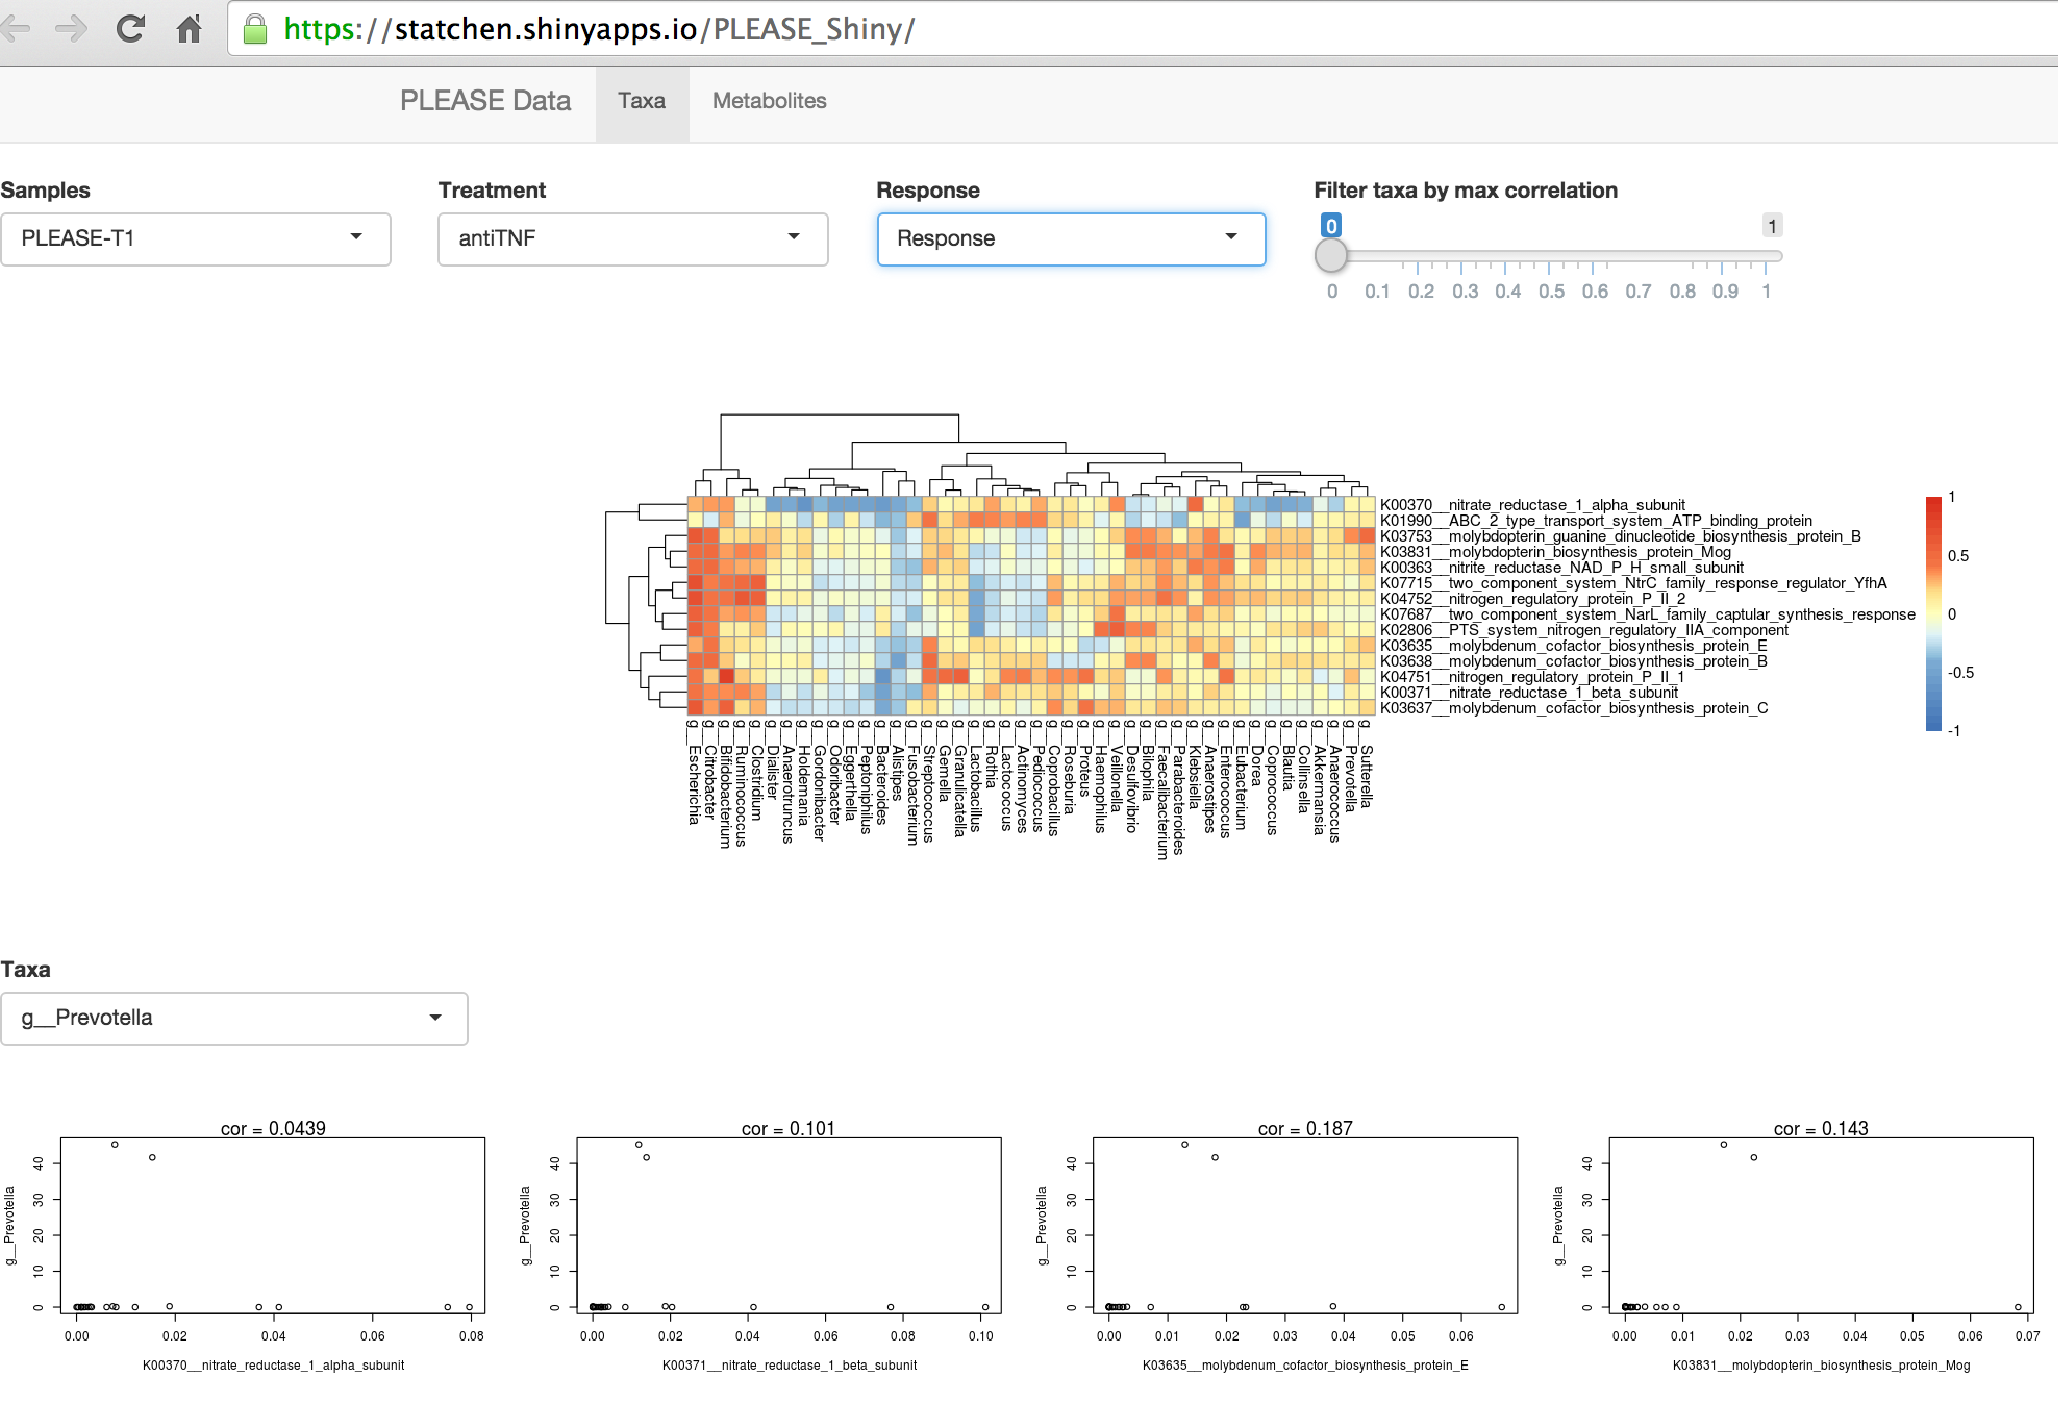
\includegraphics[scale=0.4,trim=0 0 0 0,clip]{Figure/F64_Shiny.pdf}
	}
	\caption[An illustration of interactive analysis of microbiome data]{An illustration of interactive analysis of microbiome data. Users can analyze and visualize the correlations between metabolites and bacterial taxa in different groups. Users  can also filter out the taxa with low correlations. The figure is  automatically updated after users change the setting. This interactive web application was implemented with R Shinny. 
	}
	\label{F64_Shiny}
\end{figure*}


%% -------------- Discussion --------------%%
\chpt{Conclusion and future work}\label{chpt:discussion}

This dissertation presents three projects related to the human microbiome. The first project presents the Penn microbiome study of pediatric Crohn’s disease. By analyzing the microbiome data and clinical data from a prospective cohort of pediatric Crohn’s disease patients, we revealed the full complement and dynamics of bacteria and fungi associated with Crohn’s disease and treatment. The second project proposes a multi-sample Poisson model to quantify microbial abundances based on the shotgun metagenomic data. The third project presents another statistical model for association analysis of longitudinal microbiome data. The work provides new insight into the role of human gut microbiome in Crohn’s disease. The statistical models proposed in this dissertation also provide new computational tools for microbiome data analysis. However, microbiome is still a relative new and challenging research area. Following are some future work that need further exploration.

\section{Integration of metabolomic data with metagenomic data to further understand Crohn's disease}
The work presented in the dissertation focused on analysis of microbiome data in order to understand the dysbiosis in Crohn's disease. We have demonstrated that the dysbiosis is caused by multiple factors such as inflammation, antibiotic use and diet. However, the detailed mechanism of dysbiosis development in Crohn's disease is still undetermined. In order to address this question, we also generated metabolomic data from the fecal same samples in the previous study. 
Figure~\ref{F54_Metabolites_Heatmap} shows a global profile of the metabolites in control and Crohn's disease samples.  The clustering of samples and metabolites shows some interesting patterns. For example, the carnitines such as C5 carnitine and C9 carnitine are positively correlated with disease status (control vs. Crohn) and disease activity indicated by FCP values.  We applied the Random Forest model to predict the control and Crohn's disease samples with known metabolite abundance (Figure~\ref{F53_Metabolites_RF}). The out-of-bag prediction accuracy is 89\% and the most important metabolites are lipids as well as carnitines. These preliminary results from the metabolomic data analysis indicate that the lipids especially carnitines may play critical role in dysbiosis in Crohn's disease. By integrating metabolomic data with metagenomic data such as microbial abundance and gene pathway abundance, as well as clinical data, we can investigate the association among metabolites, bacteria, fungus, disease activity. It is interesting to know how this association can shed light on novel diagnostic and therapeutic procedures for Crohn's disease. 


\begin{figure*}[hp]
\centering
{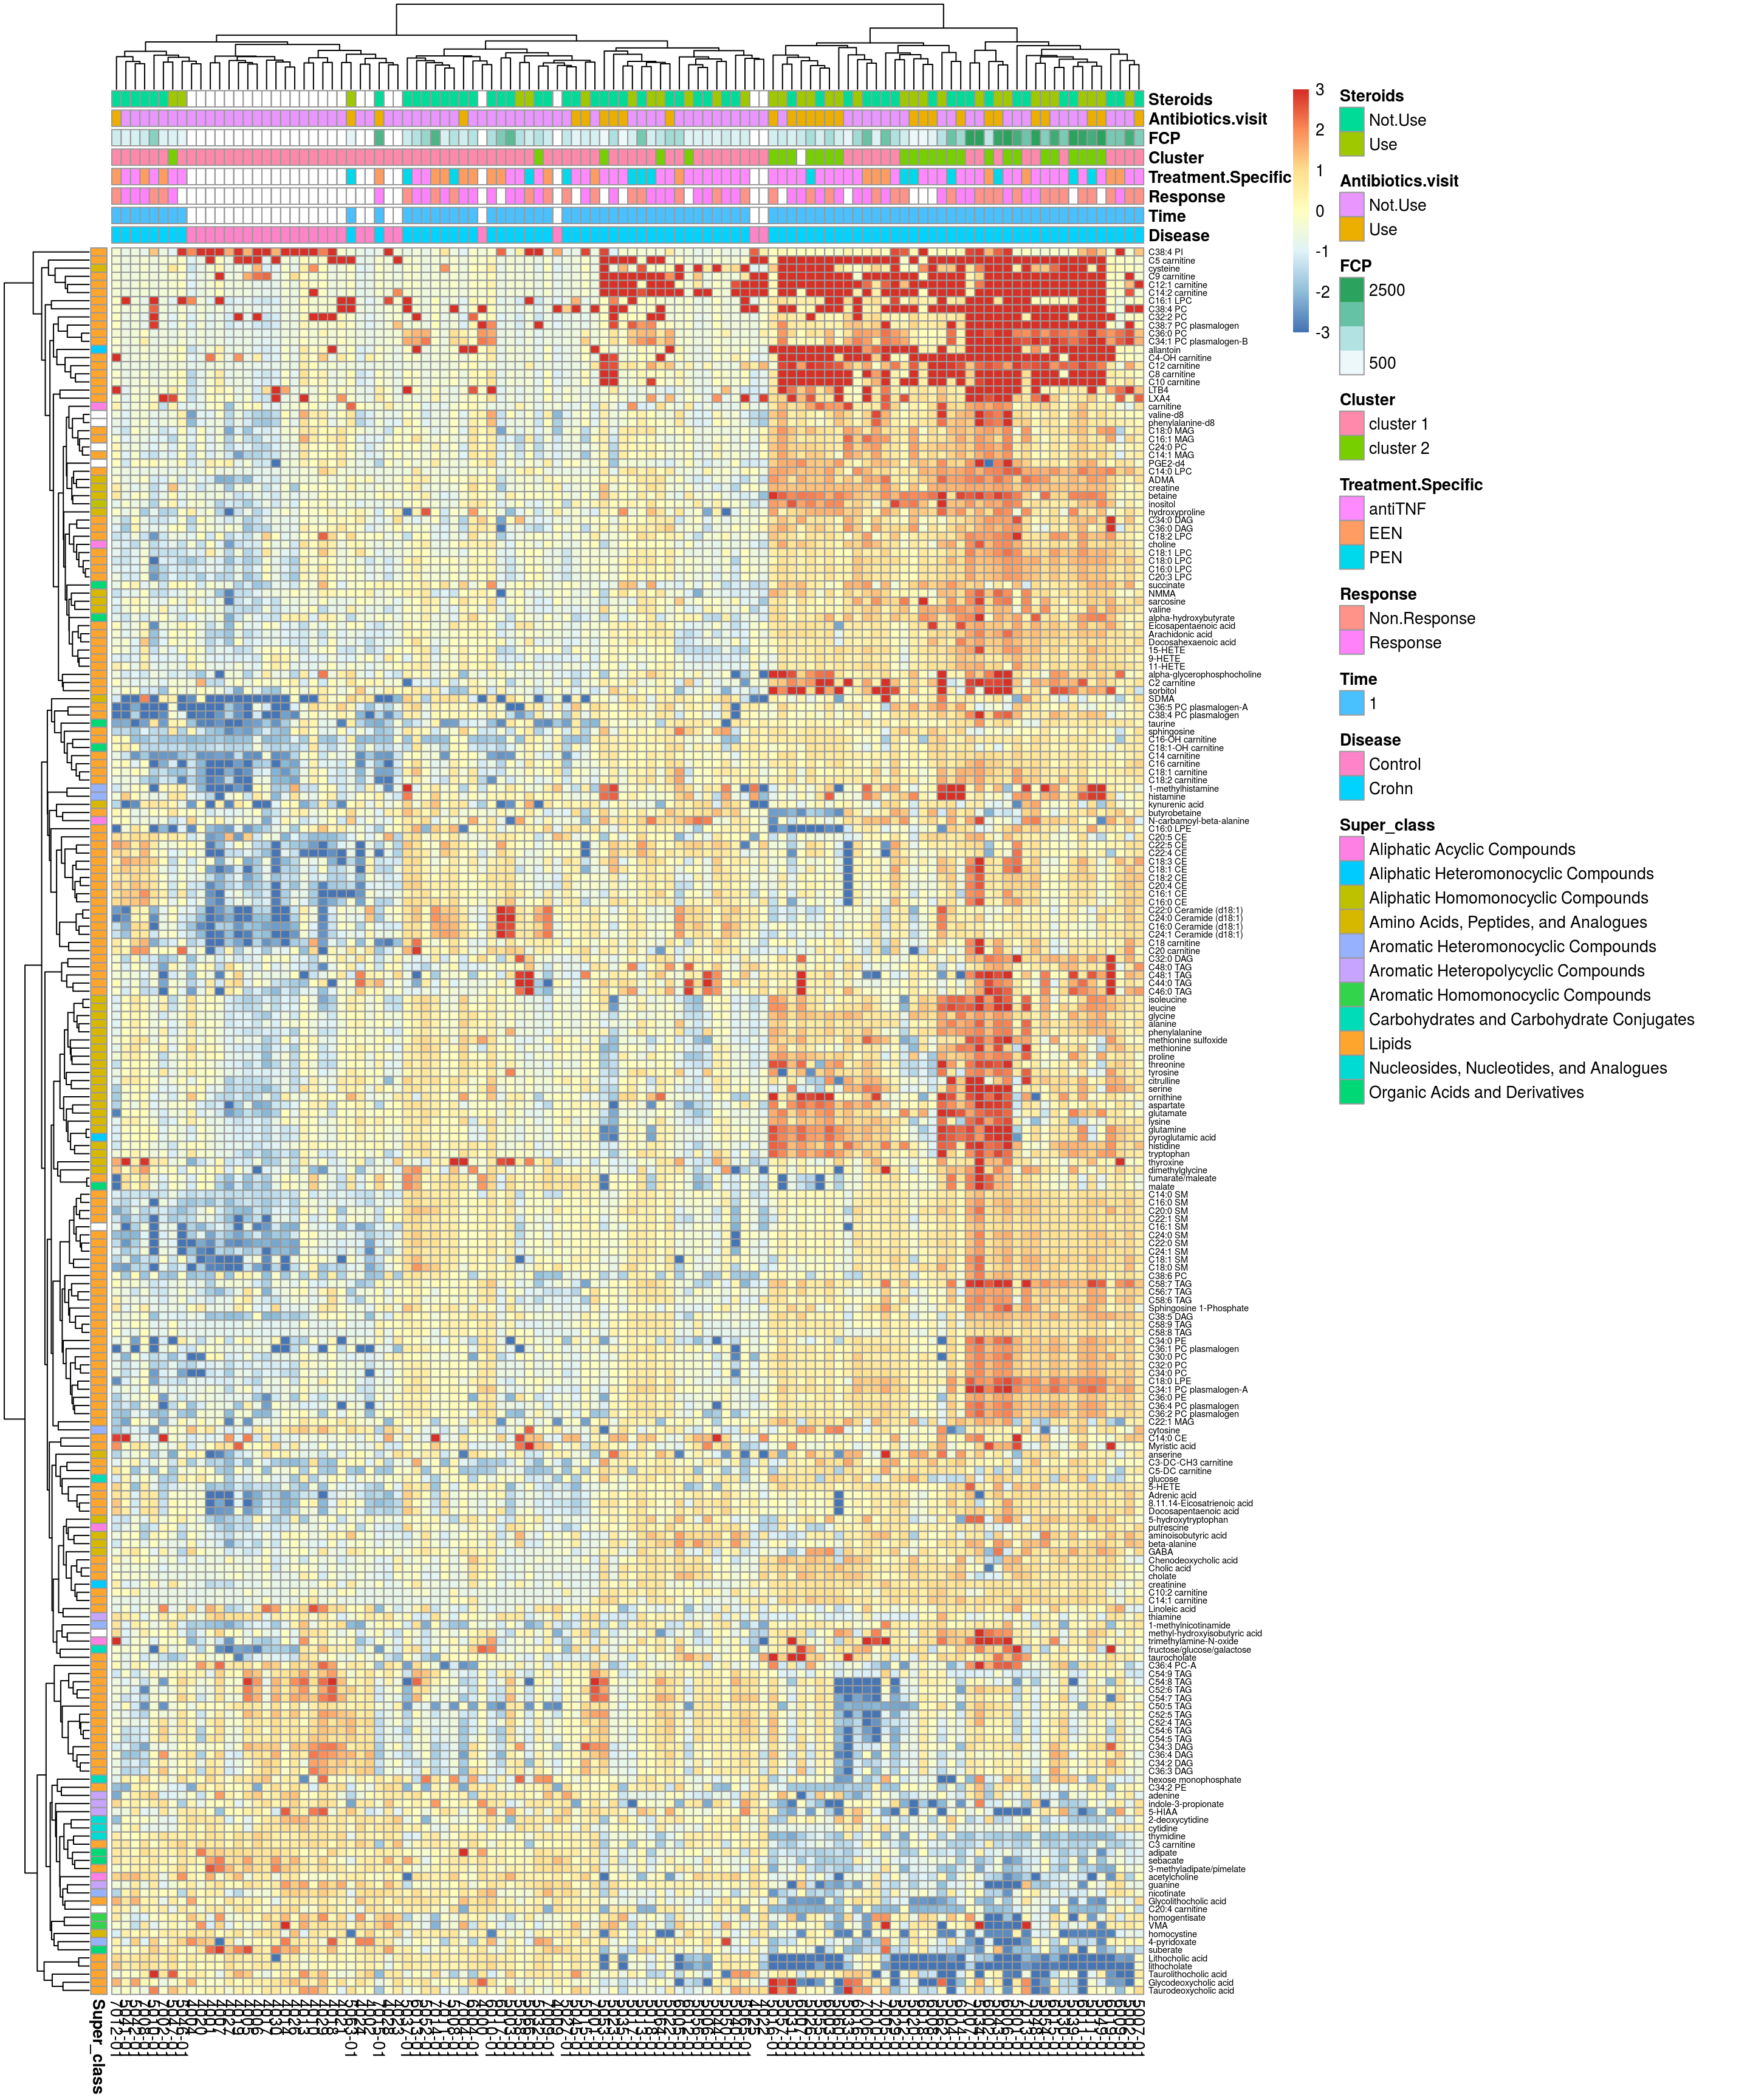
\includegraphics[scale=0.4,trim=0 0 0 0,clip]{Figure/F54_Metabolites_Heatmap.png}
}
\caption[A heatmap demonstrating the relative abundance of known metabolites]{A heatmap demonstrating the relative abundance of known metabolites in control and disease samples at baseline. Metadata are indicated by the color code at the top of the figure. The metabolites are grouped into several classes and indicated by the color code on the left side of the figure. Only metabolites that show differential abundance between control and disease samples at baseline are plotted in the heatmap, which are defined by q value $<$ 0.05 with Wilcoxon rank-sum test}
\label{F54_Metabolites_Heatmap}
\end{figure*}



\begin{figure*}[hp]
\centering
{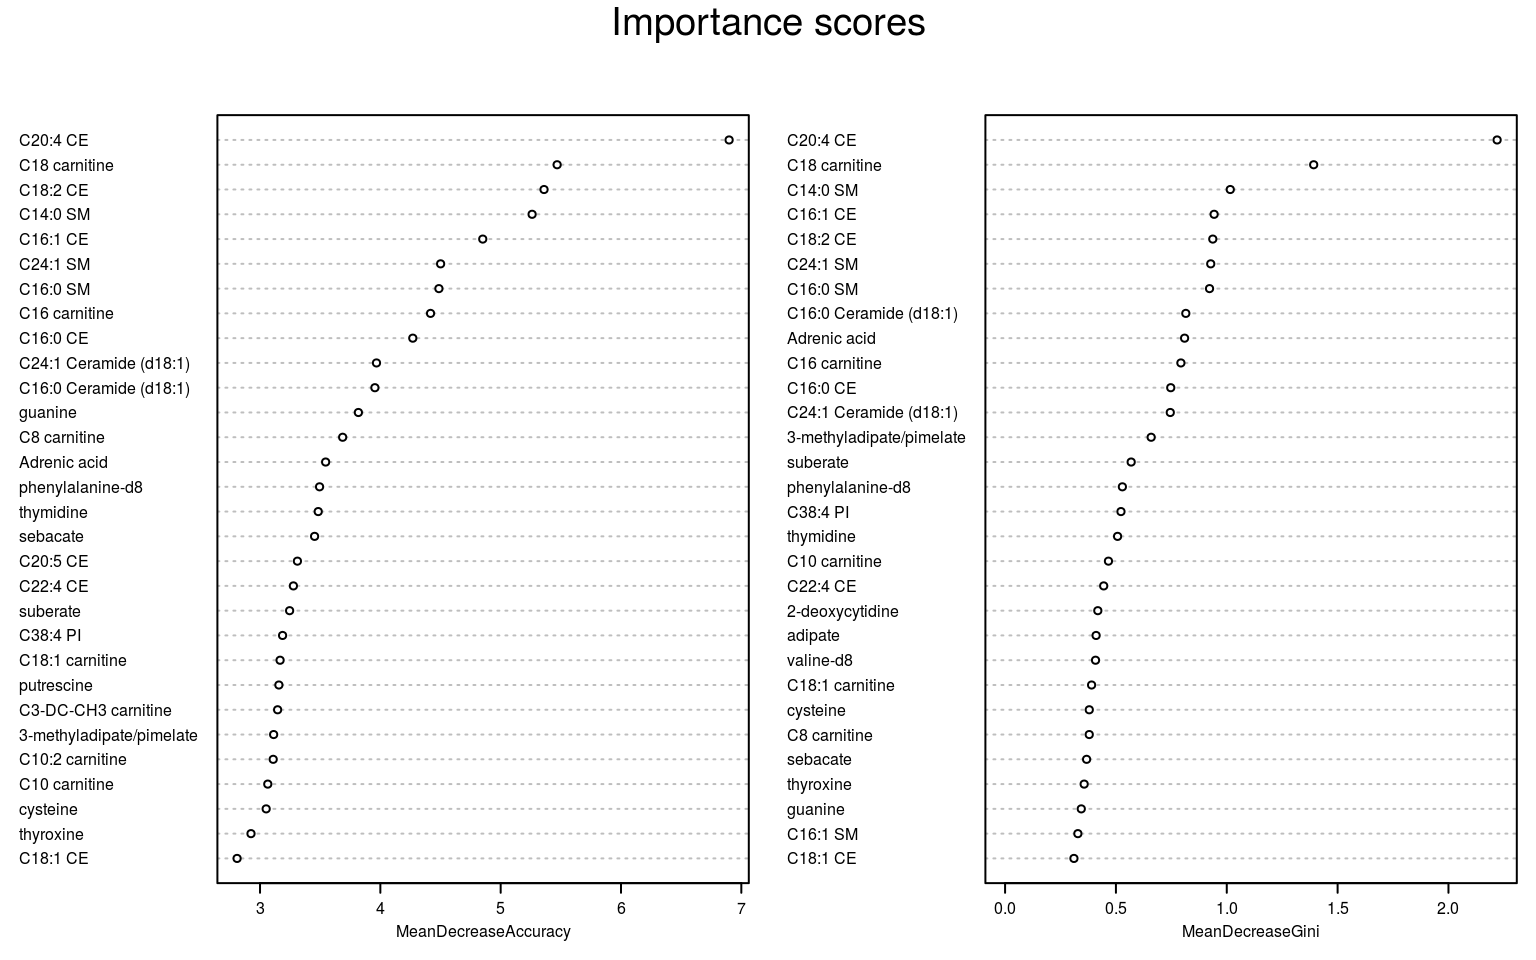
\includegraphics[scale=1.2,trim=0 0 290 30,clip]{Figure/F53_Metabolites_RF.png}
}
\caption[Prediction of control and Crohn's disease samples using known metabolites by Random Forest]{Prediction of control and Crohn's disease samples using known metabolites by Random Forest. The metabolites are ranked by Random Forest so that the top ones are most important in predicting control versus disease samples. Control and Crohn's disease samples at baseline were used in the Random Forest analysis. 
}
\label{F53_Metabolites_RF}
\end{figure*}


\section{Analysis of microbiome data with k-mers} 
The shotgun metagenomic data is challenging to analyze because many similar microbial genomes are presented in the sample and thus it is difficult to sort the sequencing reads back to the reference genome. Currently, the most popular approach for shotgun metagenomic data analysis is to utilize marker genes, either taxa specific markers or universal markers, as alignment reference. This approach has been well adapted and widely applied in shotgun metagenomic studies. However, since those markers are only a small subset of the microbial genomes, thus only a small proportion of the sequencing reads can be aligned to the markers. Thus majority of the data are discarded because they are originally generated from the non-marker genomic regions. 

One alternative approach for shotgun metagenomic data analysis is to make use of k-mers. That is, we can split the sequencing reads into k-mers, say 6mers, and count the k-mer frequency in the sample. The k-mer frequency could be potentially informative. To test this idea, we generated 6mers from the shotgun metagenomic data used in the previous analysis after removing human reads and low quality reads.  The  frequency of each 6mer was counted and then normalized into relative abundance so that the abundance of all 6mers in one sample sums to one. We then applied Random Forest to predict control and Crohn's disease samples using 6mer relative abundance. The out of bag prediction accuracy is 85\% using 6mers and the top six 6mers that are most important to prediction accuracy are plotted in Figure~\ref{F55_Kmer_Difference}. The 6mers such as TACAAC and AAGCTT show significant differential abundance between control and Crohn's disease samples. It is interesting to further explore why those 6mers are associated with disease status. Testing the association between the 6mer abundance and other clinical variables such as FCP values and response status to the treatments is another future research direction. 

More advanced and rigorous statistical models need to be developed for the analysis of k-mers from shotgun metagenomic data. One possible research direction is to apply the topic model on k-mer data. The topic model is a class of statistical models to identify the hidden topics in a collection of documents. In this case, we can consider each sample as a document and k-mers as words in the document. By using topic models, we can identify the hidden biological structure in the data. 

\citet{taddy2013multinomial} introduced a multinomial inverse regression to model the word frequency in the document and derive low dimension representations.
\begin{equation*}
X_y \sim Multinomial(q_y,m_y),
\end{equation*}
where $q_{yj} = \frac{exp(\alpha_j+\beta_jy)}{\sum_{l=1}^{p}exp(\alpha_l+\beta_ly)}$,
$m_y = \sum_{i:y_i=y}m_i$.
Here, $y$ is the index for documents. $X_y$ is the word frequency and $m_y$ is the total word counts. For details of this model, readers can refer to \citet{taddy2013multinomial}.
The number of unique words in the documents usually is very large and thus we are facing a high dimensional regression problem. The dimensions  can be reduced through sufficient reduction (SR) and it can be calculated as 
\begin{equation*}
z_i = \beta'f_i,
\end{equation*}
where $f_i = \frac{x_i}{m_i}$.
The SR score is shown to correlate with main theme of the data such as restaurant rating score \citep{taddy2013multinomial}. 

We applied the multinomial inverse regression model to the k-mer data generated from control and Crohn's disease samples. We first extracted 6mers from the shotgun sequencing reads after removing human reads and low quality reads and then counted the frequency of each unique 6mer. We fitted the multinomial inverse regression model and calculated the SR score for each samples. Figure~\ref{F51_SR_control_disease} shows that the SR scores generated from 6mer data are associated with disease status. We further stratified  the Crohn's disease samples into antibiotic use and non-use groups (Figure~\ref{F52_SR_control_disease_antibiotics}). The Crohn's disease samples with antibiotic use show higher SR score than control samples and Crohn's disease samples without antibiotic use.

Although it is inspiring  and promising to see the association between SR score summarized from 6mers and clinical variables such as disease status and antibiotic use, there are still many unsolved  issues. First, different from words in the documents, the k-mer data generated from metagenomic data have several unique features.  Due to the sequencing error, the observed k-mers that originate from the same genomic region may have different sequences. Also, the metagenomic data are mixture of sequencing reads from microbial genomes and human genomes. However, none of the currently available topic models take into account those unique features in the metagenomic data. Thus, developing a topic model that handles these problems is quite necessary. Second, the longer the k-mer, the more informative it would be. For example, in the current analysis, we use 6mers. However, longer k-mers such as k=30 are more biologically informative. But k=30 will generate $1.152922\times 10^{18} $ unique 30mer sequences. It is very computationally challenging to model such data. Therefore, statistical models and computational algorithms for analyzing such ultra-high dimensional data are worth exploring. Third, the topic models can identify  topics with corresponding  theme words. In the k-mer case, how to interpret the biological topics and how to functionally  annotate k-mers in each topic are not clear. 

 

\begin{figure*}[p]
	\centering
	{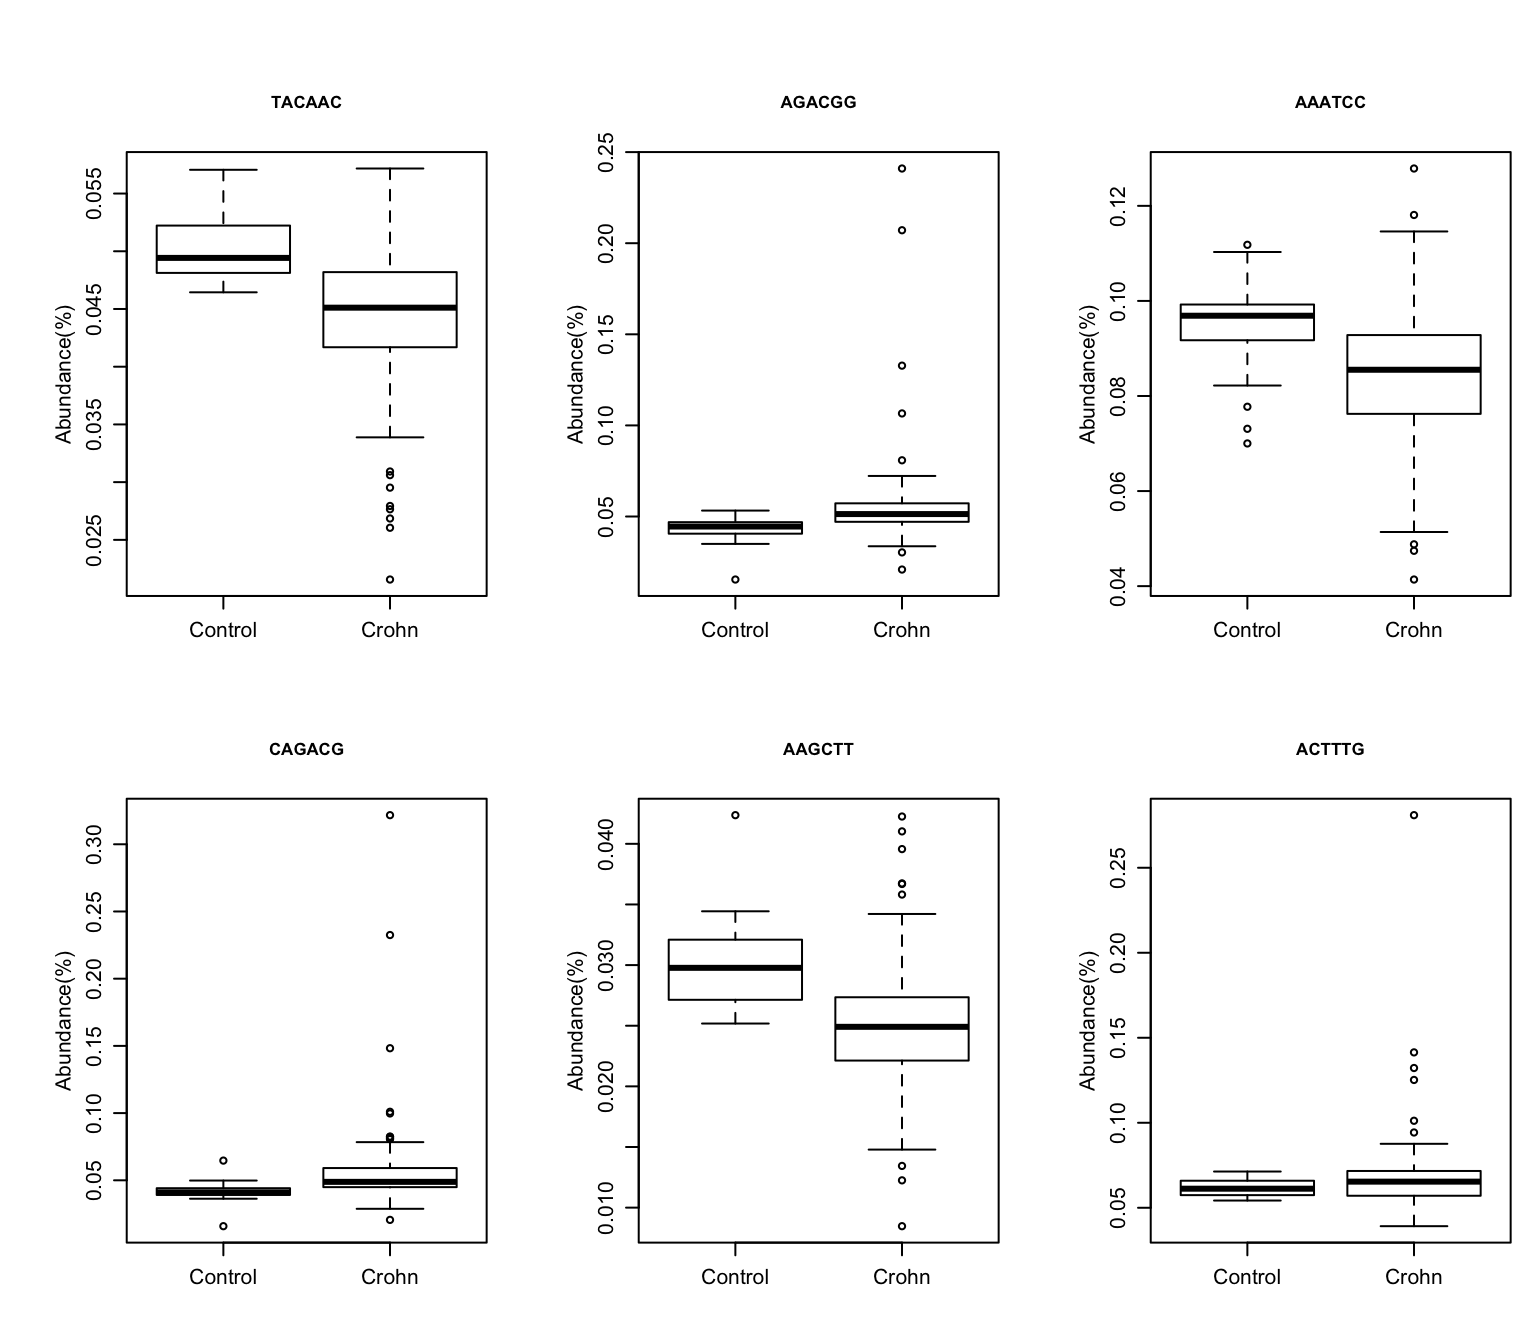
\includegraphics[scale=0.28,trim=40 0 0 0,clip]{Figure/F55_Kmer_Difference.png}
	}
	\caption[Comparison of control and Crohn's disease samples with 6mers]{Comparison of control and Crohn's disease samples with 6mers. The 6mers were generated from the shotgun metagenomic data used in the previous analysis after removing human reads and low quality reads. The  frequencey of each 6mer was counted and then normalized into relative abundance so that the abundance of all 6mers in one sample sums to one. Random Forest was then applied to predict control and Crohn's disease samples using 6mer relative abundance. The top six 6mers that are most important to prediction accuracy are plotted. The 6mer sequences are indicated at the top of each plot.
	}
	\label{F55_Kmer_Difference}
\end{figure*}





\begin{figure*}[p]
\centering
{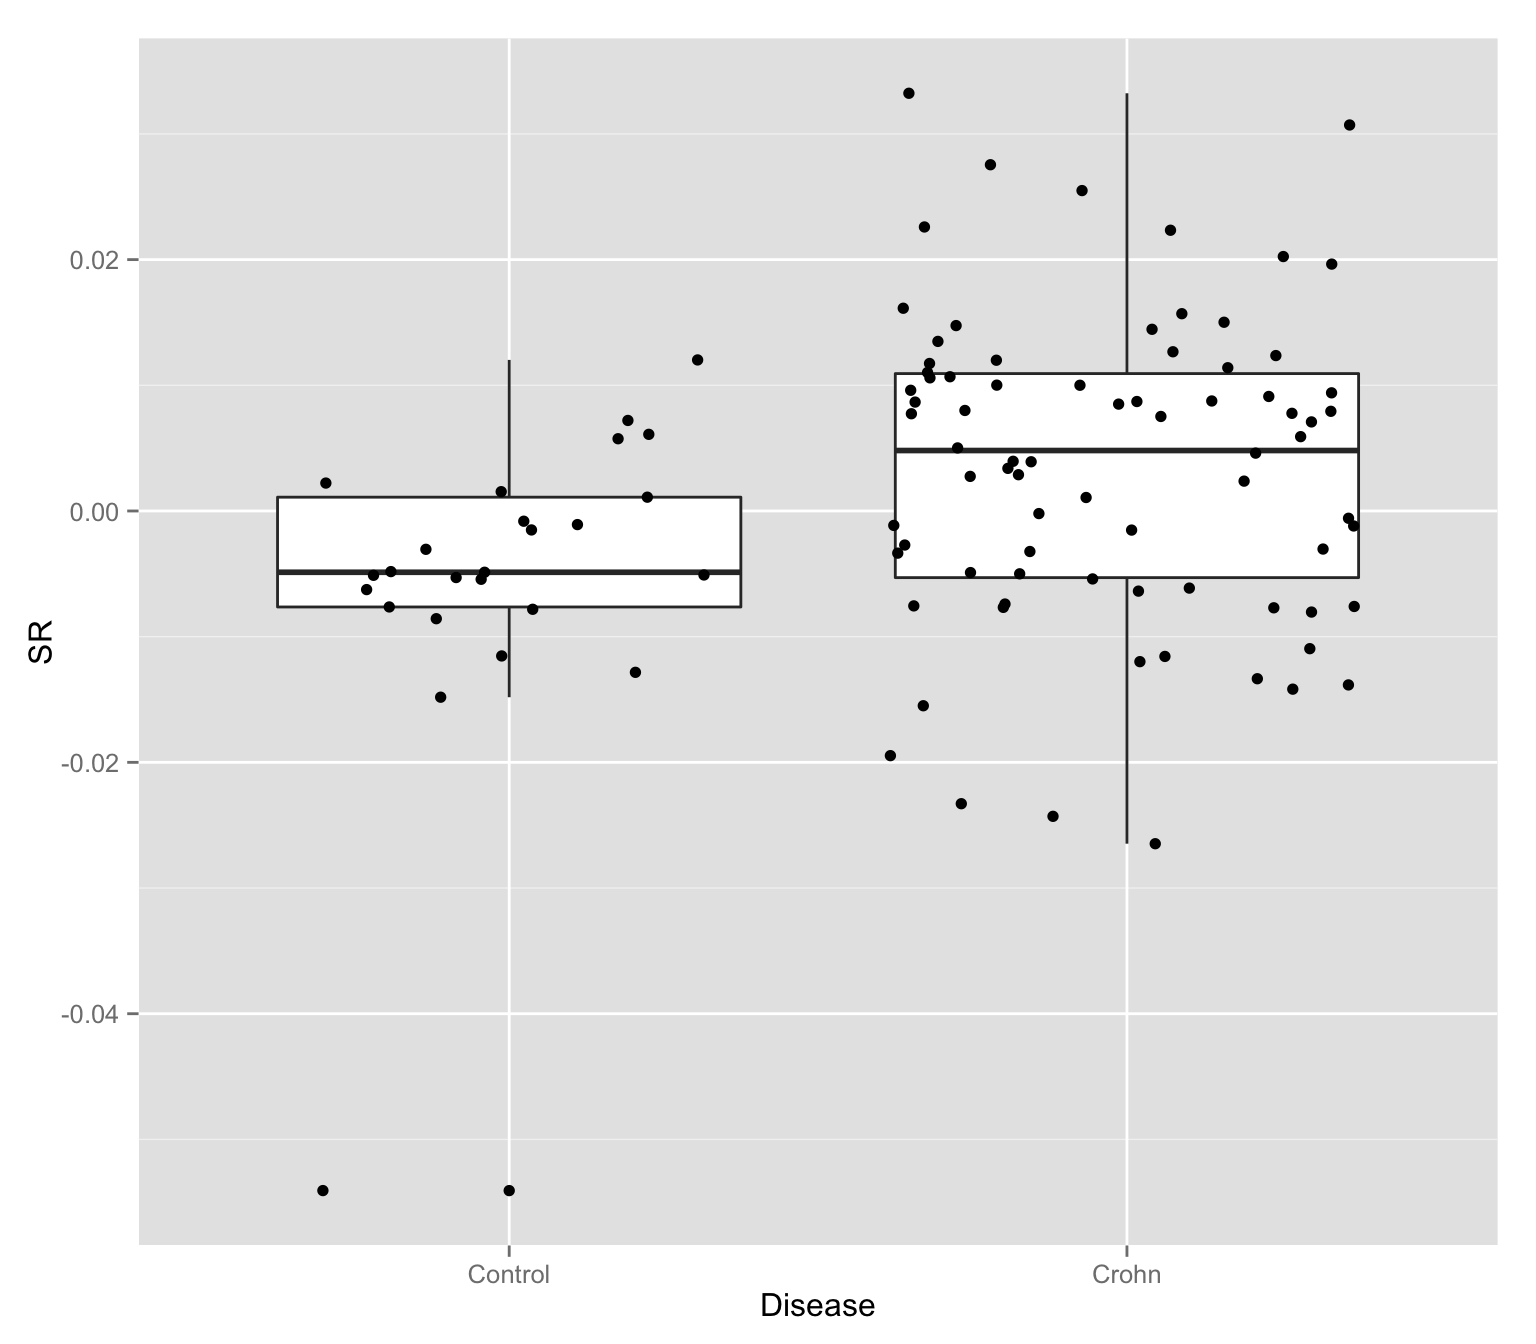
\includegraphics[scale=0.25,trim=0 0 0 0,clip]{Figure/F51_SR_control_disease.png}
}
\caption[Comparison of control and Crohn's disease samples with SR score]{Comparison of control and Crohn's disease samples with SR score. K-mers (k=6) were extracted from the shotgun sequencing reads and the frequency of each k-mer was counted. Then multinomial inverse regression model was fitted to the k-mer count data and the sufficient reduction (SR) score was calculated.   
}
\label{F51_SR_control_disease}
\end{figure*}



\begin{figure*}[p]
\centering
{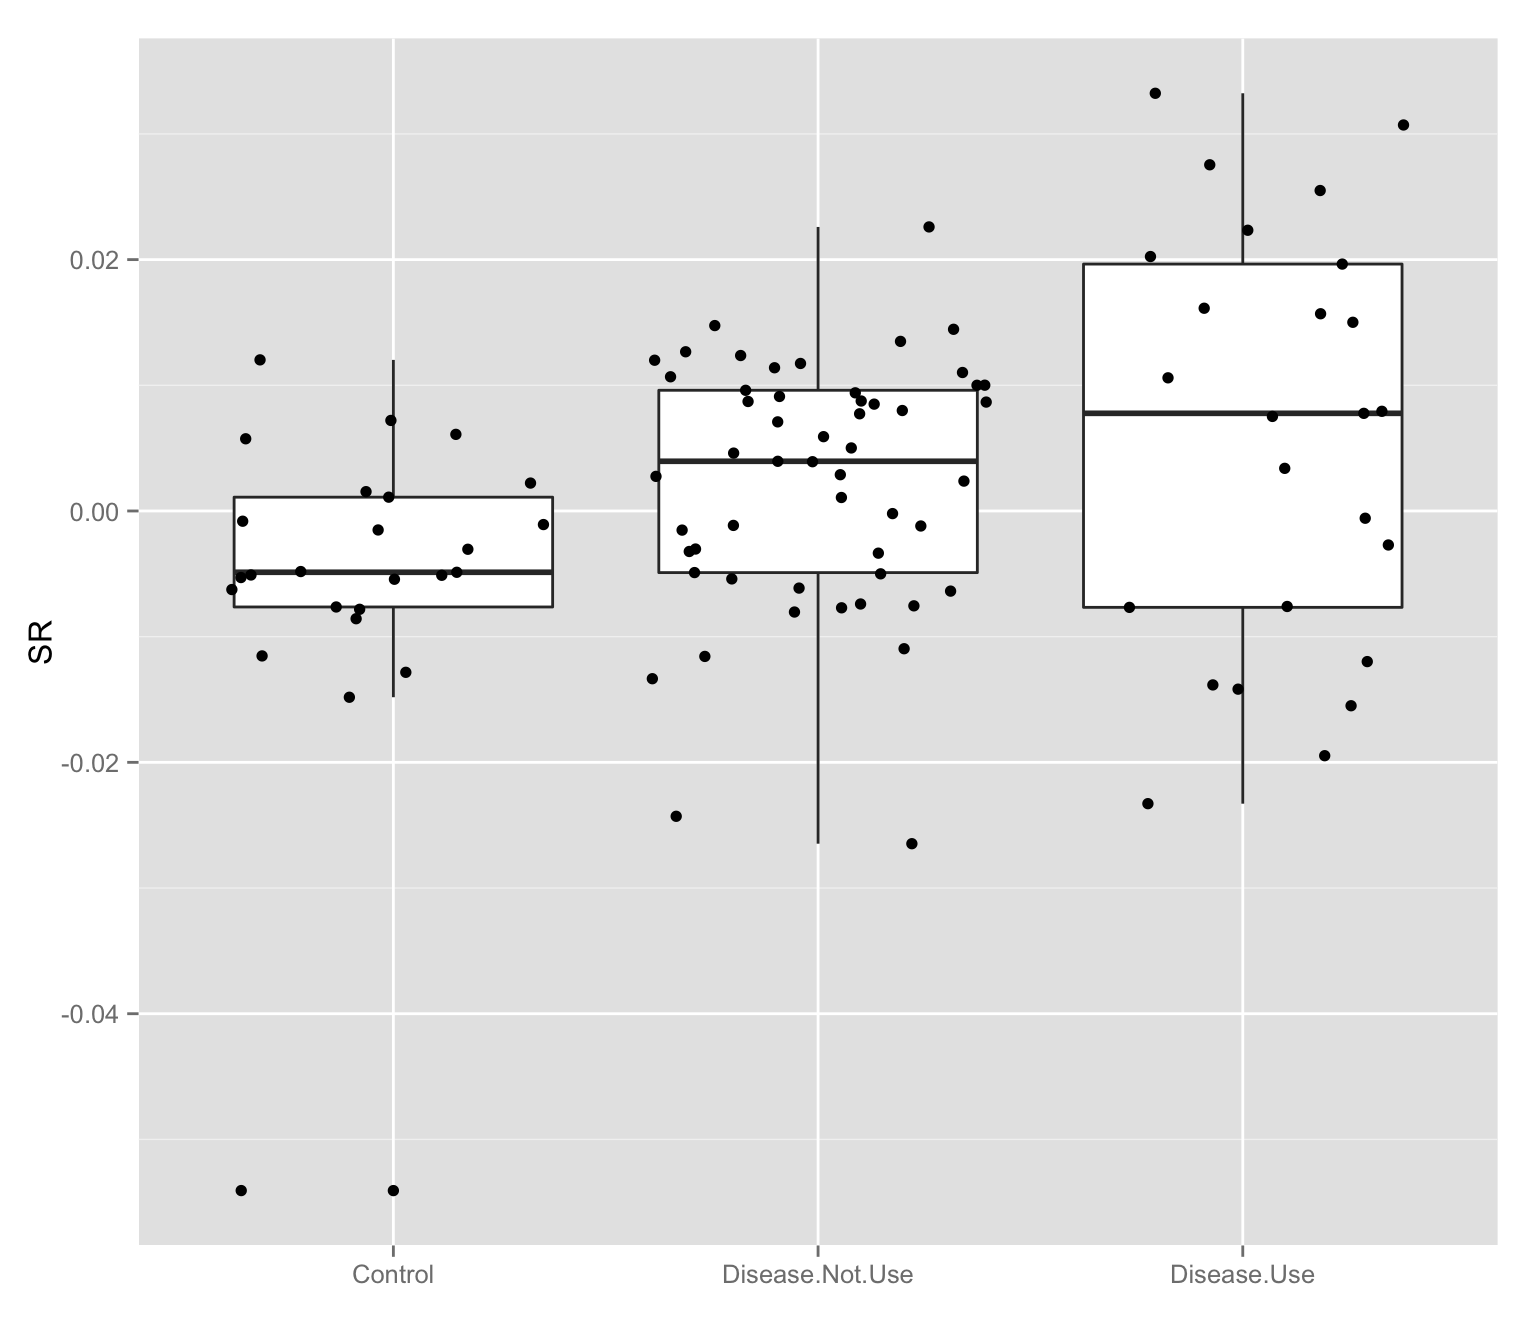
\includegraphics[scale=0.25,trim=0 0 0 0,clip]{Figure/F52_SR_control_disease_antibiotics.png}
}
\caption[Comparison of control and Crohn's disease samples stratified by antibiotic use with SR score]{Comparison of control and Crohn's disease samples stratified by antibiotic use with SR score.  K-mers (k=6) were extracted from the shotgun sequencing reads and the frequency of each k-mer was counted. Then multinomial inverse regression model was fitted to the k-mer count data and the sufficient reduction (SR) score was calculated. 
}
\label{F52_SR_control_disease_antibiotics}
\end{figure*}

In summary, microbiome is still a relative new and challenging research area. More advanced statistical models and efficient computational tools are still needed for metagenomic data analysis. I hope that this dissertation will provide new insight to other researchers in the field. 


\end{mainf}

% Use environment appendix1 if there is only 1 appendix (no numbering needed)
%\begin{appendix1}
%\chpt{Notation}
%\end{appendix1}


\begin{bibliof}
\printbibliography[title={BIBLIOGRAPHY}]
\end{bibliof}

\end{document}
